% BACHELORARBEIT MAIN
% Autorin.................................Neele Elbersgerd
\author{Neele \textsc{Elbersgerd}} 		% print with \authorname
% Erstellungsdatum........................10.08.2020


%--------IMPORT PRÄAMBEL
		% BACHELORARBEIT PRÄAMBEL
% Autor..................................Neele Elbersgerd
% Erstellungsdatum.......................10.08.2020

\documentclass[
fontsize=10pt, 
paper=a4, 
oneside,
%fleqn,  									% abgesetzte Formeln werden linksbündig ausgerichtet
%parskip=half+, 							% halber Zeilenabstand nach Absatz, +: min. ein Drittel der letzten Zeile eines Absatzes leer>> laut APA nicht nötig, daher raus
%headsepline = true,						%Linie unter Kopfzeile
headheight=30pt,
footheight=17pt,
abstract = true, 							% Überschrift im Abstract
%pointednumbers, 							% Punkt nach Gliederungszahl
toc=listof, toc=bibnumbered, 				% was soll in table of contents
listof=nochaptergap,
%toc=chapterentrywithdots,					% im toc auch Punkte zwischen Chapter und Seitenzahl
headings=optiontohead,						% optionale Befehle für Kolumnentitel
%noapacite,
numbers= noendperiod,
BCOR=8mm									% Bindekorrektur links --> wie viel?
]{scrreprt}
\AfterTOCHead{\linespread{1.25}\selectfont}	% Verzeichnisse mit kleinerem Zeilenabstand

% Allgemeines
		\usepackage[automark]{scrlayer-scrpage} 	% Kopf- und Fußzeilen
		\usepackage{amsmath,marvosym, amssymb} 		% Mathesachen
		\usepackage[TS1, T1]{fontenc} 				% Ligaturen, richtige Umlaute im PDF
		\usepackage[utf8]{inputenc}					% UTF8-Kodierung für Umlaute usw
		\usepackage[ngerman]{babel} 				% Silbentrennung
		\usepackage{mathtools} 						% mathematische Symbole
		\usepackage{upgreek}						% aufrechte griechische Buchstaben
		\usepackage[right]{eurosym}					% Eurosymbol
		\usepackage{siunitx}						% Einheiten
	%wie soll LaTeX bestimmte Wörter trennen?
		\hyphenation{Stab-elek-tro-de}
		\hyphenation{Haut-leit-wert-re-ak-tion}

% Absätze, Abstände, Seitenformat
		\usepackage[a4paper, left = 26mm, right = 26mm, top = 26mm, bottom = 26mm, 
		%showframe									% zeigt Satzspiegelränder
		]{geometry}    								% Textbreite
		%\setlength{\headsep}{0.7cm}				% Abstand zwischen Kopfzeile & Rumpf
		%\setlength{\footskip}{0.7cm}				% Abstand zwischen Fußzeile & Rumpf
		\usepackage{setspace} 						% 1.5 Zeilenabstand wie es üblicherweise 
			\setstretch{1.4}							% verstanden wird
		%\usepackage[onehalfspacing]{setspace}  	% eigentliche 1.5 Zeilenabstand

		\setlength{\parindent}{1.27cm}
		\usepackage{indentfirst} %um nach Überschrift 1. Indent nicht zu unterdrücken
		\renewcommand{\chapterheadstartvskip}{\vspace*{1\topskip}}	% Abstand von Kopfzeile zu Chapter-Überschrift
		\renewcommand{\chapterheadendvskip}{\vspace*{1\topskip}}	% Abstand von Chapter-Überschrift zu Text


% Überschriftenformatierung
		\renewcommand*{\chaptermarkformat}{\normalfont{ }}	% keine Nummerierung in Kopfzeile
		\renewcommand*{\raggedchapter}{\centering}			% Kapitelüberschriften mittig
		\RedeclareSectionCommand[beforeskip=-.25\baselineskip, afterskip=.25\baselineskip]{section}		% Abstand von Section Überschrift zu Text	
		\setkomafont{pagehead}{\normalfont{ }}		% Kopfzeilen vor Einleitung nicht kursiv
		
		%%%%%%SUSBSECTION 3. EBENE %%%%%%%%%
		%%%%%% VERSION Inline mit Einrückung %%%%%%%
			%\RedeclareSectionCommand[beforeskip=-.75\baselineskip, indent= 1.27cm, afterskip=-.5em]{subsection}		%afterskip: minus=In-Line Subsection Überschrift, Zahl = Abstand zum Folgetext,
		
		%%%%%% VERSION Outline ohne Einrückung %%%%%%%
			\RedeclareSectionCommand[beforeskip=-.25\baselineskip, afterskip=.25\baselineskip]{subsection}		%afterskip: minus=In-Line Subsection Überschrift, Zahl = Abstand zum Folgetext, 
		
		
% Schriftform & -größe
		\setkomafont{chapter}{\LARGE\rmfamily} 			% Überschrift der Ebene
		\setkomafont{section}{\Large\rmfamily}
		\setkomafont{subsection}{\large\rmfamily}
		\setkomafont{subsubsection}{\large\rmfamily}
		\setkomafont{chapterentry}{\large\rmfamily} 	% Überschrift in Inhaltsverzeichnis
		\setkomafont{descriptionlabel}{\bfseries\rmfamily} % für description-Umgebungen
		\setkomafont{captionlabel}{\small\bfseries}
		\setkomafont{caption}{\small}
		\usepackage{courier}							% für Zitation von Packages
		%\addtokomafont{disposition}{\Large} 			% Überschrift Abstract größer

% Tabellen
		\usepackage{multirow} 		% Tabellen-Zellen über mehrere Zeilen
		\usepackage{multicol} 		% mehrere Spalten auf eine Seite
		\usepackage{tabularx} 		% für Tabellen mit vorgegeben Größen
		\newcolumntype{C}{>{\centering\arraybackslash}X}	%centering Option in tabularx-float
		\usepackage{longtable} 		% Tabellen über mehrere Seiten
		\usepackage{array}			% zentrierte Elemente in Tabelle
		%\usepackage{rotating}     	% vertikaler Text in Tabellen
		\usepackage{booktabs}		% für Gestaltung horizontaler Linien
		\usepackage{chngcntr}		% counter für Tabellen-/Equation-/Figure-Nummerierung
			\counterwithout{table}{chapter}	% Tabellennummerierung unabhängig von Chapternr.
		\usepackage{caption}
		\DeclareCaptionLabelFormat{Nummerierung}{#1 #2}
		\captionsetup[table]{ 		% caption-package setup für Tab
			format=plain,  			% indention= generiert Einzug
			textfont={it, onehalfspacing, normalsize}, 	% Überschrift kursiv
			labelfont={normalfont,normalsize}, 			% Tabellennummerierung
			labelformat = Nummerierung,
			font=onehalfspacing,
			%width=.9\textwidth,	% feste Breite
			justification=justified,% Blocksatz
			singlelinecheck=false,	% damit Überschrift nicht zentriert, wenn einzeilig
			labelsep=newline,		% Abstand zw. Tabellennr. und Titel
			skip=0pt}				% Abstand zwischen Tabelle und Text davor
		\usepackage{threeparttable}
		% mglw. interessant: Use the siunitx package to align numbers with decimals
		\usepackage[table,xcdraw]{xcolor} 				% Farben

% Farben
		\definecolor{upblau}{HTML}{00305E} 				% uni potsdam blau
		\definecolor{upgrau}{HTML}{EBEBEB} 				% uni potsdam grau
		\definecolor{uporange}{HTML}{DF9945}			% humanwissenschaftsorange
		\definecolor{hrvbfborange}{HTML}{E46B0C}		% hrvbfb
		\definecolor{hrvbfbblau}{HTML}{00AFF4}  		% hrvbfb 
	

% PDF
		\usepackage[ngerman,pdfauthor={Neele Elbersgerd},  pdfauthor={Neele Elbersgerd}, pdftitle={Bachelorarbeit Psychologie}, pdfproducer	={LaTeX with hyperref},  
		breaklinks=true, 				% Zeilenumbruch bei links möglich
		bookmarks=true, 				% zeigt Lesezeichen in pdf an
		%colorlinks=true, linkcolor = up,	% wenn die Links farbig sein sollen
		linkbordercolor=upblau,				% für Farben der Kästen um Referenzen
		citebordercolor=upgrau,				% für Farben der Kästen um Zitationen
		urlbordercolor=uporange,			% für Farben der Kästen um URL-Links
		]{hyperref}
		\usepackage[final]{microtype} 	% mikrotypographische Optimierungen
		\usepackage{url} 				% ermöglicht Links (URLs)
		\usepackage{pdflscape} 			% einzelne Seiten drehen können
		\usepackage{pdfpages}      		% einbinden von pdf-Dateien




% Abbildungen
		\usepackage{graphicx} 			% Bilder
		\graphicspath{{images/}} 		% Standardpfad für Bilder
		\DeclareGraphicsExtensions{.pdf,.png,.jpg}	% bevorzuge pdf-Dateien vor den anderen
		\usepackage{subcaption}  					% mehrere Abbildungen übereinander
		\usepackage[all]{hypcap} 		% Klick auf Referenz führt zu Bild (nicht Caption)
		\usepackage{tikz}				% Zeichnungen in LaTeX
			\usetikzlibrary{positioning}
		\counterwithout{figure}{chapter}	% Abbildungsnummerierung unabhängig von Chapternr.
		\captionsetup[figure]{			% Captions bei Bildern
			format=plain,
			indention=0pt,				% kein Einzug
			labelsep=period,			% Punkt nach "Abbildung"
			labelfont=it,				% "Abbildung" kursiv
			margin={0pt,0.1\textwidth}, 	%rechter Rand, sodass Caption nur 90% von Textbreite
			justification=justified,
			singlelinecheck=false,
			font=onehalfspacing
		}
		%\setcapwidth[l]{0.9\textwidth} % Breite der Caption nur 90% der Textbreite
		%\setcapindent*{0em} 			% kein Einrücken der Caption von Figures und Tabellen
		\setlength{\abovecaptionskip}{0.3cm} % Abstand der zwischen Bild- und Bildunterschrift


%  Verzeichnisse & Bibliographie
		\setcounter{tocdepth}{\sectiontocdepth} 		% Gliederungstiefe ToC bis inkl. Section
		\usepackage{bibgerm} 							% Umlaute in BibTeX
		\usepackage[autostyle, german=quotes]{csquotes}	% deutsche Anführungszeichen
			
		%Anhang
		\newcommand*{\appendixmore}{		% siehe KOMA Doku S.339
			\renewcommand*{\chapterformat}{
				\appendixname~\thechapter\autodot\enskip}
			\renewcommand*{\chaptermarkformat}{
				\appendixname~\thechapter\autodot\enskip}}


%funktionierender BibLatex mit APA:	
		\usepackage[style=apa, 
		%apabackref=true, 			% Seitenangaben der Zitation im Verzeichnis
		backend=biber, 				% Biber als Backend
		hyperref=true, 				% Links in pdf
		%maxcitenames=6, maxnames=6, minbibnames=6, maxbibnames=6, % nur für bib
		apamaxprtauth=6, 			% max. 6 Namen, danach Auslassungszeichen
		%sorting = debug, 
		natbib=true, 
		language=ngerman, 
		doi=true, url=true, 
		%eprint=false,
		%useprefix=true,			
		uniquename=init 
		]{biblatex}
		\DeclareLanguageMapping{ngerman}{ngerman-apa}		% deutsceh Sprache
		\DefineBibliographyStrings{ngerman}{				% et al. darstellen
			andothers={et\ al\adddot}}	
		\addbibresource{./literature.bib} 			% Speicherort der Literatur
				
		%\DefineBibliographyExtras{ngerman}{\DeclareQuotePunctuation{.,}}
				

% Abkürzungsverzeichnis
		\usepackage{acronym}

% Quellcode		% für Formatierung in Quelltexten, hier im Anhang
		\usepackage{listings}
		\definecolor{grau}{gray}{0.25}
		\lstset{
			extendedchars=true,
			basicstyle=\tiny\ttfamily,
			%basicstyle=\footnotesize\ttfamily,
			tabsize=2,
			keywordstyle=\textbf,
			commentstyle=\color{grau},
			stringstyle=\textit,
			numbers=left,
			numberstyle=\tiny,
			breakautoindent  = true,		% für schönen Zeilenumbruch
			breakindent      = 2em,
			breaklines       = true,
			postbreak        = ,
			prebreak         = \raisebox{-.8ex}[0ex][0ex]{\Righttorque},
		}
		\usepackage{scrhack} 				% Vermeidung einer Warnung, die durch das Paket listings zum Anzeigen von Quelltext auftritt

% Fußzeile
		%\deffootnote{1.5em}{1em}{\makebox[1.5em][l]{\thefootnotemark}}	% linksbündige Fußnoten

% Eigene Befehle
	\newcommand{\leadingzero}[1]{							% führende Nullen (Datum)
		\ifnum #1<10 0\the#1\else\the#1\fi} 
	\newcommand{\todayI}{									% Datumsformat
		\leadingzero{\day}.\leadingzero{\month}.\the\year}			
	\newcommand{\mat}[1]{\mathbf{#1}} 						% Matrizen-Format
	\newcommand*{\ditto}{"}									% ditto marks
	\setcounter{equation}{0}					% für Referenzen der Gleichungen ab (1)
		\counterwithout{equation}{chapter}
		\renewcommand{\theequation}{\arabic{equation}}
		\newcommand{\nr}{\addtocounter{equation}{1}\tag{\theequation}}
	

%\typearea{14} % typearea berechnet einen sinnvollen Satzspiegel (das heißt die Seitenränder usw.) siehe auch http://www.ctan.org/pkg/typearea. Diese Berechnung befindet sich am Schluss, damit die Einstellungen von oben berücksichtigt werden
%\setlength{\parindent}{0pt}					% kein Einrücken im Text

	
		
\begin{document}

	\pagenumbering{roman} 	% Seitenummerierung mit römischen Zahlen für Tabellen- & Abbildungsverzeichnis
	\pagestyle{empty} 		% keine Kopf- oder Fußzeilen auf den ersten Seiten
	
	%--------TITELSEITE
		\begin{titlepage}
	
	\vspace*{0.5cm} 
	\begin{center}
		%--------FAKULTÄT & LOGO
				
				\begin{minipage}[t]{11cm}
							\vspace*{0.1cm}
							Universität Potsdam \\
							Humanwissenschaftliche Fakultät\\
							Department Psychologie\\
							Lehrstuhl für Emotions- \& Biopsychologie
				\end{minipage}
				\begin{minipage}[t]{3cm} \vspace{-\ht\strutbox}
							\begin{center} 
\includegraphics[width=\textwidth]{logoup} \end{center}
				\end{minipage} 
				  
		%--------TITEL & MITTELTEIL
			\vspace*{1.75cm}
	
				\begin{center}
						\rule{\textwidth}{0.5pt}\\			%Linie 1
						\vspace*{0.5cm}
						\doublespacing 
						\large{\textbf{
									%Verschiedene Lernprozesse in der Physiologie: \\		%Prozesse des Lernens?
									Vergleich der Verläufe von Schreck- und Hautleitwertreaktionen\\ %Schreckreaktion?
									in der Akquisitionsphase einer Furchtkonditionierung
									}}
									%Bilden Schreck- und Hautleitwertreaktion unterschiedliche Lernprozesse ab? Vergleich der Reaktionsverläufe in einer Furchtakqusition
						\vspace*{0.5cm} 
						%\normalsize Thesis Subtitle \\
						\rule{\textwidth}{0.5pt}			%Linie 2
						        
						\normalsize	\vspace*{0.25cm} 
						
									Bachelorarbeit vorgelegt von \\
									\textbf{Neele Katharina Elbersgerd} \\
						 			 zur Erlangung des akademischen Grades\\
						 			\textbf{ Bachelor of Science} \\ 
						 			im Studiengang Psychologie
				
						
					\end{center}    

			\vfill

				\begin{minipage}[t]{14cm}
							\begin{minipage}[t]{4.5cm}
									%vorgelegt von: \\
									Betreuerin:
									
									1. Gutachterin: 
									
									2. Gutachterin:\vspace{0.5cm} 
									
									
									E-Mail:
									
									Matrikelnummer:
									
									Einreichungsdatum:
							\end{minipage}
							\begin{minipage}[t]{9cm} 
									%Neele Katharina Elbersgerd \\				%Name
									\textbf{Dr. Julia Wendt}
									
									\textbf{Dr. Julia Wendt}
									
									\textbf{Dipl.-Psych. Miriam Hufenbach}\vspace{0.5cm}
									
									xxxxxxxxx@uni-potsdam.de 			%Email
									
									xxxxxx 							%Matrikelnr.
									
									19.05.2021							%Datum
							\end{minipage} 
				\end{minipage}

			\vspace*{1cm}
	\end{center}

\end{titlepage}
		
		\pagestyle{scrheadings} 	% Einstellen der Kopf und Fußzeilen für den Rest der Seiten
			\clearpairofpagestyles	% entfernt die default Kopf- und Fußzeile
			\ohead*{\pagemark}		% Seitenzahl oben rechts, *: auf jeder Seite
			\ihead*{\rightmark} 	% Kopfzeile zentriert mit Kapitelüberschrift

	%--------VERZEICHNISSE
		\tableofcontents 			% erstelle hier das Inhaltsverzeichnis
		%	\addchap*{Verzeichnisse} \listoffigures \listoftables
		\listoffigures				% erstelle hier das Abbildungsverzeichnis			
		\begingroup					% lof & lot auf gleicher Seite
			\let\clearpage\relax
			\listoftables			% erstelle hier das Tabellenverzeichnis
		\endgroup

		\addchap{Abkürzungsverzeichnis}		% erstelle das Abkürzungsverzeichnis
			
 \begin{acronym}[ANOVA]%[Bash] %immer das längste Akronym hier reinschreiben, damit Abstand angepasst wird
 	\itemsep2pt
		 	
		 	\acro{ANOVA}{Analysis of variance (dt.: Varianzanalyse)}
		 	\acro{ANS}{Autonomes Nervensystem}
		 	\acro{AV}{Abhängige Variable}
		 	%\acro{BSI}{Brief Symptom Inventory}
		 	\acro{BMI}{Body-Mass-Index}
		 	\acro{CR}{Conditioned Reaction (dt.: Konditionierte Reaktion)}
		 	\acro{CS}{Conditioned Stimulus (dt.: Konditionierter Stimulus)}
		 	%\acro{DSM-5}{Diagnostic and Statistical Manual of Mental Disorders, 5. Aufl.}
		 	\acro{EDA}{Elektrodermale Aktivität}
		 	\acro{EEG}{Elektroenzephalogramm}
		 	\acro{EKG}{Elektrokardiogramm}
		 	\acro{EMG}{Elektromyogramm}
		 	\acro{fMRT}{funktionelle Magnetresonanztomographie}
		 	\acro{FPS}{Furchtpotentierte Schreckreaktion}
		 	\acro{ITI}{Intertrial-Intervall}
		 	\acro{LRT}{Likelihood-Ratio-Test}
		 	\acro{KI}{Konfidenzintervall}
		 	\acro{MEM}{Mehrebenenmodell}
		 	\acro{ML}{Maximum-Likelihood}
		 	\acro{REML}{Restricted Maximum-Likelihood}
		 	\acro{SAM}{Self-Assessment Manikin}
		 	\acro{SCR}{Skin Conductance Response (dt.: Hautleitwertreaktion)}
		 	\acro{STR}{Startle Response (dt.: Schreckreaktion)}
		 	%\acro{STAI}{State-Trait-Angstinventar}
		 	\acro{UR}{Unkonditionierte Reaktion}
		 	\acro{US}{Unkonditionierter Stimulus}
		 	%\acro{WKA}{Wachstumskurvenanalyse???}
		 	
		 \end{acronym}\label{Zusammenfassung}

		%Befehle \addchap und \addsec, die jeweils eine nicht nummerierte Überschrift erstellen, aber auch für deren korrekten Eintrag ins Inhaltsverzeichnis und in die Kopfzeile sorgen.
	
	%--------ABSTRACT
		\clearpage
		\addchap{\abstractname}
%%%%%%%%%%%%%%%%%%%%%%%%%%%%%%%%%%%%%%%%%%%%%
%%%%%%%%%%%%%%% ABSTRACT %%%%%%%%%%%%%%%%%%%%
%%%%%%%%%%%%%%%%%%%%%%%%%%%%%%%%%%%%%%%%%%%%%
%aktuell 249 Wörter

\noindent 
%motivation and problem statement
 	In der Furchtkonditionierungsforschung sind Schreck- und Hautleitwertreaktionen (SCR) zwei der verbreitetsten Indikatoren, um  humane Furchtlernprozesse zu untersuchen. Allerdings herrscht Uneinigkeit darüber, inwiefern sie distinkte Lernprozesse widerspiegeln. Die Zwei-Prozess-Theorie nimmt an, dass differentielle Schreckreaktionen eine automatische Ebene des Furchtlernens indizieren, während differentielle SCR Kontingenzwissen auf kognitiver Ebene reflektieren.
% approach
	Diese Arbeit untersucht explorativ, ob sich in einer Furchtakquisition Unterschiede in Verläufen und Diskrimination Konditionierter Stimuli (CS) zwischen SCR und Schreckreaktionen abzeichnen, wenn beide statistisch gleichbehandelt in einem multivariaten Modell ausgewertet werden. 
	%Dafür werden Teildaten eines Großprojekts untersucht. 
	Achtunddreißig Versuchspersonen durchlaufen ein differentielles %, partiell verstärkten 
	Furchtakquisitionstraining, in dessen Verlauf ihnen zwei geometrische Reize mehrfach präsentiert werden. Einem folgt mit \SI{50}{\percent} Wahrscheinlichkeit ein elektrotaktiler Reiz. Nach der Hälfte des Trainings werden Versuchspersonen über die Reizkontingenzen aufgeklärt.
	Auswertungen erfolgen durch eine multivariate Wachstumskurvenanalyse (als Mehrebenenmodell). Mit dieser können Veränderungen zweier Variablen über die Zeit hinweg und die Variabilität zwischen Versuchspersonen modelliert werden. 		
% results
	Wichtigste Ergebnisse zeigen einen Interaktionseffekt zwischen CS und Zeit für die SCR -- nicht aber für die Schreckreaktionen --, der substanziell zwischen Versuchspersonen variiert. Mittelwertvergleiche und Visualisierungen verdeutlichen, dass eine Differenzierung zwischen den CS wenn, dann erst nach der Instruktion, auftritt.	
% conclusion
	Die gefundenen Effekte lassen sich schlussfolgernd nicht auf Furchtlernprozesse, sondern auf einen Instruktionseffekt zurückführen. Inferenzen auf die theoretische Indikation mehrerer Lernebenen lassen sich nicht ziehen.		
% future directions
	Nichtsdestotrotz werden wesentliche Vorteile, aber auch Hürden beim Einsatz von multivariaten Mehrebenenmodellen erläutert. 
	Dieser statistische Ansatz eröffnet neue Möglichkeiten zur Untersuchung und Integration mehrerer Furchtindikatoren und birgt das Potential, einen Beitrag zur Entschlüsselung der Mechanismen potentiell distinkter Furchtlernprozesse zu leisten.
	
	
\vspace*{0.5cm}
\noindent \textit{Schlagwörter:} Furchtakquisition, Hautleitwertreaktion, Schreckreaktion, Furchtlernen, Mehrebenenmodelle, Multivariate Verfahren

%Background, Methods, Results, Conclusions 

%Background & objectives, Methods, Results, Limitations, Conclusions

%Fragestellung, Hypothese, Merkmale der Versuchspersonen (z. B. Anzahl, Alter, Geschlecht), Methode, zentrale Ergebnisse sowie Schlussfolgerungen für die Hypothese.

%Fragestellung, Methode, Ergebnisse, Schlussfolgerungen.


%Beispiel Manon: Transkutane Vagus-Nerv-Stimulation (t-VNS) ist ein neues, nichtinvasives Neurostimulationsverfahren um den zervikalen Vagus-Nerv zu stimulieren, welches, vermutlich über die Aktivierung des Locus-Coeruleus-Noradrenalin-Systems, kognitive und affektive Prozesse beeinflusst. Mittels einem einfachblinden, randomisierten Studiendesigns untersuchte die folgende Studie die Effekte von t-VNS auf die Leistung von 61 gesunden Probanden bei einer lexikalischen Entscheidungsaufgabe und einem darauffolgenden Rekognitionstest. Hierbei erhielten Probanden entweder diskontinuierliche t-VNS (aktive Stimulation) oder diskontinuierliche Sham-Stimulation (Kontroll-Stimulation), während ihnen Wörter und Pseudowörter, die sich in ihrer emotionalen Valenz und in ihrer Abstraktheit unterschieden, präsentiert wurden. Des Weiteren wurde der Speichel-Alpha-Amylase (sAA) Spiegel als Biomarker für noradrenerge Aktivität vor und nach der Stimulation erfasst. Die Ergebnisse ergaben keine Hinweise auf Veränderungen des sAA Spiegels nach t-VNS. Dennoch konnte ein Interaktionseffekt von t-VNS und Wortvalenz im Rekognitionstest gezeigt werden, welcher darauf hinweist, dass t-VNS unterschiedliche Einflüsse auf die Reaktionszeit auf positive und negative Wörter hatte. Zudem waren sich Probanden aus der aktiven Stimulationsbedingung sicherer in ihren Entscheidungen an welche Wörter sie sich erinnerten und an welche nicht. Es konnte kein Einfluss von t-VNS auf Wortabstraktheit gefunden werden. Schlussfolgernd ist es unklar, ob das angewendete Stimulationsprotokoll zu einer erfolgreichen Stimulation des Vagus-Nervs geführt hat. Diese Ergebnisse betonen die Notwendigkeit, verlässliche Indikatoren für noradrenerge Aktivierung und optimale Stimulationsprotokolle weiter zu erforschen, um die Relevanz von t-VNS für potentielle Forschung (z.B. zu Gedächtnis, Emotionen) und für klinische Anwendungen (z.B. als therapeutisches Mittel) zu klären. 


%%%%%%%%%%%%%%%LEITFADEN BA
%Vollständigkeit: Das Abstract soll alle erforderlichen Informationen enthalten: Fragestellung, Hypothese, Merkmale der Versuchspersonen (z. B. Anzahl, Alter, Geschlecht), Methode, zentrale Ergebnisse sowie Schlussfolgerungen für die Hypothese.\\
%Genauigkeit: Inhaltliche Schwerpunkte und Terminologie des Textes sollen im Abstract beibehalten werden. Das Abstract darf keine Informationen enthalten, die im Manuskripttext nicht genannt werden.\\ 
%Objektivität: Das Abstract soll den Inhalt des Texts ohne Wertung wiedergeben.\\
%Kürze: Das Abstract soll so kurz wie möglich sein (nicht mehr als 250 Wörter); Unwesentliches, Wiederholungen sowie redundante Redewendungen sollen vermieden werden. Die APA empfiehlt weiterhin für Abstracts den Gebrauch von Ziffern statt verbaler Zahlbezeichnungen (außer am Satzanfang) und die Verwendung gebräuchlicher Abkürzungen (z. B. vs. statt versus), sowie der Verbform des Aktivs anstelle des Passivs (ohne die Personalpronomen ich und wir). Nichtlateinische Schriftzeichen, Symbole und Formeln sollten, wenn möglich, vermieden werden (wegen der Speicherung in Datenbanken mit begrenztem Zeichensatz).\\ 
%Verständlichkeit: Das Abstract soll klar und verständlich formuliert sein. Verschachtelte Sätze sollen vermieden werden; die wesentlichen Begriffe sollen in den Formulierungen deutlich hervortreten. Das Abstract muss auch ohne Fachkenntnisse, die über eine durchschnittliche psychologische Vorbildung hinausgehen, verständlich sein. Nicht allgemeingebräuchliche Abkürzungen müssen bei der ersten Nennung erläutert werden. Testverfahren sollen (bei der ersten Nennung) in ausgeschriebener Form angegeben werden.\\
	
	%--------INHALT
		\clearpage
		\pagenumbering{arabic} 		% ab jetzt arabische Nummerierung
			\addchap{Einleitung}
				

	Eine wesentliche Schwierigkeit in der experimentellen Forschung besteht seit jeher darin, Prozesse und Zustände, die man nicht direkt beobachten kann, greifbar zu machen. Es bedarf eines Indikators: eines Hilfsmittels, welches einen Zustand oder eine Entwicklung anzeigen und damit beobachtbar machen kann.  %lateinisch indicare „anzeigen“
	Ein Forschungsparadigma, für das sich diese Schwierigkeit in hohem Maße relevant zeigt, ist die Furchtkonditionierung. Mit ihr lassen sich unter anderem Prozesse wie das Furchtlernen untersuchen, bei dem auf Basis von vorherigen Erfahrungen negative Ereignisse antizipiert und vorsorgliche Schutz- oder Abwehrreaktionen in die Wege geleitet werden können. 
	Ein Verständnis für diese Prozesse und des ihnen zugrundeliegenden Furchtsystems ist von hohem Interesse. Zum Beispiel können fehlende Regulationsmechanismen in diesem anpassungsfähigen System mit pathologischen Mustern zusammenhängen, wie sie unter anderem bei Angststörungen festgestellt werden. Ein vollständiges Durchdringen der Mechanismen rings um die Entstehung und Aufrechterhaltung solcher Muster kann Behandlungs- und Forschungsmethoden verbessern und validieren.
	Anwendungsgebiete wie diese machen die Furchtkonditionierung zu einem wichtigen, experimentellen Paradigma.
	%If contained, fear is adaptive as it facilitates defensive responding, allowing the escape from, or avoidance of, dangerous situations, but if fear becomes exaggerated or is not appropriately regulated, it can develop into an anxiety disorder (Quinn & Fanselow, 2006)
	
	Um den Erwerb -- oder die Akquise -- von Furcht nachvollziehen zu können, werden verschiedene Indikatoren verwendet, wobei zwei physiologische Maße besonders verbreitet sind: die Hautleitwertreaktion und die Schreckreaktion. Bei erfolgreichem Furchtlernen wird typischerweise beobachtet, dass diese Reaktionen auf einen Reiz, der in der Vergangenheit ein negatives Ereignis vorhergesagt hat, höher ausfallen als auf einen, der diese Vorhersage nicht bereitstellt. Genannt wird diese Form des Furchterwerbs auch differentielles Furchtlernen.  
	Die Schreckreaktion besteht übergreifend aus einer körperlichen Kaskade an defensiven Bewegungen in Folge eines Schreckreizes, wobei das Schließen der Augen (die sogenannte Lidschlusskomponente) beim Menschen am häufigsten untersucht wird. In der Stärke der Schreckreaktion spiegelt sich unter anderem, wie angenehm oder unangenehm ein Reiz empfunden wird.
	Die Hautleitwertreaktion daneben beschreibt eine erhöhte Leitfähigkeit der Haut durch Schwitzen. Sie gilt vor allem als Maß für Erregung und reagiert besonders bei wichtigen oder neuen Stimuli. In Furchtkonditionierungsstudien wird sie ebenfalls traditionell als Indikator für Lernprozesse eingesetzt. 

	Eine immer noch aktuelle Fragestellung der Furchtkonditionierungsforschung ist, ob das Furchtlernen auf einem oder mehreren abgrenzbaren Prozessen basiert und welche Rolle das Bewusstsein über gelernte Verbindungen zwischen Reizen dabei spielt.
	Die Schreck- und die Hautleitwertreaktion werden dabei häufig als Indikatoren zweier verschiedener theoretischer Lernebenen herangezogen. Während die differentielle Schreckreaktion hauptsächlich mit einem automatischen und unbewussten Prozess in Verbindung gebracht wird, gilt eine Differenz in der Hautleitwertreaktion als Indiz eines kognitiven und bewussten Prozesses. 
	Ob diese Unterscheidung gerechtfertigt ist und inwiefern die beiden Maße tatsächlich unterscheidbare Informationen über Furchtlernprozesse bereitstellen, bleibt dabei größtenteils ungeklärt. 
	Im Kontext dieser Kontroverse hat diese Arbeit zum Ziel, die Verläufe der beiden Indikatoren in einer Furchtakquisition mittels eines multivariaten Verfahrens zu untersuchen. Durch diesen Auswertungsansatz können Limitationen herkömmlicher univariater Verfahren zum Teil überwunden und ein umfangreicher Einblick in das Zusammenspiel beider Maße gewonnen werden. 	
	Auf Basis dieses explorativen Ansatzes kann möglicherweise zu der Literatur rund um die Unterscheidung zweier konzeptueller Lernprozesse auf Reaktionsebene beigetragen werden.
	Außerdem erweitert die Arbeit die kaum bestehende Literatur, die Hautleitwert- und Schreckreaktion als physiologische Indikatoren in direkter Form miteinander vergleicht. 

	

%%%%%%%%%%%%%%%%%%%%%%%%%%%%%%%%%%%%%%%%%%%%%
%%%%%%%%%%%%%%%KAPITELÜBERBLICK%%%%%%%%%%%%%%
%%%%%%%%%%%%%%%%%%%%%%%%%%%%%%%%%%%%%%%%%%%%%

	Zu Beginn dieser Arbeit in Kapitel \ref{theorie} werden wesentliche Konzepte definiert und relevante Forschungsergebnisse eingeordnet. 
	Zunächst wird das grundlegende Paradigma der Furchtkonditionierung und ein Ausschnitt aus traditionellen und zeitgenössischen Konditionierungstheorien und -paradigmen beschrieben. 
	%Ohne Anspruch auf Vollständigkeit zu erheben, wird ein Ausschnitt aus traditionellen und zeitgenössischen Konditionierungstheorien thematisiert, um das Paradigma historisch und auch konzeptuell einzuordnen.
	Der anschließende Überblick über Indikatoren des Furchtlernens dient als Grundlage für den angestrebten Vergleich der Schreck- und Hautleitwertreaktionen, deren Methodik und Anwendung im Kontext der Furchtkonditionierung resümiert und verglichen wird.   
	%Dies ist die Grundlage für den Vergleich auf lerntheoretischer Ebene. 
	Die Fragestellung, ob Furchtlernen auf einem oder mehreren distinkten Prozessen basiert, wird anhand der sogenannten Ein-Prozess- und Zwei-Prozess-Theorien erläutert und außerdem einige der kontroversen Forschungsergebnisse diesbezüglich angesprochen. Hier spielen die Hautleitwert- und die Schreckreaktion als mögliche Indikatoren verschiedener Ebenen eine entscheidende Rolle.
	Auf diesen theoretischen Aspekten bauen die Ziele und exploratorischen Fragestellungen dieser Arbeit in Kapitel \ref{fragestellung} auf. In Kapitel \ref{methoden} gehe ich ausführlich auf die Methodik der Datenerhebung und Organisation dieser Arbeit sowie die verwendeten statistischen Analysen ein. Außerdem werden an dieser Stelle die Entscheidungskriterien für den multivariaten Modellbildungsprozess dargelegt. 
	Es folgt die Aufstellung des statistischen Modells und der Ergebnisbericht in Kapitel \ref{ergebnisse} sowie abschließend die Integration und Diskussion der Ergebnisse in Kapitel \ref{diskussion}. 



%%%%%%%%%%%%%LEITFADEN BACHELORARBEIT
		%Wichtig ist, dass potenzielle Leserinnen und Leser nach den ersten Sätzen (spätestens nach dem ersten Absatz) wissen, um was es in der Arbeit gehen wird und wieso die untersuchte Forschungsfrage von wissenschaftlichem Interesse ist .
		%im weiteren Verlauf der Einleitung dargestellt, welche Strategie man zur Beantwortung der Forschungsfrage bzw . zur Lösung des Problems gewählt hat
		
		%Diese Arbeit beginnt mit einer kurzen Einleitung zur Problemstellung (1-2 Seiten), in der das Thema psychologisch bzw. gesellschaftspolitisch eingeordnet wird, zentrale Konstrukte eingeführt werden sowie die Relevanz der Fragestellung deutlich wird. Zudem wird ein Überblick zu den nachfolgenden Kapiteln gegeben.
		%Leitfragen: Wird das Thema so eingeführt, dass auch Fachleute, die mit dem Themenbereich nicht vertraut sind, Inhalte und Relevanz der Arbeit einordnen können?
				%\addcontentsline{toc}{chapter}{Einleitung} 
				
			\chapter{Theorie und Stand der Forschung} 		\label{theorie}
				%%%%%%%%%%%%%%%%%%%%%%%%%%%%%%%%%%%%%%%%%%%%%
%%%%%%%%%%%EINLEITUNG%%%%%%%%%%%%%%%%%%%%%%%%%%%%
%%%%%%%%%%%%%%%%%%%%%%%%%%%%%%%%%%%%%%%%%%%%%

	Wenn wir Furcht empfinden, dann zumeist als Reaktion auf einen potenziell gefährlichen Reiz in unserer direkten Umwelt. Unser Körper begibt sich in einen erregten, defensiven Zustand und erhöht die Verhaltensbereitschaft für Flucht- oder Abwehrreaktionen. Furcht ist damit eine sehr adaptive und evolutionär relevante Emotion, die den Organismus vor Gefahr bewahren und möglichst schnell eine schützende Reaktion initiieren soll. In der psychologischen Forschung wird die Emotion Furcht typischerweise durch eine hohe Erregung und eine negative Valenz charakterisiert \parencite{LANG1995}.
	Welche Reize in der Umwelt als bedrohlich wahrgenommen werden, ist von verschiedenen Faktoren abhängig. Mittlerweile ist aber klar, dass Lernprozesse eine substanzielle Rolle dabei spielen. Unsere vergangenen Erfahrungen lenken unsere Wahrnehmung, Verarbeitung und Reaktion heute. Dieses erfahrungsbasierte Lernen -- oder \textit{Konditionierung} -- ist eine der Grundlagen für die Plastizität des Furchtsystems: Reize, die zuvor mit furchterregenden Ereignissen in Verbindung gebracht wurden, sind später in der Lage, selbst Furcht hervorzurufen. 

	In der psychologischen Grundlagen- und Anwendungsforschung werden Experimente zur Furchtkonditionierung seit knapp einem Jahrhundert für viele Fragestellungen eingesetzt. Die  Erkenntnisse führten in verschiedenen Disziplinen der Humanwissenschaften zu einem Boom an Abwandlungen des Paradigmas und Weiterentwicklungen in multiplen Forschungszweigen \parencite{MERZ2020}. Konzeptuell lassen sich Furchtkonditionierungsstudien in experimentelle Phasen unterteilen, die verschiedene Teilprozesse wie Furchterwerb, Extinktion und Wiederauftreten von Furcht zu modellieren versuchen. Innerhalb der Forschung um die Entstehung und Aufrechterhaltung von Angst- und Belastungsstörungen haben Furchtkonditionierungsexperimente entscheidende Einblicke in die Lern- und Gedächtnisprozesse von Menschen liefern können \parencite[für eine Übersichtsarbeit siehe][]{MINEKA2008}. Ebenso relevant sind sie für die (Weiter-)Entwicklung von Therapieelementen bei diesen Störungsbildern. Gerade dieser translationale Wert von Furchtkonditionierungsstudien trägt wesentlich zu ihrer unbestrittenen Relevanz bei.

	Die Fülle an Anwendungsgebieten mündete in einer Vielzahl an methodischen und terminologischen Variationen. Um eine bessere Vergleichbarkeit zu gewährleisten und Konsistenz in der Forschung zu fördern, haben \textcite{LONSDORF2017fc} Empfehlungen zur Methodik und Terminologie in Furchtkonditionierungsstudien zusammengestellt. Es sei zu Beginn darauf hingewiesen, dass methodische und technische Termini dieser Arbeit -- soweit nicht anders definiert -- im Einklang mit der Handreichung von \textcite{LONSDORF2017fc} zu verstehen sind. 

%%%%%%%%%%%%%%%%%%%%%%%%%%%%%%%%%%%%%%%%%%%%%
%%%%%%%%%%%DIE FURCHTKONDITIONIERUNG%%%%%%%%%%%%%%%%%
%%%%%%%%%%%%%%%%%%%%%%%%%%%%%%%%%%%%%%%%%%%%%

\section{Das Paradigma der Furchtkonditionierung}	\label{fearcondi}

	\subsection{Grundlagen der Klassischen Konditionierung}	\label{classic}

		Die Furchtkonditionierung beruht grundlegend auf dem Paradigma der Klassischen Konditionierung (auch Pavlovsche Konditionierung genannt). In seiner Pionierarbeit berichtete der russische Forscher \textcite{PAVLOV1927} von einer Konditionierung an einem Hund, an dessen Beispiel das Grundprinzip nachfolgend erläutert wird. 
		Die Klassische Konditionierung nutzt eine bereits bestehende Verbindung zwischen einem sogenannten Unkonditionierten Stimulus (US; hier Futter) und einer Unkonditionierten Reaktion (UR; hier erhöhter Speichelfluss beim Hund). Ein zunächst neutraler Stimulus -- bei Pavlov ein Glockenton -- löst wiederum eine neutrale Reaktion aus. In einem sogenannten \textit{Akquisitionstraining} wird der Glockenton wiederholt mit dem Futter (US) gemeinsam präsentiert, worauf der Hund mit erhöhtem Speichelfluss (UR) reagiert. Die Präsentation einiger dieser Paarungen führt dazu, dass der Glockenton zu einem \textit{Konditionierten Stimulus} (engl.: conditioned stimulus; CS) wird. Nach erfolgreichem Lernen ist die alleinige Präsentation des CS ausreichend, um den Speichelfluss auszulösen, der nun als \textit{Konditionierte Reaktion} (engl.: conditioned response; CR) bezeichnet wird. Diese CR ist in ihrer Modalität der UR meist ähnlich -- sprich, sie beschreiben das gleiche Verhalten -- allerdings ist die CR oft weniger intensiv.
		
		Die Furchtkonditionierung ist eine Variante dieses klassischen Paradigmas. Hier wird ein meist neutraler CS mit einem negativ valenten US (z.\,B. einem elektrotaktilen Stimulus) gepaart. Diese aversiven US lösen beim Individuum eine meist automatische (Furcht-)Reaktion wie den Schreckreflex aus. Diese Arbeit betrachtet die Akquisitionsphase einer Furchtkonditionierungsstudie. Hier wird mittels eines Akquisitionstrainings (der wiederholten gemeinsamen Präsentation von CS und US) eine konditionierte Reaktion manifestiert. Konzeptuell induziert dieses Training den Prozess des \textit{Furchtlernens}. 


	\subsection{Kognitive Erweiterungen}	\label{cognitive}

		Der Konditionierungsprozess wurde traditionell als simple und automatische Assoziationsbildung angesehen, die reflexiv und unfreiwillig erworben und abgerufen wird. Erst in den 70er Jahren wurde mit der \textit{kognitiven Wende} in der psychologischen Forschung den kognitiven Prozessen ein größerer Stellenwert eingeräumt. 
		Zum Beispiel zeigte \textcite{RESCORLA1968} in seiner Arbeit, dass die Kontingenz zwischen CS und US eine ausschlaggebende Rolle für den Erwerb einer CR spielt. Zudem lieferte er einen ersten Beleg dafür, dass die CS-US-Assoziation am besten gelernt wird, wenn der CS kurz vor dem US präsentiert wird. Diese Form der zeitlichen Kontiguität wird in der Furchtkonditionierungsforschung als \textit{Verzögerungskonditionierung} bezeichnet.
		Kognitive Ansätze dieser Art von Rescorla und anderen führten zu der weithin vertretenen Annahme, dass sich nach erfolgreichem Furchtlernen im Individuum die Erwartung an den US bildet, sobald ein CS dargeboten wurde. Diese US-Erwartung rückt die CR in die Position einer provisorischen Schutzreaktion auf Basis der gelernten Erfahrung, dass der US bald folgen wird \parencite{KIESEL2012}. Anders gesagt, kommt dem CS eine Prädiktorfunktion für den US zu. 
			
		Neben dem assoziativen Lernen im Sinne direkt erlebter Erfahrungen werden auch andere Pfade für das Furchtlernen in Betracht gezogen. \textcite {RACHMAN1977} postulierte neben der Konditionierung auch den Furchterwerb über Beobachtung und über Instruktionen. Beim beobachtenden Lernen observiert die Versuchsperson zum Beispiel die Furchtreaktion eines anderen Individuums auf einen Reiz, während sie beim instruktionalen Furchtlernen über die kausale Beziehung zwischen CS und US informiert wird. 
		Auch wenn dieser theoretische Ansatz nicht Gegenstand dieser Arbeit ist, gehe ich auf das instruktionale Furchtlernen kurz ein, da das verwendete Studiendesgin Instruktionselemente enthält (Abschnitt \ref{acq}).
		
		Instruktionen können die Versuchssubjekte teilweise oder vollständig über die vorhandenen CS-US-Kontingenzen aufklären. Während bei uninstruierten Designs erfahrungsbasiertes Furchtlernen über mehrere CS-US-Paarungen hinweg stattfinden kann, führt die explizite Aufklärung über die CS-US-Kontingenz sofort zu einer veränderten Furchtreaktion. Man spricht in diesem Fall von einem \textit{Furchtausdruck} statt von Furchtlernen \parencite{LONSDORF2017fc}. Diese erzwungene Bewusstwerdung kann einen erheblichen Einfluss auf den Lernprozess haben. Zum Beispiel zeigten \textcite{WEIDEMANN2016}, dass verbale Instruktionen über das Vorhandensein einer Beziehung zwischen CS und US das Auftreten von konditionierten Reaktionen (gemessen über die Lidschlusskomponente der Schreckreaktion) im Vergleich u.\,a. zu einer uninstruierten Gruppe erhöhen. Eine kürzlich erschienene Übersichtsarbeit von \textcite{MERTENS2018a} beleuchtet den moderierenden Effekt verbaler Instruktion auf die verschiedenen Phasen der Furchtkonditionierung tiefergehend (zur instruierten Extinktion sei auch die Übersichtsarbeit von \nptextcite{LUCK2016}, empfohlen). 
	
	
	
	\subsection{Das Differentielle Paradigma}	\label{differential}
	
		In der Furchtkonditionierungsforschung ist das sogenannte \textit{differentielle} Design eine relevante Erweiterung. Hierbei gibt es einen CS+, der immer oder manchmal mit einem US gepaart wird, und einen CS--, der niemals gemeinsam mit einem US auftritt. Typischerweise löst der CS+ eine stärkere CR aus und wird negativer bewertet als der CS--. Die Quantifizierung der Reaktionen kann zum Beispiel als differentielle CR erfolgen, sprich als Differenz der Reaktionen auf CS+ und CS--. In den überwiegenden Fällen sind CS+ und CS-- Reize ähnlicher oder gleicher Modalität (z.\,B. zwei unterschiedliche visuelle Stimuli). Die paradigmatische Ergänzung bietet mehrere Vorteile. Sie gewährleistet hinsichtlich des Erwerbs der CS-US-Kontingenz, dass der prädiktive Wert eines bestimmten Reizes gelernt und nicht das Vorhandensein eines Reizes an sich als Prädiktor missverstanden wird. Außerdem erlaubt das differentielle Konditionieren eine Kontrolle von möglichen Sensibilisierungseffekten. Das heißt, dass Effekte aufgrund der Modalität der CS vergleichbar zwischen CS+ und CS-- sind. 

	
%%%%%%%%%%%%%%%%%%%%%%%%%%%%%%%%%%%%%%%%%%%%%
%%%%%%%%%%%INDIKATOREN DES FURCHTLERNENS%%%%%%%%%%%%%%
%%%%%%%%%%%%%%%%%%%%%%%%%%%%%%%%%%%%%%%%%%%%%
	
\section{Indikatoren des Furchtlernens}	\label{index}
	
	Emotionen und Lernen haben als psychologische Konzepte eine wesentliche Sache gemeinsam: Auch
	wenn man eine Vorstellung von ihnen hat und sie relativ gut erkennt, so ist es gar nicht so leicht, sie richtig zu messen. Um das zu tun, müssen sie operationalisiert werden. 
	%Es fällt zum Teil leicht, sie zu erkennen, aber sie müssen operationalisiert werden, um quantifizierbar zu sein. 
	Beide Konstrukte sind komplexe Phänomene, die mit vielfältige Reaktionen auf verschiedenen Reaktionsdimensionen auslösen können.
	Diese können erfasst werden und ermöglichen es, Rückschlüsse auf eine bestimmte Emotion oder einen erfolgten Lernprozess zu ziehen.
	Furcht ist eine Emotion, die mit einer Aktivierung des Defensivnetzwerks einhergeht. Wenn Menschen Furcht empfinden, gibt es -- abhängig von der Proximität des furchtauslösenden Reizes -- eine Reihe an körperlichen Systemen, die in Gang gesetzt werden \parencite[zum menschlichen Defensivsystem siehe][]{HAMM2005, HAMM2006, OEHMANN2001}. Außerdem sind Menschen in der Lage, mitzuteilen, wie sich Furcht anfühlt. Ganz ähnlich ist das beim Lernen. In \textcite{KIESEL2012} wird Lernen definiert als "`Prozess, der als Ergebnis von Erfahrungen relativ langfristige Änderungen im Verhaltenspotential erzeugt"' (S. $11$). Allerdings reicht eine Änderung im Verhaltens\textit{potential} nicht, um Lernen experimentell nachweisen zu können. Es muss eine tatsächliche Änderung im Verhalten stattfinden, damit Rückschlüsse auf einen zugrundeliegenden Lernprozess gezogen werden können.
	
	Um nun Furchtlernen im Labor zu erfassen, kommen grundlegend drei Reaktionssysteme in Frage, die von \textcite{BRADLEY2000} in der Humanforschung unterschieden werden. Das sind (a) Handlung oder die Ausführung behavioraler Sequenzen (z.\,B. Flucht), (b) emotionale Sprache und (c) physiologische Reaktionen (z.\,B. steigende Herzrate). Die Veränderungen in Verhalten, physiologischen Reaktionen oder verbalen Berichten im Verlauf der Zeit sind damit klassische abhängige Variablen in Furchtkonditionierungsexperimenten.
	Bezogen auf die Furchtkonditionierung werden behaviorale Maße eher selten verwendet, am ehesten in Reaktionszeitexperimenten oder mittels Beobachtung von Vermeidungsverhalten. Verbale Maße sind häufiger: Sie können erfassen, inwieweit Subjekte explizites Wissen über CS-US-Kontingenzen erwerben ("`Der Reiz A sagt den Reiz B vorher"') oder wie die Bewertung von Affekt und Erregung sich im Laufe eines Experimentes ändert. 
	Physiologische Maße haben aufgrund ihrer Vergleichbarkeit mit Ergebnissen aus Tierstudien eine besonders wichtige Stellung in der Konditionierungsforschung. Unter den am häufigsten verwendeten Korrelaten sind peripherphysiologische Indikatoren wie die Herzrate, die Hautleitfähigkeit und die Schreckreaktion sowie neurobiologische Maße wie BOLD-Kontraste im fMRT oder Ereigniskorrelierte Potenziale im EEG. Die physiologischen Maße, vor allem diejenigen, die die Aktivität des autonomen Nervensystems (ANS) erfassen, gehen mit Vor- und Nachteilen einher. Ihr größtes Potential liegt darin, dass sie parallel zum Lernprozess erhoben werden können. Damit liefern sie einzigartige Informationen über körperliche Zustände, die zeitlich kontingent zum tatsächlichen Lernen geschehen. Allerdings sind sie -- anders als beispielsweise Ratings -- nicht oder zumindest nicht gleichermaßen furchtselektiv, was Inferenzen auf einzelne psychologische Prozesse erschwert (Abschnitte \ref{scrinference} und \ref{startleinference}).
	Zwei der am häufigsten verwendeten physiologischen CR sind die Lidschlusskomponente der Schreckreaktion und die Hautleitwertreaktion. Die folgenden Abschnitte erklären, wie sie erfasst werden, welche Körperprozesse sie abbilden und warum ihnen eine besondere Bedeutung zukommt.
	

%%%%%%%%%%%%%%%%%%%%%%%%%%%%%%%%%%%%%%%%%%%%%
%%%%%%%%%%%%%%%HAUTLEITWERTREAKTION%%%%%%%%%%%%%%%%
%%%%%%%%%%%%%%%%%%%%%%%%%%%%%%%%%%%%%%%%%%%%%

\section{Die Hautleitwertreaktion}		\label{scr}

	\subsection{Aspekte der Methodik}	\label{scrmethods}

		Die Hautleitwertreaktion (engl.: skin conductance response; SCR) ist ein Maß der Elektrodermalen Aktivität (EDA) und quantifiziert eine kurzfristige Änderung in der Leitfähigkeit der Haut in Reaktion auf einen Stimulus oder ein Ereignis. Sie ist ein weit verbreitetes und etabliertes Maß der Psychophysiologie. 
		Die Leitfähigkeit der Haut wird über Schweißdrüsen vermittelt und kann dort leicht und non-invasiv erfasst werden. Ekkrine Schweißdrüsen befinden sich fast überall am Körper, wobei ihre Dichte in der Handinnenfläche und an den Fingern mit am größten ist. Ableitungen der EDA werden präferiert dort vorgenommen \parencite{BOUCSEIN2012, DAWSON2007b}. In methodischer Hinsicht liegen die Vorteile der EDA darin, dass sie risikofrei, günstig und einfach zu erheben ist im Vergleich zu aufwendigeren physiologischen Methoden wie zum Beispiel dem EEG. Allerdings sind Hautleitwertreaktionen mit ihren $1$ bis \SI{4}{\second} Latenzzeit ein relativ langsames Maß \parencite{BOUCSEIN2012, DAWSON2007b}. Abgesehen von der Reaktionszeit unterscheidet sich die SCR von der Schreckreaktion auch dahingehend, dass kein zusätzlicher Auslösereiz benötigt wird, um sie zu erfassen (siehe Abschnitt \ref{startle} zur Schreckreaktion). 
		Im differentiellen Furchtkonditionierungsparadigma wird die SCR als Differenzmaß analysiert. Hier zeigte sich in zahlreichen Studien, dass durch erfolgreiches Lernen die Präsentation eines CS+ typischerweise eine höhere phasische Reaktion des Hautleitwerts hervorruft als die Präsentation eines CS-- \parencite{DAWSON1973, SEVENSTER2014}.
		Aufgrund der Latenzzeit der SCR muss bei dem Design von Furchtkonditionierungsstudien darauf geachtet werden, dass die Intertrial-Intervalle (ITI) zwischen zwei präsentierten Stimuli lang genug sind, damit die Hautleitwertreaktion auftreten und wieder abklingen kann \parencite{LONSDORF2017fc}.
		
		
	\subsection{Verwendung als Indikator}		\label{scrinference}
		%alternativ: „mögliche Inferenzen“
		
		Elektrodermale Maße werden in psychologischen Experimenten zur Erfassung vieler latenter Variablen und Prozesse herangezogen. Hautleitwertreaktionen sind als reliable Komponente der Orientierungsreaktion in Gegenwart von neuen, unerwarteten und signifikanten Stimuli \parencite{SIDDLE1991} weit verbreitet. Typischerweise wird beobachtet, dass die SCR bei wiederholter Präsentation in ihrer Amplitudenhöhe abnimmt. Dieser Habituationsverlauf geschieht zum Teil langsamer, je signifikanter (wichtiger) der Stimulus für das Individuum ist \parencite{BOUCSEIN2012}. Ein Beispiel für diese Signifikanz ist etwa die Relevanz des CS+ als Prädiktor für den US in einer Konditionierungsstudie. Zudem spielen auch Aufmerksamkeitseffekte und autonome Erregung eine nicht zu vernachlässigende Rolle in der Modulation von Hautleitwertreaktionen \parencite[für eine Ausführung siehe][]{DAWSON2007b}.
		
		Die Veränderung der EDA tritt weder in Isolation auf noch ist sie spezifisch für eine bestimmte Art von Reiz oder Kontext. Das bedeutet, dass die SCR oft nur eine Komponente in einer komplexen Reaktionskette des ANS abbildet. Diese kann wiederum durch verschiedene Einflüsse ausgelöst und moduliert werden, von Kontextbedingungen über Stimuluseigenschaften bis hin zum motivationalen und emotionalen Zustand, in dem sich die Versuchsperson befindet. Es ist typisch, dass Reaktionen, die die EDA beeinflussen, auch in andere Maße des ANS wie die Herzrate intervenieren. Tatsächlich müssen aber nicht alle diese Maße miteinander hoch korrelieren. Das liegt daran, dass Individuen immer wieder ein ihnen eigenes, relatives Reaktionsmuster des ANS produzieren und sich diese Muster aber interindividuell unterscheiden. Ein Phänomen, das als \textit{Individual Response Stereotypy} bekannt ist \parencite{ENGEL1960} und einen Grund dafür darstellt, dass für die Aktivierung des autonomen Nervensystems in der Forschung mehrere Indikatoren herangezogen werden. 
		
		Für sympathische Aktivität gilt die EDA hingegen als sehr spezifisches Maß. Ekkrine Schweißdrüsen und damit die EDA werden -- anders als andere Maße des ANS wie die Herzrate -- fast ausschließlich durch den Sympathikus kontrolliert \parencite{DAWSON2007b}. Die EDA kann dadurch mit der sympathischen Aktivierung infolge einer Defensivreaktion in Verbindung gebracht werden \parencite{MERZ2020}. Besonders responsiv zeigt sich die EDA in Situationen mit diskreten furchtauslösenden Stimuli, in denen eine Vermeidung nicht möglich ist \parencite{DAWSON2007b}. 
		Verwendet man die EDA nun als Indikator für Furchtlernen, bleibt jedoch das Problem der geringen Spezifität bestehen. Zwar konnten Studien zeigen, dass die SCR linear mit steigender induzierter Erregung der Stimuli ansteigt \parencite{LANG1990}, allerdings spielt sich dieser Effekt unabhängig von der Valenz der Stimuli ab. Im Kontext einer Konditionierung bedeutet das, dass ein CS gepaart mit einem aversiven US (Furchtkonditionierung) dasselbe Reaktionsmuster der EDA auslöst wie ein CS, der mit einem nicht-aversiven US gepaart wird \parencite{HAMM1996}.
		
		Ihre fehlende Spezifität wird der EDA häufig als Nachteil ausgelegt, denn durch ihre multikausale Bedingtheit ist sie kaum spezifisch interpretierbar. Trotz alledem ist ihre Bedeutung nicht von der Hand zu weisen. In den meisten experimentellen Designs hat das Ausmaß der Kontrolle einen entscheidenden Einfluss darauf, wie überzeugend und konkret SCR interpretiert und Inferenzen auf bestimmte psychologische Prozesse gezogen werden können \parencite{DAWSON2007b}. 
		
		
%%%%%%%%%%%%%%%%%%%%%%%%%%%%%%%%%%%%%%%%%%%%%
%%%%%%%%%%%%%%%SCHRECKREAKTION%%%%%%%%%%%%%%%%%%%
%%%%%%%%%%%%%%%%%%%%%%%%%%%%%%%%%%%%%%%%%%%%%


\section{Die Lidschlusskomponente der Schreckreaktion}		\label{startle}
		
	\subsection{Aspekte der Methodik}				\label{startlemethods}
		
		Die Schreckreaktion (engl.: startle reflex) beschreibt eine Reihe von protektiven motorischen Reflexen, die in Reaktion auf einen abrupten sensorischen Stimulus (engl.: probe stimulus; im Folgenden: Schreckreiz) ausgelöst werden \parencite{LANDIS1939}. Dieses Reaktionsmuster ist speziesübergreifend feststellbar und seine neuronalen Schaltkreise wurden in Tierstudien bereits eingehend erforscht und zum Teil in der Humanforschung repliziert \parencite[für eine Übersichtsarbeit siehe][]{DAVIS2006}. In letzterer erweist sich die Lidschlusskomponente (engl.: startle eye blink; im Folgenden allgemein: Schreckreaktion) als erste und stabilste Komponente, um diesen Schutzreflex systematisch zu erfassen \parencite{LANG1990}. Die Lidschlusskomponente beschreibt das reflexartige Zusammenkneifen der Augen infolge eines meist akustischen Schreckreizes. Wird dieser im Labor präsentiert, kann die Muskelkontraktion des Musculus Orbicularis Oculi über ein Elektromyogramm (EMG) aufgezeichnet werden. Die Elektroden hierfür werden zumeist auf der Hautoberfläche unterhalb des Auges angebracht. Der Schreckreiz ist meist ein \SI{50}{\milli\second} kurzes, $90$ bis \SI{105}{\decibel} lautes, weißes Rauschen und nach seiner Vergabe erfolgt die Schreckreaktion meist innerhalb von \SI{150}{\milli\second} \parencite{BLUMENTHAL2005}.
		Dadurch, dass diese Reaktion automatisch ausgelöst wird und sich damit der willentlichen Kontrolle entzieht, ist sie resistent gegenüber Effekten kognitiver Verarbeitung und Antworttendenzen, wie sie z.\,B. in verbalen Berichten auftreten können \parencite{LIPP2006, GRILLON2003}. Das ist methodisch ein Vorteil, da andere physiologische Maße wie die Herzrate und die Hautleitfähigkeit durchaus – wenn auch in begrenztem Maß -- aktiv durch die Versuchspersonen beeinflusst werden können \parencite[z.\,B. mit Beeinflussung der Atmung;][]{LONSDORF2017fc}.
		
		Bei Verwendung in Furchtkonditionierungsstudien ist ein wesentlicher methodischer Vorteil der Schreckreaktion, dass sie circa um das $50$-fache schneller nach Reizdarbietung auftritt als die Hautleitwertreaktion. %(min. $20$\,ms versus min. $1$\,s)
		Außerdem weist sie eine kürzere Refraktärzeit auf. Durch diesen zeitlichen Vorteil kann die Schreckreaktion zu jeder Zeit während des Furchtakquisitionstrainings ausgelöst werden und wichtige zeitlich kontingente Einblicke liefern \parencite{LIPP2006}. Im Gegensatz zur SCR ist es außerdem möglich, Reaktionen innerhalb der ITI zu erheben und damit eine Basisreaktion unabhängig von der CS-Präsentation zu definieren. Die Erfassung der Schreckreaktion als Furchtmaß benötigt allerdings eine Habituationsphase, in der der Schreckreiz zwei bis zehn Mal präsentiert wird. Damit soll gewährleistet werden, dass die ersten starken Reaktionen auf den Schreckreiz den Verlauf der CR in Reaktion auf einen Stimulus weniger beeinflussen \parencite{BLUMENTHAL2005}. Eine Phase wie diese ist bei Erhebung der SCR nicht nötig. 
		
	\subsection{Verwendung als Indikator}				\label{startleinference}
		
		In den allermeisten Fällen, in denen die Schreckreaktion experimentell erhoben wird, geht es nicht primär um den motorischen Reflex als solchen, sondern um die psychologischen Prozesse, mit denen er in Verbindung gebracht wird. Die Relevanz der Schreckreaktion für die Furchtkonditionierungsforschung begründet sich durch ihre relative Spezifität zur Erfassung von Furcht. 
		\textcite{LANG1990} zeigten, dass die Schreckreaktion durch Affekt moduliert wird. Während angenehme Reize die Schreckreaktion hemmen, wird sie durch unangenehme Stimuli potenziert. Dieses Phänomen ist im Kontext der Furchtkonditionierung als Furchtpotenzierung der Schreckreaktion (FPS) bekannt: Ein bereits konditionierter Stimulus (CS+) löst eine stärkere Schreckreaktion aus als ein nicht-verstärkter CS-- \parencite{BROWN1951, HAMM1996, HAMM2005, BRADLEY2005}. Die FPS tritt unabhängig von der Neuheit der Reize auf. Zwar nimmt die Reaktion in absoluten Werten bei mehreren Trials mit der Zeit ab, der Effekt der emotionalen Modulation bleibt jedoch robust bestehen \parencite{BRADLEY2000}. Zudem zeigten \textcite{CUTHBERT1996}, dass Erregung die Schreckreaktion auf aversive Reize zusätzlich moduliert. Die Potenzierung der Schreckreaktion zeigt sich bei der Präsentation von hoch erregenden und negativ valenten Stimuli, allerdings nicht bei wenig erregenden und trotzdem negativ valenten Reizen \parencite{CUTHBERT1996}. Ein daraus resultierender Vorteil ist, dass die Schreckreaktion Furchtlernen verhältnismäßig spezifisch erfassen kann. Im Vergleich mit der Hautleitwertreaktion, die eher valenzunspezifische Erregung reflektiert, wird der Schreckreaktion die Rolle als spezifischerer Furchtindikator zugedacht \parencite{HAMM1996}. 
		
		Die neuroanatomische Basis wurde vielfach in tierexperimentellen Studien untersucht. Zahlreiche Studien, u.a. von Davis und Kolleg*innen, lieferten übereinstimmende Evidenz dafür, dass die Potenzierung der Schreckreaktion über die Amygdala vermittelt wird \parencite[für eine Übersichtsarbeit siehe][]{DAVIS2006}. Die Amygdala ist eine limbische Struktur im medialen Temporallappen und gilt als eine zentrale Schaltstelle des Defensivsystems \parencite{HAMM2006, DAVIS1992}. Mit ihren efferenten Projektionen initiiert und mediiert die Amygdala Furchtsymptome wie körperliche Erregung oder protektive motorische Reflexe, wozu auch die Schreckreaktion gehört. 
		Bei Läsionen des zentralen Kerns der Amygdala findet die Schreckreaktion auf einen Schreckreiz durchaus statt, allerdings wird sie bei Furchtreizen nicht mehr potenziert \parencite{HITCHCOCK1987, HITCHCOCK1986}. Das macht die Schreckreaktion zu einem validen Indikator für die Aktivierung des Defensivsystems.
		
		Ein methodischer und theoretischer Nachteil im Vergleich zur SCR ergibt sich durch die Notwendigkeit eines zusätzlichen Schreckreizes zum Auslösen der Schreckreaktion. Es ist bereits gezeigt worden, dass die physikalischen Eigenschaften des Schreckreizes die Schreckreaktion in Intensität und Onset modulieren \parencite{BLUMENTHAL2005}. Außerdem wird der Schreckreiz von Versuchspersonen ebenfalls häufig als aversiv wahrgenommen. Ein potentieller Einfluss auf den emotionalen Zustand der Person und demnach auch auf die Intensität des Schreckreflexes kann nicht ausgeschlossen werden \parencite{LIPP2006}. \textcite{SJOUWERMAN2016} konnten außerdem zeigen, dass die Inklusion von Schreckreizen in einer Furchtkonditionierungsstudie die Furchtakquisition verzögerte (gemessen anhand der SCR). Die Wahl der abhängigen Variable(n) hat demnach durchaus einen nicht zu unterschätzenden Einfluss auf den Lernprozess.
		
		
%%%%%%%%%%%%%%%%%%%%%%%%%%%%%%%%%%%%%%%%%%%%%
%%%%%%%%%%%%%%MEHRERE OUTCOMES%%%%%%%%%%%%%%%%%%%
%%%%%%%%%%%%%%%%%%%%%%%%%%%%%%%%%%%%%%%%%%%%%
			
\section{Verwendung mehrerer Indikatoren}			\label{outcome}

	Furchtlernen gilt als Konstrukt mit einem komplexen Aktivierungsnetzwerk. Die eingesetzten Indikatoren können nicht distinkt in die spezifische Erfassung von Kontingenzwissen, konditionierter Reaktion, Aufmerksamkeitsverarbeitung oder emotionalem Zustand eingeordnet werden \parencite{LIPP2006}. Es hat sich während der letzten Forschungsjahrzehnte etabliert, mehrere Indikatoren gleicher oder unterschiedlicher Reaktionsebenen zur Erfassung von Furchtlernen zu verwenden, um ein vollständigeres Bild der Prozesse zu erhalten. Nach \textcite{LIPP2006} ging diese wichtige Änderung mit der Realisierung einher, dass einzelne Maße unterschiedliche Spezifitäten aufweisen. Verbale Maße sind oft durch Antwort- und Erinnerungstendenzen verfälscht. Physiologische Maße reflektieren nicht nur Furcht, sondern werden ebenfalls durch Prozesse wie Aufmerksamkeit oder Kontexteffekte beeinflusst. Es wird auch in der Empirie deutlich, dass Indikatoren verschiedener Ebenen oft nur in geringem Maße kovariieren \parencite{BRADLEY2000, LIPP2006}. 
	Ein verwandtes Problem beim Verwenden mehrerer Maße ist, dass sich die Indikatoren auch in ihrer Sensitivität unterscheiden. Der direkte Vergleich von unterschiedlichen CR, vor allem über verschiedene Studien hinweg, gestaltet sich als schwieriges Unterfangen. 
	Zusammenfassend bedeutet das: Ein einzelnes Maß kann viele Komponenten abbilden, währenddessen sich die gewünschten Effekte in mehreren Maßen gleichzeitig widerspiegeln können.
	Die Integration mehrerer Indikatoren genauso wie das Wissen um ihre Interdependenzen sind entscheidende Bausteine der aktuellen und zukünftigen Furchtkonditionierungsforschung. 
	
	Die steigende Komplexität, die die Wahl der abhängigen Variablen mit sich bringt, ist auch zunehmend Gegenstand der Forschungsliteratur. Neben den bereits zitierten Empfehlungen und Richtlinien von \textcite{LONSDORF2017fc} haben auch \textcite{OJALA2020} erst kürzlich eine Übersichtsarbeit über verschiedene Arten konditionierter Reaktionen veröffentlicht. Darin beurteilten sie verschiedene CR unter anderem nach ihrer Qualität, Inferenzen auf gebildete CS-US-Assoziationen zu ermöglichen. Eine Studie von \textcite{LEUCHS2019} verglich die Indikatoren SCR und Schreckreaktion mit der an Aufmerksamkeit gewinnenden Pupillendilatation als CR einer Furchtkonditionierung. Die Akquisitionsdaten zeigen signifikante, aber eher geringe Korrelationen zwischen allen drei Maßen (trialweise gemittelt; für SCR und FPS $r=.16$, $p<.001$, \nptextcite{LEUCHS2019}). Sowohl die SCR als auch die FPS unterlagen einer starken Habituation, diskriminierten aber beide signifikant zwischen CS+ und CS-- \parencite{LEUCHS2019}.
	Relevant für den Einsatz mehrerer Reaktionsmaße ist auch, dass sich verschiedene CR durchaus gegenseitig beeinflussen \parencite{LONSDORF2017fc}. Das liegt nicht nur daran, dass Trials und ITI in Rücksicht auf die Onset- und Refraktärzeiten der Hautleitwertreaktion zeitlich koordiniert werden müssen, sondern auch an der Wechselwirkung von CR an sich. Dazu gehört zum Beispiel die bereits erwähnte Studie von \textcite{SJOUWERMAN2016}, bei der das Verwenden von akustischen Schreckreizen das Furchtlernen, gezeigt an der SCR, verzögert. Ein weiterer, wichtiger Aspekt ist die umstrittene Annahme, dass unterschiedliche Indikatoren verschiedene inhaltliche Prozesse des Furchtlernens abbilden. Im Folgenden wird dieser Disput in der Forschung näher erläutert.


%%%%%%%%%%%%%%%%%%%%%%%%%%%%%%%%%%%%%%%%%%%%%
%%%%%%%%%%%%%%LERNTHEORETISCH%%%%%%%%%%%%%%%%%%%%%
%%%%%%%%%%%%%%%%%%%%%%%%%%%%%%%%%%%%%%%%%%%%%
	
\section{Lerntheoretische Perspektiven}			\label{processes}

	\subsection{Ein oder zwei Systeme?}			\label{singledual}

		Ursprünglich wurde der Konditionierungsprozess als simple, beinahe mechanische Bildung von Assoziationen unabhängig von kognitiven Mechanismen verstanden \parencite{LOVIBOND2006}. Es ist mittlerweile größtenteils unbestritten, dass auch kognitive Mechanismen (wie die Abhängigkeit des Lernens von Kontingenz und Kontiguität, \nptextcite{RESCORLA1968}) bei der Erklärung von Furchtlernphänomenen eine nicht zu unterschätzende Rolle spielen. In diesem Zusammenhang werden häufig zwei aktive Systeme angenommen, sobald Menschen Reizkontingenzen beim klassischen Konditionieren ausgesetzt sind: zum einen das automatische, reflexive System und zum anderen das propositionale, kognitive System \parencite{LOVIBOND2006}. Diese Dualitätsannahme taucht in verschiedenen Ansätzen zu Lern- und Gedächtnisprozessen mit jeweils kleinen Abweichungen immer wieder auf. Begrifflich werden theoretische Differenzierungen zwischen dem expliziten und dem impliziten, dem bewussten und dem unbewussten oder dem kontrollierten und dem automatischen Lernen vorgenommen. Die Idee von zwei \textit{Ebenen des Lernens} beim menschlichen Assoziationslernen reflektiert sich in den verschiedenen dualen Lerntheorien. Doch auch wenn der lernbasierte Ansatz und die substanzielle Bedeutung von Kognitionen in Lernprozessen allgemein akzeptiert bleibt, ist das Vorhandensein dualer oder mehrerer Prozesse an sich ein umstrittenes Thema.

		In der Furchtkonditionierungsforschung beschäftigt sich der Diskurs damit, ob überhaupt distinkte Prozesse am Klassischen Konditionieren beteiligt sind. Ein Fokus liegt hier auf dem Konflikt um die Notwendigkeit des Bewusstseins für das Zeigen einer konditionierten Reaktion \parencite[für systematische Übersichtsarbeiten siehe][]{LOVIBOND2002, MERTENS2020}. Es wird unter anderem darüber disputiert, ob und zu welchem Grad die Konditionierung beim Menschen von einem bewussten Verständnis der gelernten Kontingenz abhängt und welche Operationalisierung für Bewusstsein hierfür herangezogen werden kann. Maßgeblich wird der Konflikt von zwei Polen bestimmt. Die \textit{Zwei-Prozess}-Theorie vertritt die Auffassung von zwei unabhängigen Prozessen des Lernens \parencite{HAMM1996, HAMM2005, OEHMANN2001, WEIKE2007}. Zum einen führt ein propositionaler, kognitiver Lernvorgang zu verbalisierbarem Kontingenzbewusstsein. Zum anderen wird auf einer nicht-propositionalen, impliziten Ebene eine autonome CR wie die Schreckreaktion produziert. 
		Die \textit{Ein-Prozess}-Theorie steht dem gegenüber. Vertreter*innen dieser Annahme kritisieren, dass in Studien zum Klassischen Konditionieren beim Menschen kein hinreichender Nachweis für die Notwendigkeit von Bewusstsein -- und damit für das Vorhandensein zweier Ebenen -- erbracht wurde. Der Ein-Prozess-Ansatz geht von nur einer Ebene aus, die einen propositionalen Lernprozess beschreibt \parencite{LOVIBOND2002, DEHOUWER2014, DEHOUWER2009, MITCHELL2009, MERTENS2020}. In seiner stärksten Form wird angenommen, dass Kontingenzbewusstsein eine Voraussetzung für das Auftreten einer CR ist. Personen müssen demnach in der Lage sein, explizit die Beziehung zwischen CS und US zu beschreiben, um konditionierte Reaktionen zu zeigen. In einer schwächeren Form der Ein-Prozess-Theorie sind sowohl Kontingenzbewusstsein als auch CR ebenbürtige Endpunkte des propositionalen Lernprozesses, die allerdings stark miteinander korrespondieren. 

		Die Forschungsergebnisse zu dem Disput sind bis heute ambig. Unter anderem kritisierten \textcite{LOVIBOND2002} die Operationalisierung und Erfassung von Kontingenzbewusstsein und bemängelten, dass kein hinreichender Nachweis für einen Dualismus oder ein Konditionieren ohne Bewusstsein erbracht worden sei. Außerdem erweise sich die unterschiedliche Methodik in der Durchführung von Konditionierungsstudien als Schwierigkeit für die Interpretation und Vergleichbarkeit unterschiedlicher Forschungsergebnisse. In ihrer aktuellen Metaanalyse verzeichneten \textcite{MERTENS2020}, dass $39$ von $41$ inkludierten Studien mindestens einem methodischen Problem unterlagen. Dazu gehören unter anderem die Erfassung von Kontingenzbewusstsein und Entscheidungsfreiheiten der Wissenschaftler*innen in Bezug auf Ausschlusskriterien und Kennwertbestimmung.
		
		Auch wenn grundlegend relevant für die aktuelle Forschung, so wird das Konstrukt \textit{Kontingenzbewusstsein} als solches und der Disput um seine Operationalisierung nicht näher in dieser Arbeit betrachtet.
		Interessierte Leser*innen seien zum Beispiel an die Arbeiten von \textcite{LOVIBOND2002}, \textcite{WIENS2002} oder \textcite{MERTENS2020} verwiesen. Im nächsten Abschnitt folgt ein Überblick über Forschungsergebnisse, bei denen Hautleitwert- und Schreckreaktionen als Indikatoren verschiedener Lernprozesse herangezogen wurden. 
		Dies dient als Grundlage für die Herleitung der Fragestellung und Analyse in dieser Arbeit.

	\subsection{Schreck- und Hautleitwertreaktion als Indikatoren unterschiedlicher Lernebenen}	\label{dissociation}
		
		Insbesondere im Rahmen der Zwei-Prozess-Theorie werden Schreck- und Hautleitwertreaktionen als Indikatoren verschiedener Lernebenen herangezogen \parencite{HAMM1996, SEVENSTER2014}. Es wird angenommen, dass die FPS das implizite und emotionale Furchtlernen reflektiert und unabhängiger von kognitivem Wissen über die Stimulusrelationen auftritt \parencite[z.\,B.][]{SEVENSTER2014, HAMM2005}. Dagegen wird die differentielle SCR grundlegend mit Kontingenzlernen und dem US-Erwartungslernen in Verbindung gebracht \parencite[z.\,B.][]{HAMM2005, WEIKE2007}. US-Erwartung beschreibt, wie groß die Erwartung der Versuchspersonen an einen US ist, nachdem ein bestimmter CS präsentiert wurde. Allerdings ist der Zusammenhang zwischen SCR und Kontingenzbewusstsein umstritten.
		Es herrscht konkurrierende Evidenz darüber, ob das Zeigen einer differentiellen SCR vom Kontingenzbewusstsein der Person abhängt \parencite{DAWSON1973, HAMM1996, PURKIS2001, WEIKE2007} oder nicht \parencite{KNIGHT2003, SCHULTZ2010}.
		
		Ein Beispiel für die Dissoziation zwischen SCR und Schreckreaktion in einem differentiellen Furchtkonditionierungsparadigma lieferten \textcite{SEVENSTER2014}. Sie reproduzierten eine Studie von \textcite{SCHULTZ2010}, bei der eine Gruppe auf ein einfaches und eine andere auf ein schwierig zu diskriminierendes Paar von CS+ und CS-- konditioniert wurde. \textcite{SCHULTZ2010} fanden eine differentielle US-Erwartung ursprünglich nur in der leichten Bedingung, während beide Gruppen eine differentielle SCR zeigten. Daraus schlussfolgerten sie, dass die differentielle SCR nicht durch Kontingenzbewusstsein beeinflusst wird \parencite{SCHULTZ2010}. In ihrer Replikationsstudie verwendeten \textcite{SEVENSTER2014} dasselbe Set an Stimuli und erfassten zusätzlich die Schreckreaktion als Indikator. Ihre Ergebnisse zeigten, dass die differentielle SCR nur bei den Versuchspersonen auftrat, die deklaratives Wissen über die CS-US-Kontingenz aufgebaut hatten (erfasst über Befragungen zur US-Erwartung während des Trainings). Eine differentielle Schreckreaktion zeigte sich unabhängig vom Kontingenzwissen. Diese Daten unterstützen die Zwei-Prozess-Theorie und lassen vermuten, dass die Hautleitwertreaktion im Gegensatz zur Schreckreaktion mit bewusstem Lernen über die Stimuluskontingenzen zusammenhängt. 
		Die Ergebnisse der Studie von \textcite{WEIKE2007} deuten zudem auf eine Abhängigkeit dieser potentiellen Dissoziation von der Methodik der CS-US-Paarungen hin. In einem Vergleich zwischen Spuren- und Verzögerungskonditionierung zeigte sich die differentielle SCR in beiden Gruppen nur bei Personen, die Kontingenzbewusstsein aufwiesen (erfasst über ein Interview nach dem Training). Die konditionierte FPS allerdings trat in der Gruppe mit Verzögerungskonditionierung unabhängig vom Bewusstsein auf, während sie bei der Gruppe mit Spurenkonditionierung nur bei Personen mit Kontingenzbewusstsein zu finden war. 
		Daraus lässt sich schließen, dass auch methodische und zeitliche Aspekte des Furchtakquisitionstrainings einen Einfluss darauf haben, inwiefern Schreck- und Hautleitwertreaktionen als Indikatoren zweier distinkter Lernprozesse herangezogen werden können. Limitiert wird die Interpretierbarkeit dieses Ergebnisses durch die Erfassung von Kontingenzbewusstsein nach dem Akquisitionstraining, wodurch Gedächtniseffekte nicht ausgeschlossen werden können \parencite{MERTENS2020}. 
		
		Auf der anderen Seite gibt es auch Befunde, die keine Nachweise für Furchtkonditionierung der Schreckreaktion in Abwesenheit von Kontingenzbewusstsein finden und demnach keine Inferenz auf distinkte Prozesse zulassen. In einer Furchtakquisitionsstudie mit Verzögerungskonditionierung von \textcite{PURKIS2001} zeigten sich differentielle Hautleitwertreaktionen nur für die Versuchspersonen, die Kontingenzbewusstsein aufwiesen. Das gleiche Muster zeichnete sich allerdings auch für die Schreckreaktionen ab, was nahelegt, dass die FPS abhängig vom Kontingenzbewusstsein der Versuchspersonen ist.
		Ähnliche Ergebnisse erbrachte die Studie von \textcite{GRILLON2002}, bei der ebenfalls nur Versuchspersonen mit Kontingenzbewusstsein differentielle SCR und FPS zeigten.
		Diese Daten sind aufgrund der fehlenden Diskrepanz zwischen propositionalem Wissen und dem Zeigen einer differentiellen CR konsistent mit dem Ein-Prozess-Ansatz. 
		
		
		Abseits der hauptsächlich peripherphysiologischen Forschung wurde die Dualitätsannahme im Furchtlernen auch auf neurobiologischer Basis in Tierstudien untersucht. In einer der bekanntesten Theorien zur Rolle der Amygdala im Furchtnetzwerk postuliert \textcite{LEDOUX2003} zwei distinkte Routen der Furchtaktivierung. Auf der sogenannten automatischen \textit{low road} wird der furchtauslösende Input über den Thalamus (Kernstruktur im Zwischenhirn) direkt an die Amygdala geleitet, ohne kortikal verarbeitet zu werden. Die Amygdala wiederum initiiert eine schnelle präventive Reflexreaktion, die sich zum Beispiel im Zusammenkneifen der Augen zeigt (Schreckreaktion). Die \textit{high road} hingegen ist langsamer: Der visuelle Input wird über den Thalamus an den Kortex geleitet und dort analysiert und eingeordnet. Während \textcite{LEDOUX1996} argumentiert, dass sich der Amygdala-Schaltkreis weitestgehend kognitiver Kontrolle entzieht, werden im Weg über den Kortex kognitive Prozesse mit einbezogen.
		Diese neurobiologische Unterscheidung legt nahe, dass die Aktivierung des Defensivsystems, vermittelt über die Amygdala, vom Erwerb deklarativen Wissens auf kognitiver Ebene differenziert werden kann \parencite{OEHMANN2001}. Dissoziative Ergebnisse, in denen sich Schreckreaktionen, aber nicht Hautleitwertreaktionen unabhängig vom propositionalen Kontingenzwissen zeigen, sind mit dieser Theorie von \textcite{LEDOUX2003} vereinbar.
		In einer Bildgebungsstudie beim Menschen konnte bei Versuchspersonen, die kein Kontingenzbewusstsein zeigten, auch eine erhöhte Aktivität der Amygdala auf den CS+ nachgewiesen werden \parencite{TABBERT2006}. Zudem erfassten \textcite{TABBERT2006} Hautleitwertreaktionen, die nur in der Gruppe mit Kontingenzbewusstsein signifikante Unterschiede zwischen CS+ und CS-- aufwiesen. Diese Ergebnisse unterstützen die Annahme einer Aktivierung des Furchtnetzwerks über die Amygdala in Abwesenheit (und damit unabhängig) von deklarativem Kontingenzwissen. Auch in dieser Studie wurde Kontingenzbewusstsein über einen Fragebogen nach dem eigentlichen Akquisitionstraining erfasst, was als Limitation zu betrachten ist \parencite{MERTENS2020}. %ggf. Lindner, 2015
		
		Die Forschungsergebnisse und ihre Diskrepanzen zeigen, dass man noch ein gutes Stück davon entfernt ist, die genauen Mechanismen des Furchtlernens zu verstehen. 
		Die Argumentation der Zwei-Prozess-Theorie führt einen zu der grundlegenden Unterscheidung zwischen dem emotionalen und dem kognitiven Lernen \parencite{OEHMANN2001, HAMM2005}. Ersteres beschreibt die Aktivierung des Defensivsystems als Furchtreaktion auf den CS. Diese Aktivierung kann über die direkte Verbindung zwischen Thalamus und Amygdala erklärt werden \parencite{LEDOUX2003}. Die Potenzierung der Schreckreaktion als reliabler und relativ spezifischer Furchtindikator wird wiederum über die Amygdala vermittelt (\nptextcite{DAVIS2006}; Abschnitt \ref{startleinference}). Daneben beschreibt das kognitive Lernen das propositionale Erlernen des Zusammenhangs zwischen dem CS und dem US. Dieser deklarative Wissenserwerb wird eher mit einer differentiellen SCR assoziiert. Eine höhere Hautleitwertreaktion erfolgt auf den Stimuli, der ein signifikantes Ereignis vorhersagt, unabhängig davon, ob es aversiv ist oder nicht \parencite{HAMM1996, HAMM2005}. Dies deckt sich mit den Forschungsergebnissen, die die SCR mit Orientierungsreaktionen auf neue und signifikante Stimuli in Verbindung bringen (\nptextcite{SIDDLE1991}; Abschnitt \ref{scrinference}). 	
		Eine solch klare Unterscheidung zeigt sich jedoch nicht immer in den Forschungsergebnissen. Es bedarf in jedem Fall weiterer empirischer Forschung, um die Beziehung zwischen verschiedenen Indikatoren des Furchtlernens besser nachvollziehen zu können. Obwohl es viele Studien zu Schreck- und Hautleitwertreaktionen im Furchtlernkontext gibt, existiert dennoch wenig Literatur, die beide Maße direkt miteinander in Beziehung setzt \parencite{OJALA2020}. Erst kürzlich haben \textcite{CONSTANTINOU2021} in einer Furchtkonditionierungsstudie u.\,a. Mehrebenenmodelle verwendet, um SCR-Reaktionen mit US-Erwartungsratings in Verbindung zu setzen. %Ihre Ergebnisse unterstützen die Annahme, dass SCR-Reaktionen kognitive Lernprozesse reflektieren.
		Um zu diesem Forschungsgebiet beizutragen und der Frage nachzugehen, ob sich mögliche distinkte Lernprozesse auf der physiologischen Reaktionsebene zeigen, strebe ich in dieser Arbeit einen Vergleich der beiden Indikatoren Schreck- und Hautleitwertreaktionen an.
		

%%%%%%%%%%%%%LEITFADEN BACHELORARBEIT
% Nach einer ausführlichen Literaturrecherche unter Zuhilfenahme relevanter Datenbanken wie bspw. PsycINFO werden im Theorieteil der Arbeit (a) die relevanten theoretischen Konstrukte definiert, (b) der aktuelle Forschungsstand dargestellt und (c) offene Forschungsfragen identifiziert. Dabei ist immer darauf zu achten, ob die dargestellten Informationen hinreichend und notwendig sind um die Fragestellungen bzw. Hypothesen zu begründen, d.h. hier ist die Auswahl der relevanten Literatur ein entscheidendes Bewertungskriterium. Relevant sind neben den aktuellsten Entwicklungen in einem Forschungsbereich in der Regel besonders einflussreiche, d.h. viel zitierte empirische und theoretische Arbeiten sowie aktuelle Übersichtsarbeiten und Meta-Analysen. Des Weiteren wird hier auch die Integration sowie kritische Bewertung der zitierten Literatur geprüft.
% 
%\textbf{Leitfragen:} Wurden alle zentralen Begriffe eingeführt und klar definiert? Sind die berücksichtigten Arbeiten für das Thema repräsentativ und relevant? Sind die Inhalte gut gegliedert und verständlich dargestellt? Wird die berücksichtigte Literatur aufeinander bezogen (integriert) und kritisch reflektiert?
			
			

				
			\chapter{Explorative Fragestellung}				\label{fragestellung}
				
%\section{Ziel der Arbeit}								\label{aim}

	Anhand der Literatur wird deutlich, dass sowohl Schreck- als auch Hautleitwertreaktionen viel verwendete Indikatoren für das Furchtlernen sind. Ob und inwiefern die beiden Maße tatsächlich als Indikatoren verschiedener Lernprozesse herangezogen werden können, bleibt allerdings größtenteils ungeklärt. 
	Um einen anderen Blickwinkel auf diese Diskordanz zu erhalten, umfasst diese Arbeit einen direkten explorativen Vergleich beider Maße als abhängige Variablen in einer Furchtakquisition. 
	Wenn, wie die Zwei-Prozess-Theorie nahelegt, die beiden physiologischen Maße durch verschiedene kognitiv-affektive Prozesse moduliert werden, ließe sich vermuten, dass sich dies in unterschiedlichen zeitlichen Antwortmustern während des Furchtlernens widerspiegelt. %Im Hinblick darauf, ob sich mögliche distinkte Lernprozesse auf Reaktionsebene zeigen, strebe ich in dieser Arbeit einen Vergleich der beiden Indikatoren Schreck- und Hautleitwertreaktionen an.

	Um die Beziehung zwischen den beiden Indikatoren besser zu verstehen, wird in einem explorativen Ansatz beleuchtet, ob die Schreck- und Hautleitwertreaktionen in der Furchtakquisitionsphase unterschiedliche Lernprozesse auf der Signalebene abbilden. Die Aufmerksamkeit liegt auf der Frage, ob sich unterschiedliche Lernverläufe in Hautleitwert- und Schreckreaktion abzeichnen, wenn beide Maße im Modell gleich behandelt werden. Mit anderen Worten: Wären verschiedene Lernsysteme -- sofern sie existieren -- auf Reaktionsebene durch den Lernverlauf der beiden Maße unterscheidbar?
	

	Für diesen Ansatz werden die Daten eines differentiellen, partiell verstärkten, verzögerten Furchtakquisitionstraining erhoben und analysiert.
	Für den Vergleich der beiden abhängigen Variablen wird eine multivariate Wachstumskurvenanalyse im Rahmen einer Mehrebenenmodellierung durchgeführt.
	Innerhalb dieses multivariaten Modells werden die Veränderungen der beiden Reaktionsmaße über die Trials hinweg als Wachstumskurven modelliert und der Einfluss des Stimulustyps untersucht. %und ggf. der Trialreihenfolge %Die Trialreihenfolge beschreibt, mit welchem Stimulustyp (CS+, CS--) das Akquisitionstraining beginnt und ob der erste CS+ verstärkt wird oder nicht. 
	
	Konkret lassen sich die Ziele dieser Arbeit in zwei leitende exploratorische Fragestellungen einteilen. 
	Zunächst wird untersucht, ob sich unterschiedliche Verläufe in Hautleitwert- und Schreckreaktion abzeichnen, wenn beide Maße im Modell gleich behandelt werden.
	Bezugnehmend auf das differentielle Furchtlernen wird außerdem betrachtet, ob sich der Einfluss des Stimulustyps bedeutsam zwischen den abhängigen Variablen unterscheidet bzw. ob im Durchschnitt in beiden abhängigen Variablen in gleichem Maße zwischen dem CS+ und dem CS-- diskriminiert wird.
	Diese Leitfragen sind eingebettet in den explorativen Kontext dieser Arbeit, in dem ein multivariates Modell gebaut, analysiert und auf dessen Besonderheiten %hinsichtlich der Modellbildung ebenfalls 
	eingegangen wird.
	%Das Ziel ist es, ein Modell zu bauen, was die Daten der Akquisitionsphase möglichst gut und gleichzeitig möglichst sparsam erklärt. 
	

%\section{Exploratorische Fragestellungen}			\label{hypothesis}
%		\begin{enumerate}
%			\item[$H_1$:] Die Schreck- und Hautleitwertreaktionen unterscheiden sich auch bei statistischer Gleichbehandlung in ihren Verläufen signifikant voneinander. % (Interaktion \textit{Trial}$\times$\textit{Outcome})
%		\end{enumerate}
%	 
%		\begin{enumerate}
%			\item[$H_2$:] Die Verläufe von Schreck- und Hautleitwertreaktionen unterscheiden sich signifikant hinsichtlich der Diskrimination der Stimulustypen. %(Interaktion \textit{Trial}$\times$\textit{Outcome}$\times$\textit{Condition})
%		\end{enumerate}
%	Zuletzt wird die Fragestellung betrachtet, ob die Art der Trialreihenfolge differenzielle Einflüsse auf die Verläufe der abhängigen Variablen hat. 
%		\begin{enumerate}
%			\item[$H_3$:] Die Trialreihenfolge hat einen signifikant differentiellen Einfluss auf die Verläufe von Schreck- und Hautleitwertreaktionen.
%		\end{enumerate}

	 



%%%%%%%%%%%%%LEITFADEN BACHELORARBEIT
		%Aus dem theoretischen Hintergrund werden hier die empirisch untersuchbaren Fragestellungen und Hypothesen abgeleitet. Die Art der Hypothesen wird nach Untersuchungsziel charakterisiert (Zusammenhang zwischen mind. zwei Merkmalen, Unterschied zwischen mind. zwei Stichproben, Veränderung zwischen mind. zwei Messzeitpunkten). Gerichtete Hypothesen können nur aufgestellt werden, wenn dies aus dem aktuellen Forschungsstand klar ableitbar ist – in allen anderen Fällen sind zweiseitige Hypothesen zu formulieren. \\
		%
		%\textbf{Leitfragen:} Werden die Fragestellungen folgerichtig abgeleitet und nachvollziehbar begründet? Sind die Hypothesen logisch und formal einwandfrei?
				
			\chapter{Methoden}								\label{methoden}
				
%%%%%%%%%%%%%%%%%%%%%%%%%%%%%%%%%%%%%%%%%%%%%
%%%%%%%%%%%%%%%STICHPROBE%%%%%%%%%%%%%%%%%%%
%%%%%%%%%%%%%%%%%%%%%%%%%%%%%%%%%%%%%%%%%%%%%

	\section{Stichprobe}\label{stichprobe}
			Die Stichprobe bildet sich aus 40 gesunden Personen zwischen $18$ und $30$ Jahren ($32$ weiblich, $7$ männlich, $1$ divers, $M_{\textrm{Alter}}=24.1$ mit $SD_{\textrm{Alter}}=3.3$).
			Ausschlusskriterien im Zuge der Rekrutierung sind zum einen ein BMI, der kleiner als \SI[per-mode=symbol]{18.5}{\kilogram\per\square\meter} oder größer als \SI[per-mode=symbol]{30}{\kilogram\per\square\meter} ist. Zum Anderen führt das Vorliegen von kardiovaskulären, neurologischen und Atemwegserkrankungen, eingeschränktes Hör- oder Farbsehvermögen, Klaustrophobie, Schwangerschaft oder die Einnahme von bestimmten Medikamenten (kardioaktiv, antidepressiv, antipsychotisch, antihypertensiv oder anticholinerg) zum Ausschluss. Des Weiteren müssen Teilnehmer*innen ein deutsches Sprachverständnis auf mindestens C1-Niveau nachweisen, um an der Studie teilnehmen zu können. 
			Die $n=40$ Versuchspersonen haben zum Zeitpunkt der Datenauswertung mindestens die Akquisitionsphase vollständig durchlaufen. Nicht enthalten in dieser Stichprobe sind Personen, die rekrutiert worden sind, aber noch vor ($n=8$) oder während ($n=1$) %n hier ok?
			des Akquisitionstermins die Teilnahme beendeten. Ein Abbruch nach dem vollständigen Abschluss der Akquisitionsphase ist für diese Arbeit irrelevant und es wurden keine Versuchspersonen aufgrund dessen exkludiert.
			Auf Basis der Datenaufbereitung der Hautleitwert- und Schreckreaktionen (Abschnitt \ref{dataprocessing}) wurden zwei der $40$ Versuchspersonen ausgeschlossen, sodass die finale Analyse mit $n=38$ durchgeführt wurde.
			
			Für den Abschluss der insgesamt vierwöchigen Untersuchung erhalten Teilnehmer*innen eine Aufwandsentschädigung in Form von pauschal $50$ Euro oder $6.5$ bzw. $10.5$ Versuchspersonenstunden bei Zuordnung zur Kontrollgruppe respektive zur Interventionsgruppe (für einen Abbruch nach der Akquisitionsphase wird eine anteilige Entschädigung vergeben).
			Die Rekrutierung der teilnehmenden Personen erfolgt über Aushänge an der Universität, Online-Plattformen und über Beiträge in Sozialen Netzwerken. Jede potentiell geeignete Person durchläuft zu Beginn ein Telefoninterview zur Feststellung der Eignung und wird dabei über den Ablauf der Untersuchung aufgeklärt. Zum ersten Labortermin geben alle Versuchspersonen ihr schriftliches Einverständnis für die Datenverarbeitung und Durchführung der Studie.
			Genehmigt wurde das Projekt durch die Ethikkommission der Universitätsmedizin Greifswald.
			Aufgrund der Ausschlusskriterien und der Einordnung in ein Großprojekt (Abschnitt \ref{hrvbfb}), welches den zeitlichen Rahmen dieser Arbeit weit überschreitet, ist die Stichprobe als eine Gelegenheitsstichprobe zu verstehen.
			

%%%%%%%%%%%%%%%%%%%%%%%%%%%%%%%%%%%%%%%%%%%%%
%%%%%%%%%%%%%%%APPARATUR%%%%%%%%%%%%%%%%%%%%%%%
%%%%%%%%%%%%%%%%%%%%%%%%%%%%%%%%%%%%%%%%%%%%%

	\section{Apparatur}\label{apparatur}
		\subsection{Stimuli}\label{stimuli}
			Die konditionierten Stimuli bilden mit einem blauen Quadrat (Hexadezimalcode: \#00AFF4) und einem orangenen Kreis (\#E46B0C) zwei visuelle geometrische Reize in gleicher Helligkeit. Präsentiert werden diese auf einem schwarzen Hintergrund in der Mitte des Computerbildschirms, jeweils mit einer Dauer von \SI{6}{\second} (für eine Darstellung der Trials siehe Abbildung \ref{fig:ablauf}). Die Intertrial-Intervalle zwischen den Stimuli zeigen ein weißes Fixationskreuz mittig des Bildschirms und variieren in ihrer Länge gleichmäßig zwischen $14$, $15$ und \SI{16}{\second}. Die Reizpräsentation wird über die Software Presentation (Version 20.3, Fa. Neurobehavioral Systems, Inc.) realisiert.
			Welcher der beiden Stimuli den CS+ und welcher den CS-- darstellte, wird über Teilnehmer*innen hinweg ausbalanciert (blaues Quadrat als CS+ $n=21$).
		
			Der CS+ wird partiell durch einen elektrotaktilen Reiz (US) verstärkt, dessen Intensität vor dem Training individuell mit der Versuchsperson eingestellt wird, bis der Reiz als \textit{unangenehm, aber nicht schmerzhaft} bewertet wird ($M=$ \SI{6}{\milli\ampere}, $SD=3.7$, Range $\left[ 1.3;21.0\right]$).
			Die Stimuluselektrode (Stabelektrode, Fa. Technomed GmbH) wird auf der Innenseite des rechten Beins posterior circa \SI{3}{\centi\meter} über dem Knöchel platziert. Kontrolliert wird die elektrische Stimulation über einen DS7A Constant Current Stimulator (Fa. Digitimer, Hertfordshire, UK). Der Ausgangsstrom liegt zwischen $1$ und \SI{100}{\milli\ampere} bei einer Stimulationsdauer von \SI{1}{\milli\second}. Um Habituationsprozesse zu vermeiden, wird die Anzahl der präsentierten US so gering wie möglich gehalten ($M=7.1$ Durchgänge, $SD=4.2$).
	
			Als akustischer Schreckreiz dient ein \SI{50}{\milli\second} langes, \SI{95}{\decibel} weißes Rauschen, welches binaural über Kopfhörer (Modell ATH-PRO700MK2, Fa. Audio-Technica Ltd., Inc.) präsentiert wird. Die Schreckreize werden $4.5$ oder \SI{5.5}{\second} nach jedem CS-Onset und in der Hälfte aller ITI (d.h. $16$ mal) \SI{7.5}{\second} nach CS-Offset verabreicht.
				
		\subsection{EDA- und EMG-Ableitungen}\label{physio}
			Alle physiologischen Ableitungen werden über ein BIOPAC MP160 Verstärker-System und die AcqKnowledge 5.0.2
			Software realisiert (Fa. BIOPAC Systems, Inc., Goleta, CA, USA). %USA? oder deutscher vertrieb? %A/D-Converter: 16 bit
			Eine Erdungselektrode aus Silicon (Fa. TerniMed) wird am linken Oberarm der Versuchsperson befestigt. Alle Elektroden sind wiederverwendbar und werden nach jeder Messung gesäubert und hängend bei Raumtemperatur gelagert. 
			
			Für die EDA-Ableitung wird die nichtdominante Hand der Versuchspersonen zunächst mit Wasser gereinigt. Es werden zwei Ag/AgCl gesinterte Biopotentialelektroden (\SI{8}{\milli\meter} Kontaktflächendurchmesser; Fa. Easycap GmbH) mit isotonischem Elektrodenkontaktgel (\SI{0.5}{\percent} NaCl, GEL101, Fa. BIOPAC Systems, Inc.) gefüllt und anschließend mit doppelseitigen Kleberingen palmarseitig über der Hypothenarmuskulatur angebracht.
			Die Ableitung der EDA erfolgt mit einer EDA100C Komponente (Fa. BIOPAC Systems, Inc.) exosomatisch über ein Konstant-Spannungsverfahren (\SI{0.5}{\volt}). Die EDA-Daten werden kontinuierlich mit einer Abtastrate von \SI[group-minimum-digits = 4]{2000}{\hertz} und einem Verstärkungsfaktor von \SI[per-mode=symbol]{5}{\micro\siemens\per\volt} abgeleitet % Biopac Gain: 5µS/V
			und durchlaufen einen \SI{10}{\hertz} Tiefpassfilter. %Biopac Lowpassfilter: 10hz, HighPass (HP): DC, DC
			%Die Leitfähigkeit wird in Siemens (1 S = 1/Ω) gemessen. Da die Leitfähigkeit der Haut sehr gering ist wird aber meistens μS benutzt (typisch: 2 – 20μS, phasische Veränderung nur 0.02-1μS)
			
			Die Schreckreaktion wird über ein EMG des Orbicularis Oculi Muskels gemessen. Dafür wird die Haut unter dem linken Auge der Versuchsperson mit einem wasserfeuchten Tuch gereinigt. Anschließend werden zwei Ag/AgCl Elektroden (\SI{5}{\milli\meter} Kontaktflächendurchmesser; Fa. Schuler Medizintechnik GmbH) mit Elektrodenkontaktcreme (Electrode Cream, Fa. CareFusion) gefüllt. Diese werden mit doppelseitigen, zugeschnittenen Kleberingen, um sie möglichst nah aneinander zu positionieren, unter dem linken Auge angebracht. Die erste Elektrode liegt dabei circa $0.5$ bis \SI{1}{\centi\meter} unterhalb des Auges lotrecht zur Pupille, die zweite in laterale Richtung daneben (parallel zum Lidverlauf), circa \SI{1}{\centi\meter} vom äußeren Lidwinkel entfernt. 
			Das EMG-Signal wird mit der EMG100C Komponente (Fa. BIOPAC Systems, Inc.) bei einer Abtastrate von \SI[group-minimum-digits = 4]{2000}{\hertz} erhoben. Die Rohdaten des EMG durchlaufen den verstärker-eigenen Bandpassfilter, der Frequenzen zwischen $10$ und \SI{500}{\hertz} passieren lässt, %Der Frequenzbereich des EMG-Verstärkers von Biopac: LP: 500Hz, HP: 10Hz
			und werden um den Faktor $5\,000$ verstärkt. %Gain: 5000
	
			
		\subsection{Zusätzliche Erhebungen}\label{ableitungen}
			Aufgrund des Großprojekts, in dessen Rahmen diese Erhebung läuft, werden zusätzlich zu den obig beschriebenen Ableitungen auch andere abhängige Variablen erhoben, die in dieser Arbeit nicht weiter betrachtet werden. Vor dem Akquisitionstermin füllen die Versuchspersonen einen Fragebogen aus, der verschiedene Elemente u.\,a. aus dem State-Trait-Angstinventar \parencite{STAI} oder dem Brief Symptom Inventory \parencite{BSI} enthält.
			Während der Akquisitionsphase wird außerdem ein Elektrokardiogramm (EKG) aufgezeichnet. Hierfür werden zwei mit Elektrodenkontaktcreme (Electrode Cream, Fa. CareFusion) gefüllte Ag/AgCl-Elektroden (\SI{10}{\milli\meter} Kontaktflächendurchmesser; Fa. Schuler Medizintechnik GmbH) mit doppelseitigen Kleberingen am rechten Unterarm (ca. \SI{2}{\centi\meter} unterhalb der Armbeuge) und am linken Bein (ca. \SI{2}{\centi\meter} proximal des Knöchels) angebracht. Die Ableitung erfolgt endosomatisch ebenfalls über das BIOPAC-System (Fa. BIOPAC Systems, Inc.). 
			Zusätzlich bewerten die Proband*innen vor und nach dem Akquisitionstraining die Valenz und Erregung der präsentierten Stimuli und beantworten nach der Messung kurze Fragen zu ihrem Kontingenzbewusstsein und ihrer Lebensführung. 


%%%%%%%%%%%%%%%%%%%%%%%%%%%%%%%%%%%%%%%%%%%%%
%%%%%%%%%%%%%%%DURCHFÜRHUNG%%%%%%%%%%%%%%%%%%%
%%%%%%%%%%%%%%%%%%%%%%%%%%%%%%%%%%%%%%%%%%%%%

	\section{Durchführung}\label{durchführung}
			\subsection{Einordnung in das Forschungsprojekt}\label{hrvbfb}
						Die Daten werden im Rahmen eines größeren Forschungsprojekts, finanziert von der Deutschen Forschungsgesellschaft, erhoben. Dieses untersucht die Auswirkungen einer Intervention zum Herzratenvariabilität-Biofeedback auf das Extinktionslernen bei gesunden Menschen und bei Personen mit diagnostizierter Panikstörung, Agoraphobie oder beidem. % nach \citetitle{DSM5} (\citefield{DSM5}{edition}; \citefield{DSM5}{shorthand}; \citeauthor{DSM5}, \citeyear{DSM5}). 
						Die Erhebungen laufen an der Universität Potsdam und an der Universität Greifswald unter der Projektleitung von Dr.~Wendt und Dipl.-Psych.  Hufenbach. 
						Im Rahmen der Studie werden die Versuchspersonen über einen Zeitraum von vier Wochen begleitet. Nach einem Labortermin zur Furchtakquisition werden Herzratenparameter der Teilnehmer*innen einmal pro Woche für vier Wochen erfasst. Die gesunden Versuchspersonen der Interventionsgruppe führen während dieser Zeit täglich Übungen zum Stressmanagement mit dem mobilen HRV-Biofeedbackgerät Qiu (Fa. BioSign GmbH) durch. Am Ende der vier Wochen erfolgt ein Labortermin zur Furchtextinktion. 
						Für diese Arbeit werden lediglich die Daten der Akquisitionsphase (am ersten Labortermin) betrachtet und ausschließlich die in Potsdam erhobene Stichprobe der gesunden Versuchspersonen. Weder die Versuchsperson noch die Versuchsleitung weiß zum Zeitpunkt der Akquisitionsphase, welcher der beiden Experimentalgruppen die Person zugeordnet wird. Diese Zuordnung erfolgt erst nach abgeschlossenem Akquisitionstraining und ist somit irrelevant für den Inhalt dieser Arbeit.
						
			\subsection{Anmerkungen zum Erhebungskontext}\label{context}
						Die Datenerhebung begann im Juni 2020 in den peripherphysiologischen Laborräumen der Universität Potsdam und hält zum Zeitpunkt des Verfassens dieser Arbeit noch an. Die Fenster des Experimentalraums sind für den Zeitraum der Erhebung vollständig abgedunkelt, der Raum ist geräuscharm. Die Beleuchtung wird während der Experimentalabschnitte gedimmt, wobei aufgrund technischer Schwierigkeiten die Lichtintensität über die Untersuchungsmonate hinweg geringen Schwankungen unterliegt. Um mögliche Interferenzen durch laute Geräusche zu unterbinden, wird die Klimaanlage während der Messung ausgeschaltet. Die Raumtemperatur beträgt im Mittel \SI{22}{\degreeCelsius} ($SD=1$) bei einer mittleren Luftfeuchtigkeit von $43.2$\si{\percent} ($SD=10$) .
						
						Vor dem Labortermin erhalten alle Versuchspersonen eine E-Mail mit Instruktionen, die vor der Messung einzuhalten sind. Die Proband*innen werden instruiert, am Tag vor dem Termin der Furchtakquisition ihre gewöhnliche Schlafroutine zu verfolgen, auf intensives körperliches Training und Alkohol mindestens \SI{24}{\hour} vor der Messung zu verzichten und im Zeitraum von zwei Stunden vor der Messung keine Mahlzeiten, Koffein oder Nikotin zu sich zu nehmen. Außerdem werden sie gebeten, auf Make-Up im Augenbereich und Strumpfhosen im Sinne der Elektrodenanbringung zu verzichten. 
						
						Die Datenerhebung findet während der globalen Covid-19 Pandemie statt und unterliegt somit verschärften Hygienebestimmungen, die im Hygienekonzept des Bereichs Emotions- und Biopsychologie der Universität Potsdam vom 09.05.2020 festgehalten wurden.
						Die Versuchspersonen und die Versuchsleitung sind verpflichtet, sich vor Beginn der Messung intensiv die Hände zu waschen. Bis auf das Anbringen und Abnehmen der Elektroden wird ein Mindestabstand von \SI{1.5}{\meter} zur Versuchsperson eingehalten. Die Versuchsleiter*innen tragen während des kompletten Erhebungszeitraums einen Mund-Nasen-Schutz sowie zusätzlich ein Gesichtsvisier, wenn der Mindestabstand unterschritten wird. Die Versuchspersonen selbst tragen zu Beginn und zum Ende der Termine ebenfalls einen Mund-Nasen-Schutz, während der Messungen wird aufgrund der EMG-Ableitung am Auge darauf verzichtet. Die maximale Anzahl an Personen in einem Raum wird auf zwei beschränkt, parallele Messungen im angrenzenden EEG-Labor finden nur zu seltenen Ausnahmen statt. Zudem wird eine ausreichende Desinfektion und Reinigung aller mehrfach verwendeten Materialien sowie ausgiebiges Lüften zwischen den Messungen akribisch eingehalten. 
		
						
			\subsection{Vor dem Akquisitionstraining}\label{preacq}

						Zu Beginn werden die Versuchspersonen in den abgedunkelten Laborraum geführt und nehmen auf einem Laborstuhl Platz, dessen Rückenlehne sich in \SI{2}{\meter} %(Potsdam) oder \SI{1.55}{\meter} (Greifswald)
						Entfernung zu einem Computerbildschirm (Modell VG275Q, Fa. ASUSTeK Computer, Inc.) befindet. Die Proband*innen werden über den Ablauf der Untersuchung informiert und geben ihr schriftliches Einverständnis. 	
					%HRV RUHEMESSUNG					
						Nach Anbringen der EKG-Elektroden findet eine sechsminütige Ruhemessung der Herzratenvariabilität statt. Die Versuchspersonen werden verbal instruiert, entspannt und möglichst bewegungsarm mit geschlossenen Augen im Laborstuhl zu sitzen.
						Danach werden die EDA- und EMG-Elektroden (Abschnitt \ref{apparatur}) angebracht. EKG-, EDA- und EMG-Daten werden bis zum Ende des Akquisitionstrainings ununterbrochen aufgezeichnet, was ca. \SI{40}{\minute} entspricht.
					%STARTLE HABITUATION
						Es folgt eine Habituation der Schreckreaktion, bei der die Versuchspersonen ein weißes Fixationskreuz in der Mitte des schwarzen Computerbildschirms fixieren sollen, während ihnen der akustische Schreckreiz vier Mal präsentiert wird. Sie werden instruiert, dabei keine besondere Aufgabe zu haben. %Die Stimuli werden $5$, $16$, $29$ und $44$ Sekunden nach Beginn des Untersuchungsabschnittes ausgelöst und die Reaktionen auf allen drei physiologischen Reaktionsebenen (EKG, EMG, EDA) erfasst. 
												
					%INTENSITÄT US
						Danach erfolgt die individuelle Einstellung des elektrotaktilen Reizes. Zunächst werden die Versuchspersonen über das Vorgehen aufgeklärt, im Anschluss wird die Stimulationselektrode angebracht. 						
						Für den Kalibrierungsprozess erhalten die Versuchspersonen eine Computermaus und eine $5$-stufige Skala in laminierter Form (von \textit{Gar nicht unangenehm} bis \textit{Schmerzhaft}; \nameref{appA}1).
						Auf dem Computerbildschirm erscheint eine Instruktion in Textform mit dem Wortlaut: "`Drücke die linke Maustaste für den Reiz. Dieser folgt dann $3$ Sekunden später"'.
						Die Versuchspersonen lösen den elektrotaktilen Reiz im Einstellungsprozess immer eigenständig aus und schätzen nach jedem Reiz auf der ausgeteilten Skala ein, wie unangenehm er für sie war. Die Tür zum Kontrollraum, in dem die Versuchsleitung die Reizeinstellung verändert und dokumentiert, bleibt dabei offen, sodass eine direkte Kommunikation mit den Versuchspersonen möglich ist. 
						Die Intensität des elektrotaktilen Reizes startet bei \SI{1}{\milli\ampere} und wird sequentiell in Abhängigkeit des Ratings erhöht oder verringert, bis die Personen den Reiz als \textit{unangenehm, aber nicht schmerzhaft} einschätzen, was auf der Skala dem Rating $4$ entspricht (\nameref{appA}2 enthält die Tabelle zur Kalibrierung). Diese Intensität wird als final eingestellt und dokumentiert.
									
					%PRE- FURCHTAKQUISITIONSTRAINING
						Anschließend werden den Versuchspersonen auf dem Computerbildschirm die beiden visuellen Stimuli (Abschnitt \ref{stimuli}) nebeneinander präsentiert. Die Proband*innen werden aufgefordert, die Stimuli verbal hinsichtlich ihrer Valenz und Erregung einzuschätzen. Dazu dienen Self-Assessment-Manikin Skalen für Valenz und Erregung \parencite[SAM;][]{BRADLEY1994}, denen aufsteigend absolute Zahlen von $1$ bis $9$ zugeordnet werden (\nameref{appB}).
	
			
			\subsection{Akquisitionstraining}\label{acq}		
			
					 	Für das Akquisitionstraining erhalten die Versuchspersonen verbal die Instruktion, ruhig mit offenen Augen sitzen zu bleiben und den Computerbildschirm aufmerksam zu beobachten. Sie werden darauf hingewiesen, dass ihnen neben den visuellen Reizen auch akustische Stimuli und elektrotaktile Reize dargeboten werden können. Außerdem wird ihnen mitgeteilt, dass der nächste Abschnitt mit akustischen Reizen beginne, auf die sie nicht zu achten brauchten und dass sie keine besondere Aufgabe hätten.
					 	Das Furchtakquisitionstraining beginnt mit vier Schreckreizen und besteht danach aus insgesamt $32$ Trials. Beide CS werden jeweils $16$ Mal in ausbalancierter Reihenfolge in Viererblöcken präsentiert, sodass nicht mehr als zwei gleiche Reize direkt aufeinander folgen. Das Verhältnis der Stimuli innerhalb der Blöcke bleibt dabei gleich. Auf den CS+ folgt in \SI{50}{\percent} aller Fälle ein US (d.h. acht verstärkte Trials), während der CS-- niemals verstärkt wird. Das Design entspricht einer Verzögerungskonditionierung mit einem Interstimulus-Intervall von \SI{5.95}{\second}, sodass der US kurz vor dem CS-Offset verabreicht wird. 
					 		\begin{figure}[h]
					 			\begin{center}
					 			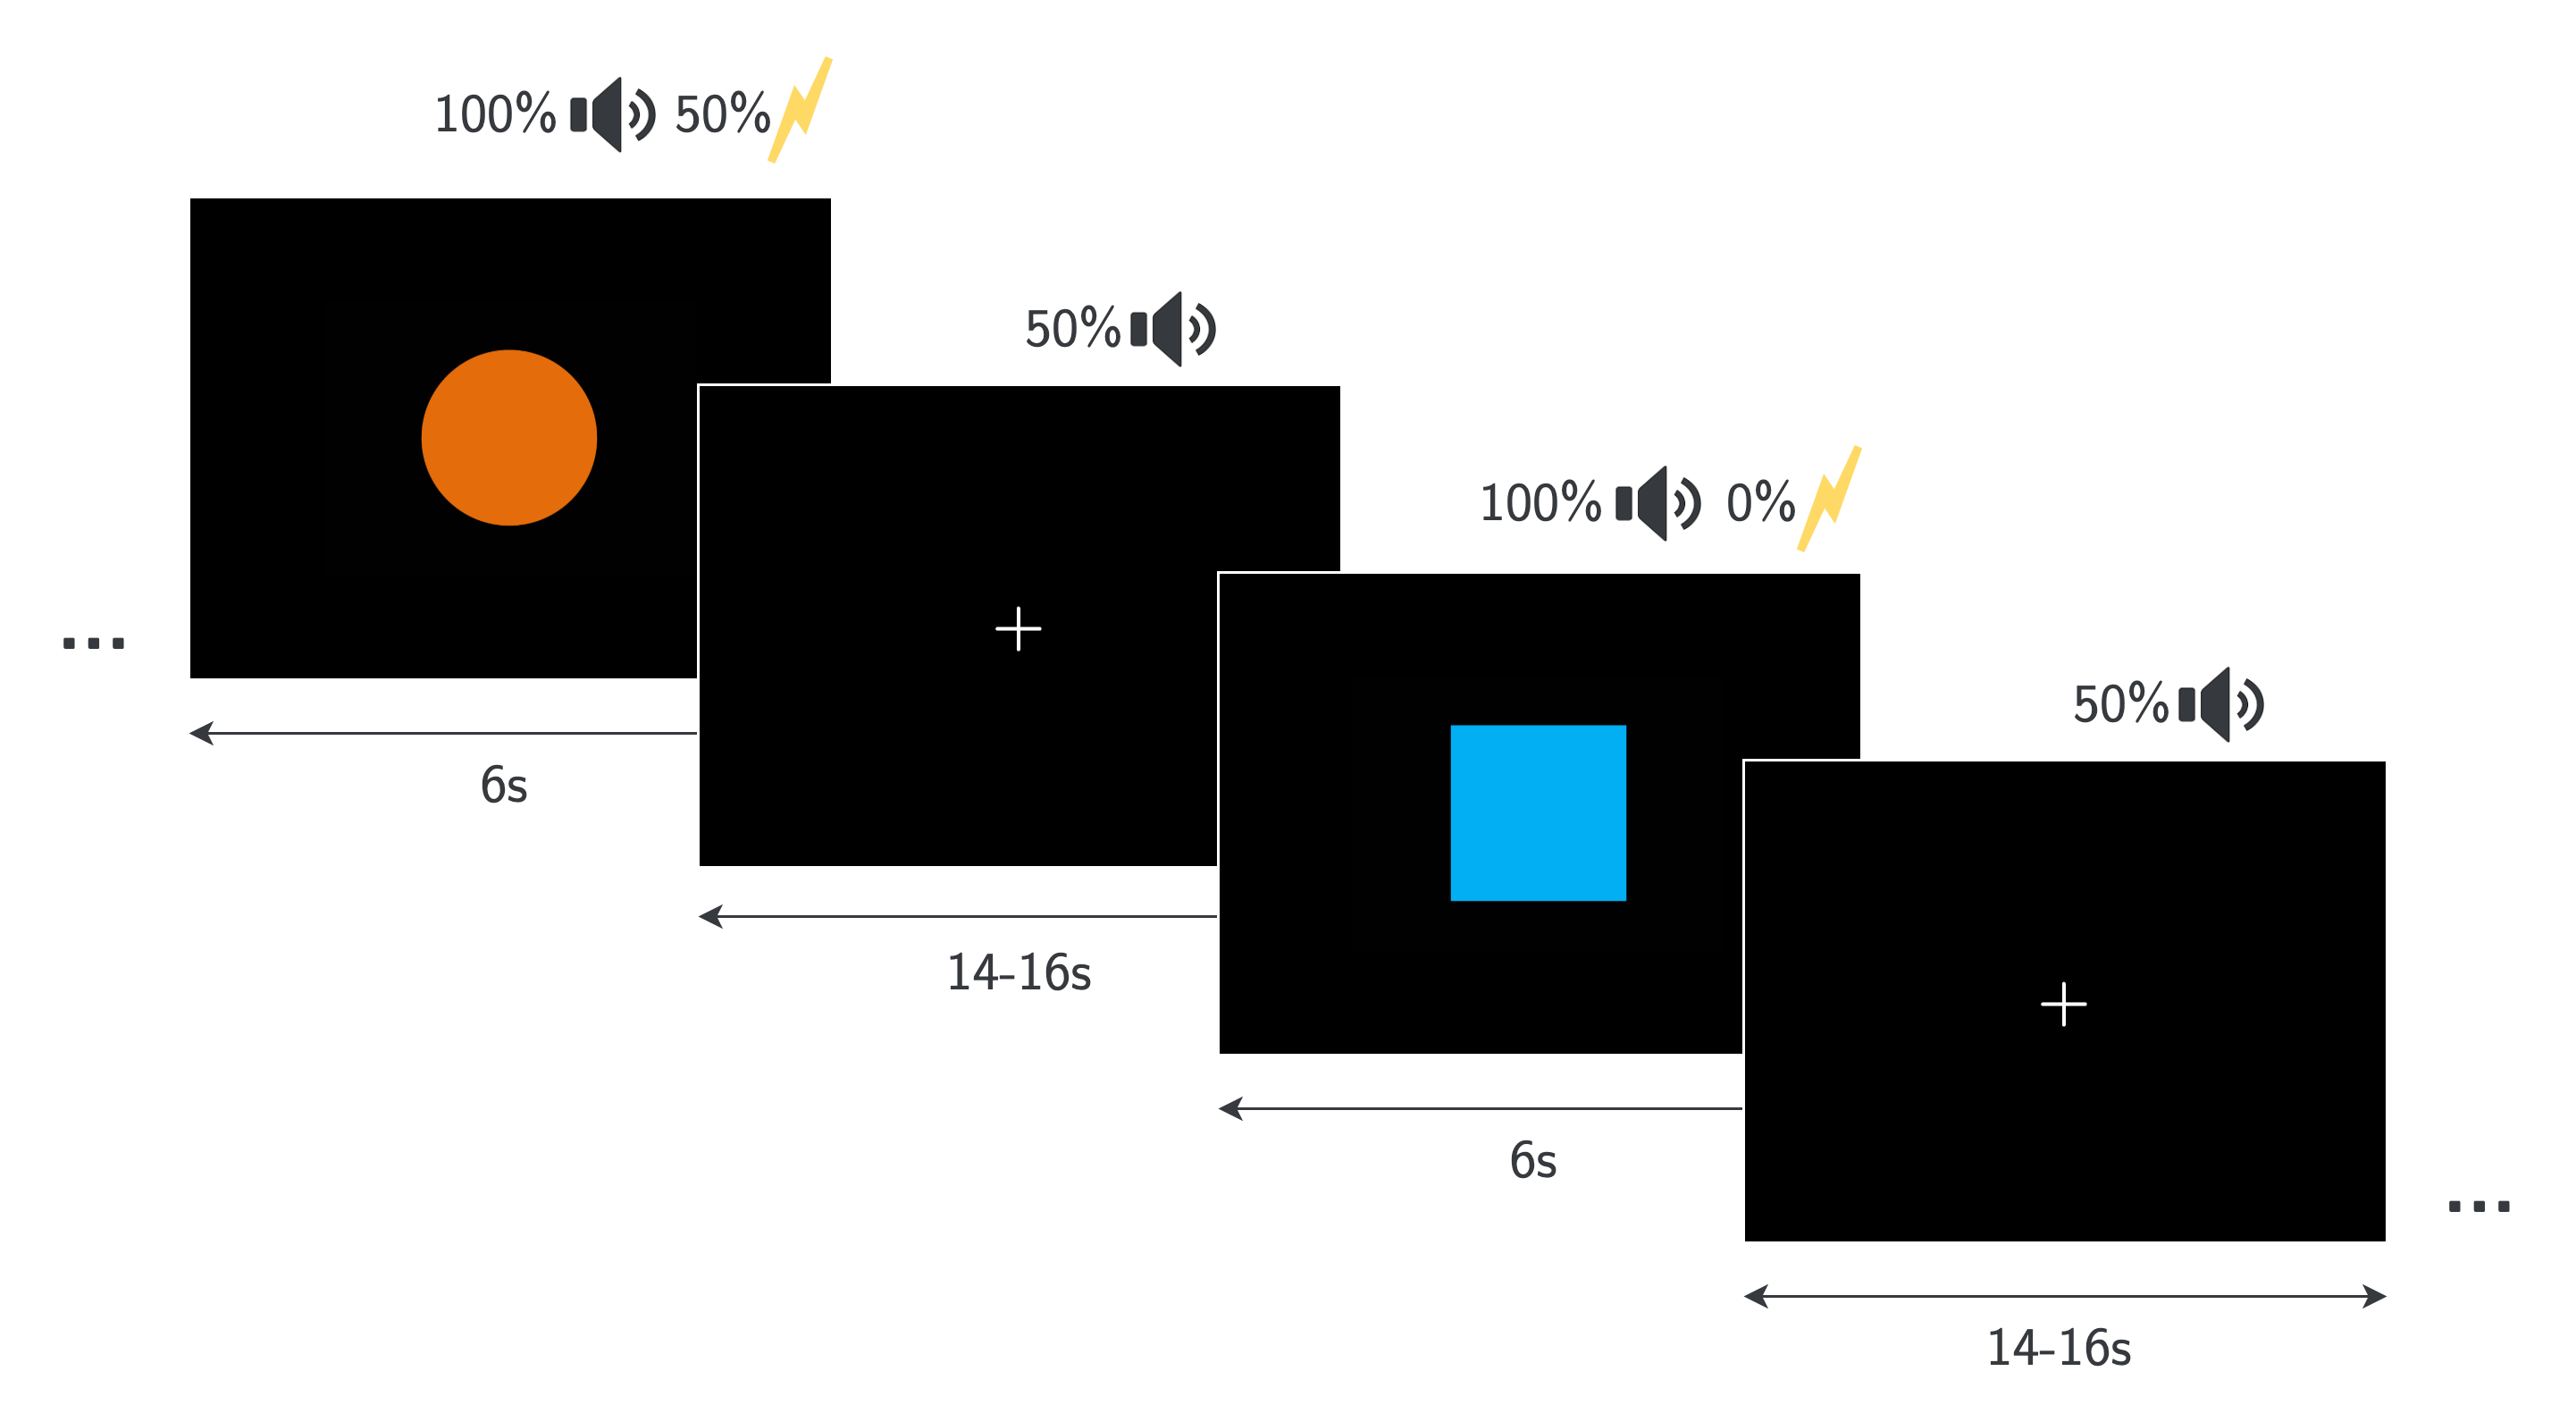
\includegraphics[width=0.9\textwidth]{ablauf.png}
					 			\caption[Schematischer Ablauf der Trials]{Schematischer Ablauf der Trials (exemplarisch: orangener Kreis als CS+). Die Prozente entsprechen den Wahrscheinlichkeiten für die Vergabe von Schreckreizen und elektrotaktilen Reizen in den jeweiligen Trials.}
					 			\label{fig:ablauf}
					 	\end{center}\end{figure}
				 	
						Die Versuchspersonen werden auf jeweils einer von vier verschiedenen Trialreihenfolgen getestet, deren wesentliche Unterschiede darin liegen, mit welchen Stimuli das Akquisitionstraining beginnt (CS+ oder CS--) und ob der erste präsentierte CS+ verstärkt wird oder nicht. Die Reihenfolgen werden über Versuchspersonen hinweg ausbalanciert. 
						In der Hälfte des Trainings nach dem $16.$ Trial wird eine vollständige Instruktion auf dem Bildschirm präsentiert. Mit dem Wortlaut "`Wenn ein unangenehmer Reiz am Bein erfolgt, dann immer nur bei diesem Symbol:"' und einer Abbildung des CS+ werden die Versuchspersonen über die CS-US-Kontingenz aufgeklärt.
						Grund für die Darbietung der Instruktion ist einerseits die Fokussierung des Großprojekts auf den Extinktionstermin, für den eine gelernte CS-US-Kontingenz unabdingbar ist, und andererseits die anteilige Messung der Patient*innen-Stichprobe.
						
					%POST- FURCHTAKQUISITIONSTRAINING
						Das Akquisitionstraining insgesamt dauert ca. \SI{12}{\minute}. Im Anschluss werden die Proband*innen erneut um eine Einschätzung aller präsentierten Reize (CS+, CS--, Auslösereiz, US) auf den SAM-Skalen (\nameref{appB}) gebeten. Es folgt ein kurzes Bewusstseins-Interview, bei dem erfasst wird, ob die Versuchspersonen eine Regel in Bezug auf die CS-US-Kontingenz verbalisieren können. An dieser Stelle wird von der Versuchsleitung sichergestellt, dass die Kontingenz spätestens nach Abschluss des Trainings bekannt ist. Dieses halb-standardisierte Interview soll eine erfolgreiche Furchtakquisition bei allen Versuchspersonen gewährleisten, um den für das Großprojekt relevanten Extinktionstermin durchführen zu können. 
						Nach einigen kurzen Fragen zu Mahlzeiten, Koffein- und Alkoholkonsum vor der Messung werden die Versuchspersonen an die Interventionsleitung übergeben. Dort werden sie über ihre Zugehörigkeit zu Kontroll- bzw. Interventionsgruppe aufgeklärt und im Zuge des Großprojekts weiter begleitet.
					 

%%%%%%%%%%%%%%%%%%%%%%%%%%%%%%%%%%%%%%%%%%%%%%%%
%%%%%%%%%%%%%%%PREPROCESSING%%%%%%%%%%%%%%%%%%%%
%%%%%%%%%%%%%%%%%%%%%%%%%%%%%%%%%%%%%%%%%%%%%%%%

	\section{Datenverarbeitung und Reaktionsdefinition}\label{dataprocessing}

		\subsection{Hautleitwertreaktion}\label{edascore}
			
			Die Vorverarbeitung sowohl der EDA- als auch der EMG-Daten erfolgt in \citeauthor{MATLAB} (Version R2020b, MathWorks, Inc., Natick, USA).	
			Die EDA-Daten werden offline auf \SI{100}{\hertz} heruntergetaktet. Die Vorverarbeitung und Kennwertbestimmung der Daten erfolgt mit der Ledalab Software V3.4.9 \parencite{BENEDEK2010} nach veröffentlichten Richtlinien \parencite{BOUCSEIN2012}. Dabei wird automatisch im Zeitfenster von $0.9$ bis \SI{5}{\second} nach CS-Onset eine klassische Tiefpunkt-bis-Hochpunkt Differenz gebildet, wobei eine Mindestamplitude von \SI{0.001}{\micro\siemens} als Wertungskriterium dient. Die Hautleitwertreaktion entspricht damit der jeweiligen Amplitudenhöhe in~\si{\micro\siemens}. Dadurch, dass der Schreckreiz frühestens \SI{4.5}{\second} nach CS-Onset präsentiert wird und eine SCR auf diesen erst eine Sekunde ihren  Onset hätte, interferiert die Vergabe des Schreckreizes nicht mit der Erfassung der SCR in diesem Zeitfenster.
			Nach der Verarbeitung in Ledalab werden die Gesamtreaktionen der einzelnen Versuchspersonen manuell inspiziert. In $n=2$ Fällen sind keine SCR-Reaktionen im Akquisitionstraining erfasst worden, vermutlich aufgrund des Ablösens der Elektroden während der Messung. Diese beiden Versuchspersonen werden aus allen Folgeanalysen ausgeschlossen.
			Nullreaktionen werden vergeben, wenn die Amplitude der SCR das Mindestkriterium nicht erfüllt. Die übrigen $38$ Datensätze enthalten \SI{18}{\percent} ($223$ von $1\,216$) Nullreaktionen. Fehlende Reaktionen gibt es aufgrund der automatischen Auswertung nicht.
			Auf Basis der Empfehlung eines durchgeführten Box-Cox-Tests für die SCR-Daten wird eine log-Transformation dieser Daten vorgenommen \parencite{BOX1964}.
			%Ledalab Optimizer Nr. 4 (Number of different sets of initial values) einbringen?
			%19.03. finale Analyse: Downsample Faktor 20, Time-Window 0.9-5, Kriterium: 0.001µS, 
		
		\subsection{Schreckreaktion}\label{emgscore}
				
			Die EMG-Daten werden offline in \citeauthor{MATLAB} durch einen Hochpassfilter mit \SI{60}{\hertz} und einen Tiefpassfilter mit \SI{400}{\hertz} geschickt (Butterworth Filter zweiten Grades, \nptextcite{BLUMENTHAL2005}) %60Hz Hochpassfilter, 400Hz Tiefpassfilter --> %alternativ: Breitbandfilter mit Grenzen 60 und 400?
			und durchlaufen zusätzlich einen Kerbfilter bei \SI{50}{\hertz}, um Interferenzen durch Netzbrummen zu reduzieren. % 50Hz Bandstop Filter
			Das Signal wird gleichgerichtet und mit einem Tiefpassfilter von \SI{15.9}{\hertz} und einer Zeitkonstante von \SI{10}{\milli\second} geglättet. %OrbicularisRect= abs(OrbicularisFilt) und OrbicularisIntegratedDef= filter(tp10ms,OrbicularisRect)
			Die Kennwertbestimmung erfolgt manuell, indem innerhalb von $20$ bis \SI{120}{\milli\second} nach dem Schreckreiz der Fußpunkt der Reaktion und innerhalb von \SI{150}{\milli\second} das lokale Maximum als Spitze festgelegt werden \parencite{BLUMENTHAL2005}. Die Schreckreaktion ergibt sich aus der Differenz (d.\,h. der Amplitudenhöhe) in~\si{\micro\volt}.
			Trials, die eine exzessive Grundlinienaktivität oder ein zufälliges Blinzeln kurz vor oder zu Beginn des interessierenden Zeitfensters zeigen, werden als \textit{fehlend}  definiert. Von allen Trials sind $13$ (\SI{1.1}{\percent}) fehlend (wobei keine Versuchsperson mehr als zwei fehlende Werte aufweist). 
			Für Trials, in denen eine Reaktion nicht distinkt erkennbar ist bzw. vollständig ausbleibt, wird eine Nullreaktion vergeben. Die Anzahl der Nullreaktionen beläuft sich auf $19$ (\SI{1.6}{\percent}), wobei anzumerken ist, dass kein Kriterium für eine Mindestreaktionshöhe einer vorhandenen Reaktion angelegt wird.
			%Der Mittelwert und die Standardabweichung der Schreckreaktionen innerhalb der Versuchspersonen wurden berechnet und die Schreckreaktionen anhand dieser Werte z-standardisiert. 
	
	
%%%%%%%%%%%%%%%%%%%%%%%%%%%%%%%%%%%%%%%%%%%%%%%%%%%
%%%%%%%%%%%%%%%STATISTISCHE ANALYSE%%%%%%%%%%%%%%%%
%%%%%%%%%%%%%%%%%%%%%%%%%%%%%%%%%%%%%%%%%%%%%%%%%%%
\section{Statistische Analyse}\label{statistik}
	
	\subsection{Multivariates Wachstumsmodell mit Mehrebenenstruktur}
		Der statistische Vergleich findet durch ein multivariates Wachstumsmodell (engl.: Growth Curve Analysis) im Rahmen eines Mehrebenenmodells statt. 
		Mehrebenenmodelle (MEM) haben sich in den letzten Jahren psychophysiologischer Forschung zunehmend durchgesetzt, da sie für messwiederholte Daten als flexibler und präziser gelten. Als Erweiterung der regulären Regression können mit ihnen Daten analysiert werden, denen eine Mehrebenenstruktur zugrunde liegt (man spricht häufig von einer Hierarchie oder Verschachtelung der Daten).
		Im Fall dieser Arbeit besteht die Mehrebenenstruktur darin, dass für jede Versuchsperson eine Vielzahl an Messungen (mehrere Trials) erhoben wird und die einzelnen Beobachtungen einer Person nicht als unabhängig voneinander anzusehen sind.
		 
		Üblicherweise verwendete statistische Verfahren wie die messwiederholte ANOVA oder Regressionen mit Ordinary-Least-Squares Schätzungen (dt.: Methode der kleinsten Quadrate) können für diese Datenstruktur nicht aufkommen und führen zu verfälschten Schätzparametern und Signifikanztests \parencite{NEZLEK2012}. 
		MEM währenddessen erlauben den Regressionsparametern wie dem Intercept (dt.: Achsenabschnitt) und den Slopes (dt.: Steigungen) zwischen den Ebenen zu variieren. Damit schätzen sie Regressionskoeffizienten nicht nur als feste Effekte (engl.: fixed effects), sondern modellieren sie als zufällige Effekte (engl.: random effects). Die festen Effekte sind ähnlich wie in herkömmlichen Regressionsmethoden zu verstehen.
		Mit der zusätzlichen Schätzung der Zufallsfehler dieser festen Koeffizienten ist es den Regressionsparametern der einzelnen Personen im Modell nun aber \textit{erlaubt}, von diesem mittleren Effekt abzuweichen. Die Modellierung als zufällige Effekte repräsentiert die Annahme, dass die geschätzten Regressionsparameter Stichproben aus einer zugrundeliegenden Verteilung von Parametern in der Grundgesamtheit sind.
		Die simultane Schätzung von Zufallsfehlern nicht nur auf Ebene der Reaktion (Ebene 1), sondern auch auf Ebene der einzelnen Versuchsperson (Ebene 2) ist ein wesentlicher Vorteil von MEM. Vor allem in der Psychophysiologie, wo es zwischen verschiedenen Personen zu enormen Schwankungen in Reaktionsmustern kommen kann, zeigen MEM die notwendige Flexibilität, bessere Erklärungen für ihre Datenmuster bereitstellen zu können.
		Zusätzlich bieten MEM den Vorteil, für eine fehlende Äquidistanz von Messzeitpunkten aufzukommen sowie mit fehlenden Datenpunkten umzugehen (ungleich üblicher ANOVA-Methoden) und damit reliablere Schlussfolgerungen zu liefern. 	
		
		Im Kontext von messwiederholten Daten, denen eine zeitliche Struktur zugrunde liegt, erlauben diese Modelle die Schätzung von sogenannten \textit{Wachstumskurven}. Dieser eher breite Term umfasst im MEM-Kontext die Untersuchung von intraindividuellen Veränderungen und den Prädiktoren, die diese beeinflussen können \parencite{CURRAN2010}.
		Eine tiefgehende Erläuterung der Konzepte von Wachstumskurven- und Mehrebenenanalysen geht über den Umfang dieser Arbeit weit hinaus. Eine englischsprachige Einführung in die Thematik geben zum Beispiel \textcite{BAGIELLA2000, NEZLEK2012} und \textcite{PAGEGOULD2016}, als deutschsprachige Einführung eignet sich \textcite{NEZLEK2006}. Für einen tieferen Einblick seien die Bücher von \textcite{GRIMM2017, BICKEL2007} und \textcite{RAUDENBUSH2002} empfohlen. 
		Um einen Vergleich zweier abhängiger Variablen zu implementieren, wird das univariate Wachstumsmodell auf ein multivariates erweitert \parencite[nach dem Vorbild von][]{CURRAN2012, MACCALLUM1997}. 
		Zusätzlich zu der Schätzung von Wachstumsmodellen für jede der beiden abhängigen Variablen erlaubt der multivariate Ansatz die Untersuchung ihrer Kovarianzen. 
		%Hier kann für jeden der Prädiktoren einzeln der Einfluss auf die Anpassungsgüte geschätzt werden und das wiederum separat für jede der abhängigen Variablen.
		Im Folgenden erläutere ich die in dieser Arbeit umgesetzte Modellstruktur sowie das allgemeine Vorgehen, die Annahmen und die Entscheidungskriterien zum Aufstellen und Schätzen des Modells.
		

	\subsection{Modellstruktur \& Variablen}
		
		Die Daten werden als Zwei-Ebenen-Modell analysiert mit der Reaktion auf Ebene 1 und der Versuchsperson auf Ebene 2. Das heißt, dass jede Reaktion der Versuchsperson zugeordnet wird, von der sie stammt. 
		%Für jede dieser Versuchspersonen wird damit ein individuelles Wachstumsmodell geschätzt für jede der abhängigen Variablen separat und zusätzlich der Einfluss des Stimulustyps und seiner Interaktion mit der Zeit untersucht.
		Einen Überblick über die Datenstruktur liefert Abbildung \ref{fig:struktur}.
		
		\begin{figure}[h]
			\begin{center}
				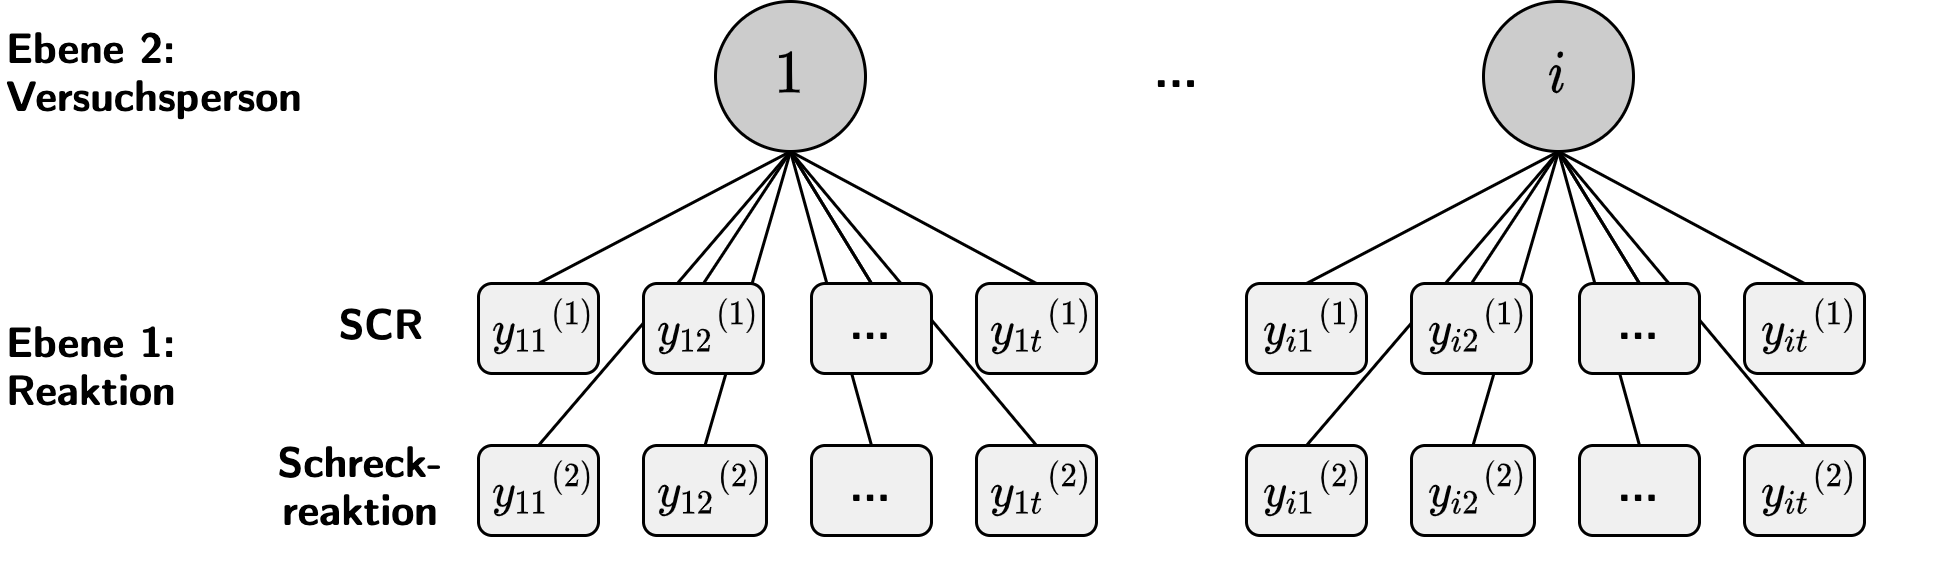
\includegraphics[width=0.8\textwidth]{structure.png}
				\caption[Schematische Datenstruktur im Rahmen des Mehrebenenmodells]
				{Schematische Datenstruktur im Rahmen des Mehrebenenmodells mit zwei Ebenen und zwei abhängigen Variablen ($i$: Versuchsperson, $t$: Trial).}
				\label{fig:struktur}
		\end{center}\end{figure}

		Um ein Wachstumsmodell aufzustellen, benötigt es eine Zeitvariable. In dieser Arbeit wird die Trialnummer als kontinuierlicher Prädiktor herangezogen, um Veränderungen über die Zeit zu erfassen. Bei der Modellbildung wird getestet, ob das Datenmuster der beiden Reaktionsvariablen durch eine lineare oder eine quadratische Zeitvariable besser erklärt werden kann. Dafür wird im Modell ein Polynom-Term zweiten Grades linear-additiv in das Modell inkludiert und sein Effekt auf die Anpassungsgüte überprüft. 
		Um der Multikollinearität der Zeitprädiktoren vorzubeugen, wird die Trialnummer zentriert und anschließend für den quadratischen Modellterm quadriert. Damit liegt der Mittelpunkt der Trialvariable zwischen dem 8. und 9. Trial \parencite[analog zu][]{KRISTJANSSON2007}.
		Der Stimulustyp wird als zweistufiger kategorialer Prädiktor dummykodiert mit dem CS-- als Referenzkategorie. Da jede Versuchsperson sowohl auf den CS+ als auch auf den CS-- in beiden Reaktionsmaßen reagiert, gilt der Stimulustyp als ein sogenannter zeitvarianter Prädiktor, der auf Reaktionsebene des Modells hinzugefügt wird.
		Das multivariate Wachstumsmodell enthält schließlich ebenfalls eine Variable, die kodiert, zu welchem Reaktionsmaß eine Reaktion gehört. Es untersucht den individuellen Verlauf der beiden abhängigen Variablen und kann zusätzlich die Kovariationen zwischen den Koeffizienten dieser beiden Wachstumsmodelle schätzen \parencite{GRIMM2017}. Die Besonderheit ist, dass für jede Person ein eigenes Wachstumsmodell für die Hautleitwert- und die Schreckreaktion geschätzt wird, indem die jeweilige Reaktionsvariable in Abhängigkeit von der Zeit und gegebenenfalls vom Stimulustyp bestimmt wird.
		Die Modellbildung erfolgt mit den unstandardisierten Werten beider Variablen. %xxx ggf: 
		%für den Vergleich der Parameter zwischen den Reaktionsvariablen wird das finale Modell zusätzlich einmal mit standardisierten Werten geschätzt, wobei jeweils der Gesamtmittelwert und die Standardabweichung der Werte genutzt werden.
		Die Tabelle \ref{tab:structure} zeigt exemplarisch die Struktur des Datensatzes in langem Format einschließlich der Kodierung und Zentrierung der Prädiktorvariablen.
		\begin{table}[hbt] \small \setstretch{1.5}
			\begin{threeparttable}
				\caption{Exemplarische Datenstruktur}			%ohne Punkt
				\label{tab:structure}
				\begin{tabularx}{\textwidth}{CCCCCCCC}         \toprule	
					VP  & Reihenfolge & Trial & lin  & quad  & CS & AV  & Reaktion \\\hline
					\rowcolor[HTML]{EFEFEF}
					1   & 3     & 1     & -7.5 & 56.25 & 0        & SCR & 0.0059   \\
					1   & 3     & 1     & -7.5 & 56.25 & 0        & STR & 61.421   \\\rowcolor[HTML]{EFEFEF}
					1   & 3     & 1     & -7.5 & 56.25 & 1        & SCR & 1.5482   \\
					1   & 3     & 1     & -7.5 & 56.25 & 1        & STR & 29.184   \\\rowcolor[HTML]{EFEFEF}
					1   & 3     & 2     & -6.5 & 42.25 & 0        & SCR & 0.0024   \\
					1   & 3     & 2     & -6.5 & 42.25 & 0        & STR & 49.147   \\\rowcolor[HTML]{EFEFEF}
					1   & 3     & 2     & -6.5 & 42.25 & 1        & SCR & 0.2949   \\
					... & ...   & ...   & ...  & ...   & ...      & ... & ... \\[-0.2em]\bottomrule 
				\end{tabularx}
				\begin{tablenotes}[normal, flushleft, para]
					\footnotesize{
						\item \textit{Anmerkungen.} VP: Versuchsperson, Reihenfolge: Zuordnung der Trialreihenfolge, lin: linearer zentrierter Zeitterm, quad: quadrierter zentrierter Zeitterm, CS: Stimulustyp (1: CS+, 0: CS--), AV: abhängige Variable (SCR: Hautleitwertreaktion, STR: Schreckreaktion).}
				\end{tablenotes}
			\end{threeparttable}
		\end{table}
		
		\subsection{Allgemeines Vorgehen bei der Modellbildung}
		
		Der Modellbildungsprozess läuft in mehreren Schritten ab. Nach einer deskriptiven und visuellen Analyse der Reaktionsvariablen wird in Schritt 0 zunächst ein unkonditioniertes Modell aufgestellt, welches keinerlei Prädiktoren enthält. Dieses sogenannte \textit{Nullmodell} dient dazu, die Variabilität zu erfassen, die auf Unterschiede der Versuchspersonen zurückgeführt werden kann. 
			\begin{alignat*}{3}
				\text{Ebene 1} &\qquad\qquad& y_{it}{}^{(k)}&=  	\uppi_{0i}{}^{(k)}+e_{it}{}^{(k)}&\qquad\qquad
			%\tag{2}
			\nr\label{eq:null1}\\
				\qquad\text{Ebene 2} && \uppi_{0i}{}^{(k)}&=  \upbeta_{00}{}^{(k)}+r_{0i}{}^{(k)}&\qquad\qquad \notag
			\end{alignat*}
		In diesem Nullmodell ist $y$ die Reaktion der Versuchsperson $i$ zum Zeitpunkt $t$ auf der Reaktionsvariable $k$. Der Index $k$ beschreibt für $k=1$ die Hautleitwertreaktion und für $k=2$ die Schreckreaktion. Der Modellterm $\uppi_{0i}{}^{(k)}$ ist der individuelle Intercept der Person $i$ auf der Variable $k$.
		Das Residuum $e_{it}{}^{(k)}$ erfasst die Abweichung der Reaktion $y$ vom individuellen Mittelwert, wiederum jeweils für beide $k$. 
		Ebene~2 enthält die Gleichung, mit der der Intercept als zufälliger Effekt modelliert wird. Das Residuum $r_{0i}{}^{(k)}$ gibt an, wie der personenspezifische Intercept vom globalen (festen) Intercept $\upbeta_{00}{}^{(k)}$ abweicht.
		Diese Mehrebenengleichungen lassen sich auch in einem gemischten Format (d.\,h. innerhalb einer Gleichung für beide abhängigen Variablen) kombinieren. Um das zu realisieren, werden zwei zusätzliche Dummyvariablen benötigt – eine für jedes Reaktionsmaß. Diese kodieren, zu welcher abhängigen Variable eine Reaktion zugeordnet werden kann \parencite{MACCALLUM1997}.
		\begin{align*}		
			\updelta_1 = \begin{cases}
				1  & \text{ wenn } k=1 \text{ (Hautleitwertreaktion)}\\
				0  & \text{ wenn } k=2 \end{cases} 
			\qquad \text{und} \qquad \updelta_2 = \begin{cases}
				1  & \text{ wenn } k=2 \text{ (Schreckreaktion)}\\
				0  & \text{ wenn } k=1\end{cases} \nr\label{eq:delta}
		\end{align*}
		Mit der Wichtung über die Dummyvariablen ist es möglich, ein einziges Modell zu schätzen und dabei separate Wachstumsmodelle für die jeweiligen Reaktionsmaße sowie ihre geteilte Varianz zu bestimmen. Dabei kann das Modell trotz einer multivariaten Zwei-Ebenen-Struktur mit derselben Linearkombination geschätzt werden. Für ein gegebenes $y_{it}{}^{(1)}$ zum Beispiel gewährleistet die Variable $\delta$, dass der zweite Summand der Summe aus der Gleichung \eqref{eq:null2} entfällt. In der Summenschreibweise werden damit für  $m=1$ die Regressionsparameter der Hautleitwertreaktion ($k=1$) und für $m=2$ die der Schreckreaktion ($k=2$) geschätzt.
		\begin{equation*}
			y_{it}{}^{(k)}=\sum^2_{m=1} \updelta_m \left( \upbeta_{00}{}^{(m)}+ 		
			r_{0i}{}^{(m)}+e_{it}{}^{(m)}\right)\nr\label{eq:null2}
		\end{equation*}
	
		In Schritt 1 wird die Struktur der zufälligen Effekte bestehend aus zufälligen Intercepts und Slopes für jedes Reaktionsmaß festgelegt. 
		Dafür wird zunächst die maximale Struktur festgestellt (d.h. jeder Regressionskoeffizient wird als zufällig modelliert; \nptextcite{BARR2013}).
		In der maximalen Struktur sind neben zufälligen Intercepts außerdem zufällige Slopes für beide Zeitterme, den Stimulustyp und seine Interaktionen mit den Zeittermen enthalten \parencite{BRAUER2018}.
		Außerdem schätzt das Modell die Kovarianzen zwischen den einzelnen Effekten.
		Es kann vorkommen, dass das Modell für die Datengrundlage, auf der es beruht, zu komplex ist. Dann können Konvergenzprobleme oder sehr hohe Korrelationen zwischen den zufälligen Effekten auftreten \parencite{BRAUER2018, MATUSCHEK2017}.
		Sind zufällige Effekte nah bei null, kann das bedeuten, dass zu wenig Varianz in den Daten vorliegt, um diese zu schätzen. Sehr hohe Korrelationen können eine Überanpassung anzeigen.
		In diesen Fällen -- und ebenso bei Konvergenzproblemen -- wird empfohlen, die Komplexität zu verringern \parencite{BRAUER2018, MATUSCHEK2017}. 
		\textcite{BRAUER2018} stellen in ihrem Artikel einen Leitfaden für diesen Zweck zur Verfügung. Sollte einer der genannten Fälle bei der maximalen Struktur zufälliger Effekte auftreten, werden die Empfehlungen von \textcite{BRAUER2018} zu Rate gezogen. Im Ergebnisteil werden die auf deren Basis getroffene Entscheidungen ausführlich dargelegt. Potentielle Schritte zur Behebung umfassen das Heraufsetzen der maximalen Iterationen, das Herausnehmen bestimmter -- potentiell weniger relevanter -- zufälliger Effekte oder das Unterdrücken von Kovarianzen zwischen ihnen \parencite{BARR2013, BRAUER2018}. 
	 	Modelle mit verschiedenen zufälligen Effekten werden über das Restricted Maximum-Likelihood (REML) Verfahren berechnet, da es präziser für die Schätzung der Varianzkomponenten ist \parencite[für eine Gegenüberstellung von ML und REML siehe][]{RAUDENBUSH2002}.
		
	
		Ist die Struktur der zufälligen Effekte gewählt, kann in Schritt 2 die passende Struktur der Zeitterme für die Daten gewählt werden. 
		Diese festen Effekte werden sequentiell über Vorwärtsselektion hinzugefügt und ihr Einfluss auf die Anpassungsgüte mittels Modellvergleichen -- in diesem Fall Likelihood-Ratio Tests (LRT) -- evaluiert. Der LRT vergleicht ein einfacheres Modell %(hier $M1$) 
		mit einem komplexeren. Die Nullhypothese, dass die Anpassungsgüte der beiden Modelle keinen Unterschied aufweist, wird abgelehnt, wenn die $\upchi^2$-verteilte Teststatistik
		%$$\upchi^2_{df(M2)-df(M1)}= 2\,\left(\text{logL}_{M2}-\text{logL}_{M1}\right)$$
		auf einem \SI{5}{\percent}-Niveau signifikant wird. Eine bedeutend bessere Anpassung des komplexeren Modells resultiert in seiner Weiterverwendung. Bei einer Insignifikanz wird das sparsamere Modell beibehalten.	
		Zusätzlich liefert das R-Paket \texttt{nlme} approximierte $p$-Werte und Konfidenzintervalle für feste Effekte auf Basis von bedingten $t$-Tests \parencite{PINHEIRO2000}. Beim Auswählen der Struktur der festen Effekte präferieren \textcite{PINHEIRO2000} die Verwendung der $p$-Werte über LRT-Vergleiche. In dieser Arbeit ziehe ich beide Verfahren zur Beurteilung der Signifikanz heran. Sollte das Signifikanzergebnis unterschiedlich sein, wird das Ergebnis des $t$-Tests priorisiert.
		Ausgehend von dem Nullmodell mit der zufälligen Effekt-Struktur aus Schritt 1 wird zunächst der lineare Zeitterm (lin) als Prädiktor hinzugefügt. Mit Aufnahme des quadrierten Terms (quad) wird getestet, welche Zeitstruktur eine bessere Anpassungsgüte an die Daten aufweist. Beim Vergleich von Modellen mit unterschiedlicher Struktur der festen Effekte werden die Parameter iterativ mit dem Maximum-Likelihood (ML) Verfahren geschätzt. 
		
		Sobald auch die Struktur der Zeitterme ausgewählt ist, kann der zeitvariante Prädiktor Stimulustyp in das Modell aufgenommen werden. In Schritt 3 wird diese Variable auf Ebene 1 eingefügt. Mittels LRT wird separat für jede der abhängigen Variablen überprüft, ob die Interaktion von Stimulustyp mit den Zeittermen zu einer besseren Anpassungsgüte führt. Ist diese Verbesserung signifikant, erhält das komplexere Modell den Vorzug. Für die Vergleiche von Modellen mit unterschiedlicher fester Effekt-Struktur wird erneut das ML-Schätzverfahren verwendet.
		
		Das maximal mögliche Modell enthält für jede der abhängigen Variablen einen linearen (lin) und einen quadratischen Zeitterm (quad) sowie den Prädiktor Stimulustyp (CS) und seine Interaktionen mit den Zeittermen. Die zufällige Effekt-Struktur ist maximal, d.\,h. dass jeder Regressionskoeffizient als zufällig modelliert wird.
		\begin{align*}
			y_{it}{}^{(k)}= \sum_{m=1}^{2}\, \updelta_m \,&
			\left[ \left( 
				\upbeta_{00}{ }^{(m)} + 
				\upbeta_{10}{ }^{(m)}\, \text{lin}_{it} + 
				\upbeta_{20}{ }^{(m)}\, \text{quad}_{it}+
				\upbeta_{30}{ }^{(m)}\, \text{CS}_{it}
			\right. \right. \nr \label{eq:full1} \\
			&\qquad +\left.  
				\upbeta_{40}{ }^{(m)}\, \text{lin}_{it}\,\text{CS}_{it} + 
				\upbeta_{50}{ }^{(m)}\, \text{quad}_{it}\,\text{CS}_{it} 
			\right)\\
			&\qquad +
			\left( 
				r_{0i}{ }^{(m)} + 
				r_{1i}{ }^{(m)}\, \text{lin}_{it} + 
				r_{2i}{ }^{(m)}\, \text{quad}_{it} + 
				r_{3i}{ }^{(m)}\, \text{CS}_{it} \right.\\
			&\qquad +\left.\left.
				r_{4i}{ }^{(m)}\, \text{lin}_{it}\,\text{CS}_{it} + 
				r_{5i}{ }^{(m)}\, \text{quad}_{it}\,\text{CS}_{it}
				\right)+
				e_{it}{ }^{(m)}
			\right]
		\end{align*}
		Dieses Modell erweitert das Nullmodell in Gleichung \eqref{eq:null2} um zusätzliche Parameter. 
		Die Variable $y$ ist wiederum die Reaktion der Versuchsperson $i$ zum Zeitpunkt $t$ auf Reaktionsvariable $k$. Über die Dummy-Variablen aus Gleichung \eqref{eq:delta} lässt sich die multivariate Form auch hier über eine Summe darstellen, wobei das Modell für $m=1$ Parameter der SCR schätzt und für $m=2$ die der Schreckreaktion. Die Effekte $\upbeta$ werden für jedes Reaktionsmaß $k$ separat berechnet, ebenso die zufälligen Effekte $r$ und der Residuen-Term $e$ auf Ebene~1. Die Prädiktorvariablen variieren über Person $i$ und Messzeitpunkt $t$, allerdings unterscheiden sie sich nicht für die verschiedenen abhängigen Variablen, weswegen diese Modellterme keinen oberen Index haben. 
		Durch die neuen Modellterme beschreibt $\upbeta_{00}$ nun den mittleren Intercept zwischen dem $8.$ und $9.$ CS-- Trial (durch die Zentrierung von Trial und dem CS-- als Referenzkategorie).
		Der Parameter $\upbeta_{10}$ definiert für jedes $k$ die mittlere (momentane) lineare Änderungsrate für den CS--, $\upbeta_{20}$ die mittlere quadratische Slope für den CS--.
		Der mittlere Effekt des Stimulustyps wird durch $\upbeta_{30}$ beschrieben, $\upbeta_{40}$ schätzt den mittleren Unterschied in der linearen Änderungsrate und $\upbeta_{50}$ den mittleren Unterschied in der quadratischen Änderungsrate zwischen CS+ und CS--.
		Die Modellterme $r$ sind die zufälligen Effekte, die die $\upbeta$-Koeffizienten auf Ebene 2 als zufällig modellieren.
		
		Eine vereinfachte Schreibweise bietet die Darstellung über Matrizen (Gleichung \ref{eq:matrix1}).
		Angenommen, $\mat{X}_1$ sei eine Matrix der festen Effekte und $\mat{B}^{(k)}$ eine Matrix der Koeffizienten dieser Effekte für jedes $k$ sowie $\mat{X}_2$ eine Matrix aller als zufällig modellierten Effekte und $\mat{R}^{(k)}$ eine Matrix der zugehörigen Koeffizienten, dann bietet Gleichung \eqref{eq:matrix2} eine minimalistische Schreibweise des maximal möglichen Modells dieser Arbeit aus Gleichung \eqref{eq:full1}.
		\begin{align*}
			\mat{B}^{(k)} = \begin{bmatrix} \upbeta_{00}{}^{(k)} \\ \upbeta_{10}{}^{(k)} \\\upbeta_{20}{}^{(k)}\\\upbeta_{30}{}^{(k)}\\\upbeta_{40}{}^{(k)} \\ \upbeta_{50}{}^{(k)}\end{bmatrix}, \qquad
			\mat{X}_1 = \begin{bmatrix}1\\ \text{lin}_{it}\\ \text{quad}_{it}\\ \text{CS}_{it}\\ \text{CS}_{it}\times\text{lin}_{it}\\ \text{CS}_{it}\times\text{quad}_{it}\end{bmatrix}, \qquad
			\mat{R}^{(k)} = \begin{bmatrix} r_{0i}{}^{(k)} \\ r_{1i}{}^{(k)} \\r_{2i}{}^{(k)}
				\\r_{3i}{}^{(k)}\\r_{4i}{}^{(k)} \\ r_{5i}{}^{(k)}
			\end{bmatrix}, \qquad
			\mat{X}_2 = \begin{bmatrix}1\\ \text{lin}_{it}\\ \text{quad}_{it}
				\\\text{CS}_{it}\\ \text{CS}_{it}\times\text{lin}_{it}\\ \text{CS}_{it}\times\text{quad}_{it}
			\end{bmatrix}
			\nr\label{eq:matrix1}
		\end{align*}

		\begin{align*}
			y_{it}{}^{(k)}= \sum_{m=1}^{2}\, \updelta_m \,\left[ 
			\left(\mat{B}^{(m)}\right)^T\mat{X}_1+
			\left(\mat{R}^{(m)}\right) ^T\mat{X}_2+
			e_{it}{}^{(m)}\right] 
			\nr\label{eq:matrix2}
		\end{align*}
	
%		\begin{align*}
%			y_{it}{}^{(k)}= \sum_{m=1}^{2}\, \updelta_m \,\left[ 
%			\langle \mat{B}^{(m)}, \mat{X}_1 \rangle +
%			\langle \mat{R}^{(m)}, \mat{X}_2 \rangle+
%			e_{it}{}^{(m)}
%			\right] 
%			\nr\label{eq:matrix3}
%		\end{align*}

		%das maximale Modell schätzt 93 Parameter: 12 Fixed Effects (6 each), 12 Random Effects (6 each), 66 Kovarianzen der Random Effects (within and between AV), 2 Residuals (i guess?) plus 1x Kovarianz dieser Residuals
	%TEXTSCHNIPSEL
		%An dieser Stelle fällt auf, dass es der Term $e_{it}$ außerhalb der Summe und damit unabhängig von der Dummyvariable $\delta_k$ auftaucht. Dies ist einer Einschränkung des verwendeten Pakets zur Schätzung geschuldet und bedeutet in diesem Kontext, dass die Residuen auf Ebene der Versuchspersonen ... %XXX
		Im Einklang mit üblichen Konventionen wird das finale multivariate Wachstumsmodell mit dem REML-Verfahren geschätzt und anschließend die Ergebnisse berichtet.
		Alle statistischen Analysen erfolgen in der freien Programmiersprache R für statistische Berechnungen (Version 4.0.3, \citeauthor{R}, \citeyear{R}). Die Modellschätzung erfolgt mit dem Paket \texttt{nlme} \parencite{nlme}. Weitere verwendete Pakete im Zuge der Datenaufbereitung und Visualisierung sind \texttt{tidyverse} \parencite{TIDYVERSE}, \texttt{MASS} \parencite{mass} und \texttt{extrafont} \parencite{EXTRAFONT}. %xxx andere R packages
		
		Die Beantwortung der explorativen Fragestellungen wird lose in zwei Abschnitte geteilt. Zunächst wird über die Modellbildung deutlich, ob bei beiden abhängigen Variablen die gleiche Zeittermstruktur signifikant wird. Hierüber wird ersichtlich, durch welche Wachstumskurven sich die Reaktionsmaße am besten modellieren lassen. 
		Zur Betrachtung des differentiellen Furchtlernens wird untersucht, welchen Einfluss die Interaktionen von Stimulustyp und Zeittermen auf die Anpassungsgüte haben. Durch die Möglichkeit, Effekte als zufällig zu modellieren, können explorativ Aussagen über die Unterschiedlichkeit von Versuchspersonen auf einzelnen Regressionsparametern getroffen werden (in Abhängigkeit von der Modellbildung). Außerdem lassen sich vereinzelt Korrelationen zwischen zufälligen Parametern der abhängigen Variablen prüfen.

	\subsection{Zu prüfende Annahmen}
			Zunächst wird angenommen, dass die Residuen auf Ebene~1 ($e_{it}{}^{(k)}$) multivariat normalverteilt sind mit einem Erwartungswert von $0$. % und der Kovarianzmatrix  $\mat{R}$ %(eine $T\times T$ Kovarianzmatrix, wobei $T$ die Anzahl an wiederholten Messungen ist)
			\begin{equation*}
				\begin{bmatrix}e_{it}{}^{(1)} \\ e_{it}{}^{(2)}\\\end{bmatrix}
				\sim \mathcal{N}
				\left( \begin{bmatrix} 0 \\ 0 \end{bmatrix} ,\, \begin{bmatrix*}[l]
					\upsigma^2_{e^{(1)}} & \\  \upsigma_{e^{(1)},e^{(2)}} & \upsigma^2_{e^{(2)}}
				\end{bmatrix*}\right) 
				\nr\label{eq:assum1}
			\end{equation*}			
			Eine weitere Annahme betrifft die multivariate Normalverteilung der zufälligen Komponenten auf Ebene~2 mit $\mat{\Sigma_T}$ als unstrukturierter Varianz-Kovarianzmatrix.
			\begin{equation*}
				r_{0i}{}^{(k)},\, r_{1i}{}^{(k)},\,r_{2i}{}^{(k)},\,
				%r_{0i}{}^{(2)},\, r_{1i}{}^{(2)},\, r_{2i}{}^{(2)}
				r_{3i}{}^{(k)},\, r_{4i}{}^{(k)},\, r_{5i}{}^{(k)}
				\sim \, \mathcal{N}\left(0,\,\mat{\Sigma_T}\right)
				\nr\label{eq:assum3}
			\end{equation*}	
			An den Best-Practice-Empfehlungen in \textcite{METEYARD2020} orientiert, werden Annahmen über die Residuen am finalen Modell geprüft.
			Die Residuen jeder abhängigen Variable werden auf Linearität und multivariate Normalverteilung untersucht.
			Außerdem werden die Residuen jeder Reaktionsvariable separat auf Homoskedastizität geprüft. 
			Für diese Annahmen werden Q-Q-Diagramme, Histogramme und Streudiagramme zwischen Residuen und angepassten Werten grafisch evaluiert.   
			Eine weitere Annahme von MEM bezieht sich auf die Abwesenheit von Multikollinearität der Prädiktoren. Durch die Zentrierung der Zeitterme und dem Stimulustyp als binäre Variable wird diese Annahme als unverletzt betrachtet.

%%%%%%%%%%%%%LEITFADEN BACHELORARBEIT
		%	Die Verfahrensweisen bei der Datenerhebung, -auswertung und -analyse müssen so dargestellt werden, dass sie für themenfremde Fachleute nachvollziehbar sind. Im Analyseplan erfolgt die Umformung der empirischen in statistische Hypothesen sowie die Beschreibung der Analyseverfahren zu deren Beantwortung.\\
		%
		%	\textbf{Leitfragen: }Ist der Untersuchungsplan für die Fragestellung angemessen? Sind die Variablen nachvollziehbar operationalisiert und beschrieben (z.B. durch Angaben von Gütekriterien und Normen)? Werden mögliche Störfaktoren bei der Planung berücksichtigt? Wird die Durchführung so geschildert, dass eine Replikation der Untersuchung möglich ist? Wird die Stichprobe hinreichend genau beschrieben (z.B. Einschlusskriterien, ausgeschlossene Probanden: Anzahl und Gründe; demographische Angaben)? Ist der Datensatz für die Fragestellung angemessen? Sind bei der Auswertung die statischen Methoden adäquat gemessen an der Fragestellung und gemessen an der Datenqualität? Werden die Voraussetzungen der statistischen Verfahren diskutiert und werden bei Verletzung der Voraussetzungen Alternativen zur Datenanalyse gesehen, werden die statistischen Verfahren also kritisch und gezielt eingesetzt?
			
			\chapter{Ergebnisse}							\label{ergebnisse}
				
%%%%%%%%%%%%%%%%%%%%%%%%%%%%%%%%%%%%%%%%%%%%%
%%%%%%%%%%%%%% DESKRIPTIV %%%%%%%%%%%%%%%%%%%
%%%%%%%%%%%%%%%%%%%%%%%%%%%%%%%%%%%%%%%%%%%%%

	\section{Explorative Datenanalyse}		\label{descriptive}
	
	Der gesamte Mittelwert der log-transformierten Hautleitwertreaktionen in diesem Datensatz beträgt \SI{0.15}{\log\micro\siemens} ($SD=0.26$). Für die Schreckreaktion liegt der Mittelwert bei \SI{67.57}{\micro\volt} ($SD=61.94$).
	Tabelle \ref{tab:descriptive1} beinhaltet eine Übersicht über deskriptive Statistiken über den Verlauf des Akquisitionstrainings separat für beide abhängige Variablen. Eine signifikante CR (d.\,h. auf den CS+ wird bedeutend stärker reagiert als auf den CS--) ist über alle Trials hinweg für die Hautleitwertreaktionen zu beobachten und zeigt sich in den einzelnen Trials $10$ bis $14$ der zweiten Trainingshälfte. Für die Schreckreaktionen sind in Trial $12$ und $13$ die Reaktionen auf den CS+ signifikant von denen auf den CS-- verschieden sowie ebenfalls gemittelt über den Trainingszeitraum. Abbildung \ref{fig:verläufe} zeigt die durchschnittlichen Verläufe beider abhängigen Variablen über die Dauer des Akquisitionstrainings.
	Die Tabelle \ref{tab:descriptive2} zeigt bivariate Unterschiede und Zusammenhänge zwischen den abhängigen Variablen zu allen Messzeitpunkten auf. Die erste Spalte beinhaltet bivariate Korrelationen von Schreck- und Hautleitwertreaktionen (insgesamt und aufgeschlüsselt nach Messzeitpunkten). 
	\begin{table}[bth] \small \setstretch{1.5}
		\begin{threeparttable} 
			\caption{Deskriptive Statistiken \& Mittelwertunterschiede innerhalb beider abhängiger Variablen}			%ohne Punkt
			\label{tab:descriptive1}
			\begin{tabularx}{\textwidth}{lCCCCCC}  \toprule	%@{} eliminiert space zw. 2 Spalten
				\multirow[c]{2}{*}{\begin{tabular}[c]{@{}l@{}} Trial \end{tabular}} & \multicolumn{3}{c}{SCR} & \multicolumn{3}{c}{STR}	\\\cmidrule{2-7}
				& CS+\,\tnote{a}        & CS--\,\tnote{a}  & Differenz\tnote{b}   & CS+\,\tnote{a}       & CS--\,\tnote{a}   & Differenz\tnote{b}  \\\hline
				\rowcolor[HTML]{EFEFEF}
				insg. &$\mathbf{0.18\,(0.28)}$ &$\mathbf{0.12\,(0.23)}$&$\hspace*{+1.35em}\mathbf{0.06^{***}}$& $\mathbf{70.1\,(59.7)}$& $\mathbf{65.1\,(64.0)}$&$\hspace*{+0.9em}\mathbf{5.0^{**}}$   \\
				1  &$0.31\,(0.38)$ &$0.27\,(0.31)$&$0.04$& $93.1\,(61.1)$& $100.4\,(91.8)$ &$\hspace*{-0.85em}-7.3$   \\\rowcolor[HTML]{EFEFEF}
				2  &$0.14\,(0.24)$ &$0.15\,(0.23)$&$\hspace*{-0.85em}-0.01$& $92.0\,(60.6)$& $85.4\,(64.2)$ &$6.6$     \\
				3  &$0.17\,(0.21)$ &$0.15\,(0.21)$&$0.02$& $94.0\,(75.2)$& $80.5\,(60.5)$ &$13.5$      \\ \rowcolor[HTML]{EFEFEF}
				4  &$0.14\,(0.25)$ &$0.11\,(0.21)$&$0.03$& $73.2\,(55.3)$& $76.7\,(61.4)$ &$\hspace*{-0.85em}-3.5$  \\ 
				5  &$0.16\,(0.29)$ &$0.18\,(0.33)$&$\hspace*{-0.85em}-0.02$& $80.7\,(72.5)$& $83.1\,(66.1)$ &$\hspace*{-0.85em}-2.4$  \\ \rowcolor[HTML]{EFEFEF}
				6  &$0.20\,(0.31)$ &$0.18\,(0.29)$&$0.02$& $61.6\,(47.4)$& $70.4\,(75.0)$ &$\hspace*{-0.85em}-8.8$ \\
				7  &$0.08\,(0.12)$ &$0.09\,(0.17)$&$\hspace*{-0.85em}-0.01$& $66.7\,(55.6)$& $68.2\,(63.1)$ &$\hspace*{-0.85em}-1.5$  \\ \rowcolor[HTML]{EFEFEF}
				8  &$0.15\,(0.31)$ &$0.09\,(0.23)$&$0.06$& $68.1\,(56.7)$& $64.2\,(69.3)$ &$3.9$ \\ 
				9  &$0.34\,(0.43)$ &$0.26\,(0.32)$&$0.08$& $86.0\,(77.3)$& $63.2\,(67.3)$ &$\hspace*{-0.45em}22.8$ \\ \rowcolor[HTML]{EFEFEF}
				10 &$0.17\,(0.23)$ &$0.10\,(0.20)$&$\hspace*{+0.45em}0.07^{*}$& $59.1\,(49.1)$& $57.1\,(63.5)$ &$2.0$  \\ 
				11 &$0.19\,(0.26)$ &$0.06\,(0.12)$&$\hspace*{+0.9em}0.13^{**}$& $63.8\,(60.0)$& $54.2\,(56.2)$ &$9.6$ \\ \rowcolor[HTML]{EFEFEF}
				12 &$0.15\,(0.23)$ &$0.05\,(0.10)$&$\hspace*{+0.9em}0.10^{**}$& $69.1\,(60.8)$& $51.4\,(52.1)$ &$17.7^{*}$ \\ 
				13 &$0.18\,(0.28)$ &$0.05\,(0.09)$&$\hspace*{+0.9em}0.13^{**}$& $64.3\,(53.3)$& $44.5\,(38.0)$ &$\hspace*{0.45em}19.8^{**}$  \\\rowcolor[HTML]{EFEFEF}
				14 &$0.24\,(0.33)$ &$0.10\,(0.24)$&$\hspace*{+0.45em}0.14^{*}$& $47.5\,(44.9)$& $47.1\,(48.6)$ &$0.4$\\ 
				15 &$0.12\,(0.21)$ &$0.06\,(0.10)$&$0.06$& $51.7\,(45.6)$& $48.0\,(62.7)$ &$3.7$\\ \rowcolor[HTML]{EFEFEF}
				16 &$0.16\,(0.27)$ &$0.06\,(0.15)$&$0.10$& $50.4\,(49.3)$& $45.4\,(43.9)$ &$5.0$  \\[-0.2em]
				\bottomrule
			\end{tabularx}
			\begin{tablenotes}[normal, flushleft, para]
				\footnotesize{
					\item \textit{Anmerkungen.} SCR: Hautleitwertreaktion, STR: Schreckreaktion, insg.: über alle Trials hinweg.\\
					\item[a] Mittelwerte (für SCR in~\si{\log\micro\siemens}. für STR in~\si{\micro\volt}) mit Standardabweichungen in Klammern.\\
					\item[b] CS+/CS-- Differenzen; Mittelwerte auf Unterschiede getestet mittels gepaarten $t$-Tests; ${}^{*}\, p<.05$, ${}^{**}\, p<.01$, ${}^{***}\, p<.001$.}
			\end{tablenotes}
		\end{threeparttable}
	\end{table}
	Gemittelt über das ganze Training gehen höhere SCR tendenziell mit höheren Schreckreaktionen einher (kleiner Effekt von $r=.13$, $p<.001$). Auch aufgeteilt in einzelne Messzeitpunkte zeigt sich in der Tendenz ein positiver Zusammenhang zwischen den beiden Reaktionsmaßen, auch wenn er nur im ersten ($r=.25$, $p=.03$) und im neunten Trial ($r=.30$, $p=.01$) statistisch bedeutsam ist. In \nameref{appC} ist zusätzlich ein Streudiagramm zwischen den Reaktionen beider abhängiger Variablen zur Visualisierung abgebildet. 
	Die zweite Spalte der Tabelle \ref{tab:descriptive2} zeigt die Korrelationen zwischen den Differenzwerten (CS+ minus CS--) für beide Reaktionsmaße. Der insgesamt kleine, positive Zusammenhang von ($r=.15$, $p<.001$) weist darauf hin, dass eine stärkere konditionierte Reaktion auf dem einen Maß mit einer stärkeren CR auf dem anderen Maß einhergeht. Betrachtet man die einzelnen Trials ist die Korrelation zum Trial $9$ -- direkt nach der Instruktion -- positiv und signifikant ($r=.46$, $p=.004$). In Trial $3$ und $8$ sind die Korrelationen der Differenzwerte signifikant negativ. Hier gehen stärkere CR auf dem einen Maß mit geringeren  CR auf dem anderen Maß einher.
	Die letzte Spalte der bivariaten Tabelle vergleicht die Mittelwerte der CS+/CS-- Differenzen insgesamt und aufgeteilt nach Trials. Dafür wurden die Reaktionen einmalig vorab standardisiert, sodass die Differenzen als $z$-Werte vergleichbar werden. Über das ganze Akquisitionstraining hinweg unterscheiden sich die CS+/CS-- Differenzen für die beiden Maße signifikant voneinander, wobei die $z$-Differenzen der SCR im Durchschnitt größer sind als die der STR. In einzelnen Trials sind diese Unterschiede nur in Trial $14$ evident. Auch hier weist die SCR eine größere Differenz auf.
	
	Eine Überprüfung der Normalverteilung der abhängigen Variablen mittels Shapiro-Wilk-Tests \parencite{SHAPIRO1965} ergab, dass weder global noch für die einzelnen Messzeitpunkte eine Normalverteilung angenommen werden kann (\nameref{appD} liefert eine tabellarische Übersicht der Teststatistiken für beide abhängigen Variablen). Es sei darauf hingewiesen, dass dies nicht einschränkend für die Modellbildung ist. Auf eine Analyse der Ausreißer sowie der fehlenden Werte wird an dieser Stelle verzichtet, da eine Vorverarbeitung im Rahmen der Mehrebenenmodellierung nicht notwendig ist. 
	%Während der Datensatz der SCR aufgrund der automatischen Reaktionsdefinition vollständig ist, beinhaltet der Datensatz der Schreckreaktionen $13$% fehlende Werte. 
	%Eine exemplarische logistische Regression von der binären Variable \textit{fehlt} auf die Prädiktoren Trial, Versuchsperson und Stimulustyp zeigte keine signifikanten Ergebnisse, sodass angenommen werden kann, dass die Werte komplett zufällig fehlen (MCAR, engl. missing completely at random). Für eine Darstellung der Regressionsergebnisse siehe Anhang XXX.

	\begin{figure}[bht]
		\centering
		\begin{tikzpicture}[remember picture] \centering		
			\node[inner sep=0pt] (scr) at (0,0)
			{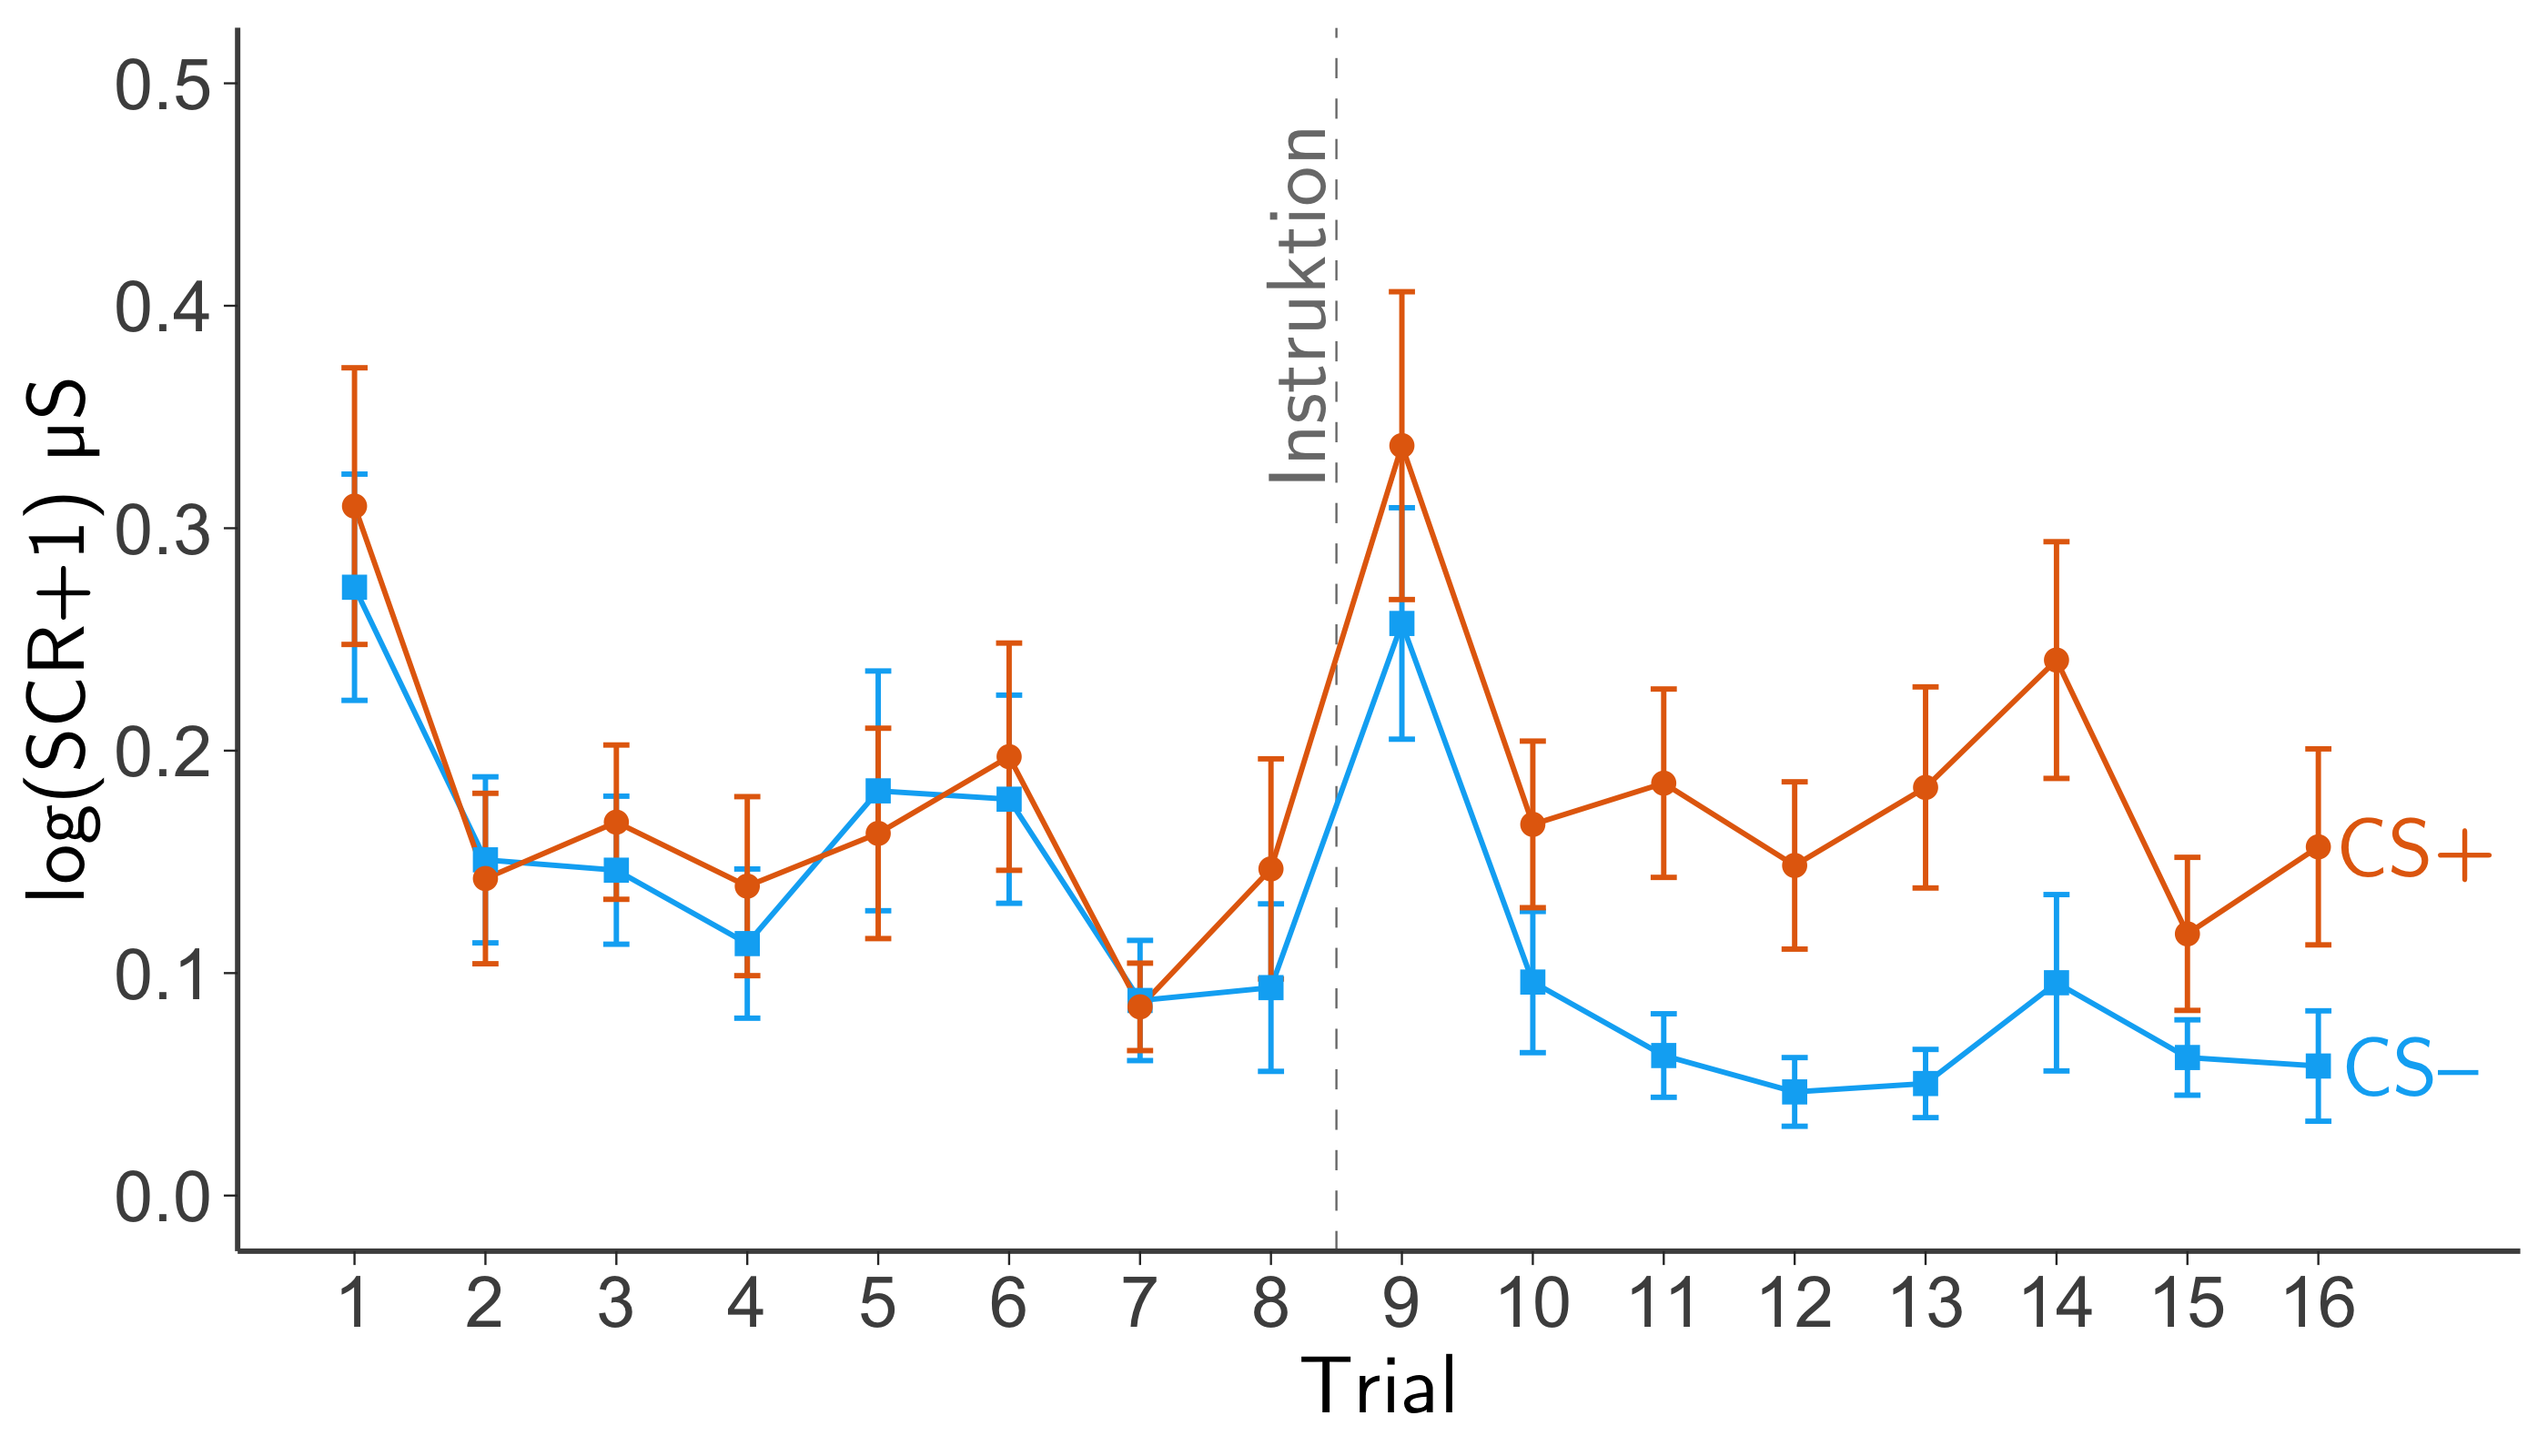
\includegraphics[scale=0.095]{scr_explor2.png}};
			\node[inner sep=0pt, below = 0.5cm of scr] (str)
			{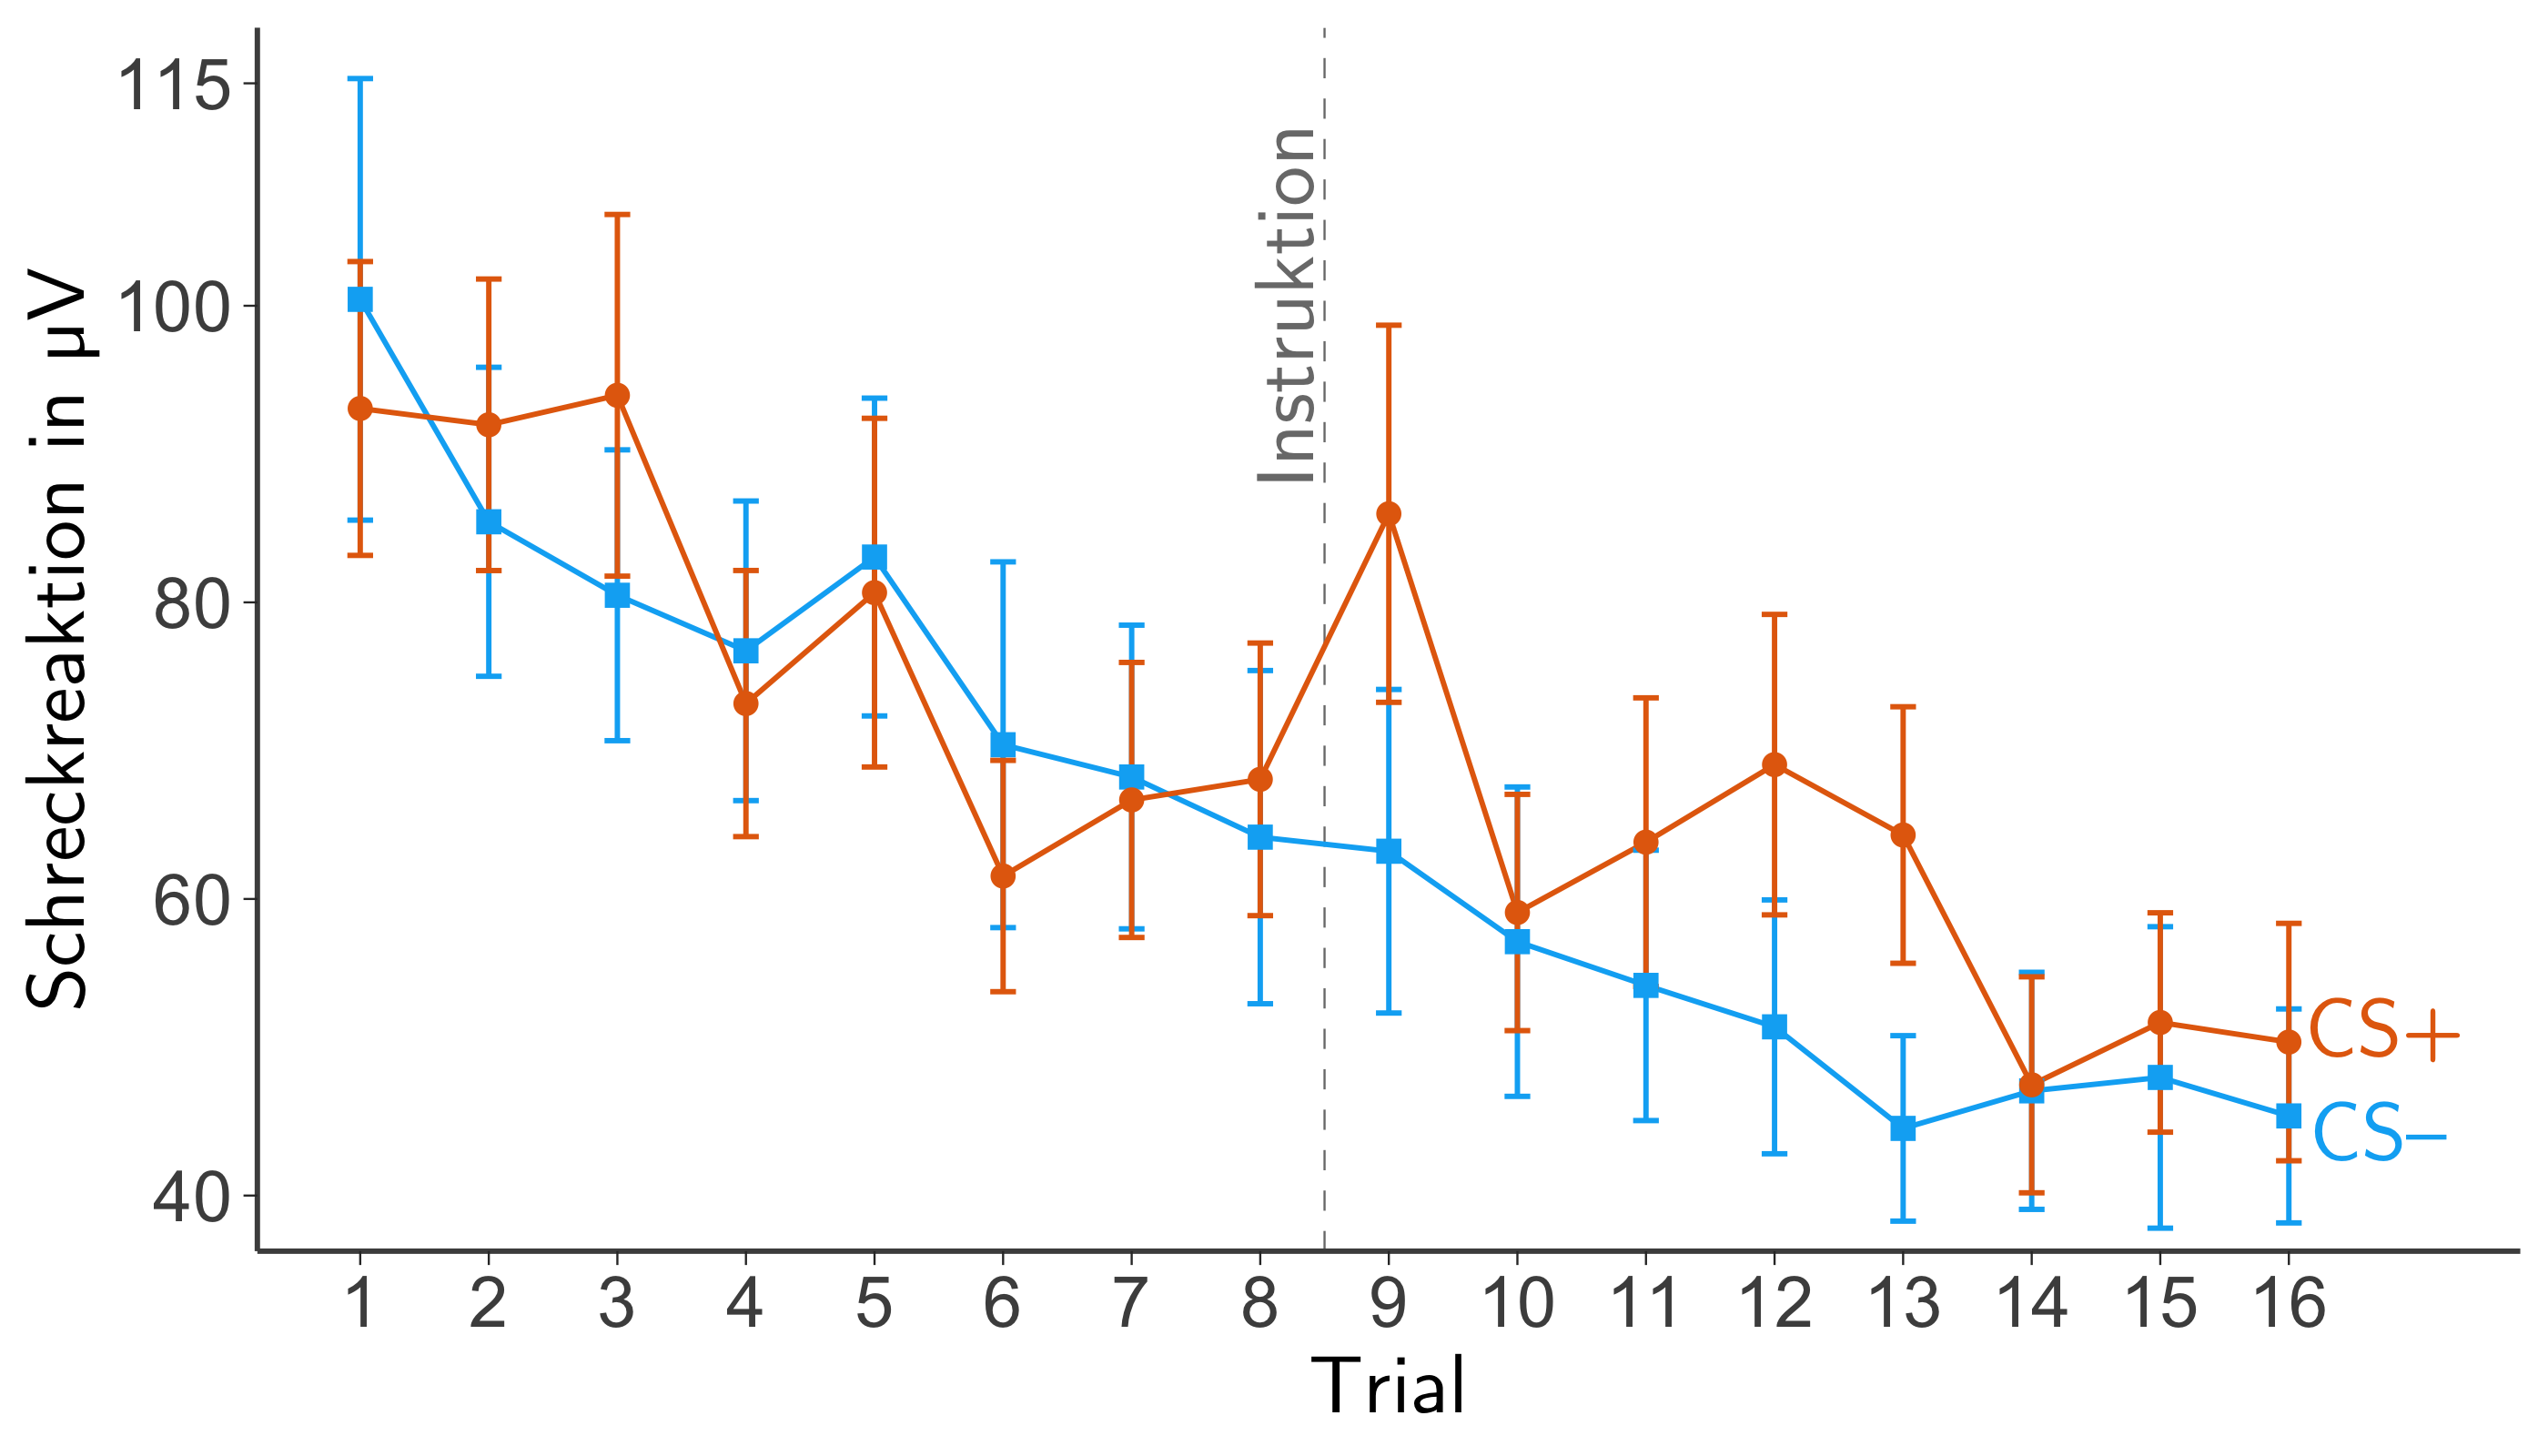
\includegraphics[scale=0.095]{str_explor2.png}};
			\node[above left = 0cm and 0.1cm of scr] (a) {\large{\textsf{\textbf{a}}}};
			\node[above left = 0cm and 0.1cm of str] (b) {\large{\textsf{\textbf{b}}}};
		\end{tikzpicture}
		\caption[Mittlere Verläufe von Hautleitwert- und Schreckreaktionen]{Mittlere Hautleitwert- (\textsf{\textbf{a}}) und Schreckreaktionen (\textsf{\textbf{b}}) auf den CS+ und CS-- über den Verlauf des Experiments. Die Fehlerbalken repräsentieren \textit{SE}.}
		\label{fig:verläufe}
	\end{figure}

	\begin{table}[tb] \small \setstretch{1.5}
	\begin{threeparttable} 
		\caption{Unterschiede \& Zusammenhänge zwischen den abhängigen Variablen}
		\label{tab:descriptive2}
		\begin{tabularx}{\textwidth}{lCCC}  \toprule	%@{} eliminiert space zw. 2 Spalten
			 \begin{tabular}[c]{@{}l@{}} Trial \end{tabular} & \begin{tabular}[c]{@{}c@{}} Korrelation zwischen \\ SCR \& STR \tnote{a}\end{tabular} & \begin{tabular}[c]{@{}c@{}} Korrelation der \\ CS+/CS-- Differenzwerte \tnote{a} \end{tabular} & \begin{tabular}[c]{@{}c@{}}$t$-Teststatistiken der\\  standardisierten Differenzwerte\tnote{b}\end{tabular} \\\hline\rowcolor[HTML]{EFEFEF}
			insg. &$\hspace*{+1.5em}\mathbf{.13^{***}}$&$\hspace*{+1.35em}\mathbf{.15^{***}}$	&$\hspace*{+0.05em}\mathbf{-2.88^{**}}$		\\
			1		&$\hspace*{+0.45em}.25^*$&$.24$		&$\hspace*{-0.85em}-1.01$		 \\\rowcolor[HTML]{EFEFEF}
			2		&$.08$		&$\hspace*{-0.85em}-.08$ 	&$0.77$		 \\
			3		&$.04$		&$\hspace*{-0.45em}-.34^{*}$ &$0.66$		 \\\rowcolor[HTML]{EFEFEF}
			4		&$.01$		&$\hspace*{-0.85em}-.02$ 	&$\hspace*{-0.85em}-0.60$		 \\
			5		&$.09$		&$.28$ 		&$0.18$		 \\\rowcolor[HTML]{EFEFEF}
			6		&$.08$		&$.28$ 		&$\hspace*{-0.85em}-0.94$		 \\
			7		&$.01$		&$\hspace*{-0.85em}-.07$ 	&$\hspace*{-0.85em}-0.22$		 \\\rowcolor[HTML]{EFEFEF}
			8		&$.04$		&$\hspace*{-0.45em}-.36^{*}$ &$\hspace*{-0.85em}-0.84$		 \\
			9		&$\hspace*{+0.9em}.30^{**}$&$\hspace*{+0.9em}.46^{**}$&$0.11$		 \\\rowcolor[HTML]{EFEFEF}
			10		&$.11$		&$.32$ 		&$\hspace*{-0.85em}-1.64$		 \\
			11		&$.06$		&$.00$ 		&$\hspace*{-0.85em}-1.60$		 \\\rowcolor[HTML]{EFEFEF}
			12		&$.16$		&$.18$ 		&$\hspace*{-0.85em}-1.07$		 	\\
			13		&$.14$		&$\hspace*{-0.85em}-.07$ 	&$\hspace*{-0.85em}-0.86$		 \\\rowcolor[HTML]{EFEFEF}
			14		&$.02$		&$.15$ 		&$\hspace*{-0.35em}-2.11^{*}$		 \\
			15		&$.08$		&$.04$ 		&$\hspace*{-0.85em}-0.91$		 \\\rowcolor[HTML]{EFEFEF}
			16		&$\hspace*{-0.85em}-.03$&$.10$ 		&$\hspace*{-0.85em}-1.37$		 \\[-0.2em]\bottomrule
		\end{tabularx}
		\begin{tablenotes}[normal, flushleft, para]
			\footnotesize{
				\item \textit{Anmerkungen.} ${}^{*}\, p<.05$, ${}^{**}\, p<.01$, ${}^{***}\, p<.001$. \item[a] Pearsons Korrelationskoeffizient $r$.	\item[b] Die Reaktionen wurden global $z$-standardisiert ($M=0$, $SD=1$) und die Differenzwerte~CS+/CS-- für SCR und STR gebildet. Diese wurden mit gepaarten~$t$-Tests auf Mittelwertunterschiede geprüft.}
		\end{tablenotes}
	\end{threeparttable}
	\end{table}	

%%%%%%%%%%%%%%%%%%%%%%%%%%%%%%%%%%%%%%%%%%%%%
%%%%%%%%%%%%%%%MODELBILDUNG%%%%%%%%%%%%%%%%%%
%%%%%%%%%%%%%%%%%%%%%%%%%%%%%%%%%%%%%%%%%%%%%

	\section{Modellbildung}		\label{modelbuild}
		Aufgrund der verhältnismäßig kleinen Stichprobengröße und der Komplexität des Modells wird über die Funktion \texttt{lmeControl} \parencite[nach][]{GRIMM2017} in R eine Kontrollfunktion definiert, die unter anderem die maximale Anzahl an Iterationen auf $500$ erhöht.
		Die Konfidenzintervalle und $p$-Werte der Modellparameter werden innerhalb des Pakets \texttt{nlme} über eine Normalapproximation der Verteilung der geschätzten Effekte berechnet \parencite[für die mathematische Herleitung siehe][]{PINHEIRO2000}.
		Eine Übersicht über den im Folgenden beschriebenen sequentiellen Modellbildungsprozess sowie über alle berechneten Modellvergleiche liefert Tabelle \ref{tab:modelbuild}. 
		
		
		\begin{table}[bth] \small \doublespacing
			\begin{threeparttable}
				\caption{Darstellung des Modellbildungsprozesses und der getätigten Modellvergleiche}			%ohne Punkt
				\label{tab:modelbuild}
				\begin{tabularx}{\textwidth}{CllCCccCCC}    \toprule%@{} eliminiert space zwischen zwei Spalten
					&  &  &  &  &  & \multicolumn{2}{c}{Anpassungsgüte} & \multicolumn{2}{c}{LRT} \\ \cmidrule{7-10}
					\multirow[t]{-2}{*}{Schritt} &
					\multirow[t]{-2}{*}{Name} &
					\multirow[t]{-2}{*}{\begin{tabular}[c]{@{}l@{}} einfacheres\\Modell\end{tabular}} &
					\multirow[t]{-2}{*}{\begin{tabular}[c]{@{}l@{}}Feste\\ Effekte\tnote{a}\end{tabular}} &
					\multirow[t]{-2}{*}{\begin{tabular}[c]{@{}l@{}}Zufällige\\ Effekte\tnote{a}\end{tabular}} &
					\multirow[t]{-2}{*}{\begin{tabular}[c]{@{}l@{}}Schätz-\\ methode\end{tabular}} & 
					logL &$df$ & $df$& $\upchi^2$  \\\midrule
					0 & null &  & $\upbeta_{00}{}^{(k)}$  &$r_{0i}{}^{(k)}$ & REML & \multicolumn{1}{l}{$-6079.4$}   & \multicolumn{1}{c}{$7$}  & \multicolumn{1}{c}{--} & \multicolumn{1}{c}{--} \\ 	
					\rowcolor[HTML]{EFEFEF}	
					1 &  ran1 & & \ditto & 
					alle & REML & \multicolumn{4}{c}{\textit{keine Konvergenz erreicht}} \\ 
					1 &  ran2 & & \ditto & $-r_{2i}{}^{(k)}$ & REML & \multicolumn{4}{c}{\textit{keine Konvergenz erreicht}} \\
					\rowcolor[HTML]{EFEFEF}		 
					1 &  ran3 & & \ditto & $-r_{1i}{}^{(k)}$ & REML & \multicolumn{4}{c}{\textit{keine Konvergenz erreicht}} \\ 
					1 &  ran4 & & \ditto & 
					$-r_{3i}{}^{(k)}$ & REML & \multicolumn{4}{c}{\textit{keine Konvergenz erreicht}} \\ 
					\rowcolor[HTML]{EFEFEF}		 
					1 &  ran5 & null & \ditto & $-r_{5i}{}^{(k)}$ & REML &
					\multicolumn{1}{l}{$-5976.4$} & \multicolumn{1}{c}{$14$}  & \multicolumn{1}{c}{$7$} & \multicolumn{1}{l}{$~~206^{***}$} \\\hline	 
					2 & time1 &  ran5\tnote{b} & $+\upbeta_{10}{}^{(k)}$  &
					\begin{tabular}[c]{@{}l@{}}$r_{0i}{}^{(k)}$\\ $r_{4i}{}^{(k)}$\end{tabular}  & ML &
					\multicolumn{1}{l}{$-5934.3$} & \multicolumn{1}{c}{$16$}  & \multicolumn{1}{c}{$2$} & \multicolumn{1}{l}{$84.25^{***}$} \\ 
					\rowcolor[HTML]{EFEFEF}		
					2 & time2 & time1 & $+\upbeta_{20}{}^{(k)}$ & \ditto  & ML &
					\multicolumn{1}{l}{$-5931.5$} & \multicolumn{1}{c}{$18$}  & \multicolumn{1}{c}{$2$} & \multicolumn{1}{l}{$~5.59$} \\ 
					2 & time2.1 & time1 & $-\upbeta_{20}{}^{(1)}$ & \ditto  & ML &
					\multicolumn{1}{l}{$-5931.9$} & \multicolumn{1}{c}{$17$}  & \multicolumn{1}{c}{$1$} & \multicolumn{1}{l}{$~4.86^{*}$} \\
					\rowcolor[HTML]{EFEFEF}	
					3 & cs1 & time2.1 & $+\upbeta_{30}{}^{(k)}$ &\ditto  & ML &
					\multicolumn{1}{l}{$-5917.0$} & \multicolumn{1}{c}{$19$}  & \multicolumn{1}{c}{$2$} & \multicolumn{1}{l}{$29.68^{***}$} \\
					3 & cs2 & cs1 & $+\upbeta_{40}{}^{(k)}$ & \ditto  & ML &
					\multicolumn{1}{l}{$-5911.3$} & \multicolumn{1}{c}{$21$}  & \multicolumn{1}{c}{$2$} & \multicolumn{1}{l}{$11.36^{**}$} \\
					\rowcolor[HTML]{EFEFEF}	
					3 & cs2.1 & cs1 & $-\upbeta_{40}{}^{(2)}$ & \ditto  & ML &
					\multicolumn{1}{l}{$-5912.6$} & \multicolumn{1}{c}{$20$}  & \multicolumn{1}{c}{$1$} & \multicolumn{1}{l}{$~8.93^{**}$} \\ 
					3 & cs3 & cs2.1 & $+\upbeta_{50}{}^{(k)}$ &
					\ditto  & ML &
					\multicolumn{1}{l}{$-5911.9$} & \multicolumn{1}{c}{$22$}  & \multicolumn{1}{c}{$2$} & \multicolumn{1}{l}{$~1.25$} \\ %\hline
					\rowcolor[HTML]{EFEFEF}	
					& fin & -- & $-\upbeta_{50}{}^{(k)}$ &
					\ditto  & REML &
					\multicolumn{1}{l}{$-5927.0$} & \multicolumn{1}{c}{$20$}  & \multicolumn{1}{c}{--} & \multicolumn{1}{c}{--} \\ [-0.2em]
					\bottomrule
				\end{tabularx}
				\begin{tablenotes}[normal, flushleft, para]
					\footnotesize{
						\item \textit{Anmerkungen.} $N=2419$ Reaktionen (Ebene~1), $n=38$ Versuchspersonen (Ebene~2); LRT: Likelihood-Ratio Test ggü. einfacherem Modell mit ${}^{*}\, p<.05$, ${}^{**}\, p<.01$, ${}^{***}\, p<.001$; $df$: Freiheitsgrade.\\
						\item[a] bei positivem Vorzeichen wird dieser Term in diesem Schritt zum Modell hinzugefügt; bei negativen Vorzeichen wird er entfernt; Terme ohne Vorzeichen beschreiben die aktuelle, vollständige Struktur.
						\item[b] für den Vergleich erneut mit ML-Verfahren geschätzt.}
				\end{tablenotes}
			\end{threeparttable}
		\end{table}
	
		%null
			Das in Schritt~0 erstellte Nullmodell (Modellname \textit{null}) schätzt einen Intercept für die Hautleitwertreaktion von \SI{0.15}{\log\micro\siemens} ($\upbeta_{00}{}^{(1)}$, $SE=0.022$, Konfidenzintervall $KI\,\left[0.108,0.194\right]$). Für die Schreckreaktion beträgt die Schätzung \SI{67.19}{\micro\volt} ($\upbeta_{00}{}^{(2)}$, $SE=8.14$, $KI\,\left[51.24,83.13\right]$). 
			Die zufälligen Effekte zeigen mit einer Standardabweichung von $0.13$ für die SCR ($KI\,\left[0.101; 0.166\right]$) und $49.7$ für die Schreckreaktion ($KI\,\left[39.5; 62.5\right]$) substanzielle Varianz der Versuchspersonen in ihren Intercepts auf den jeweiligen Reaktionsvariablen.		
			
		%random1
			In Schritt 1 wird das Nullmodell in seiner zufälligen Effekt-Struktur auf den maximal möglichen Aufbau wie in Gleichung \eqref{eq:matrix2} erweitert (Modellname \textit{ran1}). 
			Dieses Modell konvergiert mit den hier verwendeten Daten nicht, sodass pragmatische Entscheidungen zur Reduzierung der Komplexität getroffen wurden. 
			Lose orientiert an den Empfehlungen von \textcite{BRAUER2018} wird die Struktur der zufälligen Effekte sequentiell reduziert -- zunächst, bis Konvergenz erzielt wird.
			Wenn die Interaktion von sogenannten \textit{within-subject} Prädiktoren (innerhalb Versuchspersonen) von Interesse ist, soll diese laut \textcite{BARR2013} nach Möglichkeit zufällig modelliert und einfachere zufällige Effekte fallen gelassen werden. Die Entscheidungen werden daher im Sinne der Untersuchung des Furchtlernens getroffen, für das insbesondere die Interaktion \textit{CS$\times$lin} (sprich die Differenzierung der Stimuli über die Zeit) wichtig ist. Unter dieser Begründung sind die Entscheidungen zur zufälligen Effektstruktur sowohl daten- als auch theoriegetrieben.
			Zunächst wird auf den zufälligen Effekt von \textit{quad} $\left(r_{2i}{}^{(k)}\right)$ für beide abhängigen Variablen verzichtet.
		%random2
			Nachdem auch dieses Modell keine Konvergenz erreicht, wird der zufällige Slope für den linearen Zeitterm $\left(r_{1i}{}^{(k)}\right)$ entfernt,
		%random3
			%Hierbei ergab sich ein rechnerischer Fehler: Unable to form Cholesky decomposition: the leading minor of order 7 is not pos.def.
			doch auch dann konvergiert das Modell nicht.
		%random4 & random5
			Erst ein zusätzliches Herausnehmen des zufälligen Anstiegs für den Stimulustyp $\left( r_{3i}{}^{(k)}\right)$ und seine Interaktion mit dem quadratischen Zeitterm $\left( r_{5i}{}^{(k)}\right)$ führen zur Konvergenz des Modells.
			Übrig bleiben für die Struktur der zufälligen Effekte also der Intercept $\left(r_{0i}{}^{(k)}\right)$ und die Interaktion \textit{CS$\times$lin} $\left(r_{4i}{}^{(k)}\right.$; Modellname \textit{ran5}$\left. \right)$.
			%Brauer et al.:
				%1. log-Transformation der Schreckreaktion
				%2. Check whether the nonconvergence is due to the presence of a few subjects (or items) with a small number of observations in particular cells. If yes, consider imputing data or removing the problematic subjects (or items).
				%3. If you have a design with two within-unit predictors and your hypothesis concerns the interaction, remove the by-unit random slopes for the within-unit predictors and the lower-order interactions, but do not remove the by-unit random slope for the highest-order interaction(s) between the within-unit predictors (Barr, 2013, Frontiers).
				%4. Selectively remove covariances among random effects: Start out by removing covariances of predictors that are not directly related to your hypotheses (X3 and X4 mentioned in remedy #12 if you have decided to keep these predictors in the model). Continue to remove covariances that you suspect to be close to zero anyway. Finally, remove all covariances among random effects.
		
		%time1
			Im nächsten Schritt wird die Struktur der Zeitterme gewählt. 
			Für beide abhängigen Variablen zeigen sich die linearen Terme als signifikante Prädiktoren (SCR: $\upbeta_{10}{}^{(1)}=-0.007$, $SE=0.002$, $p<.001$; STR: $\upbeta_{10}{}^{(2)}=-3.22$, $SE=0.35$, $p<.001$). Ein LRT zeigt, dass die Hinzunahme die Anpassungsgüte deutlich verbessert ($\upchi^2(2)=84.25$, $p<.001$). 
		%time2
			Bei den quadratischen Zeittermen zeichnet sich ein heterogeneres Bild ab. Für die SCR ist der neue Term kein signifikanter Prädiktor ($\upbeta_{20}{}^{(1)}=0.0003$,  $p=.39$), wohl aber für die Schreckreaktion ($\upbeta_{20}{}^{(2)}=0.109$,  $SE=0.05$, $p=.028$). 
			Der quadratische Zeitterm wird daher für die SCR aus dem Modell entfernt (Modellname \textit{time2.1}).
			Ein anschließender LRT zeigt, dass das Hinzufügen von \textit{quad} für die Schreckreaktion die Anpassungsgüte gegenüber dem Modell mit nur linearen festen Effekten verbessert ($\upchi^2(1)=4.86$, $p=.028$).
			
		%cs1
			Nach der Festlegung der Zeitstruktur wird in Schritt 3 der Prädiktor Stimulustyp in das Modell aufgenommen. 
			Für beide abhängige Variablen ist der einfache \textit{CS}-Term signifikant (SCR: $\upbeta_{30}{}^{(1)}=0.058$, $SE=0.0124$, $p<.001$; 
			STR: $\upbeta_{30}{}^{(2)}=	5.19$, $SE=1.866$, $p=.005$). 
			Die Anpassungsgüte dieses Modells (Modellname \textit{cs1}) gegenüber dem einfacheren (\textit{time2.1}) ist bedeutend besser ($\upchi^2(2)=29.68$, $p<.001$). 
		%cs2 and cs2.1
			Als nächstes wird nun auch der feste Effekt der Interaktion vom Stimulustyp mit dem linearen Term eingefügt. Prinzipiell verbessert das Hinzufügen dieses festen Effekts die Anpassungsgüte des Modells ($\upchi^2(2)=11.36$, $p=.003$). Betrachtet man die beiden abhängigen Variablen separat voneinander, zeigt sich, dass die Interaktion nur für die SCR signifikant ist ($\upbeta_{40}{}^{(1)}=0.0084$, $SE=0.0029$, $p=.004$), nicht aber für die Schreckreaktion ($\upbeta_{40}{}^{(2)}=0.713$, $SE=0.457$, $p=.119$). Für letztere wird der Term daher im Sinne der Sparsamkeit entfernt (Modellname \textit{cs2.1}). 
		%cs3
			Das Hinzufügen der Interaktion \textit{CS$\times$quad} als festen Effekt ist für keine der abhängigen Variablen von Bedeutung (SCR: $\upbeta_{50}{}^{(1)}=0.0002$, $p=.41$; STR: $\upbeta_{50}{}^{(2)}=-0.074$, $p=.46$) und verbessert auch die Anpassungsgüte nicht ($\upchi^2(2)=1.25$, $p=.536$). Demnach wird diese nicht in das finale Modell mit aufgenommen.
		
				
%%%%%%%%%%%%%%%%%%%%%%%%%%%%%%%%%%%%%%%%%%%%%
%%%%%%%%%%%%%%FINALES MODEL%%%%%%%%%%%%%%%%%%
%%%%%%%%%%%%%%%%%%%%%%%%%%%%%%%%%%%%%%%%%%%%%	
	\section{Das finale Modell}		\label{finalmodel}
		
		Das finale multivariate Wachstumsmodell wird für die Schreckreaktionen mit Polynomen ersten und zweiten und für die Hautleitwertreaktion nur mit Polynomen ersten Grades modelliert. Es enthält feste Effekte für den Stimulustyp mit dem CS-- als Referenzkategorie sowie eine Interaktion von \textit{CS$\times$lin} für die SCR.		
		Die Struktur der zufälligen Effekte für die Versuchspersonen besteht aus zufälligen Intercepts und der als zufällig modellierten Interaktion \textit{CS$\times$lin} für beide Reaktionsmaße.
		Das final aufgestellte Modell kann als Teilmenge des maximalen Modells aus Gleichung \eqref{eq:matrix2} beschrieben werden mit analoger Notation:
			\begin{align*}
				\mat{B}^{(k)} = \begin{bmatrix} \upbeta_{00}{}^{(k)} \\ \upbeta_{10}{}^{(k)} \\\upbeta_{20}{}^{(2)}\\\upbeta_{30}{}^{(k)}\\\upbeta_{40}{}^{(1)}\end{bmatrix}, \qquad		
				\mat{X}_1 = \begin{bmatrix}1\\ \text{lin}_{it}\\ \text{quad}_{it}\\ \text{CS}_{it}\\ \text{CS}_{it}\times\text{lin}_{it}\end{bmatrix}, \qquad
				\mat{R}^{(k)} = \begin{bmatrix} r_{0i}{}^{(k)} \\ r_{4i}{}^{(k)} 
				\end{bmatrix}, \qquad
				\mat{X}_2 = \begin{bmatrix}1\\ \text{CS}_{it}\times\text{lin}_{it}
				\end{bmatrix}
				\nr\label{eq:final1}
			\end{align*}
			\begin{align*}
				y_{it}{}^{(k)}= \sum_{m=1}^{2}\, \updelta_m \,\left[ 
				\left(\mat{B}^{(m)}\right)^T\mat{X}_1+
				\left(\mat{R}^{(m)}\right) ^T\mat{X}_2+
				e_{it}{}^{(m)}\right] 
				\nr\label{eq:final2}
			\end{align*}

		Die auf Basis des Modells vorhergesagten Verläufe für beide Reaktionsmaße sind in Abb. \ref{fig:predict} verdeutlicht.
		Tabelle \ref{tab:final} zeigt die Ergebnisse des finalen Modells, darunter die Schätzungen, Standardfehler und Konfidenzintervalle der festen Parameter, die im finalen Modell enthalten sind.
		Für die Hautleitwertreaktion beträgt der geschätzte Intercept \SI{0.065}{\log\micro\siemens} ($SE=0.029$). Er beschreibt die durchschnittliche Höhe der Reaktion auf den CS-- genau in der Mitte des Akquisitionstrainings.
		Diese mittlere Reaktion variiert substanziell zwischen Versuchspersonen mit einer Standardabweichung von $0.13$ rings um den Gesamt-Intercept (zufälliger Intercept). 
		Abbildung \ref{fig:randomeffects} zeigt die Intercepts der Versuchspersonen als absolute Werte (\ref{fig:randomeffects}a) und als Abweichungen in Standardabweichungen skaliert vom Gesamt-Intercept (\ref{fig:randomeffects}c). Hier wird deutlich, dass für ca. ein Drittel der Versuchspersonen negative Intercepts vom Modell vorhergesagt werden.
		Die SCR werden durch lineare Wachstumskurven modelliert, wobei sie im Mittel über den Verlauf des Akquisitionstrainings um \SI{0.018}{\log\micro\siemens} abnehmen ($SE=0.004$).
		Der Stimulustyp hat einen signifikanten Einfluss auf die Höhe der SCR. Die Reaktionen auf den CS+ sind durchschnittlich \SI{0.058}{\log\micro\siemens} höher als auf den CS-- ($SE=0.012$).
		Für die Interaktion zwischen Stimulustyp und linearem Term schätzt das Modell eine Slope von $0.009$ ($\upbeta_{40}{}{(1)}$, $SE=0.003$).
		\begin{figure}[bh]
			\centering
			\begin{tikzpicture}[remember picture] \centering		
				\node[inner sep=0pt] (scr) at (2,0)
				{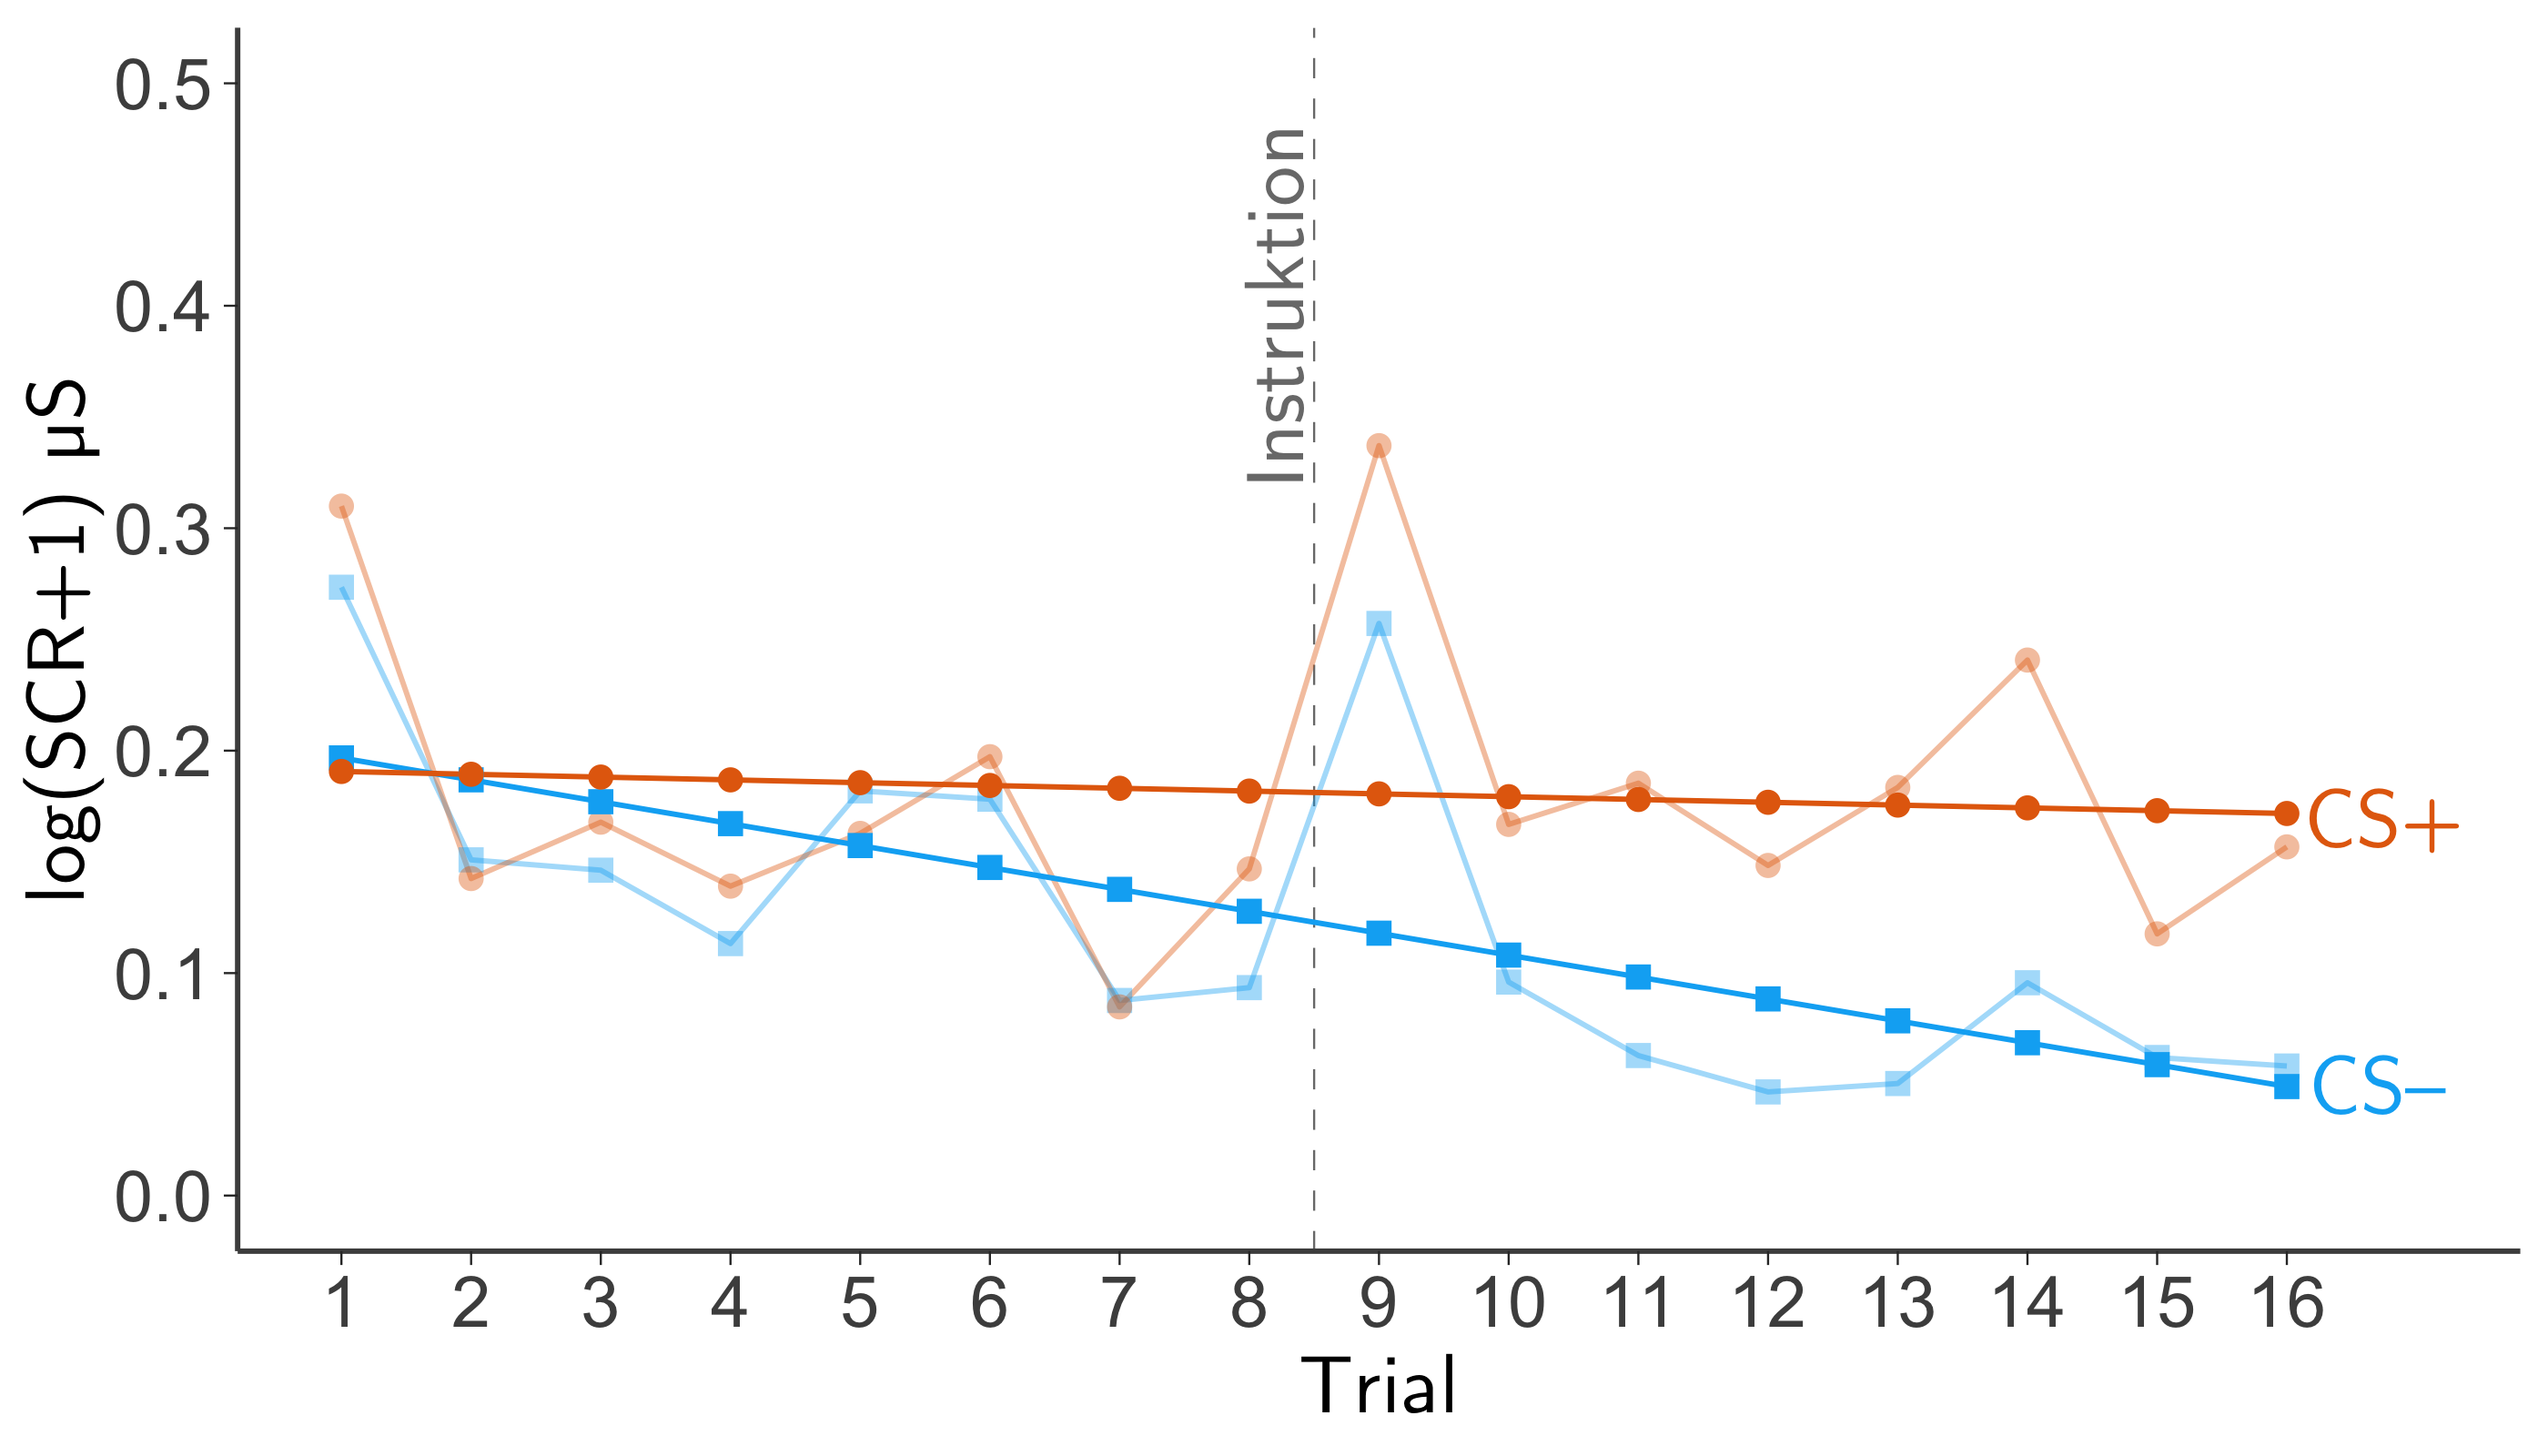
\includegraphics[scale=0.10]{fit_scr.png}};
				\node[inner sep=0pt] (str) at (2,-6.5)
				{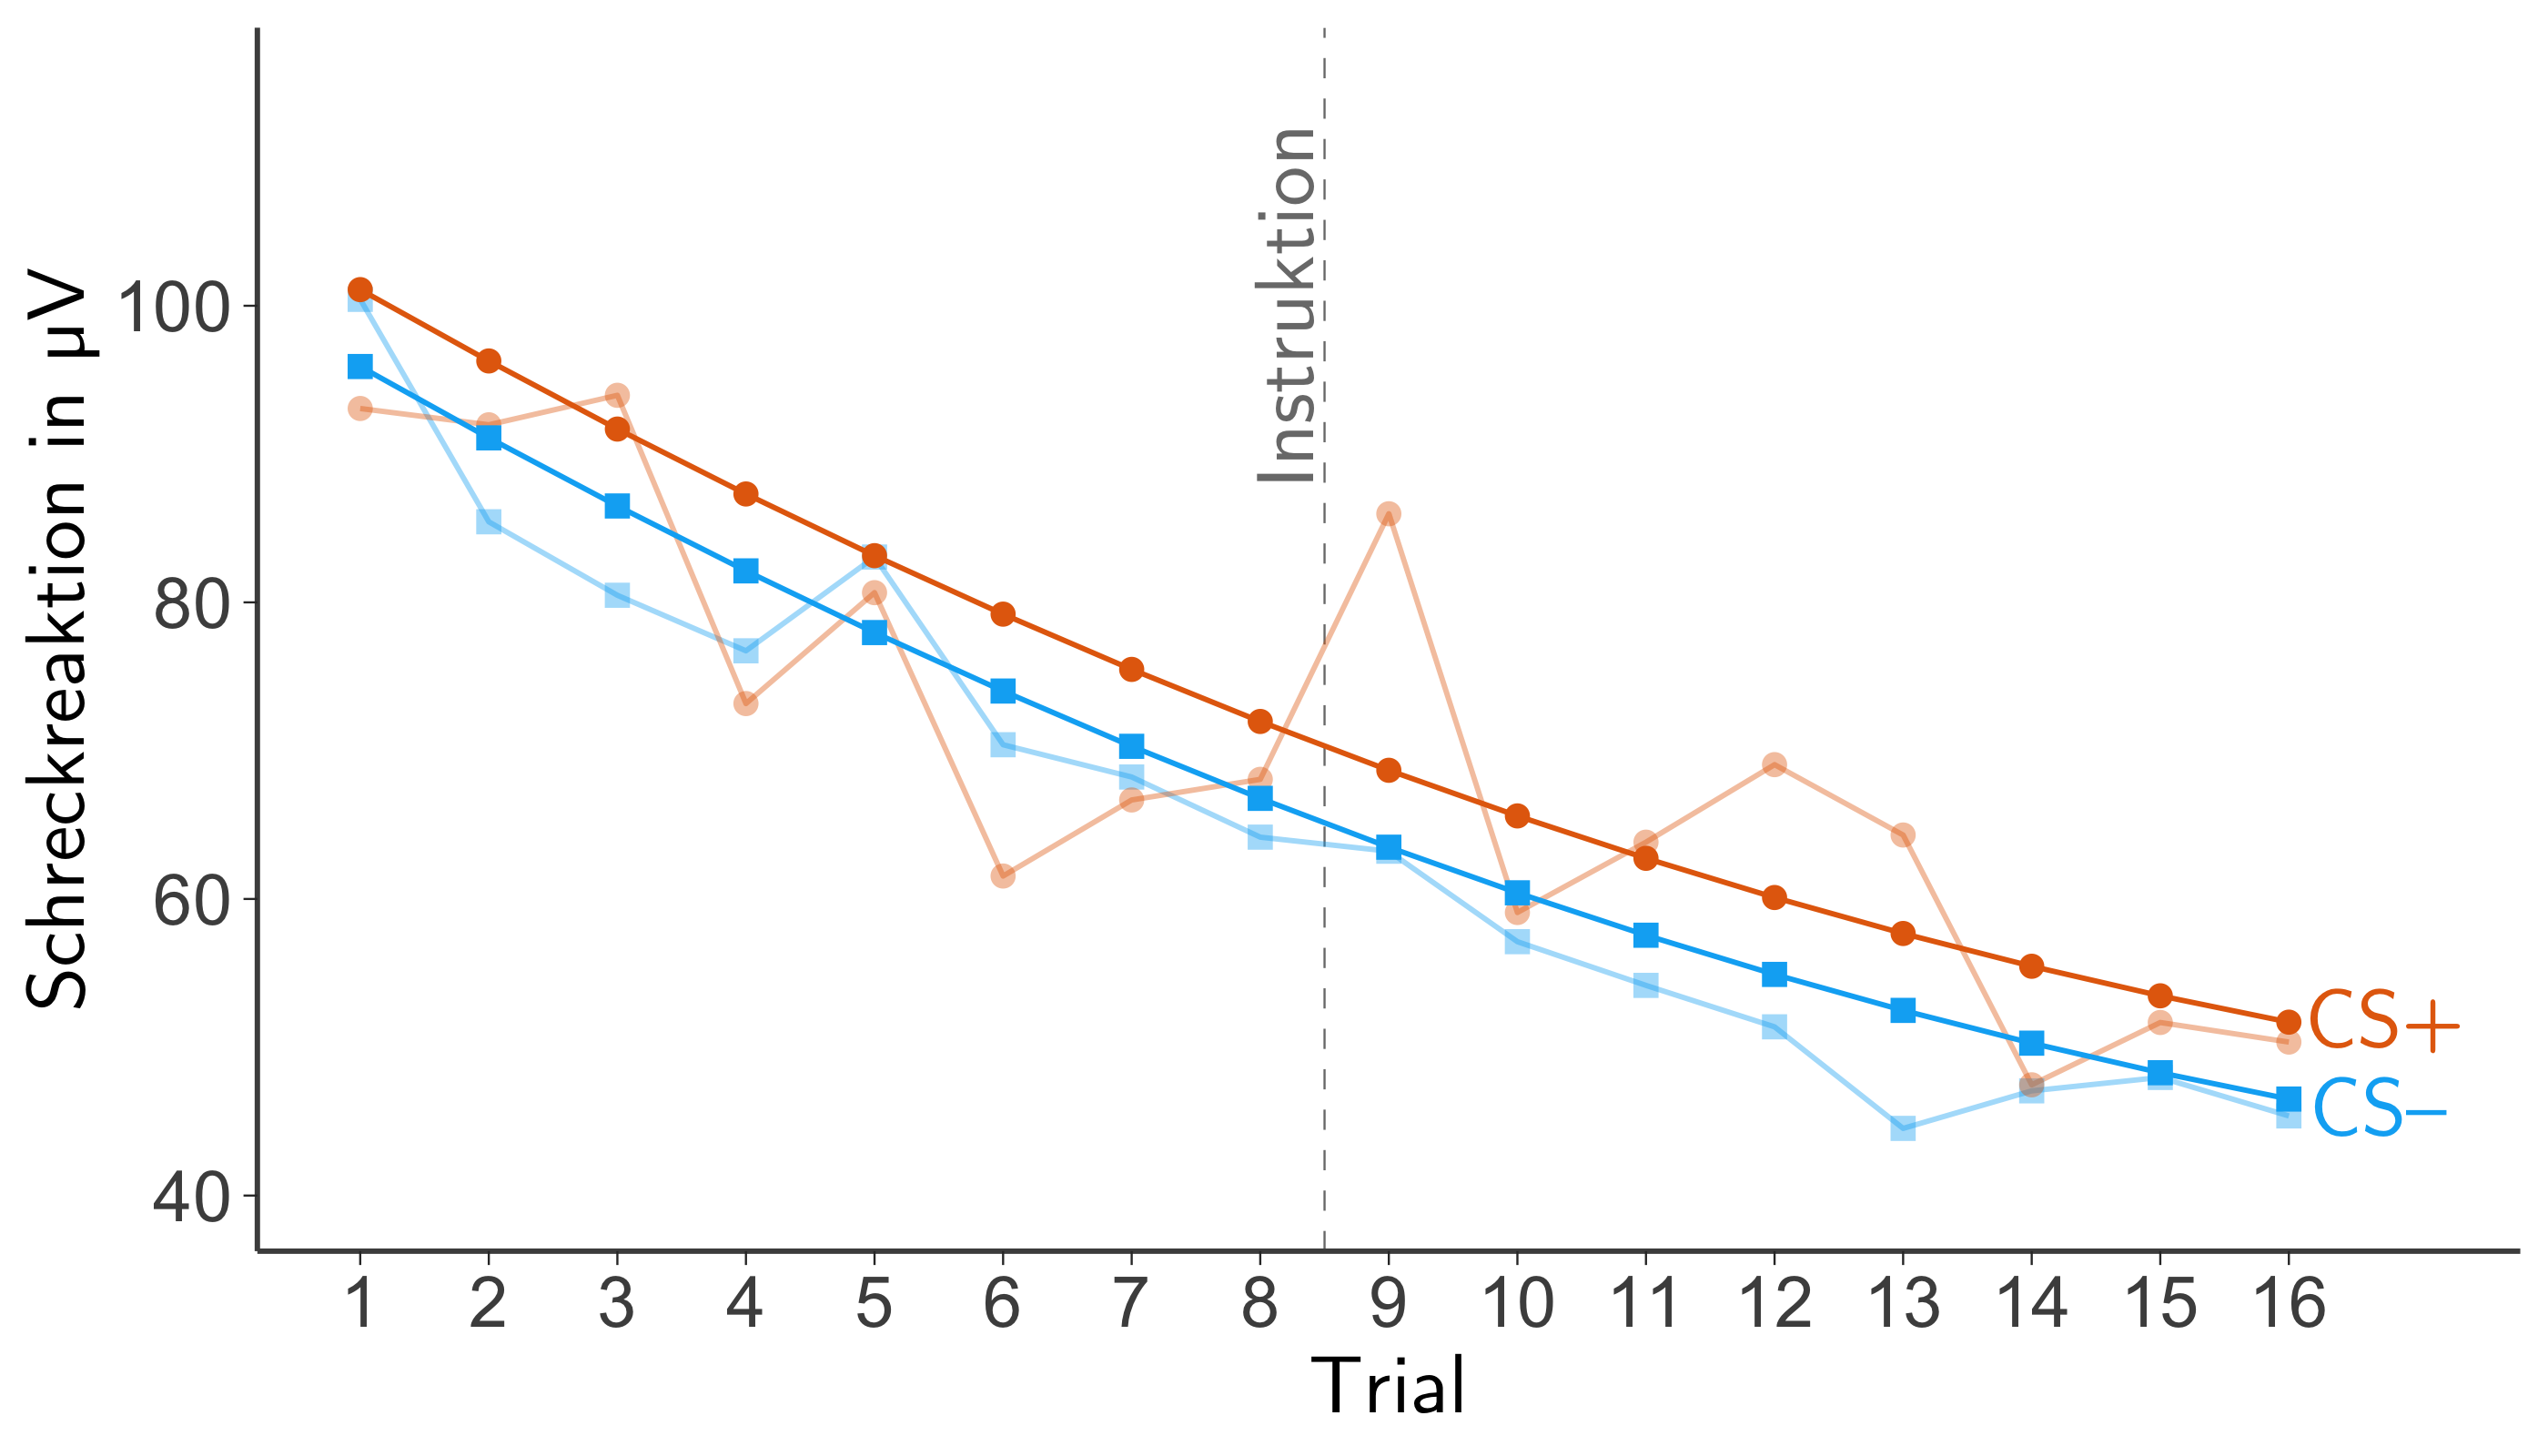
\includegraphics[scale=0.10]{fit_str.png}};
				\node[above left = 0.2cm of scr] (a) {\large{\textsf{\textbf{a}}}};
				\node[above left = 0.2cm of str] (b) {\large{\textsf{\textbf{b}}}};
			\end{tikzpicture}
			\caption[Vorhergesagte Verläufe von Hautleitwert- und Schreckreaktionen]{Vorhergesagte Verläufe von Hautleitwert- (\textsf{\textbf{a}}) und Schreckreaktionen (\textsf{\textbf{b}}) auf Basis des multivariaten Wachstumsmodells, verblasst sind die Rohverläufe.}
			\label{fig:predict}
		\end{figure}
		Im Mittel unterscheidet sich die lineare Änderungsrate für den CS+ also um \SI{0.009}{\micro\siemens} gegenüber der des CS--. Abbildung \ref{fig:predict} zeigt die geschätzten Verläufe nach Stimulustyp getrennt. Hier wird ersichtlich, dass der Unterschied durch einen allmählichen Abfall der Reaktionen auf den CS-- bei relativ gleichbleibender CS+ Reaktion zustande kommt.
		Der beschriebene Interaktionseffekt variiert ebenfalls zwischen Versuchspersonen ($SD=0.006$).
		Die Abweichung der Interaktionsschätzungen für die Versuchspersonen vom festen Effekt $\upbeta_{40}{}^{(1)}$ in Abbildung \ref{fig:randomeffects}e (zentriert bei null) zeigen keine eindeutige Tendenz in Relation zu den zufälligen Intercepts.
		Wenn auch nicht signifikant, deutet allerdings die geschätzte Korrelation zwischen Intercept und Interaktion ($r=-.35$) darauf hin, dass ein höherer Intercept tendenziell mit einem kleineren Unterschied in dem linearen Anstieg zwischen CS+ und CS-- einhergeht.
		
		\begin{table}[hbt] \small \setstretch{1.5} %\doublespacing
			\begin{threeparttable}
				\caption{Ergebnisse des finalen multivariaten Wachstumsmodells}			%ohne Punkt
				\label{tab:final}
				\begin{tabularx}{\textwidth}{lCCCCr}    \toprule
					& \multicolumn{5}{c}{\textbf{Feste Effekte}} \\\cmidrule{2-6} 
					& Beta   & \textit{SE}& \SI{95}{\percent} $KI$		 & $t$   & $p$  \\\hline
					\textbf{SCR} 	 &        &            &                      		       &      &      \\\rowcolor[HTML]{EFEFEF}
					$\quad$Intercept & $0.065$  & $0.029$      &$\left[-0.0008; 0.121\right]$& $2.24$ & $.025$ \\
					$\quad$lin		 & $\hspace*{-0.85em}-0.018$ & $0.004$      &$\left[-0.027; -0.010\right]$& $\hspace*{-0.85em}-4.35$& $<.001$ \\\rowcolor[HTML]{EFEFEF}
					$\quad$CS		 & $0.058$  & $0.012$      &$\left[0.034; 0.083\right]$	 & $4.72$ & $<.001$ \\
					$\quad$CS$\times$lin & $0.009$  & $0.003$      &$\left[0.003; 0.014\right]$	 & $3.00$ & $.003$ \\[+0.5em]	
					\textbf{STR}     &        &            &                      &            &      \\\rowcolor[HTML]{EFEFEF}
					$\quad$Intercept & $\hspace*{-0.5em}59.92$ & $8.49$      &$\left[43.28; 76.57\right]$& $7.06$ & $<.001$ \\
					$\quad$lin		 & $\hspace*{-0.85em}-3.30$ & $0.35$      &$\left[-3.98;-2.60\right]$& $\hspace*{-0.85em}-9.37$& $<.001$ \\\rowcolor[HTML]{EFEFEF}
					$\quad$quad		 & $0.11$  & $0.05$      &$\left[0.01; 0.21\right]$	 & $2.20$ & $.028$ \\
					$\quad$CS 		 & $5.19$  & $1.87$      &$\left[1.53; 8.85\right]$	 & $2.78$ & $.006$ \\
					%&&&&&\\[-0.2em]\bottomrule
				\end{tabularx}
				\begin{tabularx}{\textwidth}{lCccccc}    \toprule
					& \multicolumn{6}{c}{\textbf{Zufällige Effekte}}\\ \cmidrule{2-7} 
					& \multirow[c]{2}{*}{\textit{SD}} & \multirow[c]{2}{*}{\SI{95}{\percent} $KI$} && \multicolumn{3}{c}{Korrelationen\tnote{a}}    \\ 
					&&       && Intercept (SCR) & Intercept (STR)& CS$\times$lin (SCR)      \\ \hline \rowcolor[HTML]{EFEFEF}
					Intercept (SCR) 		 & $0.130$ &$\left[0.10;0.17\right]$&& --           	  &      		 &      	\\
					Intercept (STR) 		 & $\hspace*{-0.5em}49.98$&$\left[39.8;62.7\right]$&& $.14$	          & --     		 &       \\\rowcolor[HTML]{EFEFEF}
					CS$\times$lin (SCR) 	 & $0.006$ &$\left[0.004;0.009 \right]$&& $\hspace*{-0.85em}-.35$          & $-.04$ 		 & --    \\
					CS$\times$lin (STR) 	 & $1.341$ &$\left[0.99;1.81\right]$&& $\hspace*{-0.85em}-.05$          & $\hspace*{0.55em}-.48^*$ 		 & $-.29$ \\[-0.2em]
					\bottomrule
				\end{tabularx}
				\begin{tablenotes}[normal, flushleft, para]
					\footnotesize{
						\item \textit{Anmerkungen.} Konfidenzintervalle, Signifikanz und $p$-Werte berechnet über Normalapproximationen der Verteilung der geschätzten Effekte. Die daraus angenäherte $t$-Teststatistik hat $df=2374$ Nenner-Freiheitsgrade.
						\item[a] bei ${}^{*}$ signifikant auf \SI{5}{\percent} Niveau.}
				\end{tablenotes}
			\end{threeparttable}
		\end{table}	
		
		Für die Schreckreaktion beschreibt der geschätzte Intercept mit \SI{59.92}{\micro\volt} ebenfalls die mittlere Reaktion zwischen dem $8.$ und $9.$ CS-- Trial ($SE=8.49$). Als zufällig modelliert variiert dieser Intercept mit einer geschätzten Standardabweichung von $49.98$ zwischen Versuchspersonen. Abbildungen \ref{fig:randomeffects}b und \ref{fig:randomeffects}d zeigen die Versuchspersonen-Intercepts als Abweichungen vom mittleren Intercept. Hier liegen die geschätzten Intercept nur für zwei knapp unter Null.
		Der Koeffizient $\upbeta_{10}{}{(2)}$ mit der Schätzung $-3.3$ ($SE=0.35$) reflektiert nun die momentane Änderungsrate der Schreckreaktion für den CS-- in der Mitte des Akquisitionstrainings. Die quadratische Änderungsrate für den CS-- ist positiv ($\upbeta_{20}{}{(2)}=0.11$, $SE=0.05$). Daraus und in Verbindung mit Abbildung \ref{fig:predict} wird deutlich, dass die Wachstumskurven für die Schreckreaktion als nach oben geöffnete, gestauchte Parabeln modelliert werden. 
		Auch hier hat der Stimulustyp einen substanziellen Einfluss. Im Mittel sind die Schreckreaktionen der Versuchspersonen auf den CS+ \SI{5.19}{\micro\volt} höher als auf den CS-- ($SE=1.87$). Allerdings ist die Interaktion -- sprich der Unterschied zwischen CS+ und CS-- in der linearen Änderungsrate -- im Gegensatz zur SCR statistisch nicht bedeutsam. Über die Zeit hinweg wird der Unterschied zwischen CS+ und CS-- daher als konstant modelliert (Abb. \ref{fig:predict}).
		Die Varianz, die Versuchspersonen in dieser Interaktion aufzeigen, ist wiederum Teil des Modells. Für den zufälligen Effekt zeigt sich, dass die Interaktionseffekte zwischen Versuchspersonen mit einer Standardabweichung von $1.34$ variieren.
		In der Abbildung \ref{fig:randomeffects}f lässt sich durch Hinzunahme der nach Größe geordneten Interceptschätzungen aus \ref{fig:randomeffects}d ein Abwärtstrend vermuten, den die geschätzte Korrelation von $r=-.48$ zwischen Intercept und Interaktion bestätigt. Für Versuchspersonen mit höherer Reaktion auf den CS-- in der Mitte des Trainings werden eher kleinere Unterschiede im linearen Anstieg zwischen CS+ und CS-- vorhergesagt. Der \nameref{appE} enthält unterstützend paarweise Streudiagramme zwischen den geschätzten zufälligen Effekten innerhalb und zwischen den beiden Reaktionsmaßen.
		In der multivariaten Betrachtung zeigt sich ein positiver, kleiner und nicht signifikanter Zusammenhang ($r=.14$). %Ein größerer Mittelwert in der Hautleitwertreaktion auf den CS-- in der Mitte des Trainings geht daher3 tendenziell mit einem größeren Mittelwert der Schreckreaktion einher. 
		Bei den beiden Interaktionseffekten \textit{CS$\times$lin} schätzt das Modell eine negative Korrelation von $r=-.29$ zwischen den abhängigen Variablen, die allerdings wiederum nicht signifikant ist. Tendenziell geht damit ein größerer Interaktionsterm auf dem einen Reaktionsmaß mit einer kleineren Interaktion auf dem anderen Maß einher.
		%Die vorhergesagte mittlere Reaktion auf einen CS+ in der Mitte des Akquisitionstrainings wäre damit $58.12+5.26=63.38$
	
		\begin{figure}[ht]
			\centering
			\begin{tikzpicture}[remember picture] \centering		
				\node[inner sep=0pt] (a1) at (0,0)
				{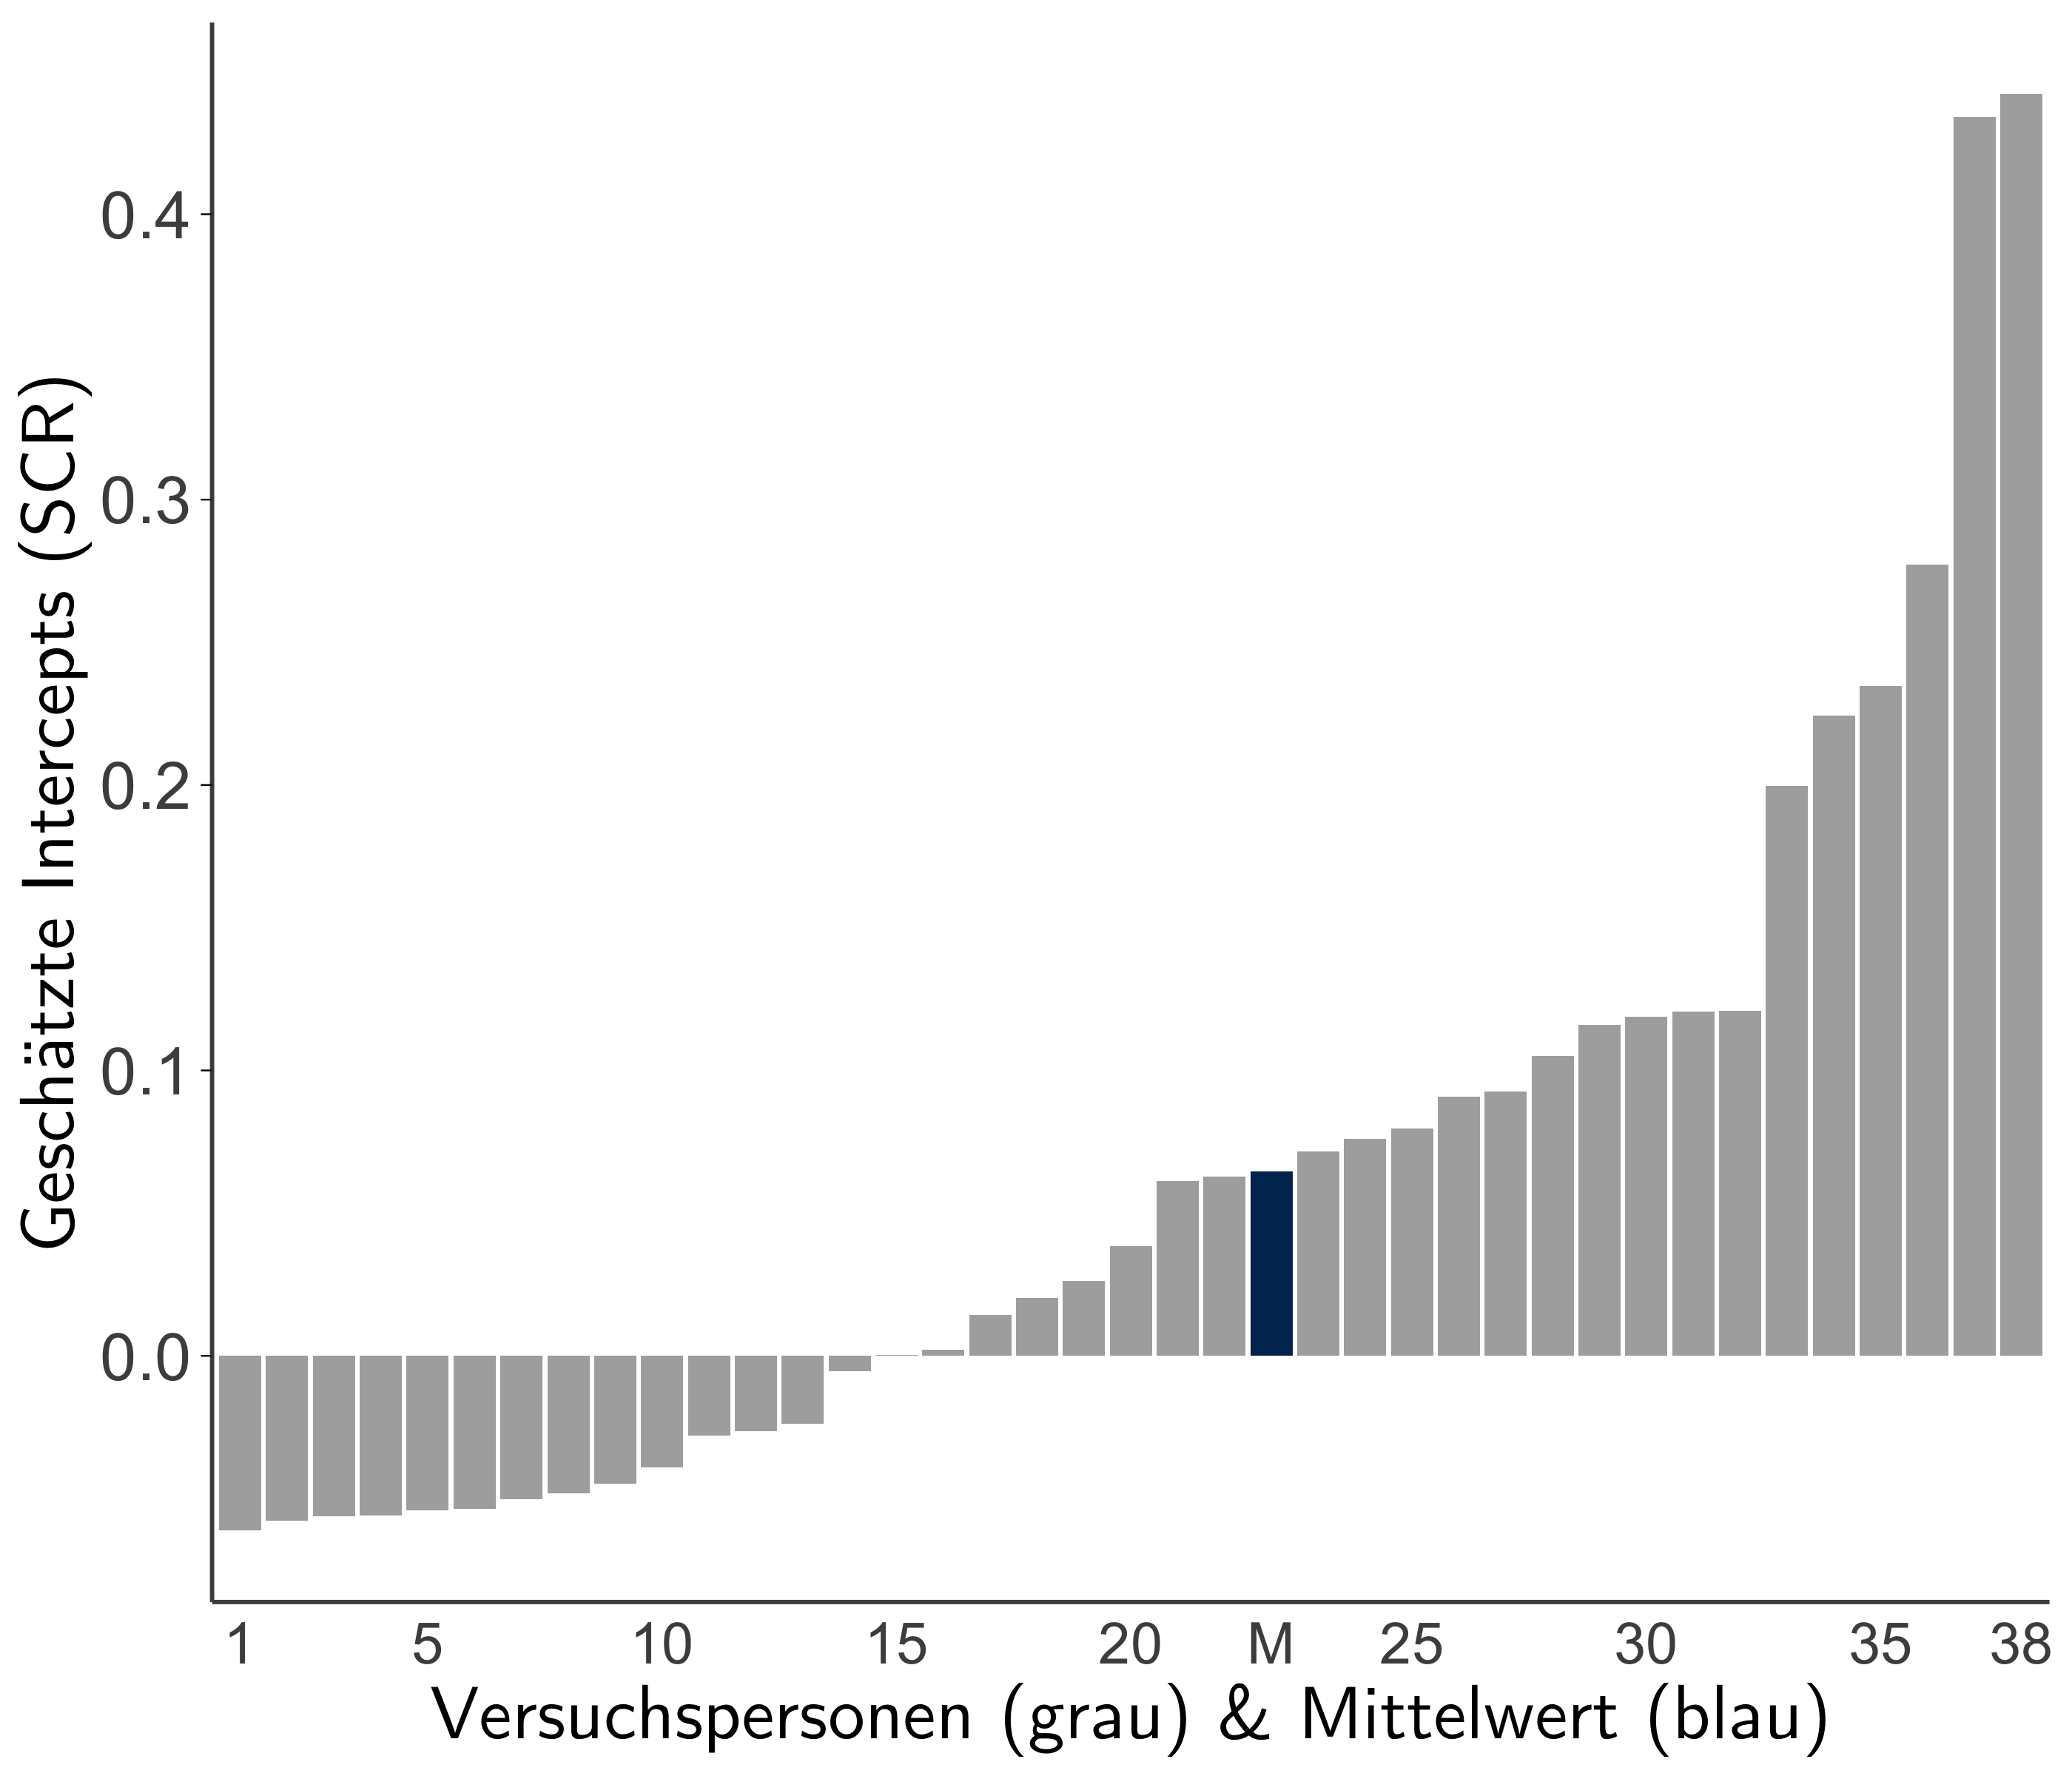
\includegraphics[scale=0.068]{r1.png}};
				\node[inner sep=0pt, below = 0.7cm of a1] (a2)
				{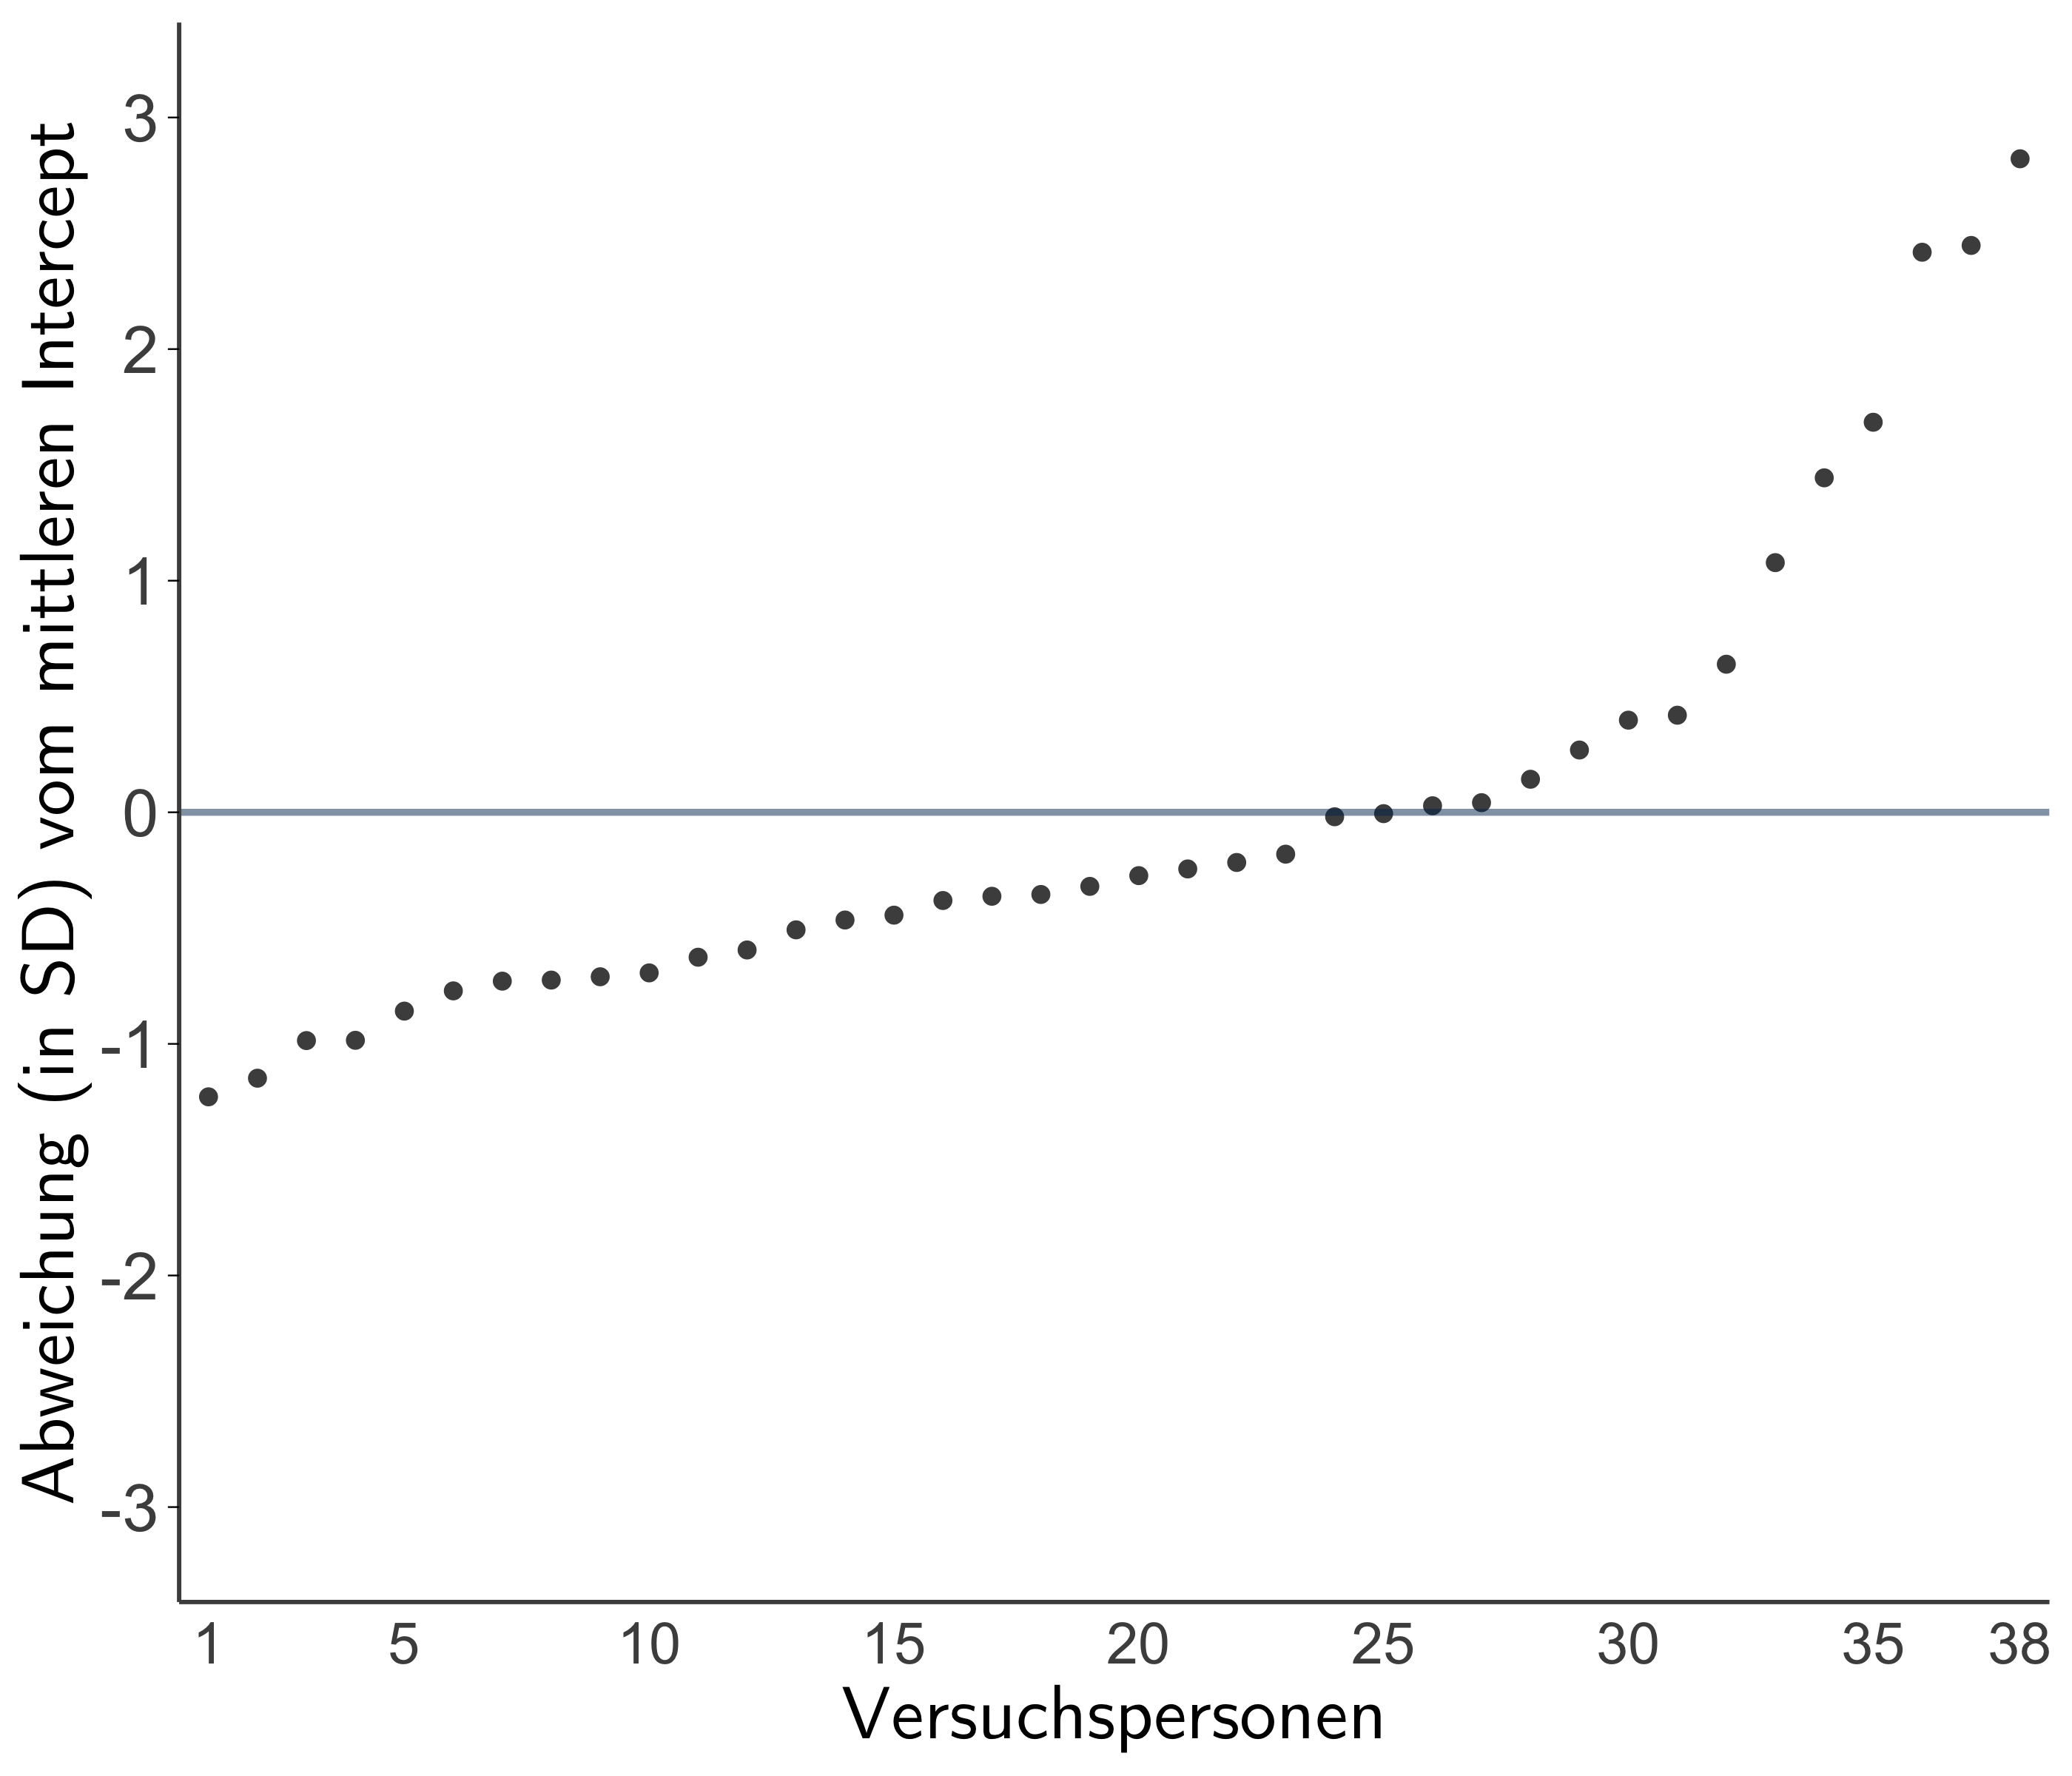
\includegraphics[scale=0.068]{r4.png}};
				\node[inner sep=0pt, right = 1cm of a1] (a3)
				{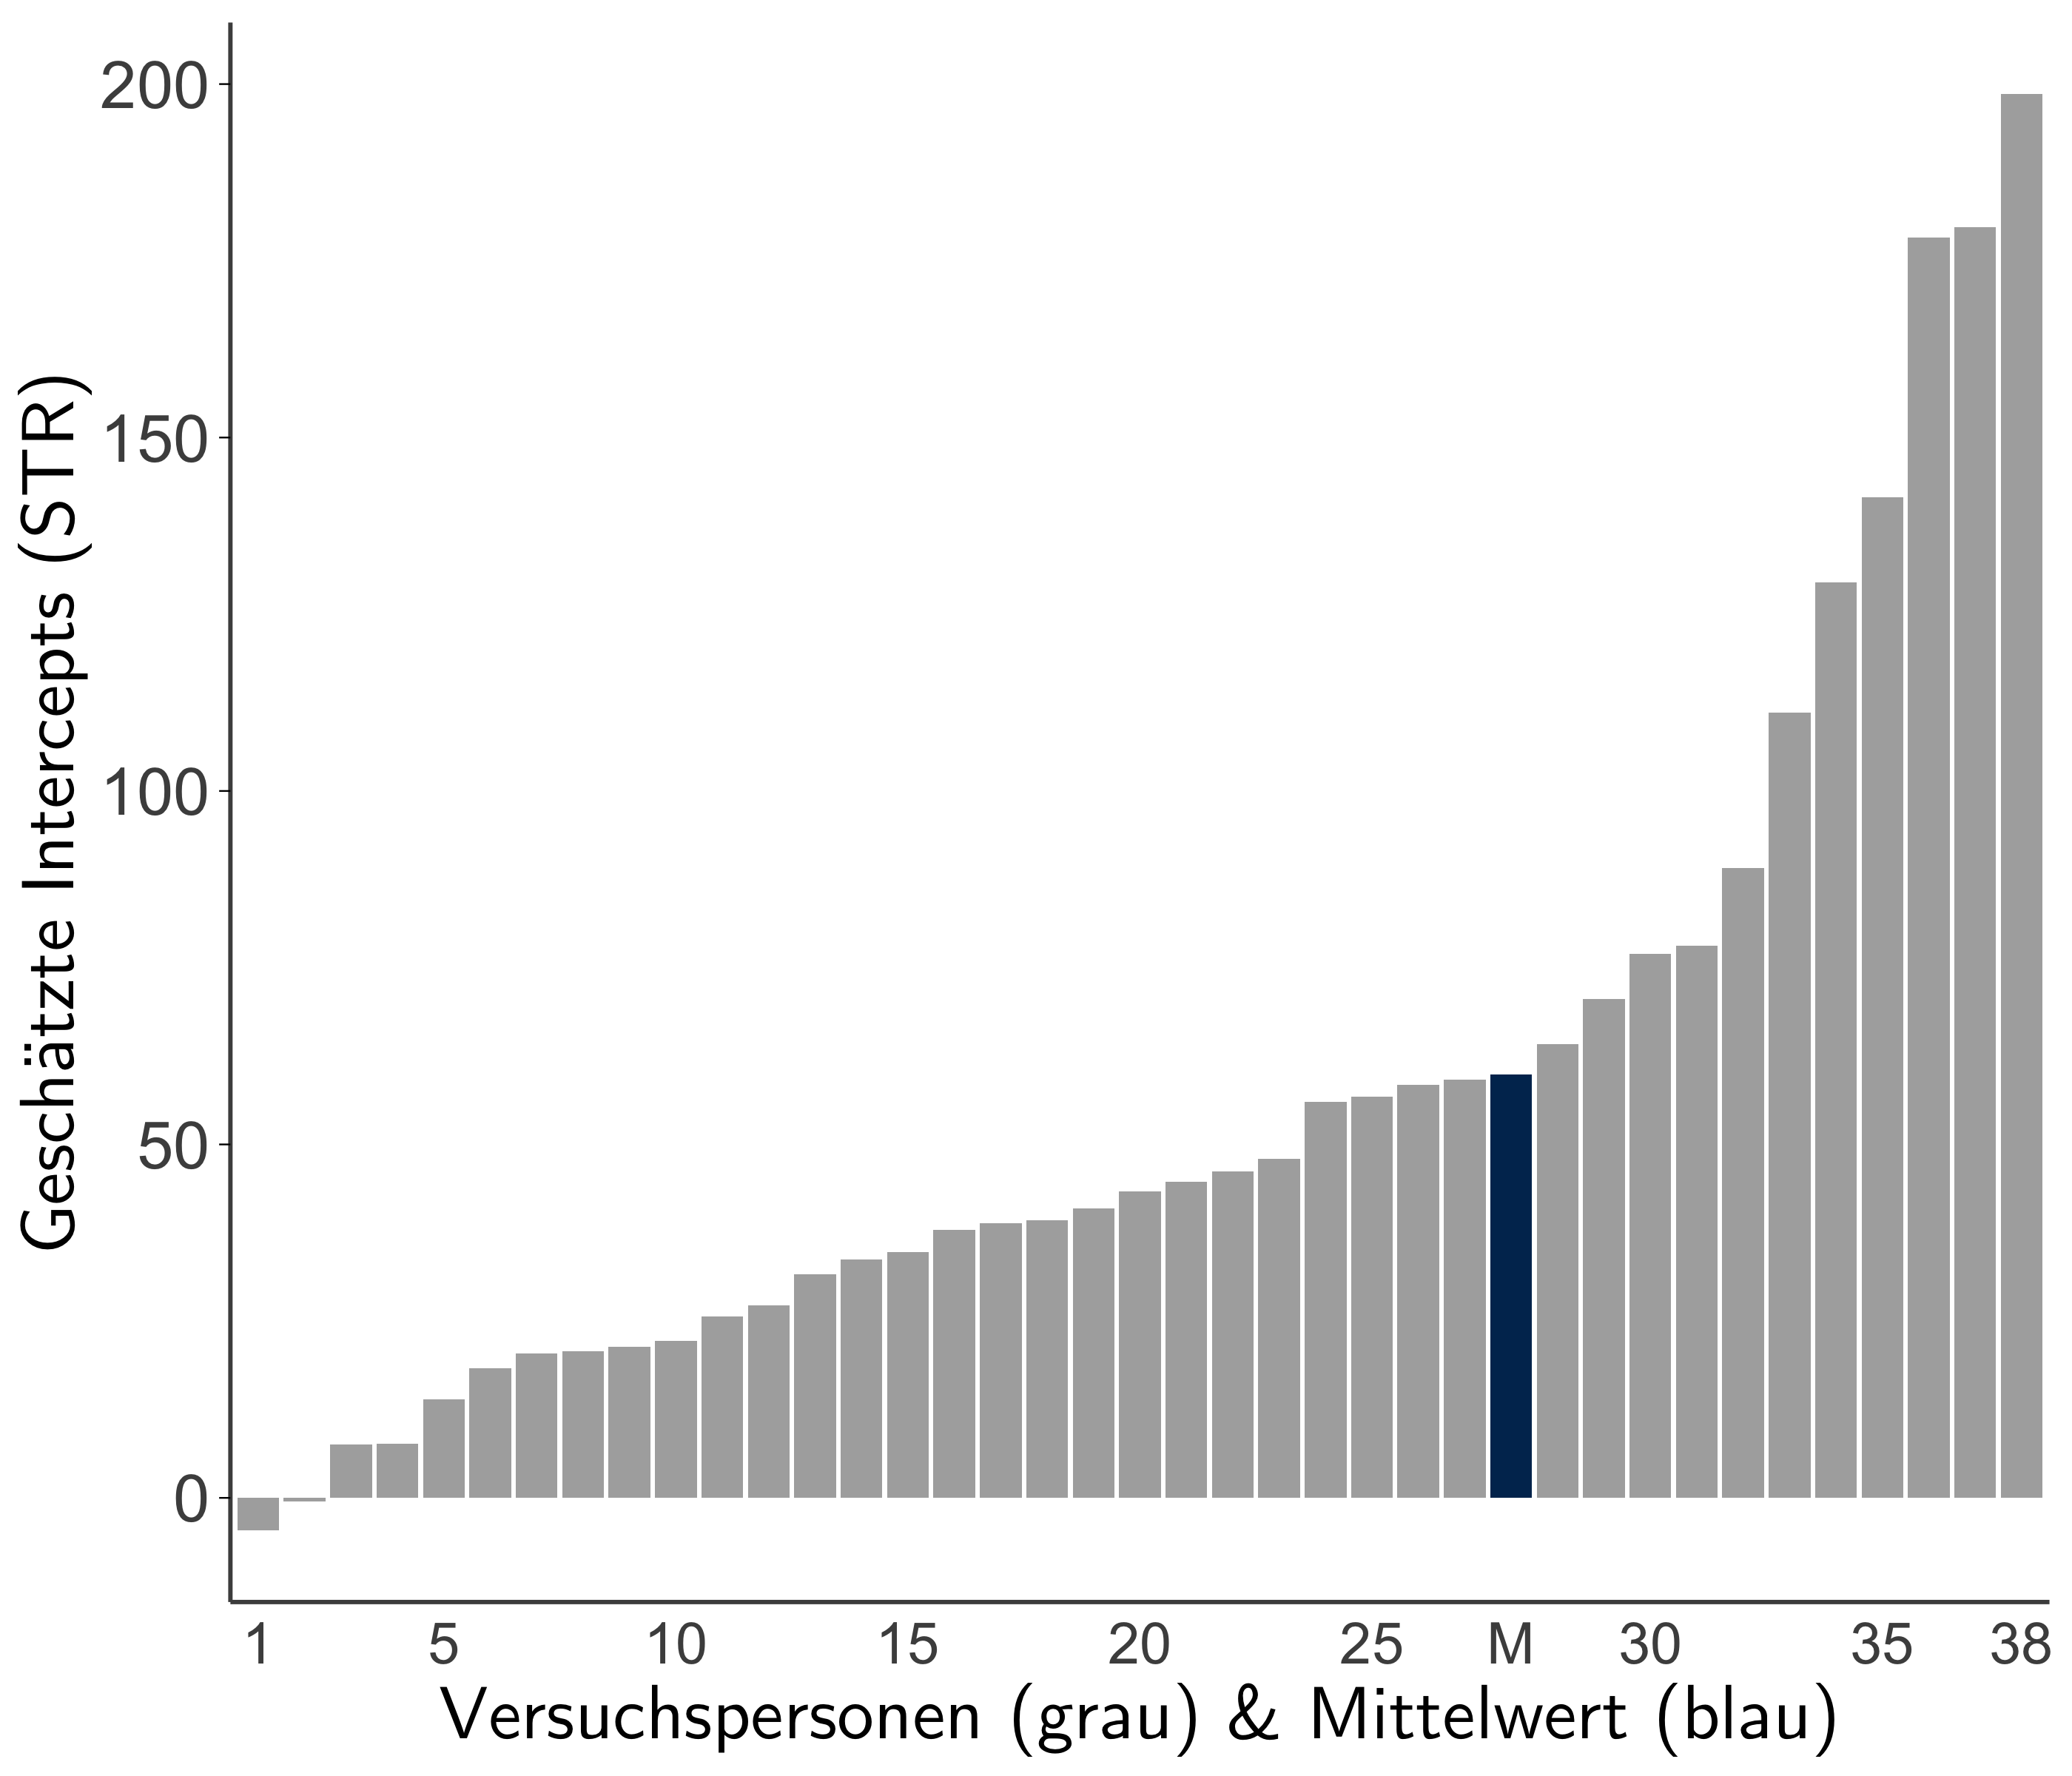
\includegraphics[scale=0.068]{r2.png}};
				\node[inner sep=0pt, below = 0.7cm of a3] (a4)
				{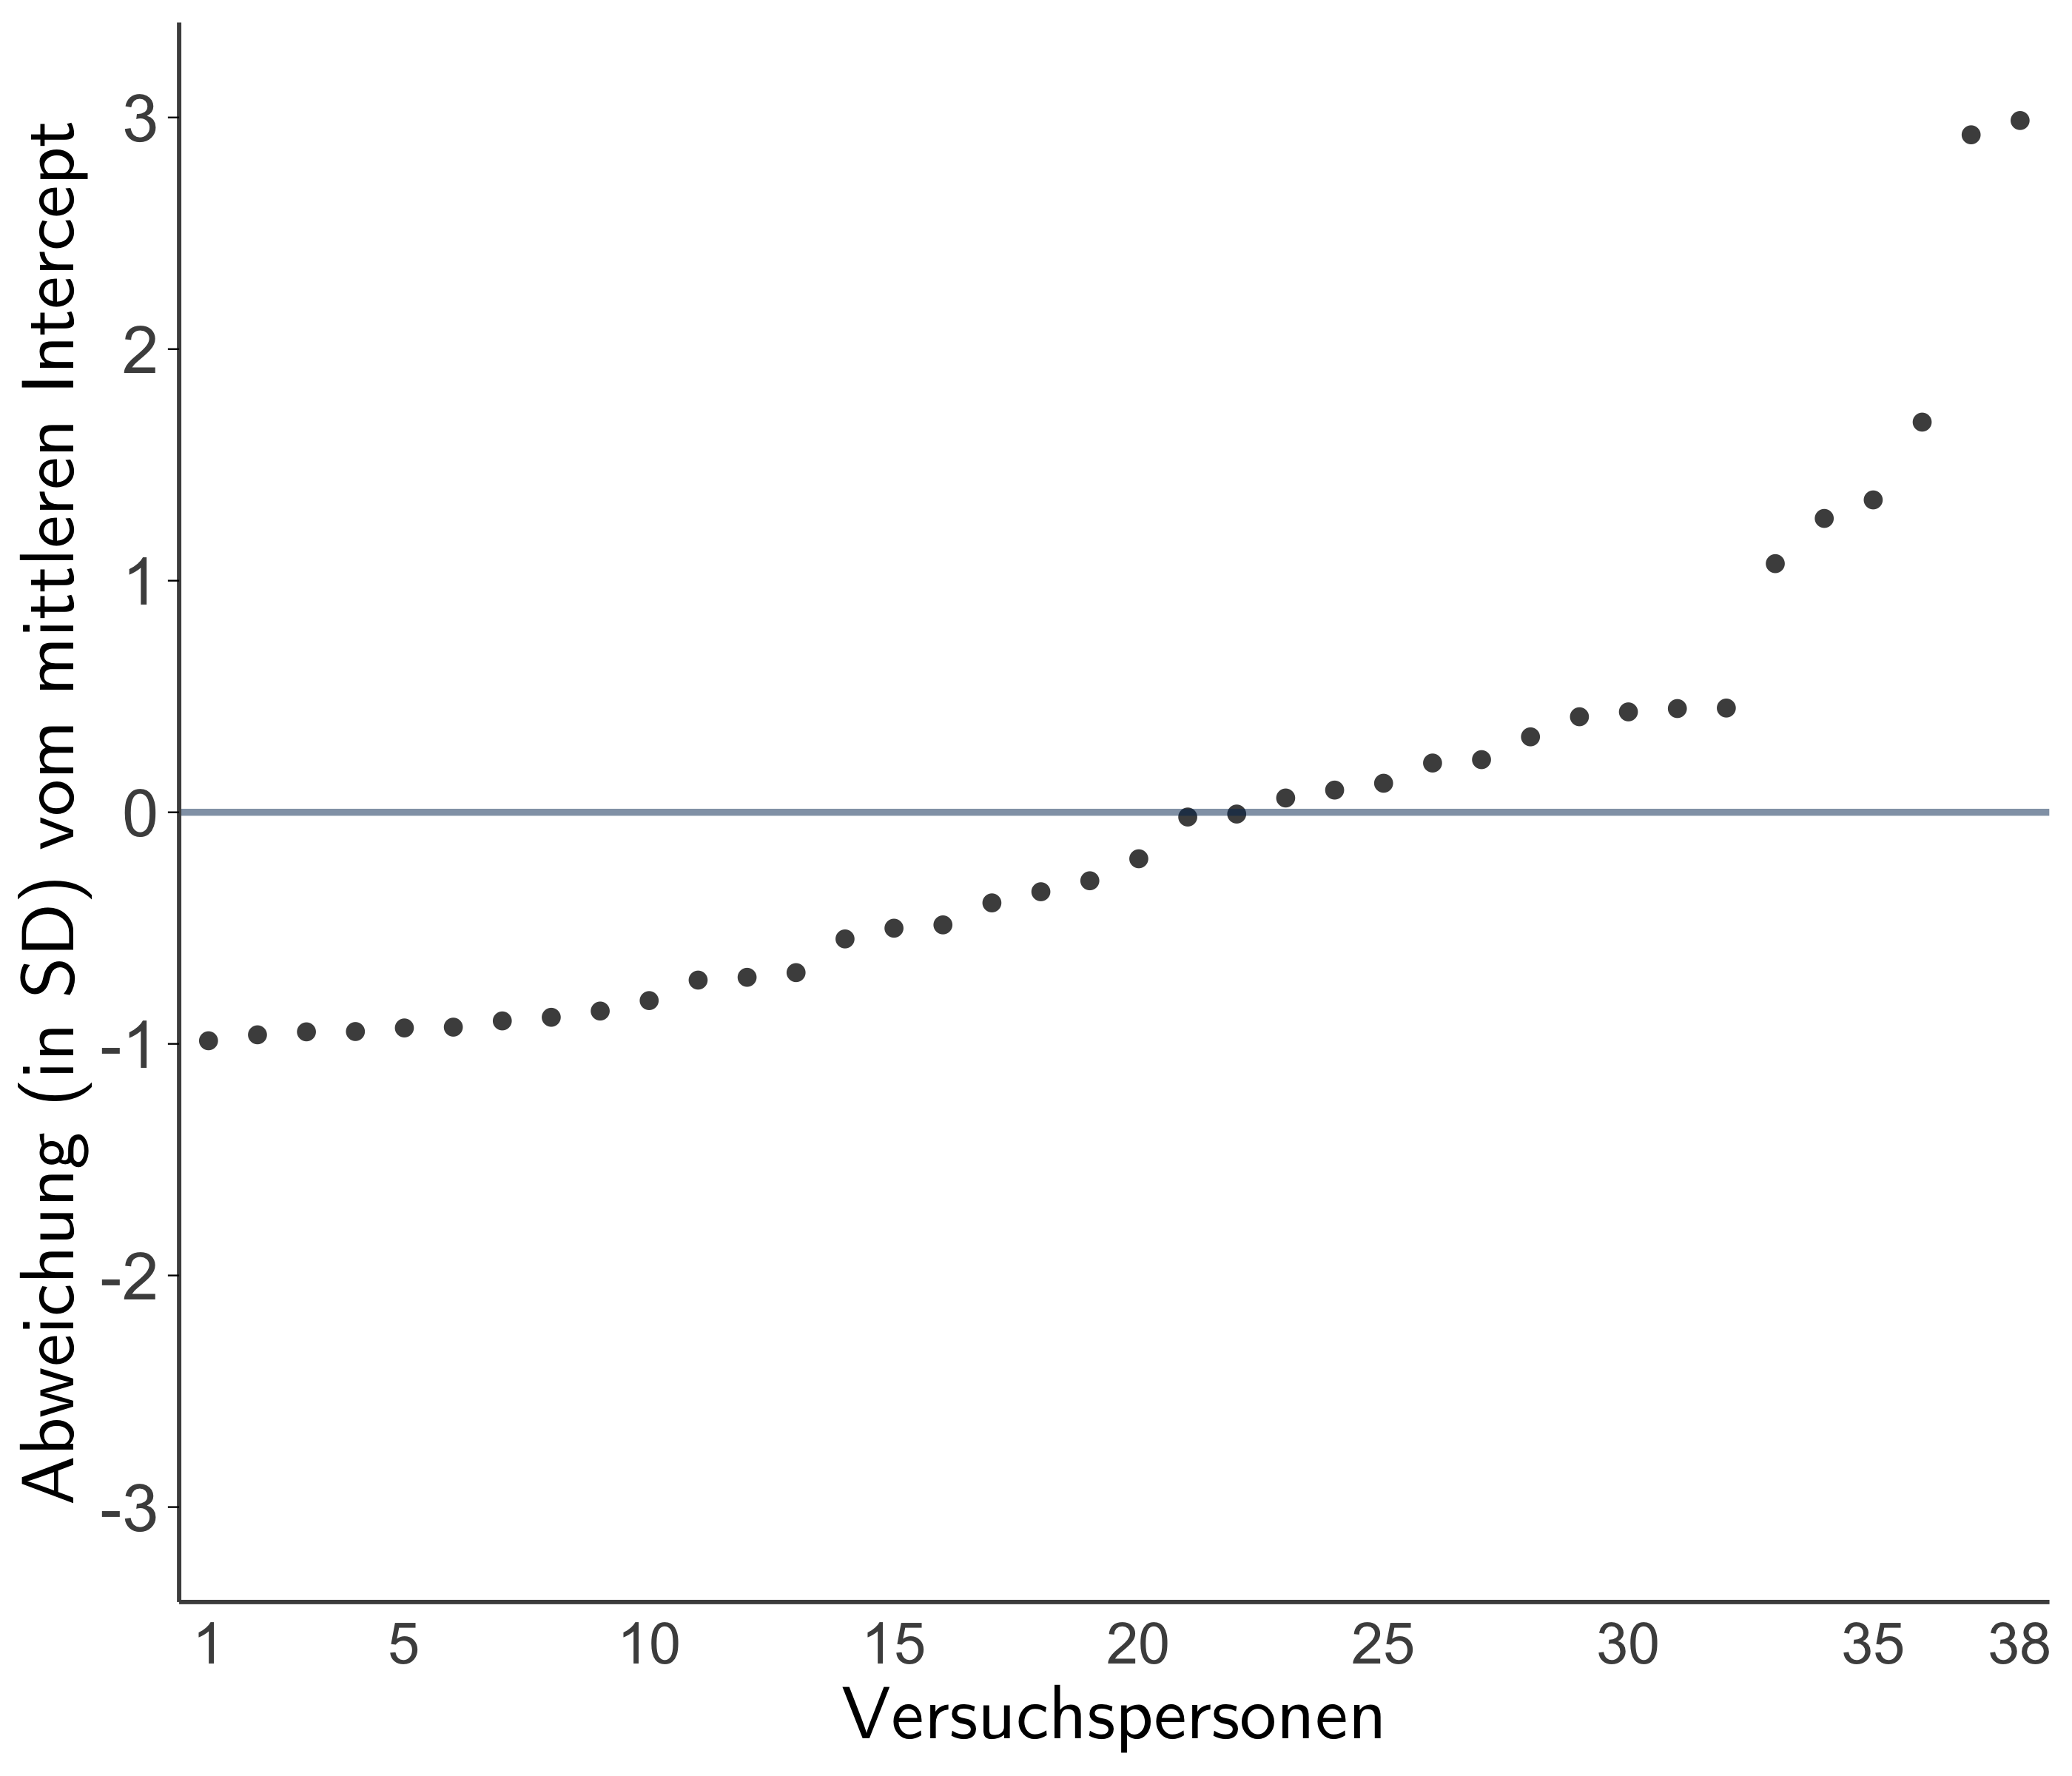
\includegraphics[scale=0.068]{r5.png}};
				\node[inner sep=0pt, below = 0.7cm of a2] (a5)
				{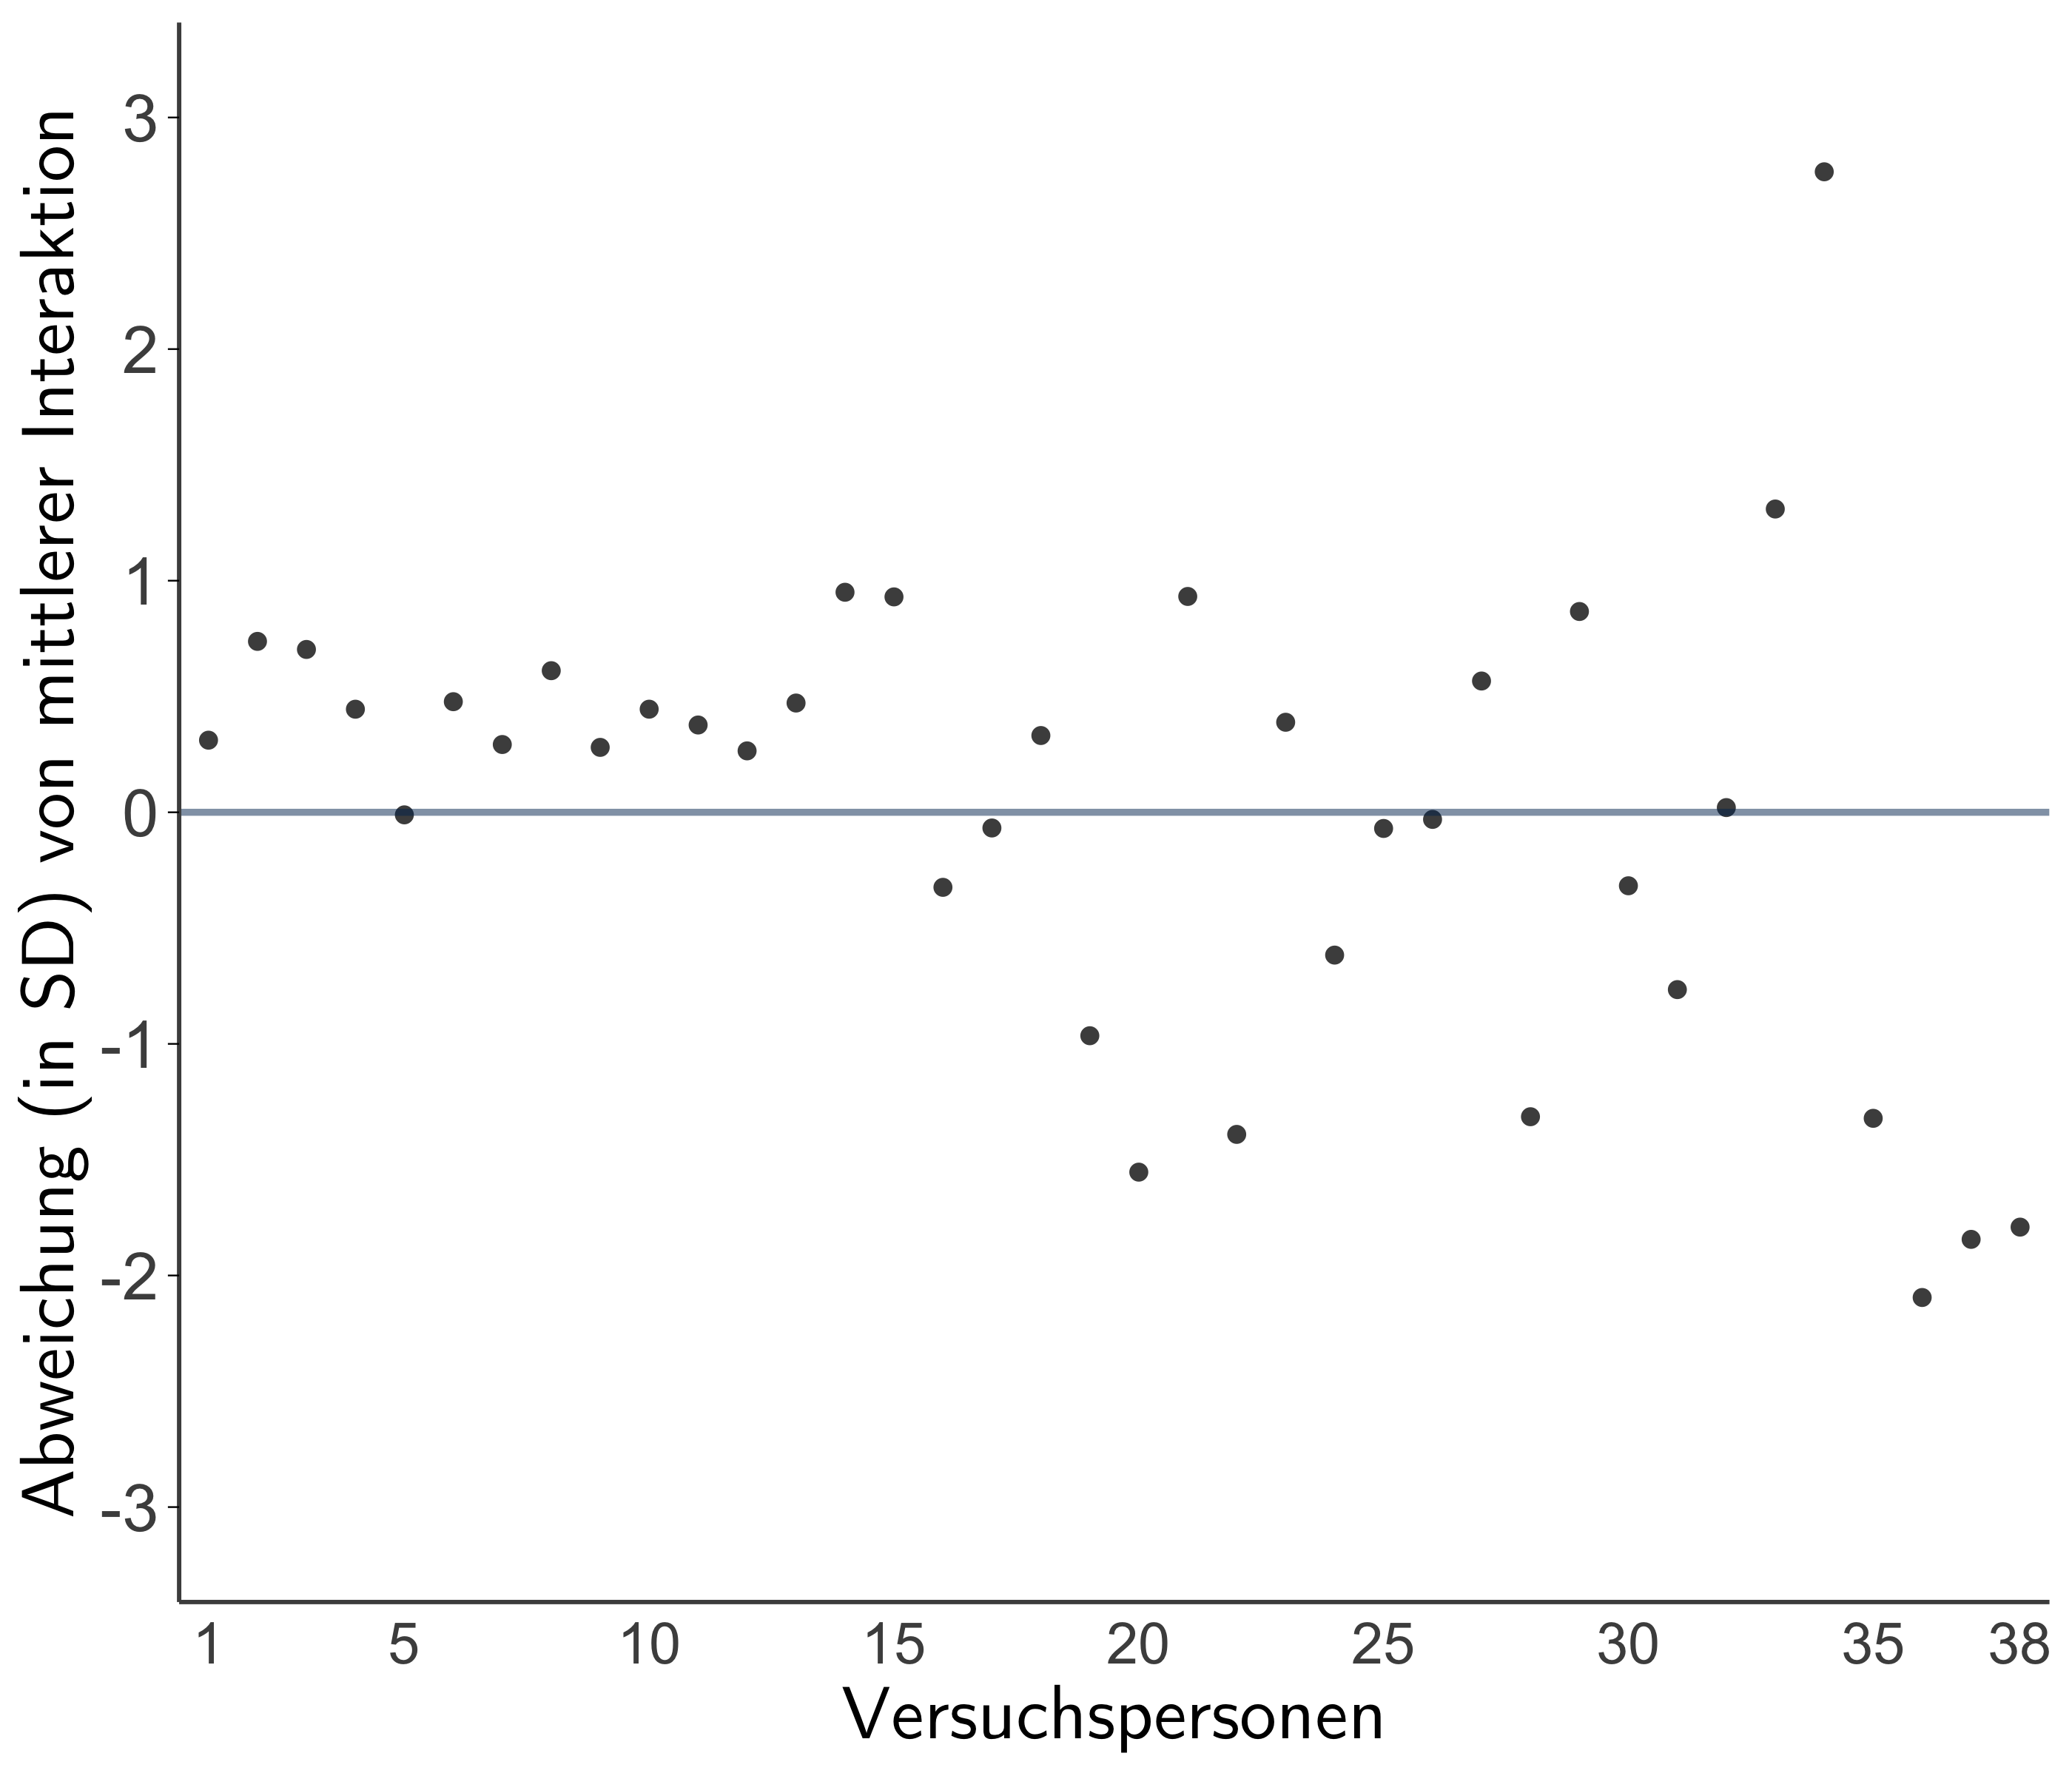
\includegraphics[scale=0.068]{r7.png}};
				\node[inner sep=0pt, right = 1cm of a5] (a6)
				{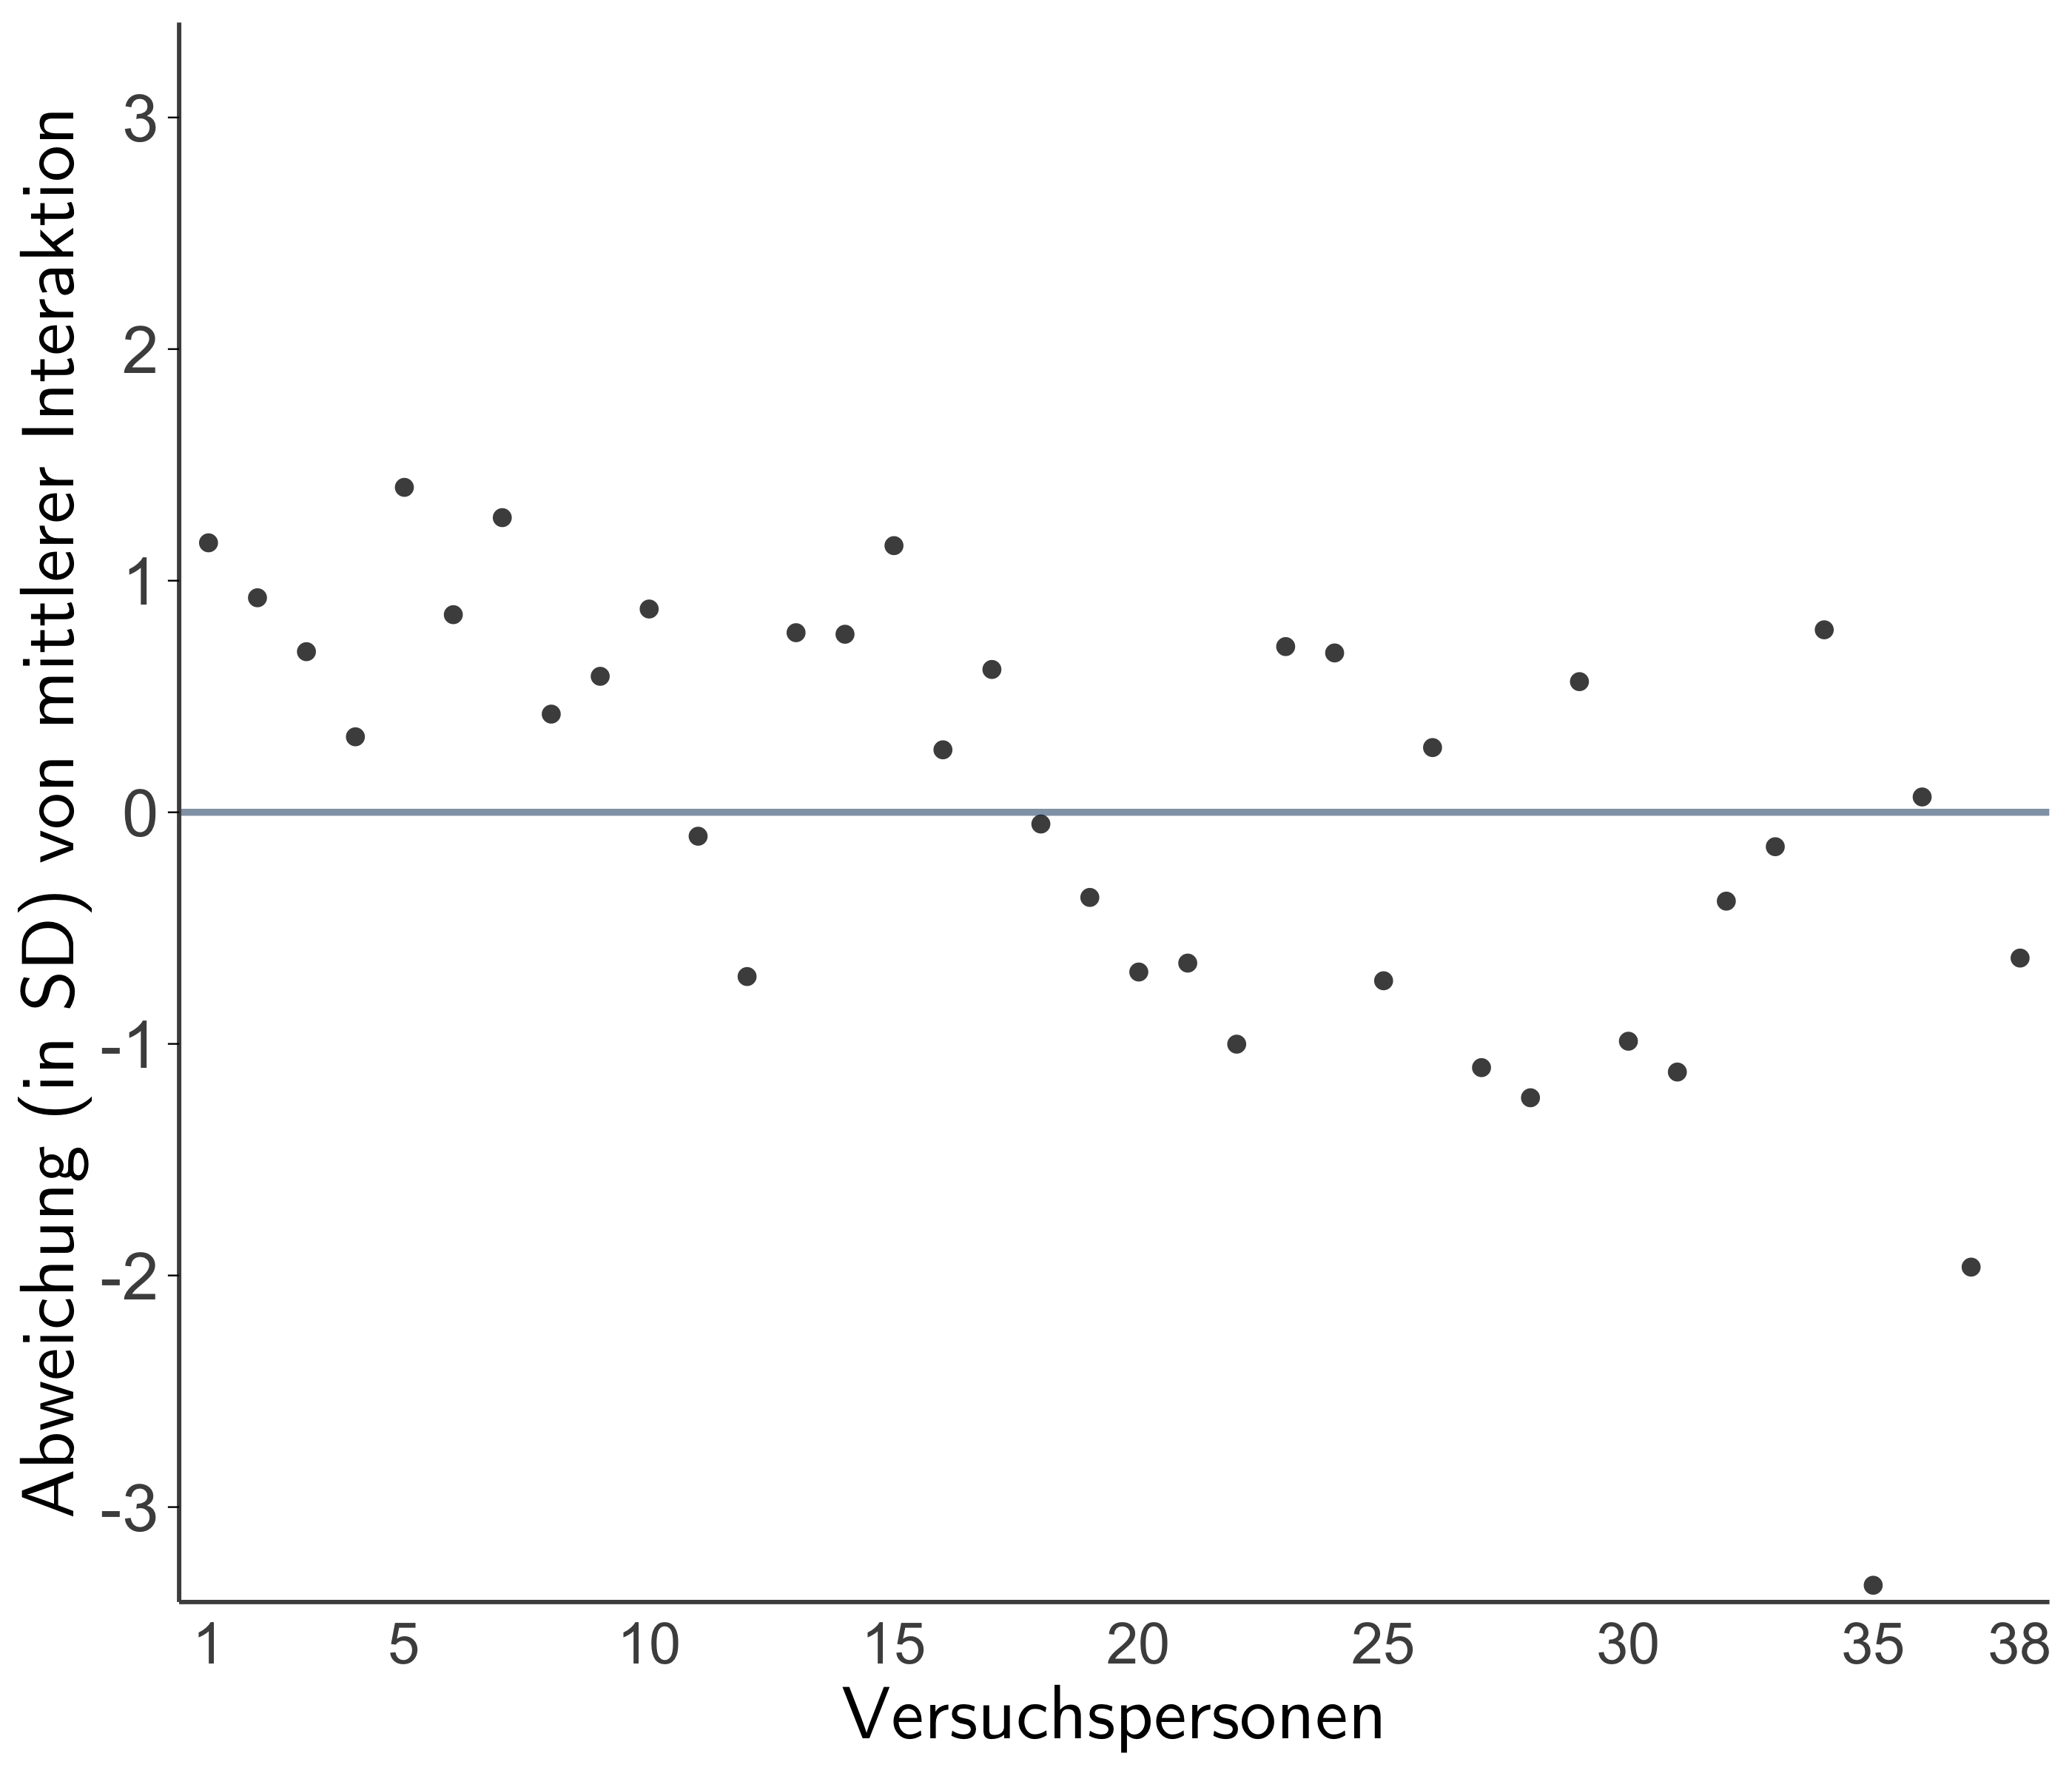
\includegraphics[scale=0.068]{r6.png}};
				\node[above = 0.7cm of a1] (SCR) {\large{\textsf{\textbf{SCR}}}};
				\node[above = 0.7cm of a3] (STR) {\large{\textsf{\textbf{STR}}}};
				\node[above left = 0.1cm and -0.5cm of a1] (a) {\large{\textsf{\textbf{a}}}};
				\node[above left = 0.1cm and -0.5cm of a3] (b) {\large{\textsf{\textbf{b}}}};
				\node[above left = 0.1cm and -0.5cm of a2] (c) {\large{\textsf{\textbf{c}}}};
				\node[above left = 0.1cm and -0.5cm of a4] (d) {\large{\textsf{\textbf{d}}}};
				\node[above left = 0.1cm and -0.5cm of a5] (e) {\large{\textsf{\textbf{e}}}};
				\node[above left = 0.1cm and -0.5cm of a6] (f) {\large{\textsf{\textbf{f}}}};
			\end{tikzpicture}
			\caption[Abbildung der zufälligen Intercepts \& Interaktionen]
			{(\textbf{a}) und (\textbf{b}): Versuchspersonen-Intercepts des Modells mit dem mittleren (globalen) Intercept in blau. (\textbf{c}) und (\textbf{d}): Abweichungen dieser Intercepts vom mittleren Intercept (zentriert bei null) skaliert in Standardabweichungen. (\textbf{e}) und (\textbf{f}): Abweichungen der Interaktionsschätzungen für die einzelnen Versuchspersonen (skaliert in $SD$). Abbildungen motiviert durch \textcite{METEYARD2020}.}
			\label{fig:randomeffects}
		\end{figure} 

%%%%%%%%%%%%%%%%%%%%%%%%%%%%%%%%%%%%%%%%%%%%%
%%%%%%%%%%%%ANNAHMEN PRÜFEN%%%%%%%%%%%%%%%%%%
%%%%%%%%%%%%%%%%%%%%%%%%%%%%%%%%%%%%%%%%%%%%%

	\section{Prüfen der Modellannahmen}		\label{assumptions}

		Alle Abbildungen für die Prüfung der Modellannahmen sind in \nameref{appF} enthalten. 
	%RESID VS. FITTED
		Das Streudiagramm zwischen Residuen und angepassten Werten für die höchste Gruppierungsebene zeigt für die SCR einen klaren Bodeneffekt bei kleinen angepassten Werten. Dies scheint eine wesentliche Einschränkung des Modells zu sein, die durch die verhältnismäßig hohe Anzahl an Nullreaktionen und Reaktionen nahe null zustande kommt. Residuen sind bei diesen Reaktionen zwangsläufig positiv, sodass hier eine Varianzeinschränkung vorliegt.
		Für die Schreckreaktionen ist diese Verletzung der Varianzhomogenität gering ausgeprägt. Tendenziell ist die Residuenvarianz für kleine angepasste Werte ($\leq 50$) etwas geringer, für die Werte ab $50$ lässt sich jedoch eine zufällige gleichmäßige Streuung beobachten.
	%QQPLOT HISTOGRAMM
		Für die Normalverteilungsannahme der Residuen auf Ebene der Versuchsperson wird eine visuelle Analyse der Häufigkeitsverteilung durch Histogramme und Q-Q-Diagramme für beide  abhängigen Variablen durchgeführt.
		Sowohl die Histogramme als auch die Q-Q-Diagramme zeigen eine substanzielle Abweichung von der Normalverteilung für die Residuen. Für die Hautleitwertreaktionen ist diese stärker als für die Schreckreaktion. 
		Die Häufigkeitsverteilungen deuten daraufhin, dass die Residuen für beide Reaktionsmaße zum Teil starke Ausreißer aufweisen. Außerdem scheint die ausgeprägte Spitze der Verteilung um Null ein Hauptmerkmal für die Abweichung von der Normalverteilung zu sein.


		%HOX BUCH
		%1. sufficient sample size 
		%2. lineare Beziehung
		%3. Abwesenheit von Multikollinearität
		%4. multivariate NV der AV
		%5. generelle Annahme, dass Residuen auf allen Ebenen unabhängig voneinander und multivariat normalverteilt >> QQ-Plot für Residuen jeder Ebene!!
		%6. Homoskedastizität: Varianzen der Residual Terme sind gleich


%%%%%%%%%%%%%%%%%%%%%%%%%%%%%%%%%%%%%%%%%%%%%
%%%%%%%%%%%%ZUSÄTZLICHE ANALYSEN%%%%%%%%%%%%%
%%%%%%%%%%%%%%%%%%%%%%%%%%%%%%%%%%%%%%%%%%%%%

%	\section{Zusätzliche Analysen}		\label{additional}
%
%		Zusätzliches Durchlaufen lassen, wo Interaktion CSxlin auch für Schreckreaktion modelliert wurde
%		($\upbeta_{40}{}{(2)}=0.71$, $SE=0.46$, $KI=\left[-0.18;1.61\right] $, $p=.12$).
%		>> ändert an SCR Schätzungen gar nichts
%		>> kleine Änderungen an den Parametern für STR
%		>> Varianz-Kovarianzmatrix kriegt Fehlermeldung >> "Non-positive definite approximate variance-covariance"
%		>> keine bessere Anpassungsgüte ggü dem einfacheren ($\upchi^2(1)=2.69$, $p=.10$).
%		\begin{figure}[htb]
%			\begin{center}
%				\includegraphics[width=0.9\textwidth]{fit_str_mitcslin.png}
%				\caption[Vorhergesagte Verläufe für Schreckreaktion]{Vorhergesagte Verläufe für die Schreckreaktionen, wenn zusätzlich die Interaktion \textit{CS$\times$lin} mitmodelliert wird; verblasst ist der Rohverlauf.}
%				\label{fig:mitcslin}
%		\end{center}\end{figure}
%	

	
	
	

%METEYARD
	%Acknowledge that the choices you make during analysis are considered, justified and one path amongst many.
	%During analysis, check that assumptions of LMMs have been met. If using LMMs to control for unexplained variance (e.g. when replacing ANOVA), fit random effects first.
	%Provide a clear rationale for selection of fixed effects and any model comparison or model selection process.	
	%Provide the model equation(s) for the final model or models to be reported.		
	%If reporting p values, estimate the final model or models to be reported using REML and report Satterthwaite or Kenward-Rogers approximate degrees of freedom for p values for fixed effect coefficients.		
	%Report point estimates, standard errors and confidence intervals for the fixed effect coefficients.	
	%Report random effect variances from the final model in full. Whenever possible, share analysis code and data on publication.




%%%%%%%%%%%%%LEITFADEN BACHELORARBEIT
		%Die Gliederung des Ergebnisteils orientiert sich an der Gliederung der Fragestellungen und Hypothesen. Für jede der aufgestellten Hypothesen ist darzustellen, ob die Nullhypothese abgelehnt werden kann. Es soll nicht nur ein Tabellenteil vorliegen, sondern die Resultate müssen im Text immer so beschrieben werden, dass sie von Fachleuten verstanden werden. Wichtig ist es dabei, dass Richtungen von Korrelationen oder Unterschieden im Textteil explizit formuliert werden (z. B.: „Höhere Werte in A gehen mit geringeren Resultaten in B einher.“ oder „Gruppe A erzielt signifikant bessere Ergebnisse als Gruppe B“).
		%
		%Tabellen und Abbildungen können die Darstellung erleichtern, indem die statistischen Kennzahlen abgebildet bzw. Übersichten gegeben werden. Die Angaben zu den statistischen Kennwerten folgen den aktuellen Richtlinien zur Manuskriptgestaltung. Jede Tabelle bzw. Abbildung soll ohne Lesen des Textes anhand der Überschrift und Anmerkungen verständlich sein. Allerdings muss der Fließtext explizit auf jede einzelne Tabelle bzw. Abbildung verweisen und die wichtigen Informationen, die man den Tabellen bzw. Abbildungen entnehmen kann, erläutern. Die in den Tabellen und Abbildungen angegebenen statistischen Kennzahlen (z. B. F-Werte, t-Werte, Signifikanzniveaus) sollen dabei nicht nochmals detailliert im Fließtext angegeben werden. Es ist jedoch zu benennen, welche Gruppen sich in welcher Richtung unterscheiden bzw. welche Variablen in welcher Weise zusammenhängen.\\
		%
		%\textbf{Leitfragen:} Ist bei der Ergebnisdarstellung der Bezug zur Fragestellung klar ersichtlich? Ist die Ergebnisdarstellung vollständig, d. h. wurden alle Fragestellungen bearbeitet und wurden alle Ergebnisse im Text beschrieben? Werden Einschränkungen bei einer Verletzung der Voraussetzungen eines statistischen Verfahrens genannt? Sind die Tabellen/Graphiken verständlich und eine echte Hilfe für den Leser?
				
			\chapter{Diskussion}							\label{diskussion}
				

	
	Das Ziel dieser Arbeit war der Vergleich der Verläufe von Schreck- und Hautleitwertreaktionen in einer Furchtakquisition durch ein multivariates Mehrebenenmodell. 
	Für diesen Zweck wurde ein Modell aufgestellt, um die Wachstumskurven der Indikatoren zu beschreiben und das differentielle Furchtlernen im Akquisitionstraining zu untersuchen. Die wichtigsten Erkenntnisse lassen sich wie folgt zusammenfassen: Zunächst kann aus den Ergebnissen kein Furchtlerneffekt, sondern lediglich ein Instruktionseffekt geschlussfolgert werden. Die Modellergebnisse sind damit zwar theoretisch und empirisch erwartbar, stellen aber für die Furchtlerntheorie keine wesentlich neuen Erkenntnisse bereit. Trotz alledem bieten Modelle wie diese substanzielle Vorteile und Chancen, in zukünftiger Forschung umfassendere Einblicke in die Prozesse des Furchtlernens zu gewinnen.


%%%%%%%%%%%%%%%%%%%%%%%%%%%%%%%%%%%%%%%%%%%%%
%%%%%%%%%%%% INTERPRETATION %%%%%%%%%%%%%%%%%
%%%%%%%%%%%%%%%%%%%%%%%%%%%%%%%%%%%%%%%%%%%%%

\section{Interpretation und Einordnung}	\label{interpretation}

	Im Fokus der Ergebnisse steht das aufgestellte Modell, aus dem zwei grundlegende Informationen über die Unterschiedlichkeit der Reaktionsvariablen hervorgehen. 
	Zunächst wurden die mittleren Verläufe beider Indikatoren über das Training hinweg modelliert. Während die SCR durch einen linearen Verlauf am besten beschrieben wurden, erwies sich für die Schreckreaktionen eine quadratische Modellierung als adäquater. Bei der Betrachtung der Rohverläufe wird deutlich, dass beide Reaktionsvariablen Habituationsprozessen unterliegen. Das heißt, dass die absoluten (bzw. log-transformierten) mittleren Reaktionen über die Zeit hinweg abnehmen. 
	Zusätzlich zur linearen Abnahme wurde bei der Schreckreaktion eine Linkskrümmung modelliert. Diese mag zwar signifikant zum Modell beitragen, hat aber im praktischen Sinne wenig Bedeutung für den Verlauf der Habituation, da der Grad der Krümmung gering ist gemessen an der absoluten Größe der Reaktionen. 
	Habituationen der Hautleitwert- und Schreckreaktionen insgesamt sind eine übliche Beobachtung \parencite[z.\,B.][]{BRADLEY1993b} und lassen sich durch die verwendeten Modellparameter angemessen beschreiben. 
	%ggf. noch was, dass man diese Terme auch als zufällig modellieren könnte, um Einblick über interindividuelle Unterschiede in Habituationsprozesse zu bekommen.
	%Habituation von Startle und SCR: Bacigalupo \& Luck, 2017; Bradley, Lang, \& Cuthbert, 1993; Grillon \& Baas, 2003)

	Der zweite -- und bedeutsamere -- Unterschied zeigt sich im Modell durch die Interaktion der linearen Zeitkomponente Trial und dem Stimulustyp. 
	Auffällig ist hier, dass der CS+/CS-- Unterschied über die Zeit hinweg bei der SCR als signifikanter Einfluss ins Modell einging, bei der Schreckreaktion jedoch nicht. 
	Die Interaktion kommt bei der SCR dadurch zustande, dass die Reaktionen auf den CS-- im Mittel abnehmen, während die Reaktionen auf den CS+ als nahezu konstant über die Trials modelliert werden. Diese Diskrimination spiegelt sich auch in den zeitpunktweisen Mittelwertvergleichen wider. Hier zeichnet sich bei den SCR in der zweiten Hälfte des Akquisitionstrainings zu Teilen ein substanzieller Mittelwertunterschied ab (für Trial $10$ bis $14$). 
	Für die Schreckreaktion hat die Interaktion währenddessen nicht signifikant zur Anpassungsgüte beigetragen. Zwar ist im Mittel die Reaktion auf den CS+ größer, allerdings ist ein Diskriminationseffekt über die Zeit nicht deutlich nachweisbar. Auch wenn in der zweiten Trainingshälfte eine Unterschiedlichkeit der Reaktionen auf die Stimuli zu zwei Zeitpunkten gegeben ist, so verdeutlichen die Modellergebnisse, dass ein Differenzierungseffekt über die Zeit fern von Eindeutigkeit bzw. von Unsicherheit geprägt zu sein scheint. 
	Der Vergleich der standardisierten Differenzen zwischen den Reaktionsmaßen %(Tabelle \ref{tab:descriptive2}) 
	bestätigt, dass auf dem Maß der SCR im Durchschnitt stärker zwischen CS+ und CS-- diskriminiert wird als auf der Schreckreaktion. %Zusammenfassend ist ein differentieller Effekt auf dem Maß der SCR stärker ausgeprägt als auf der Schreckreaktion.
	
	Im Großen und Ganzen liefern diese Ergebnisse keine Nachweise für ein differentielles Furchtlernen. 
	Eine Differenzierung, die sich in unterschiedlicher Stärke bei den beiden Reaktionsvariablen zeigt, tritt ausschließlich erst \textit{nach} dem Zeigen der Instruktion (zwischen dem achten und neunten Trial des jeweiligen CS) auf. Das lässt vermuten, dass die beobachteten Differenzierungen nicht auf eine über die Zeit erworbene Assoziation zurückgeführt werden können, sondern stattdessen durch die Kontingenzinstruktion bedingt sind. Nach einer aufklärenden Instruktion spricht man bei einer Differenzierung zwischen CS+ und CS-- von einem Furchtausdruck \parencite{LONSDORF2017fc} und nicht mehr von Furchtlernen.
	Vergangene Studien haben ähnliche Instruktionseffekte bereits in Furchtkonditionierungsstudien gezeigt. In der bereits referenzierten Studie von \textcite{WEIDEMANN2016} beispielsweise wurde eine Gruppe vollständig über die CS-US-Kontingenz aufgeklärt und zeigte sofort differentielle Schreckreaktionen, während eine uninstruierte Gruppe keinerlei CR erwarb. Bei einer dritten Gruppe, die nur über das Vorhandensein, nicht aber die Art der Kontingenz instruiert wurde, konnte über den Verlauf des Trainings ein zunehmender Furchtlerneffekt beobachtet werden. 
	Die Ergebnisse dieser Arbeit sind in Einklang zu bringen mit der Idee, dass eindeutige Kontingenzinstruktionen die CR verstärken oder zum Teil sogar auslösen können. 

	Vergleicht man qualitativ den Instruktionseffekt auf den beiden Reaktionsvariablen, fällt auf, dass der Furchtausdruck bei der Hautleitwertreaktion sehr eindeutig gezeigt wird. Die Evidenz für eine Differenzierung bei der Schreckreaktion ist aber weniger eindeutig und schwächer ausgeprägt.
	Hier ist auffällig, dass trotz einer vollständigen Instruktion über die CS-US-Kontingenzen in der Schreckreaktion keine beständige Differenzierung zwischen CS+ und CS-- beobachtet wird. 
	Ein Blick auf die zufälligen Effekte der Schreckreaktion macht deutlich, dass ein höherer Intercept (Reaktion auf den CS-- in der Mitte des Trainings) mit einem kleineren Interaktionseffekt dieser Versuchsperson einhergeht. Die Tendenz, dass eine höhere Reaktivität in der Mitte des Trainings mit einem geringeren Differenzierungsgrad zusammenhängt, ist möglicherweise interessant für zukünftige Forschung.
		%Auch wenn der Intercept keinesfalls als neutrale Grundmessung verstanden werden kann.
		%Vergangene Forschung hat gezeigt, dass Schreckreaktionen in experimentellen Aufgaben positiv mit der generellen Reaktivität in einer neutralen Grundmessung korreliert (CITE BRADFORD KAYE et al. 2014)
	Der Effekt der Instruktion schlägt sich auch in den Korrelationen zwischen den abhängigen Variablen nieder. 
	Eine substanziell positive Korrelation zwischen den CS+/CS-- Differenzwerten der beiden Maße wird nur direkt nach der Instruktion beobachtet. 
	Eine größere Differenzierung in der SCR geht in diesem Messzeitpunkt also mit einer größeren Differenzierung in der Schreckreaktion einher. 
	Die Instruktion erzielt also -- einem Beschleuniger gleich -- unmittelbar eine (mehr oder weniger starke) Diskrimination zwischen CS+ und CS-- über die nachfolgenden Trials.
	Überraschend ist, dass bei der SCR im Trial nach der Instruktion zusätzlich zu dem erwarteten Anstieg beim CS+ auch die Reaktion auf den CS-- deutlich ansteigt. 
	

 	Eine mögliche Erklärung für die beobachteten Ergebnisse ist der Einfluss des Untersuchsungsdesigns. 
	Insgesamt scheinen die Stimuli vor der Instruktion wenig prädiktive Aussagekraft zu besitzen. 
	Die niedrige Verstärkungsrate von \SI{50}{\percent} und die dadurch geringe Anzahl an US könnten die Ursache dieser Unsicherheit sein. In der Literatur werden experimentelle Situationen als \textit{schwach} bezeichnet, wenn sie durch große Komplexität, Unsicherheit und Ambiguität gekennzeichnet sind \parencite{LISSEK2006}. Es wird vermutet, dass diese schwachen Situationen sensitiver gegenüber interindividuellen Unterschieden in den Reaktionen sind \parencite{LONSDORF2017fc}. Die hohe postinstruktionale Reaktion auf den CS-- bei der SCR und die Uneindeutigkeit in der Differenzierung bei der Schreckreaktion können Hinweise auf eine von Unsicherheit geprägte Situation für die Versuchspersonen sein. Außerdem zeigen die signifikanten zufälligen Effekte ebenfalls, dass Versuchspersonen sich in ihrem Differenzierungsgrad über die Zeit wesentlich unterscheiden.
		
	 
	Ein weiterer potentieller Einflussfaktor knüpft an die geringe Verstärkerrate an: Im Untersuchungsdesign wurden die Versuchspersonen auf einer von vier verschiedenen Trialreihenfolgen getestet. In zwei der vier Reihenfolgen wird der erste CS+ nicht verstärkt. Die erste Präsentation einer CS-US-Paarung kann somit bei einigen erst zum dritten oder vierten Trial erfolgen.	
	Diese späte Präsentation %der zu erlernenden CS-US-Kontingenz 
	birgt das Potential, das kognitive Lernen zu erschweren, und kann in unterschiedlichen Lernkurven für die verschiedenen Gruppen resultieren \parencite{LONSDORF2017fc}. Das Phänomen einer verspäteten oder abgeschwächten Assoziationsbildung in Folge einer unverstärkten Exposition mit dem CS+ ist unter dem Namen \textit{latente Inhibition} bekannt. Es ist empirisch gezeigt worden, dass ein konsequenzloses Zeigen des späteren CS+ das Auftreten von differentiellen SCR in einer Furchtakquistion verzögert \parencite[z.\,B.][]{SIDDLE1985}. In ihrem Review zur latenten Inhibition beim Menschen fassen \textcite{VAITL1997} zusammen, dass der Effekt der latenten Inhibition umso stärker ist, je mehr Präexpositionstrials gezeigt werden. Beim elektrodermalen Reaktionsmaß sei ein expliziter Inhibitionseffekt im differentiellen Design erst nach mehr als 15 Trials zu beobachten. Dieser Wert überschreitet zwar weit die Anzahl an präexponierten CS in der hier untersuchten Studie, allerdings kann ein Einfluss der Trialreihenfolge nicht explizit ausgeschlossen werden. Ebenso führt die Analyse der Gelegenheitsstichprobe dazu, dass eine Ausbalancierung möglicher Reihenfolgeeffekte als kritisch zu betrachten ist.  %1: 10, 2:10, 3:8, 4:12
	
	
	Im Endeffekt spiegeln die Ergebnisse dieser Analyse die Besonderheiten des experimentellen Paradigmas wider, liefern aber keine Erklärungen für zugrundeliegende Lernprozesse oder das Zusammenspiel der beiden Faktoren in furchtlerntheoretischer Hinsicht. 
	Im Sinne der Zwei-Prozess-Theorie, die von einer kognitiven und einer automatischen Ebene des Furchtlernens ausgeht \parencite[z.\,B.][]{HAMM1996, OEHMANN2001}, wäre die Instruktion als Einfluss auf die kognitive Ebene zu verstehen.
	Unter der Annahme, dass die SCR ein Indikator dieser Ebene ist, sollte die Aufklärung über die CS-US-Kontingenz  vor allem mit einem verstärkenden Effekt auf die differentielle SCR einhergehen. Mit dieser Annahme lassen sich die Ergebnisse dieser Arbeit grundlegend vereinen. Währenddessen besteht auf einer automatischen Ebene -- mit der Schreckreaktion als Indikator --  im Mittel auch nach der Instruktion Unsicherheit. 
	Die grundlegende Einschränkung jeglicher Schlussfolgerungen aus diesen Daten ist das vollkommene Fehlen eines differentiellen Furchtlernens. Auch wenn die Modellunterschiede zwischen SCR und Schreckreaktion und der Einfluss der Instruktion potentiell vereinbar mit einer Zwei-Prozess-Theorie sind, macht es der fehlende Lerneffekt unmöglich, Aussagen über Furchtlernprozesse zu tätigen.
	Die Daten können in diesem Hinblick keine Indizien für die eine oder die andere Theorie zum Furchtlernen bereitstellen.
%FRAGESTELLUNG:
	Dieser Punkt wirkt sich auch auf die Einordnung und Beantwortung der leitenden Fragestellungen dieser Arbeit aus.
	Für die erste Frage untersuchte ich, ob sich unterschiedliche Verläufe in Hautleitwert- und Schreckreaktion abzeichnen, wenn beide Maße im Modell gleich behandelt werden. Zusammenfassend sind beide Verläufe durch Habituationsprozesse gekennzeichnet, wobei der Unterschied der polynomialen Modellierung als vernachlässigbar interpretiert wird. Qualitativ ist ersichtlich, dass die Reaktionen auf den CS-- über das Training hinweg bei beiden Maßen abnehmen, während bei dem CS+ nur die Schreckreaktionen als kontinuierlich fallend modelliert werden. Unterschiedliche mittlere Verläufe zeichnen sich dadurch im Modell durchaus ab, liefern aber wie gesagt keinen theoretischen Beitrag.
	Hier knüpft die zweite Fragestellung an, die beinhaltet, ob sich der Einfluss des Stimulustyps bedeutsam zwischen den abhängigen Variablen unterscheidet. 
	In der Tat konnten diskrete Unterschiede in der CS+/CS-- Diskrimination beobachtet werden, die oben bereits  detailliert dargelegt wurden. 
	Allerdings wurde auch gezeigt, dass die beobachtete Diskrimination der Stimuli auf Reaktionsebene nicht als Indikator einer gelernten Assoziation, sondern als Furchtausdruck in Folge einer Kontingenzinstruktion zu verstehen ist \parencite{LONSDORF2017fc}. Damit gibt es zwar Unterschiede im Einfluss des Stimulustyps auf SCR und Schreckreaktionen, jedoch keine Möglichkeit, Rückschlüsse auf verschiedene Furchtlernprozesse zu schließen.
	
	Trotz der geringen theoretischen Aussagekraft liefert das Modell durch seinen explorativen Charakter spannende Ein- und Ausblicke.
	Der zufällige Effekt der Interaktion \textit{lin$\times$CS} verdeutlicht, dass bei den Versuchspersonen signifikante Unterschiede in der CS+/CS-- Differenzierung über die Zeit hinweg auftreten -- und das auf beiden Reaktionsvariablen. Versuchspersonen unterscheiden sich also darin, ob und wie stark sie Furchtlernen bzw. einen Furchtausdruck zeigen. 
	Es ist bekannt, dass Individuen in ihrer physiologischen Reaktivität voneinander abweichen und ihnen eigene physiologische Antwortmuster aufweisen \parencite[z.\,B.][]{LACEY1958, ENGEL1960}. 
	Herkömmliche Auswertungsmethoden wie die rmANOVA kommen mit der Verwendung von Gruppenmittelwerten  für diese Idiosynkrasie nicht auf \parencite[z.\,B.][]{KRISTJANSSON2007}, Mehrebenenmodelle jedoch können diese Variationen systematisch analysieren. %Eine Repräsentation dessen, dass Versuchspersonen überhaupt unterschiedliche Responsivität aufweisen, wird über die zufälligen Intercepts realisiert. 
	Der explorative Charakter dieser Arbeit zeigt, dass diese möglicherweise durch die schwache Lernsituation hervorgehobenen interindividuellen Unterschiede sich durch das Modell erfassen und beschreiben lassen.
	Im multivariaten Teil des Modells -- nämlich die Korrelationen zwischen den zufälligen Effekten verschiedener Reaktionsmaße -- ist zwar kein Zusammenhang statistisch signifikant. Im Allgemeinen lassen sich hingegen aber Tendenzen ableiten, dass z.\,B. eine höhere Responsivität der SCR in der Mitte des Trainings \textit{potentiell} mit einer höheren Responsivität der Schreckreaktion einhergeht (Korrelation der zufälligen Intercepts). Im Folgenden werden Limitationen des Designs und des Modells dargelegt sowie ein Ausblick für die Anwendung von MEM gegeben.



%%%%%%%%%%%%%%%%%%%%%%%%%%%%%%%%%%%%%%%%%%%%%
%%%%%%%%%%%% LIMITATION %%%%%%%%%%%%%%%%%%%%%
%%%%%%%%%%%%%%%%%%%%%%%%%%%%%%%%%%%%%%%%%%%%%

\section{Limitationen und Ausblick}		\label{limitation}

	Bis hierhin wurde deutlich, dass das Ausbleiben eines Furchtlerneffekts zu großen Teilen durch das Studiendesign bedingt ist. 
	Dass die Daten für diese Arbeit im Rahmen eines Großprojekts mit anderer Zielsetzung als die der hiesigen Fragestellung erhoben worden sind, ist damit eine wichtige Limitation. 
%DESIGNOPTIMIERUNG
	Um konkreter Aussagen über Unterschiede der beiden untersuchten Reaktionsmaße im Furchtlernen treffen zu können, schlage ich eine Untersuchung mit folgenden Designoptimierungen vor: 
	In zukünftigen Studien könnten Hautleitwert- und Schreckreaktionen in einem uninstruierten Akquisitionstraining mit höherer Verstärkerrate (z.\,B. \SI{75}{\percent}) erhoben werden. 
	Akquisitionsdaten dieser Art wären aufschlussreich, um der eigentlichen Fragestellung dieser Arbeit näher auf den Grund zu gehen.
	Bei unterschiedlichen Trialreihenfolgen könnte in künftiger Forschung auch der Faktor der Präexposition mit dem späteren CS+ als Modellvariable  aufgenommen werden, um mögliche Einflüsse auf die Furchtlernverläufe explizit zu untersuchen.
	Im Sinne der Untersuchung, ob distinkte Furchtlernprozesse auf Reaktionsebene unterscheidbar sind, könnte das Hinzufügen von expliziten Bewusstseinsmaßen eine Option darstellen. Subjektive Maße zum Kontingenzbewusstsein, die verbales Wissen über die CS-US-Kontingenz operationalisieren und erfassen, können im Mehrebenenmodellrahmen die Forschung erweitern. Allerdings ist nicht außer Acht zu lassen, dass die Hinzunahme von abhängigen Variablen, die die Versuchsperson zusätzlichen Reizen aussetzen (wie der Schreckreiz oder Befragungselemente), potentiell auch das Furchtlernen beeinflussen \parencite[am Beispiel des Schreckreizes:][]{SJOUWERMAN2016}.
	Hier könnten zum Beispiel zwei verschiedene Gruppen mit den gleichen Akquisitionsparametern erhoben werden, von denen jedoch bei einer nur die Schreck- und die Hautleitwertreaktion erfasst werden, bei der anderen aber  zusätzlich Befragungselemente zum Kontingenzbewusstsein im Training eingebettet sind. So ließe sich der Einfluss der \textit{Befragung} immerhin mit modellieren.   
	Generell gilt, dass in der Zukunft multivariate Wachstumsmodelle genutzt werden können, um verschiedene Furchtindikatoren in ein einziges Modell zu integrieren. Der Vergleich nicht nur von Hautleitwert- und Schreckreaktionen, sondern auch von Maßen wie der Herzrate und der Pupillendilatation kann potentiell Einblick in die Interdependenzen des peripherphysiologischen Furchtsystems verschaffen. Korrelationen zwischen den zufälligen Effekten bieten die Möglichkeit, geteilte Variation zwischen den abhängigen Variablen zu erfassen \parencite[][]{CURRAN2012,MACCALLUM1997}. 
	Eine Einschränkung auf Modellebene ist hierbei aber grundlegend, dass eine steigende Komplexität des Modells auch mit der Notwendigkeit einhergeht, eine größere Stichprobe zu erheben.   
		%Außerdem kann im Kontext der \textit{Individual Response Stereotypy} \parencite[][]{ENGEL1960} auch die Unterschiedlichkeit von Versuchspersonen explizit mit einbezogen werden. 
		

	
		%Limitation: Garden of forking paths >> viele freie entscheidungen bei MLM, die man treffen muss. Standardisierung und Best-Practice empfehlungen helfen (Lonsdorf für Studiendesign, Meteyard für MLM, Ney?)
	Beim Einsatz von MEM gibt es -- wie immer in der empirischen Wissenschaft -- eine Reihe von Entscheidungen, die bis zum finalen Ergebnisbericht getroffen werden müssen. Zudem gibt es erst seit kurzem erste Schritte in Richtung einer Best-Practice für die Anwendung von MEM in der psychologischen Forschung \parencite{METEYARD2020}.
	Ich bin mir darüber bewusst, dass die Entscheidungen, die im Zuge der Modellbildung dieser Arbeit getroffen wurden, nur einen Weg unter vielen möglichen kennzeichnen. Angesichts dessen können meine Entscheidungen einen Einfluss auf die gefundenen Ergebnisse haben. 
	Zunächst ist hier die Aufbereitung der Daten anzubringen.  
	Während sich bei der SCR für eine logarithmische Transformation entschieden wurde, sind die Schreckreaktionen als Rohdaten in die Analyse eingegangen. Die Richtlinien von \textcite{BLUMENTHAL2005} verdeutlichen, dass bis jetzt keine Best-Practice-Lösung für die Transformation und Standardisierung von Schreckreaktionen festgelegt wurde. \textcite{BRADFORD2015} verglichen in Hinblick darauf rohe, standardisierte und prozentuale Quantifizierungen von Schreckreaktionen mit der Schlussfolgerung, dass die ersteren beiden vergleichbare Ergebnisse hervorbringen. Für die SCR wird demgegenüber eine Transformation (log oder Quadratwurzel) empfohlen, um die Reaktionsdaten zu normalisieren \parencite{BOUCSEIN2012}. Diese Empfehlungen bewegen sich auf einer univariaten Analyseebene und es bleibt zunächst offen, ob für multivariate Auswertungen im Sinne der Vergleichbarkeit anders gehandelt werden müsste. 
	Die Frage der Vergleichbarkeit spielt auch in der Interpretation der Modellergebnisse eine entscheidende Rolle: Der tatsächliche Vergleich der beiden abhängigen Variablen in dieser Arbeit beruht hauptsächlich auf qualitativen Modellierungsunterschieden. Um Unterschiede in \textit{Regressionskoeffizienten} zwischen zwei abhängigen Variablen auf unterschiedlichen Skalen zu quantifizieren, könnten standardisierte Regressionskoeffizienten in Frage kommen. Vor- und Nachteile verschiedener Standardisierungsverfahren zu diskutieren überschreitet den Rahmen dieser Arbeit, allerdings birgt dieser Ausblick gegebenenfalls wichtige Implikationen für multivariate Verfahren im Furchtkonditionierungskontext und sollte in zukünftige Forschung eingebunden werden.  
	Im Kontext der Reaktionsaufbereitung muss auch hervorgehoben werden, dass einer der wesentlichen Vorteile der Schreckreaktion -- nämlich ihre Erfassung ohne die Präsentation experimentell relevanter Stimuli -- in dieser Auswertung ungenutzt blieb. Im Sinne der Gleichbehandlung wurden die Schreckreaktionen aus den ITI als zusätzliche Informationsquelle außer Acht gelassen, was potentiell als Einschränkung der Datenqualität wertbar ist.
	
	Im Kontext des Modellbaus ist die Auswahl der Kovarianzstruktur anzusprechen, die als unstrukturiert (die Standardeinstellung im \texttt{nlme}-Paket) gewählt wurde. Bei Wachstumskurven wird manchmal eine autoregressive Korrelationsstruktur angenommen \parencite{BAGIELLA2000}. Um womöglich auch bei kleineren Datensätzen Konvergenz zu erzielen, wären Annahmen über eine passendere Kovarianzstruktur eine relevante Erweiterung.
	Eine wichtige Limitation des gebauten Modells ist die Verletzung der Normalverteilungsannahme der Residuen. %Zwar scheint das Modell die Daten logisch und angemessen zu erklären. 
	\textcite{MAAS2004} konnten zeigen, dass diese Verletzung auf der höchsten Gruppierungsebene wenig bis gar keinen Effekt auf die Schätzung der festen Effekte, jedoch aber einen Einfluss auf die Schätzung der Standardfehler der zufälligen Effekte hat.
	An den Residuen ist hier auch ersichtlich, dass das Modell nicht gut mit Nullreaktionen umgehen kann. Es gibt einen klaren Bodeneffekt (v.\,a. bei der SCR, wo der Anteil an Nullreaktionen größer ist) und zum Teil sagt das Modell negative Reaktionen vorher. Vor allem bei den vorhergesagten Intercepts für die Hautleitwertreaktion wird dieser Bias deutlich. 
	Alternative Ansätze zur klassischen Tiefpunkt-bis-Hochpunkt Definition der SCR können hier einen wertvollen Beitrag leisten. In der traditionellen Reaktionsdefinition führen überlagerte SCR zu einer Unterschätzung der Reaktionsamplitude \parencite{BENEDEK2010}. 
	Mittels eines Entfaltungsansatzes schlagen \textcite{BENEDEK2010} die Aufteilung von elektrodermaler Aktivität in phasische und tonische Komponenten vor (CDA) und zeigen, dass die dadurch verbesserte Tiefpunkt-bis-Hochpunkt Definition zu weniger Nullreaktionen und insgesamt höheren Amplituden der SCR führt. In zukünftigen Studien könnten Bodeneffekte mit diesem Wertungsverfahren minimiert werden.
	Analysetechnisch seien bei einer solchen Einschränkung ebenso Bootstrapping-Verfahren vorgeschlagen, um reliablere Schätzungen der Parameter zu erhalten \parencite{HOX2018}. Allerdings benötigen diese eine substanziell größere Stichprobe und gehen inhaltlich über den Rahmen dieser Arbeit hinaus. 
	
	Leider ist das Modell nur mit einer kleinen Teilmenge der möglichen zufälligen Effekte konvergiert. Eine Ursache dafür kann die bereits angesprochene -- gemessen an der Modellkomplexität kleinen -- Stichprobe sein \parencite{METEYARD2020}. Vollständigere Einblicke in interindividuelle Unterschiede der Versuchspersonen auf den Zeitkomponenten ließen sich vielleicht bei einer größeren Stichprobe (mind. $\geq 50$) gewinnen.
	Potentiell bietet sich für zukünftige Forschung an, in einem explorativen Ansatz bereits erhobene Daten mit MEM zu reanalysieren, um spätere konfirmatorische Studien anzustoßen. 
	
	
	
	
	Abschließend wird trotz bestehender Limitationen deutlich, dass Mehrebenenmodelle nicht zu unterschätzende Vorteile für die Auswertung solch komplexer Daten haben, wie sie in Furchtkonditionierungsstudien zu finden sind. 
	Zum Beispiel diskutieren \textcite{NEY2018} in ihrem Artikel verschiedene Probleme und Limitationen in der herkömmlichen statistischen Auswertung von Furchtextinktionsdaten. Ihre Schlussfolgerung legt dar, dass statistische Modellierung (z.\,B. durch MEM realisiert) eine wichtige Weiterentwicklung ist, um unter dem Schatten %xxx besseres Wort? Drohung? Mantel?
	der Replikationskrise die Reliabilität und Validität von Ergebnissen und Aussagen zu erhöhen \parencite{NEY2018}.
	In diesem Sinne bin ich der Meinung, dass auch wenn die in dieser Arbeit präsentierten Ergebnisse lerntheoretisch kaum neue Informationen bereitstellen, so doch die vorgestellte Methodik vielleicht Forscherinnen und Forscher zu motivieren vermag, im Kontext der Furchtkonditionierung konkreten multivariaten Fragestellungen nachzugehen. 
	Durch die simultane Auswertung von Hautleitwert- und Schreckreaktionen können zukünftige konfirmatorische Studien einen Beitrag zum Diskurs um die Ein- und Zwei-Prozess-Theorien leisten. 
 	Letztendlich birgt der Einsatz integrativer Auswertungsverfahren das Potential und die Hoffnung, bestehende  Limitationen langfristig zu überwinden, unsere Theorien rund um das Furchtlernen weiterzuentwickeln und seine Mechanismen zu durchdringen. 



%Es ist meine Meinung, dass der Einsatz integrativer Auswertungsverfahren und die Überwindung bestehender Limitationen langfristig notwendig sind, um unsere Theorien rund um das Furchtlernen weiterzuentwickeln und seine Mechanismen zu durchdringen.


	%TRANSFORMATION 
%Blumenthal: 
%For reasons as yet largely unknown, wide individual differences in absolute blink magnitude are observed, and this variation is often unrelated to the experimental phenomena of interest. Accordingly, the use of absolute blink magnitudes can result in a small number of subjects with unusually large blinks disproportionately affecting the outcome. For this reason, many experimenters standardize blink magnitudes in some way, such as using all blinks for a given subject as the reference distribution and reporting the results as z or T (mean 5 50, SD 5 10) scores. An alternative is to use only blinks obtained during intertrial intervals, or other nontask parts of the session (control blinks), as the reference distribution (e.g., Bonnet, Bradley, Lang, & Requin, 1995)
%Although no preferred method for standardization or rejection of outliers has emerged, any such data transformation should be reported in detail.
%Bradford:
%Nonetheless, raw and standardized startle response approaches will produce comparable results when the size of within-subject effects is consistent despite individual differences in response variance.
%General startle reactivity. Startle response in experimental tasks is strongly positively related to general startle reactivity measured during a baseline procedure (Bradford, Kaye, & Curtin, 2014). recent theory and empirical evidence suggests that general startle reactivity may index individual differences in defensive reactivity to aversive stimuli generally (Bradford, Kaye, & Curtin, 2014; Vaidyanathan et al., 2009)
%Contradictory to correlations i found
%However, it should be noted that the magnitude of raw potentiation is typically greater for participants with higher startle response in neutral conditions (Bradford, Kaye, & Curtin, 2014).


%%%%%%%%%%%%%LEITFADEN BACHELORARBEIT

	%Zunächst erfolgt eine Zusammenfassung der wichtigsten Ergebnisse. In der Regel ist es dann günstig, die gefundenen Resultate pro Fragestellung unter einer entsprechenden Überschrift zusammenzufassen und zu interpretieren. Dabei sollen die in der Einleitung, der Theorie und der Fragestellung dargestellten Gedankengänge wieder aufgenommen und eine Kontinuität erreicht werden.
	%
	%Stehen die eigenen Ergebnisse im Widerspruch zu früheren Publikationen ist zunächst zu prüfen, ob sich die Abweichungen durch Unterschiede in der Operationalisierung der Variablen erklären lassen. Bei Unterschieden in der Operationalisierung ist zu begründen, welche eher dazu geeignet ist, das betreffende theoretische Konstrukt messbar zu machen. Bei Übereinstimmung in der Operationalisierung erfolgt ein Vergleich der methodischen Qualität der eigenen mit früheren Arbeiten um zu entscheiden, bei welchen Ergebnissen eine Replikation wahrscheinlicher ist.
	%
	%Dann wird geprüft, ob die Ergebnisse im Einklang oder im Widerspruch zu theoretischen Vorhersagen stehen. Falls die Ergebnisse im Widerspruch zu theoretischen Vorhersagen stehen, wird geprüft, ob die Ergebnisse eher im Einklang mit existierenden alternativen Theorien stehen. Zudem kann geprüft werden, ob die gefundenen Effektstärken es erlauben, eine plausible Modifikation der Theorie vorzuschlagen. Wenn das der Fall ist, erfolgt ein Ausblick, wie diese Modifikation durch zukünftige Untersuchungen geprüft werden kann.
	%
	%Limitationen der eigenen Arbeit, d.h. Grenzen der Generalisierbarkeit und Interpretierbarkeit, sind unter einer separaten Überschrift darzustellen. Schließlich werden die wichtigsten Schlussfolgerungen der Arbeit noch einmal zusammengefasst und deren Bedeutung für Praxis, Theorieentwicklung und weitere empirische Arbeiten herausgestellt.\\
	%
	%\textbf{Leitfragen:} Liegt eine erkennbare Trennung von Ergebnissen und Interpretation vor? Werden die Ergebnisse integriert, d.h. werden Einzelergebnisse aufeinander, aber auch auf frühere empirische Befunde und theoretische Annahmen bezogen? Wird der eigene Untersuchungsansatz kritisch reflektiert? Werden die eigenen Ergebnisse angemessen generalisiert? Werden Ansätze zu Folgeuntersuchungen diskutiert?
	
	%--------LITERATUR
			\printbibliography[					% erstelle hier das Literaturverzeichnis
				heading=bibintoc,
				title={Literaturverzeichnis}	% Titel
			]
										
	%--------ANHANG
			\addchap{Anhang}											
				
\section*{Anhang A} \label{appA}

	\noindent\textit{Materialien zur Bestimmung der US-Intensität:} (1) \textit{Skala zur Einschätzung der US-Intensität,} (2) \textit{Tabelle zur Kalibrierung der individuellen Reizintensität}
	
	\vspace*{2cm}
	\noindent\begin{minipage}[t]{14cm}
		 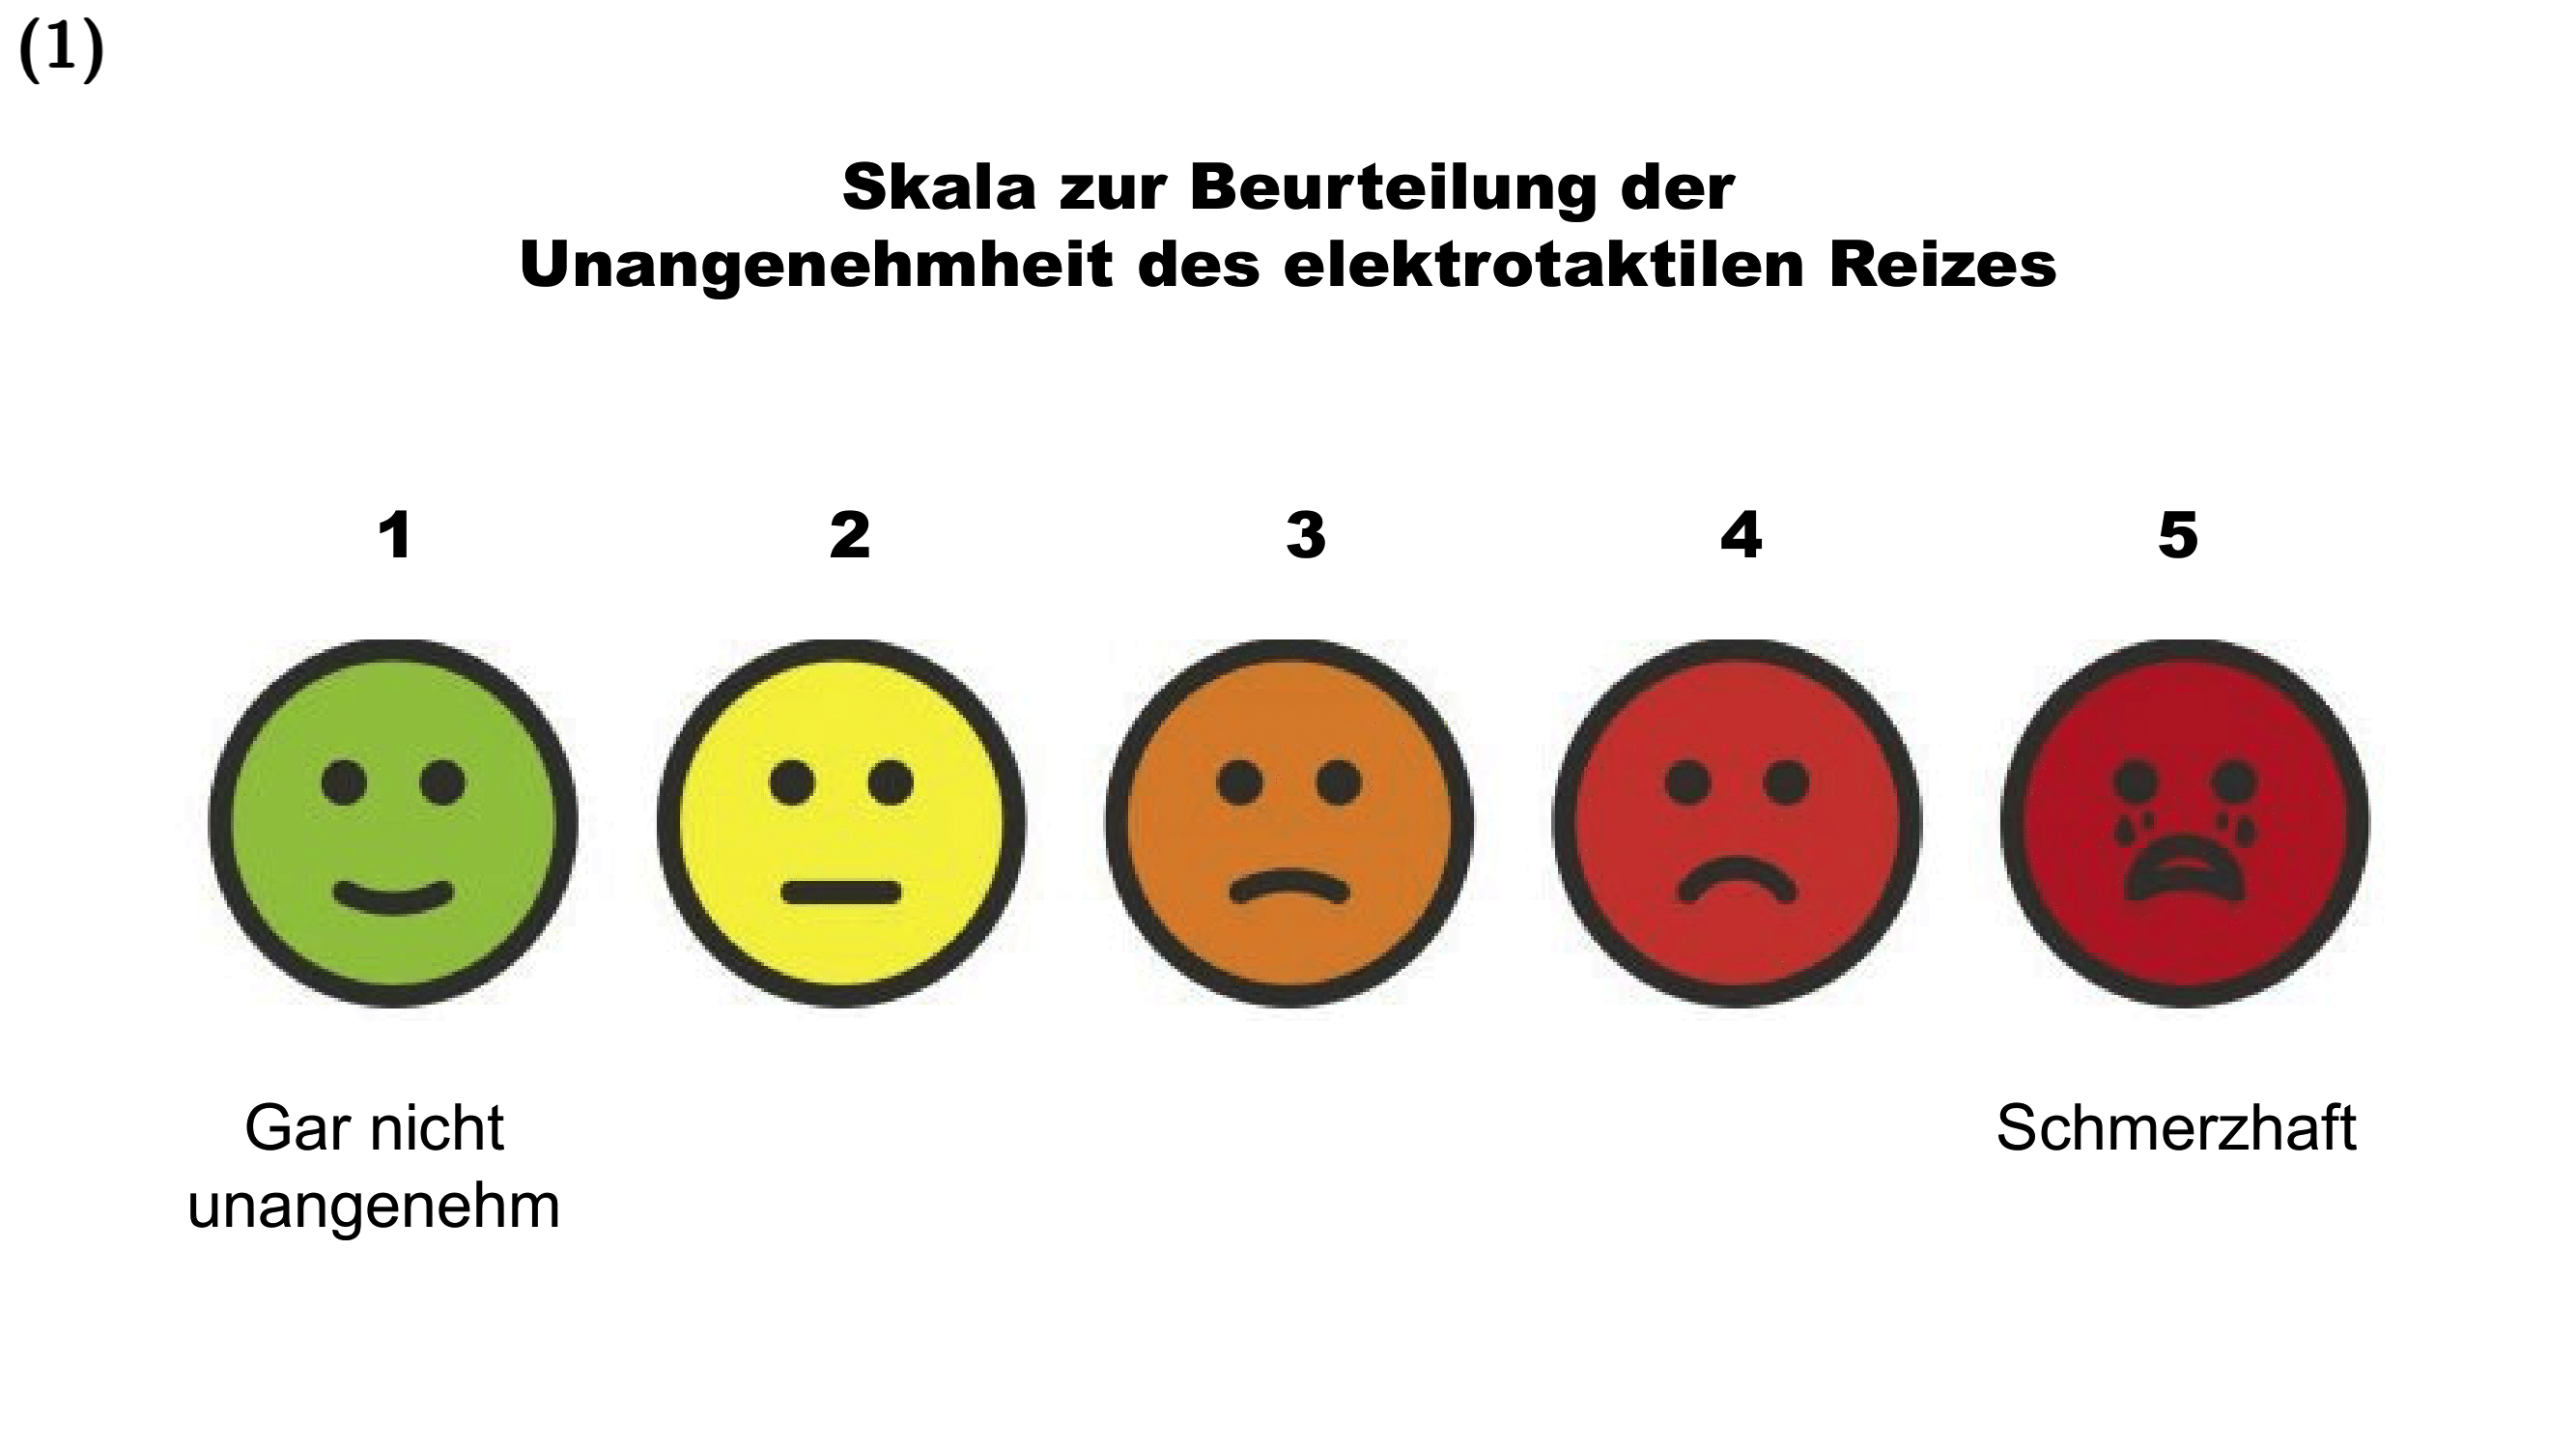
\includegraphics[width=\textwidth]{us_skala1.png}
	\end{minipage}

	\vspace*{1cm}
	\noindent\begin{minipage}[t]{14cm}
		\vspace*{0.5cm}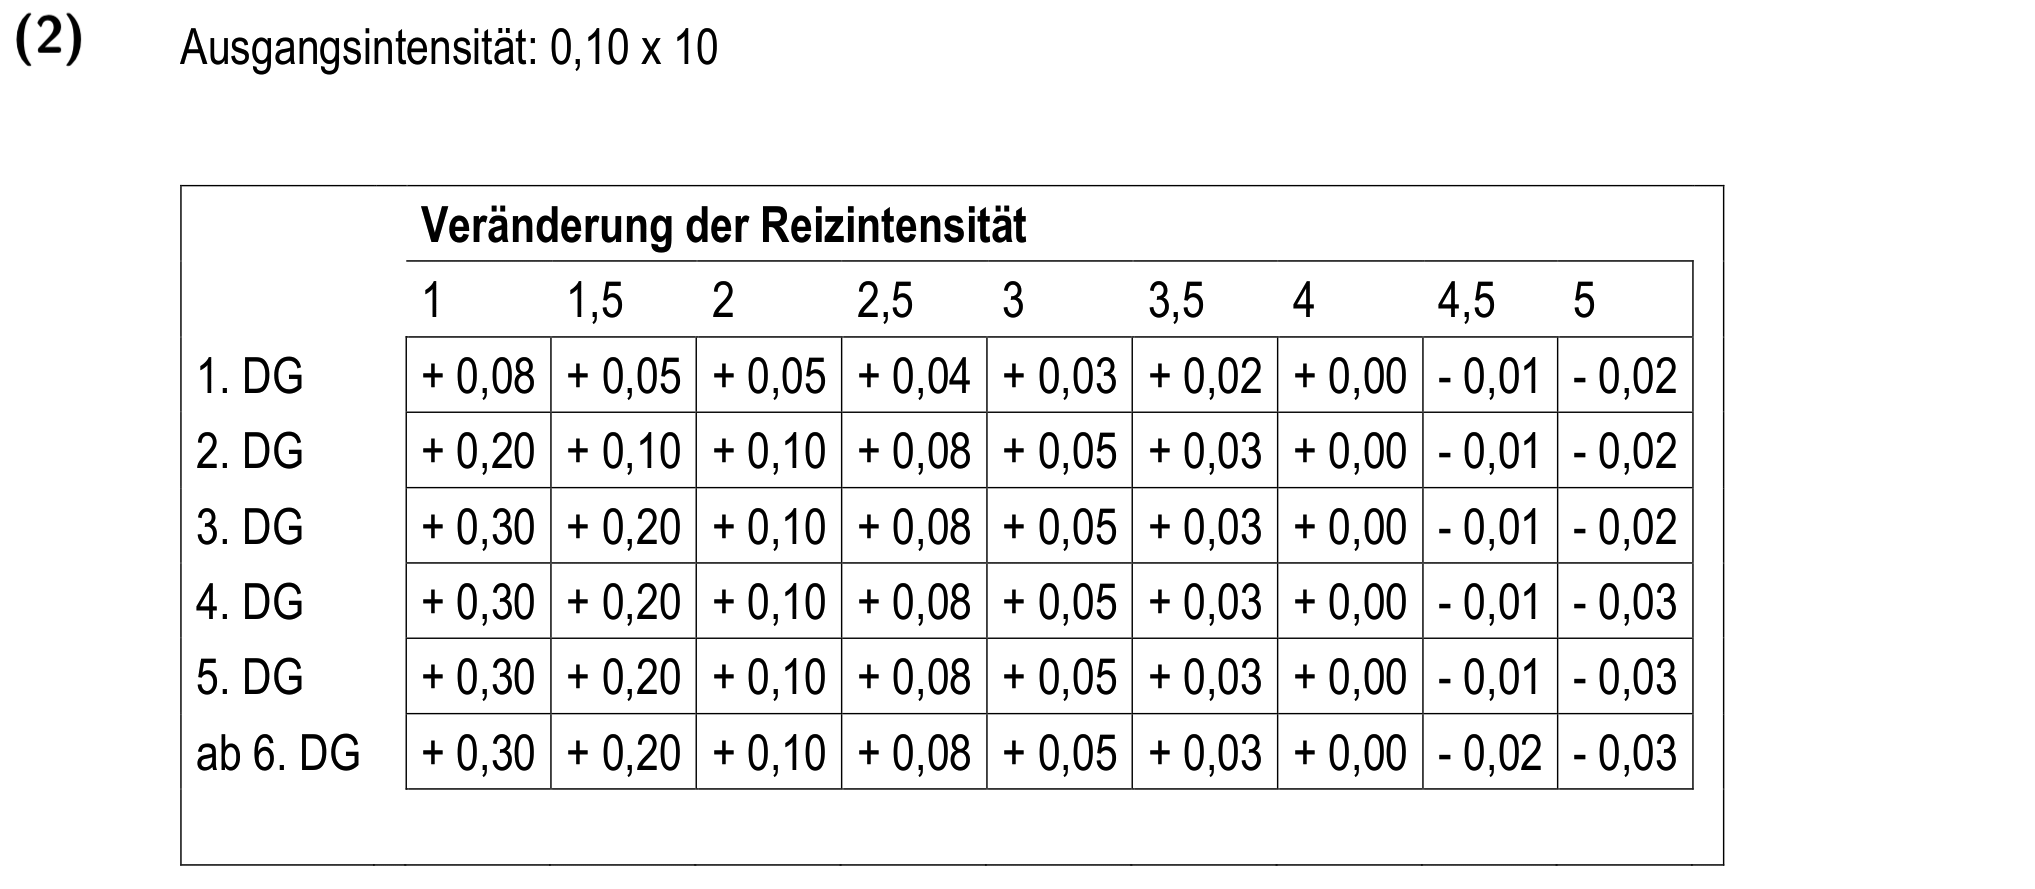
\includegraphics[width=\textwidth]{swu_tabelle1.png} 
	\end{minipage}
	\newpage
	

\section*{Anhang B} \label{appB}
	
	\noindent\textit{SAM-Skalen zur Einschätzung von Valenz und Erregung \parencite{BRADLEY1994}, deutsch adaptierte Fassung}
		
		\begin{minipage}[t]{0.95\textwidth}
			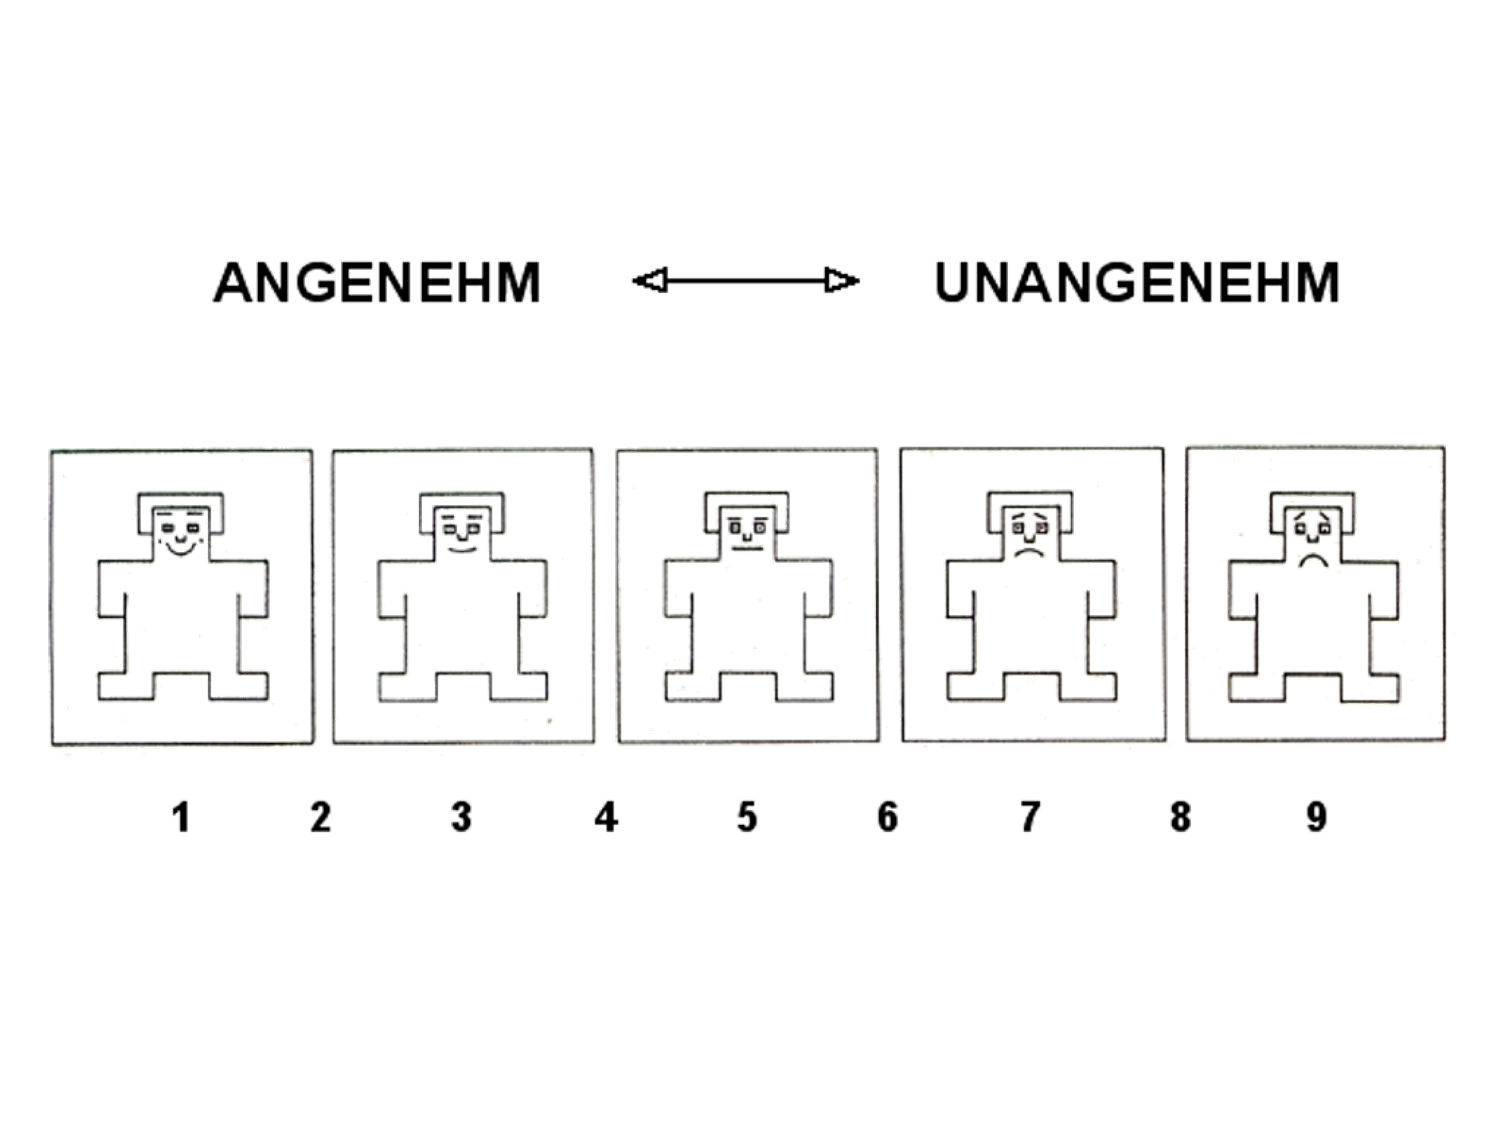
\includegraphics[width=0.9\textwidth]{SAM1} \vspace*{-1cm}
			
			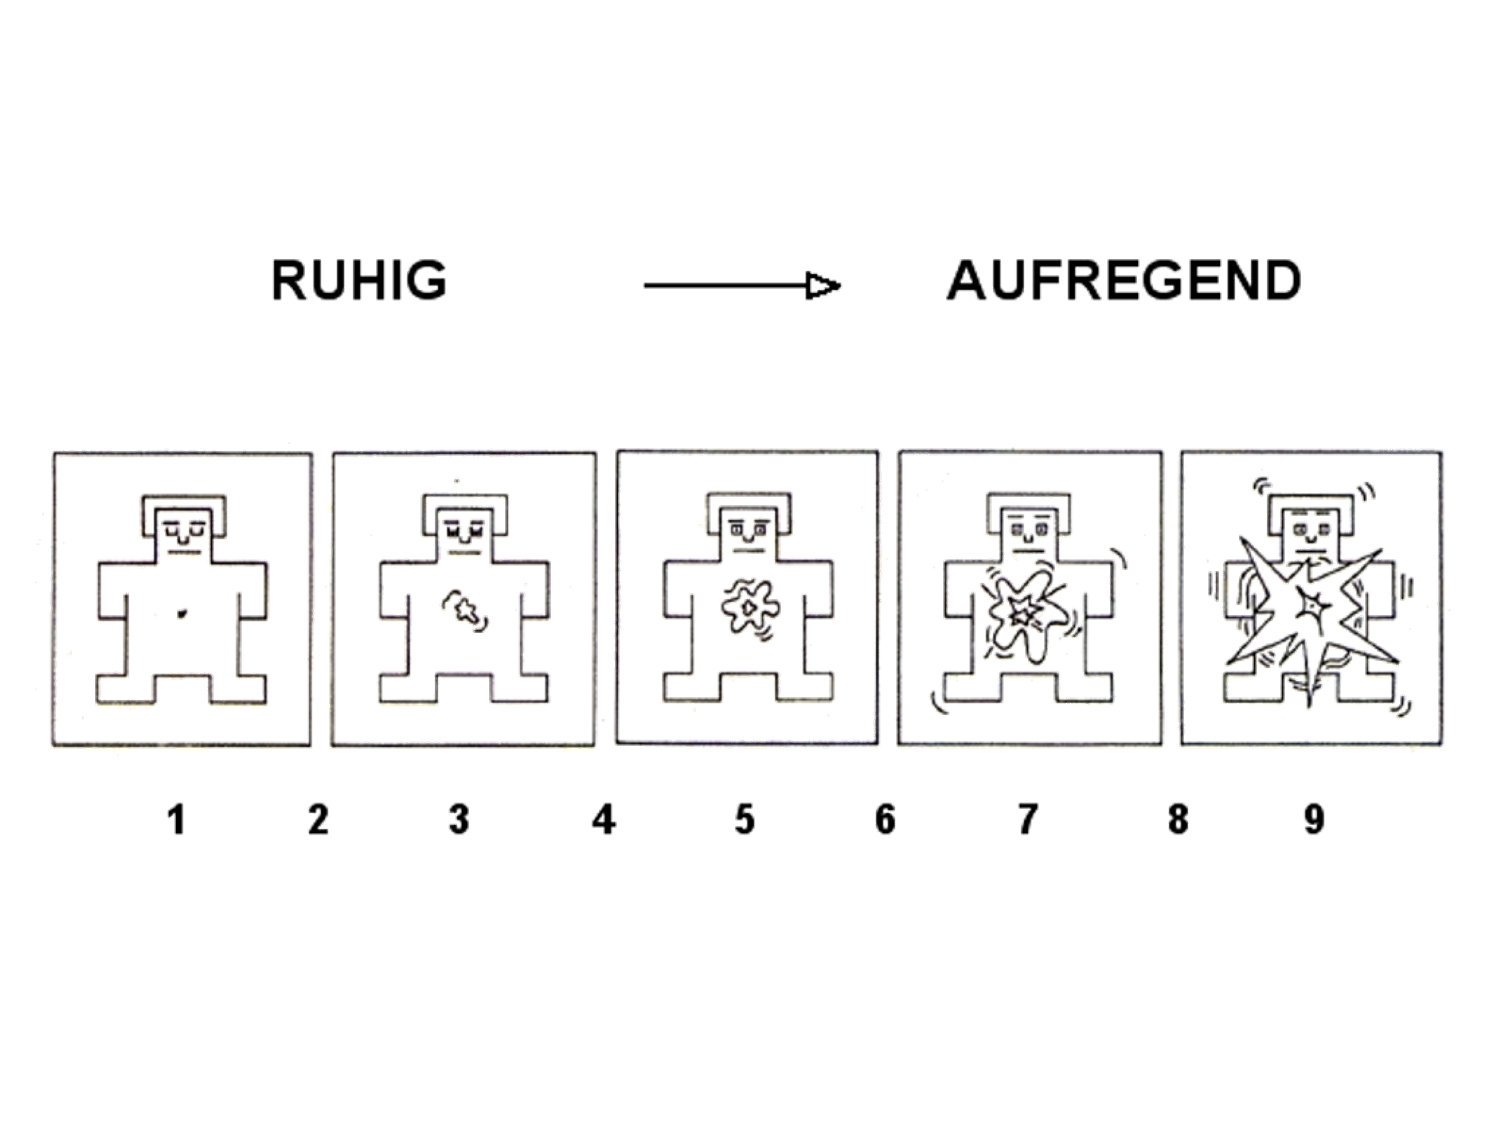
\includegraphics[width=0.9\textwidth]{SAM2}
		\end{minipage}
	\newpage


\section*{Anhang C} \label{appC}
	
	\noindent\textit{Streudiagramm zwischen Hautleitwert- und Schreckreaktionen. Die Gerade entspricht der Vorhersage eines einfachen linearen Modells mit \SI{95}{\percent}-Konfidenzgrenze}
		
		\vspace*{2cm}\hspace*{-0.5cm}
		\begin{minipage}[t]{0.95\textwidth}
			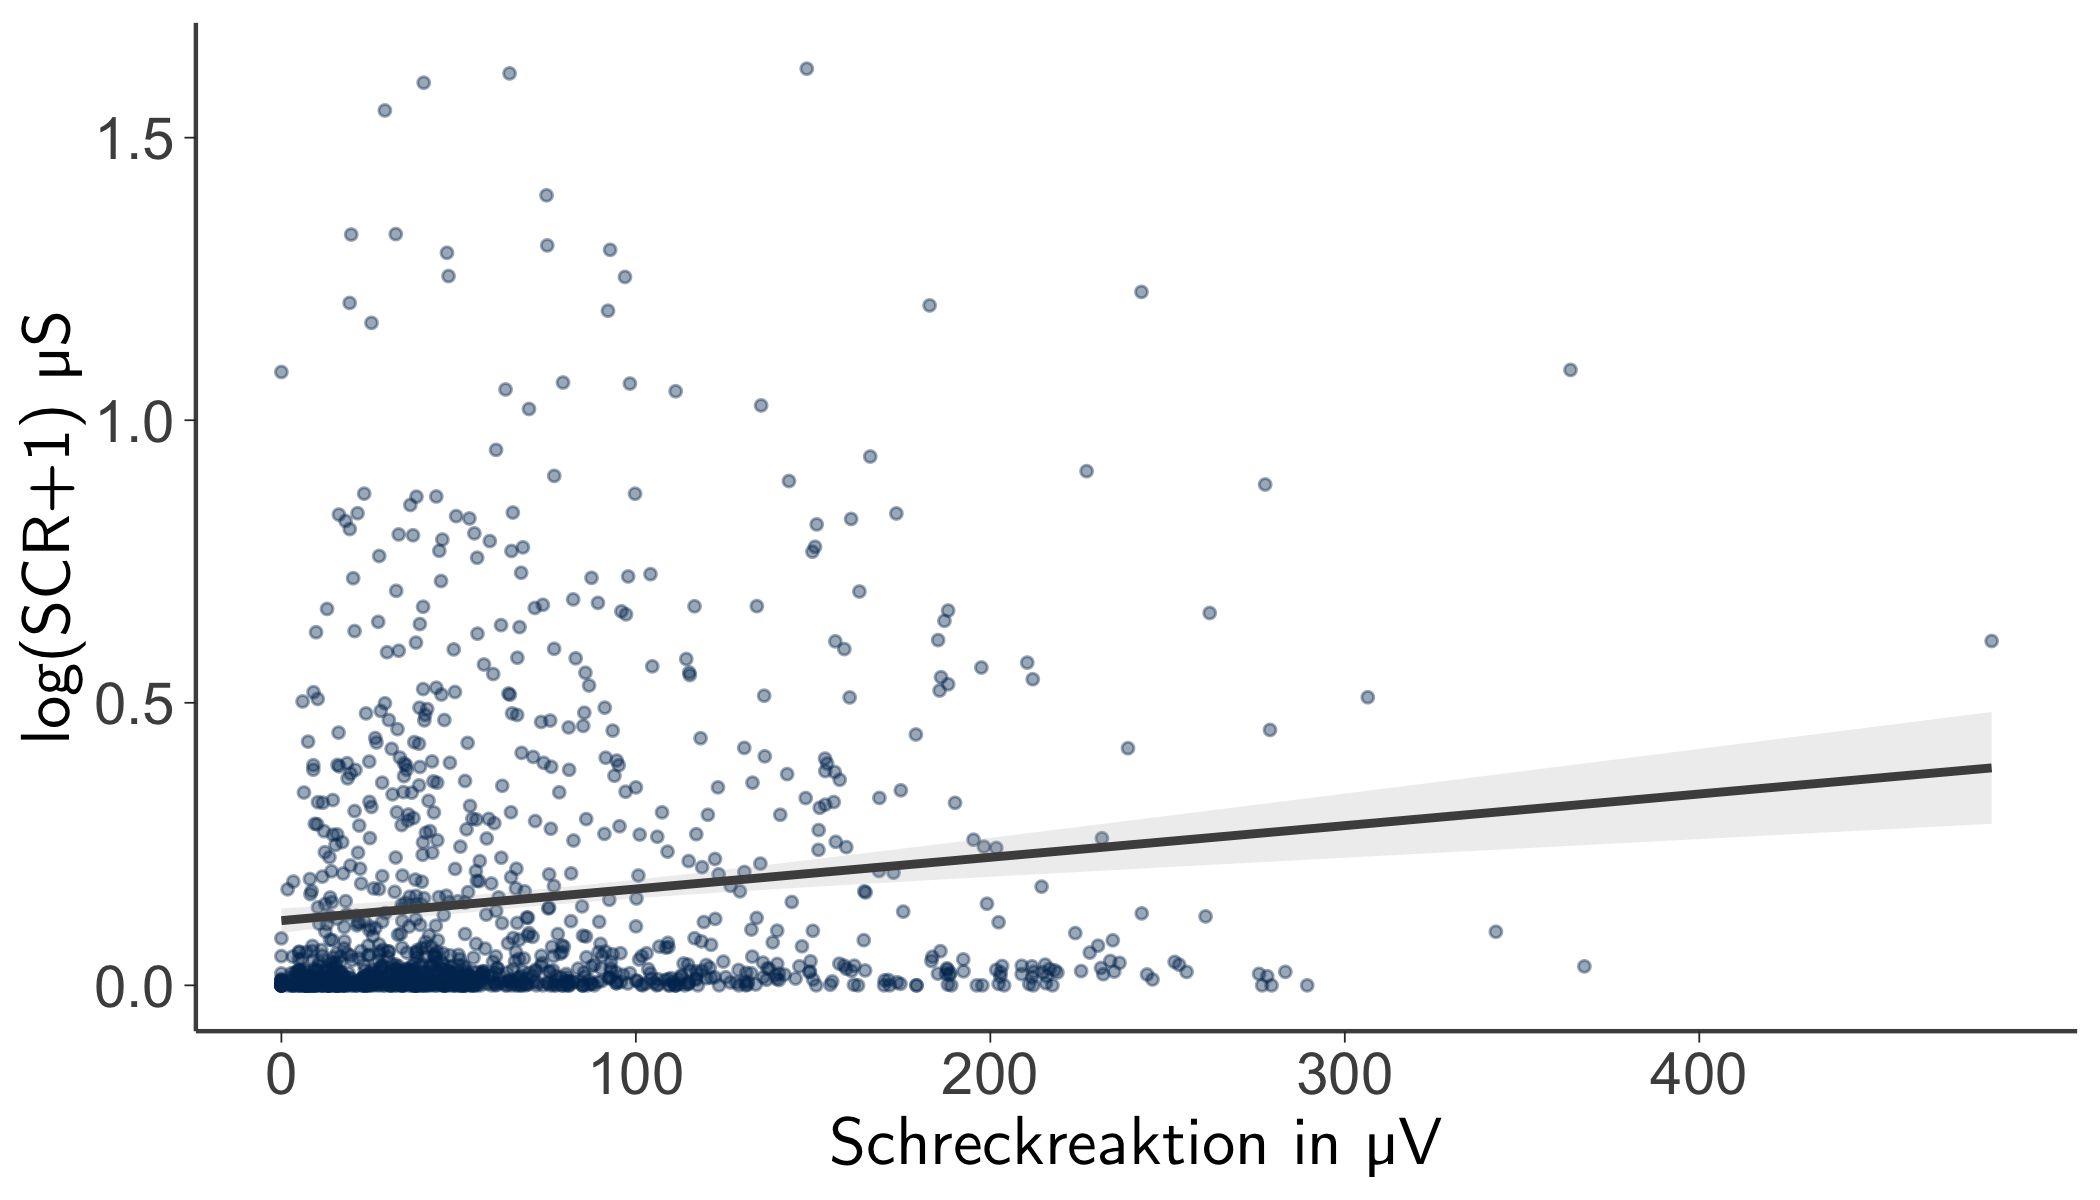
\includegraphics[width=0.9\textwidth]{multivariat1.png}
		\end{minipage}

	\newpage

\section*{Anhang D} \label{appD}

	\noindent \textit{Teststatistiken der Shapiro-Wilk-Tests für beide abhängigen Variablen}

	%\begin{table}[h]
	\vspace*{0.3cm}
		\begin{threeparttable}
			\begin{tabularx}{0.7\textwidth}{XCC}   \toprule
			 	Trial      	& SCR		 	& STR		\\ \hline \rowcolor[HTML]{EFEFEF}
			 	insgesamt  	& $0.64^{***}$		& $0.84^{***}$	\\
			 	 1 		& $0.81^{***}$  	& $0.81^{***}$	\\\rowcolor[HTML]{EFEFEF}
			 	 2 		& $0.68^{***}$  	& $0.91^{***}$	\\
			 	 3 		& $0.76^{***}$  	& $0.89^{***}$	\\\rowcolor[HTML]{EFEFEF}
			 	 4 		& $0.60^{***}$  	& $0.89^{***}$	\\
			 	 5 		& $0.61^{***}$  	& $0.87^{***}$	\\\rowcolor[HTML]{EFEFEF}
			 	 6 		& $0.67^{***}$  	& $0.77^{***}$	\\
			 	 7 		& $0.64^{***}$  	& $0.85^{***}$	\\\rowcolor[HTML]{EFEFEF}
			 	 8 		& $0.49^{***}$  	& $0.82^{***}$	\\
			 	 9  	& $0.78^{***}$  	& $0.82^{***}$	\\\rowcolor[HTML]{EFEFEF}
			 	 10 	& $0.66^{***}$  	& $0.79^{***}$  \\
			 	 11 	& $0.64^{***}$  	& $0.79^{***}$	\\\rowcolor[HTML]{EFEFEF}
			 	 12 	& $0.59^{***}$  	& $0.83^{***}$	\\
			 	 13 	& $0.59^{***}$  	& $0.86^{***}$	\\\rowcolor[HTML]{EFEFEF}
			 	 14 	& $0.62^{***}$  	& $0.80^{***}$	\\
			 	 15 	& $0.59^{***}$  	& $0.75^{***}$	\\\rowcolor[HTML]{EFEFEF}
			 	 16 	& $0.53^{***}$  	& $0.82^{***}$	\\\bottomrule
			\end{tabularx}
			\begin{tablenotes}[normal, flushleft, para]
				\footnotesize{\item \textit{Anmerkungen.} SCR: Hautleitwertreaktion, STR: Schreckreaktion; \\ ${}^{*}\, p<.05$, ${}^{**}\, p<.01$, ${}^{***}\, p<.001$.}
			\end{tablenotes}
		\end{threeparttable}
	%\end{table}		
	\newpage



\section*{Anhang E} \label{appE}

	\noindent\textit{Streudiagramme (und Korrelationen) zwischen den geschätzten zufälligen Effekten beider abhängiger Variablen}
	
	\vspace*{1cm}\hspace*{-0.5cm}
	\begin{minipage}{\textwidth}
			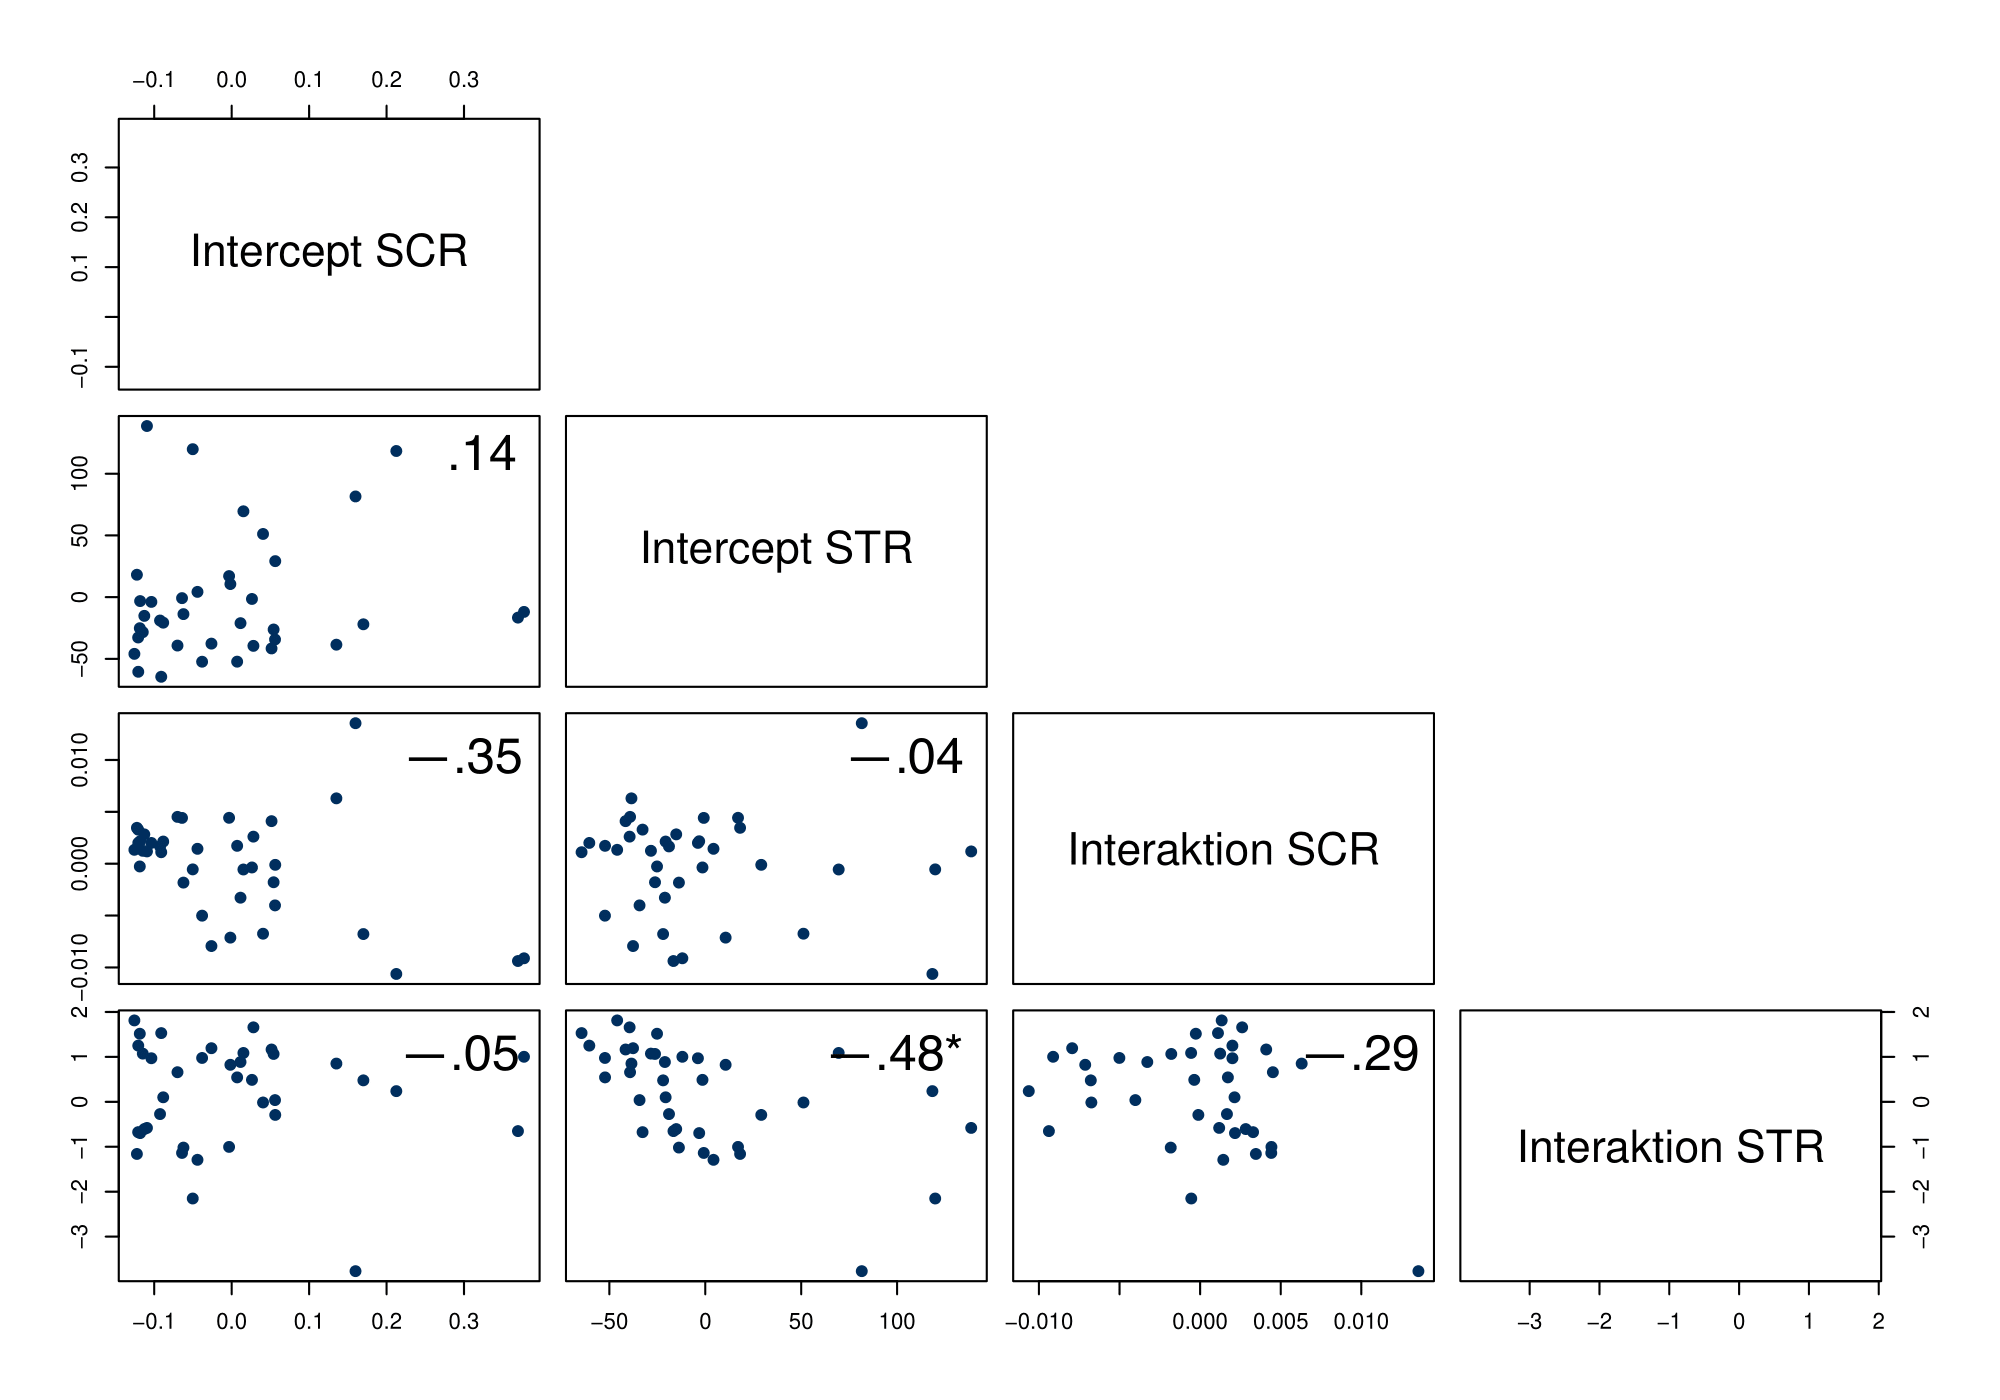
\includegraphics[width=\textwidth]{rescatter2.png}
	\end{minipage}


\section*{Anhang F} \label{appF}

\noindent\textit{Streudiagramme zwischen Residuen der höchsten Gruppierungsebene und angepassten Werten für beide AV (\textbf{a}, \textbf{b}) sowie  Q-Q-Diagramme (\textbf{c}, \textbf{d}) und Histogramme (\textbf{e}, \textbf{f}) dieser Residuen für beide AV}

\vspace*{0.5cm}\hspace*{-0.5cm}
\begin{minipage}[t]{\textwidth}
			\begin{tikzpicture}[remember picture] \centering		
			\node[inner sep=0pt] (a1) at (0,0)
			{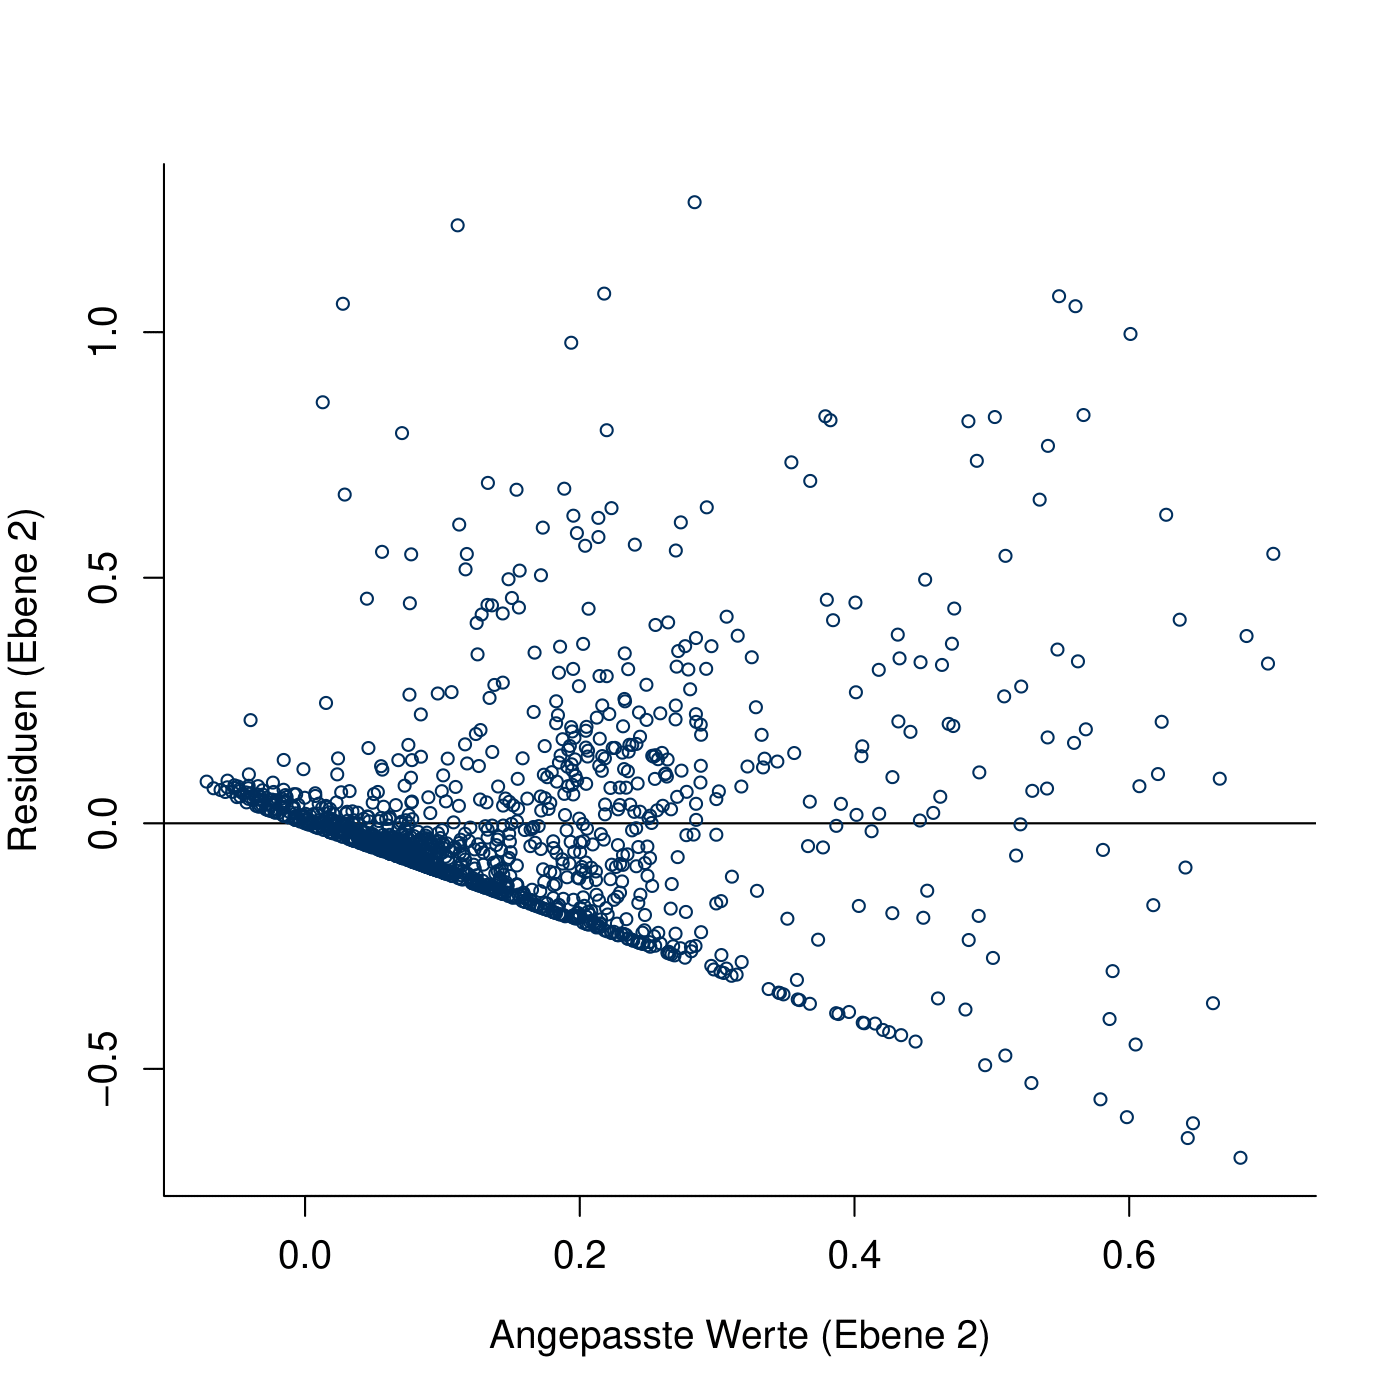
\includegraphics[scale=0.135]{as_scr_1.png}};
			\node[inner sep=0pt, right = 1cm of a1] (a2)
			{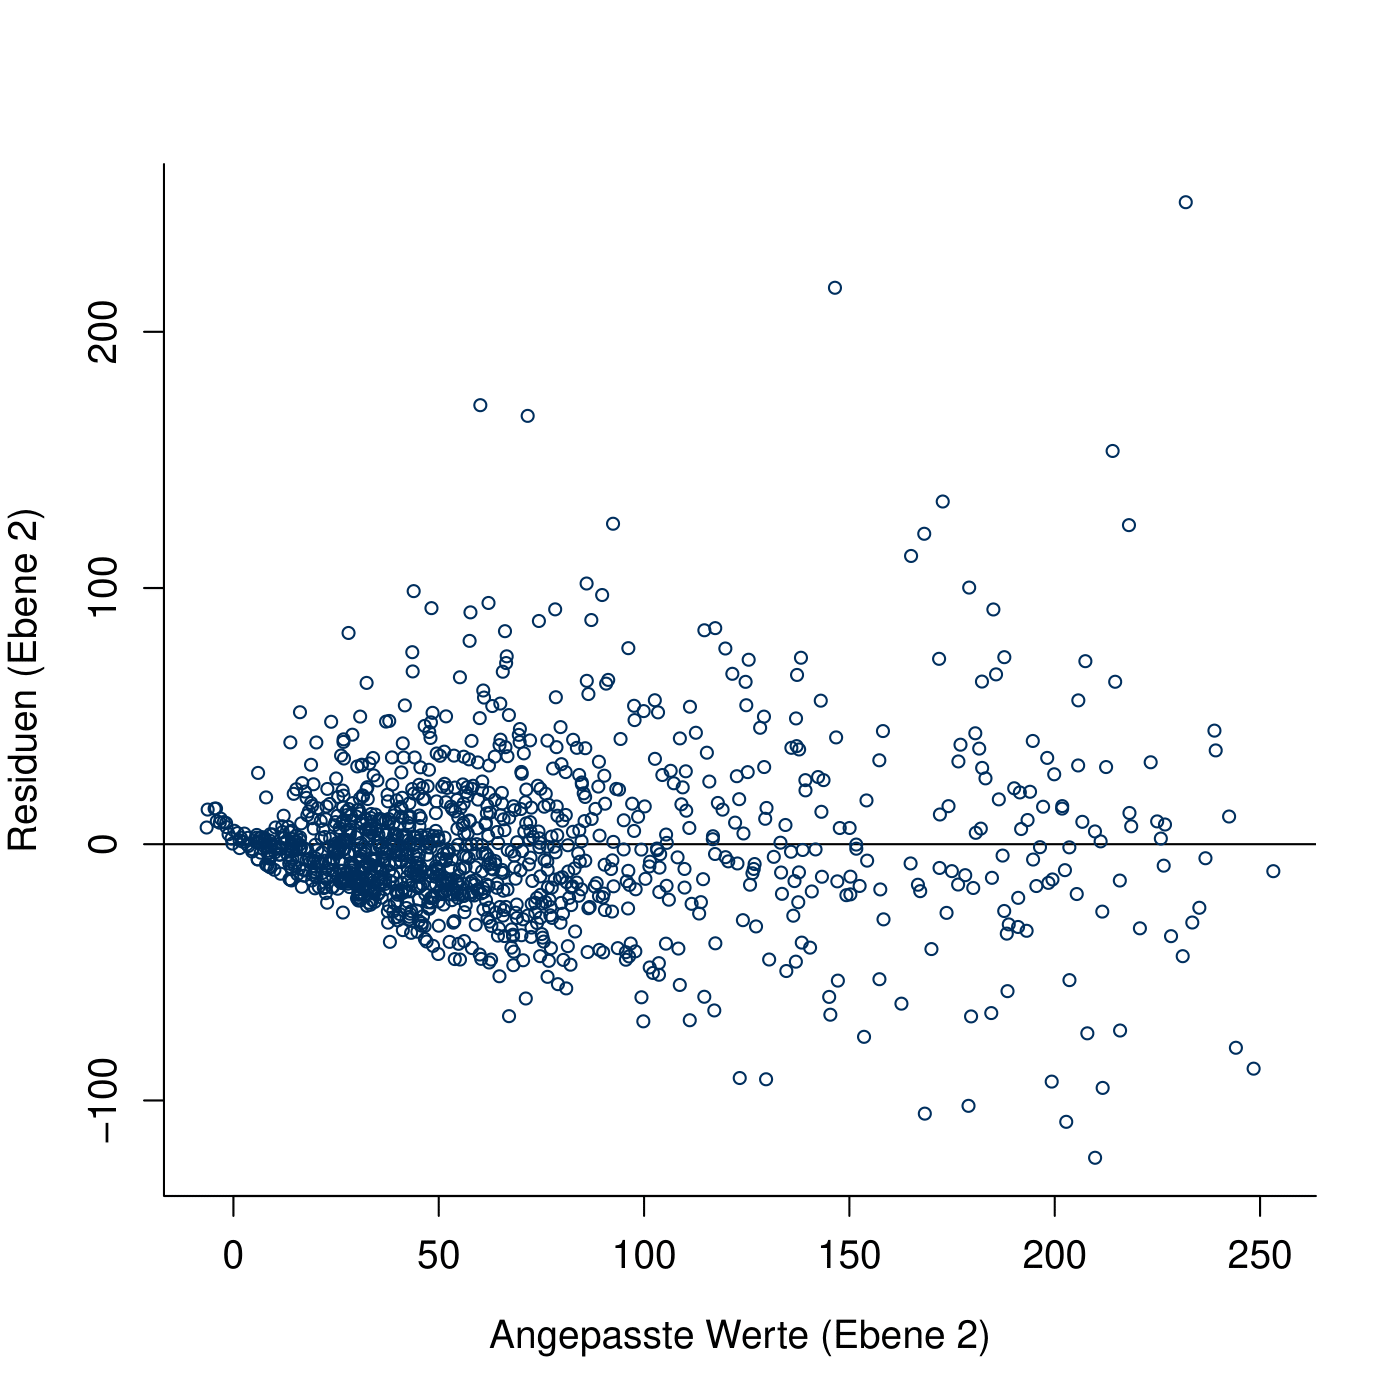
\includegraphics[scale=0.135]{as_str_1.png}};			
			\node[inner sep=0pt, below = 0.3cm of a1] (a3)
			{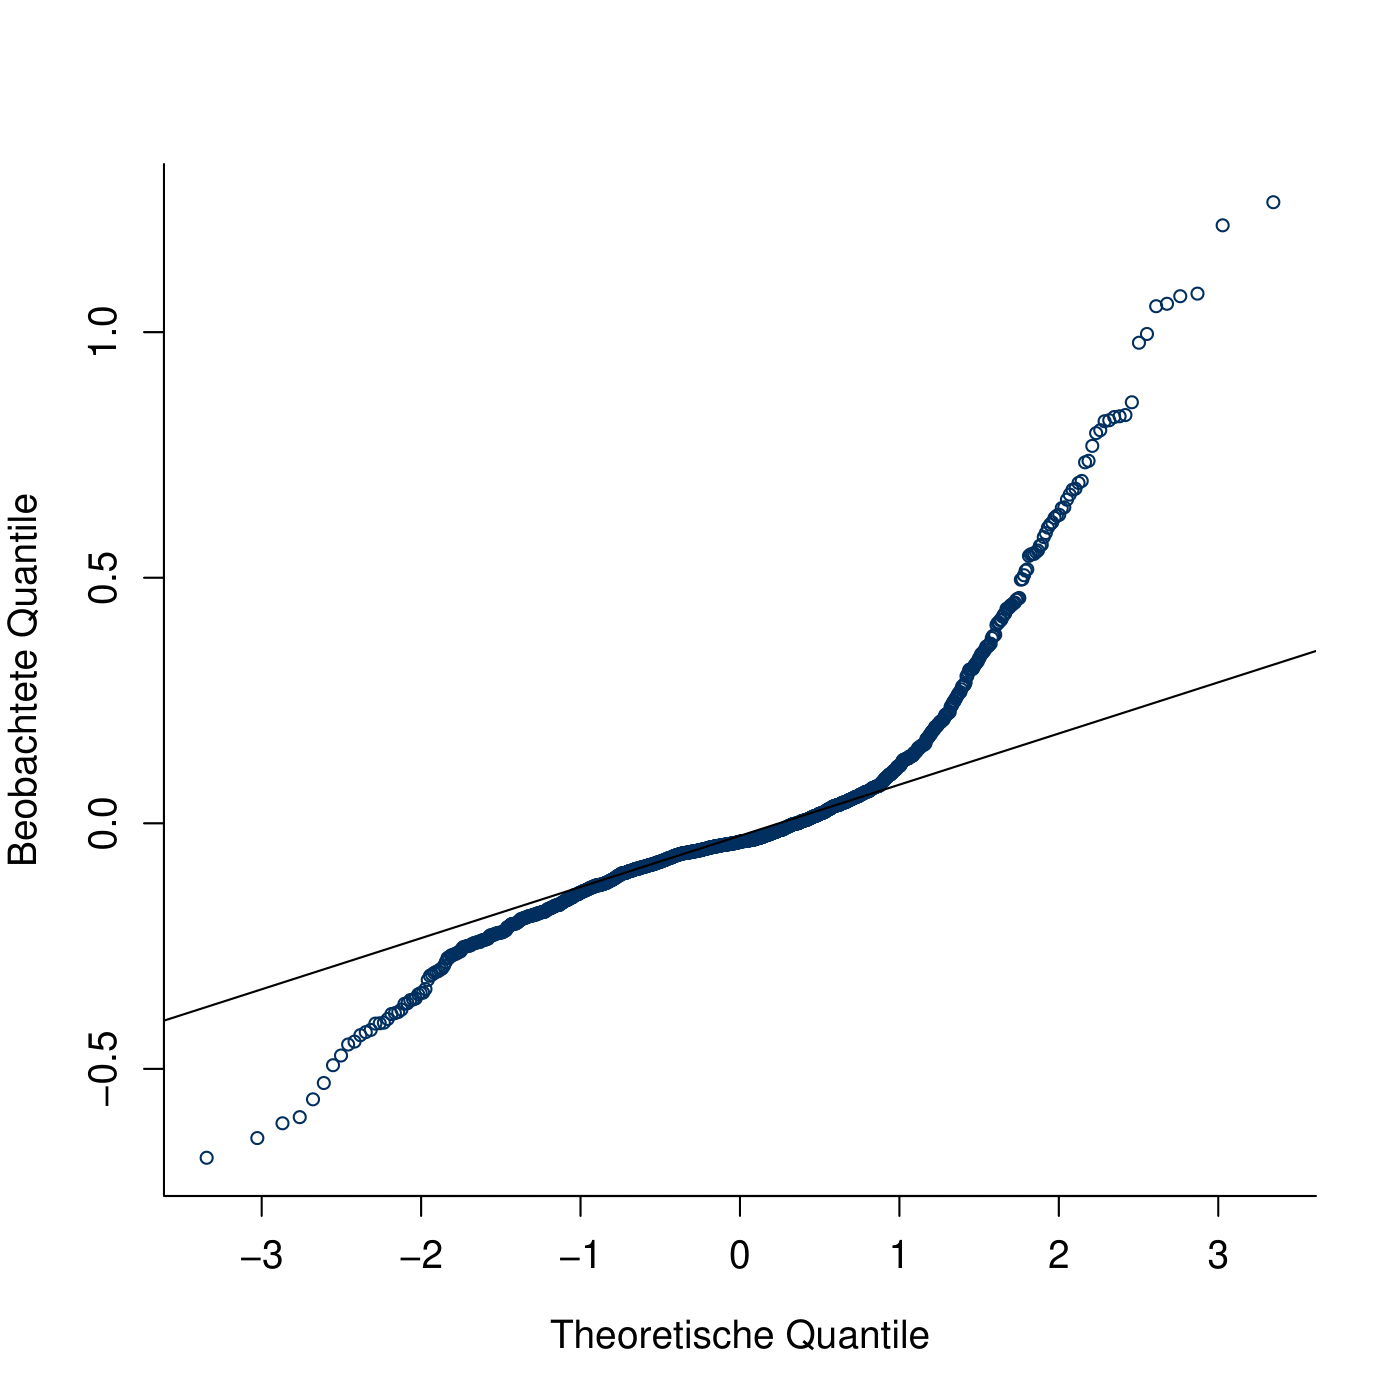
\includegraphics[scale=0.135]{qq_scr_1.png}};
			\node[inner sep=0pt, below = 0.3cm of a2] (a4)
			{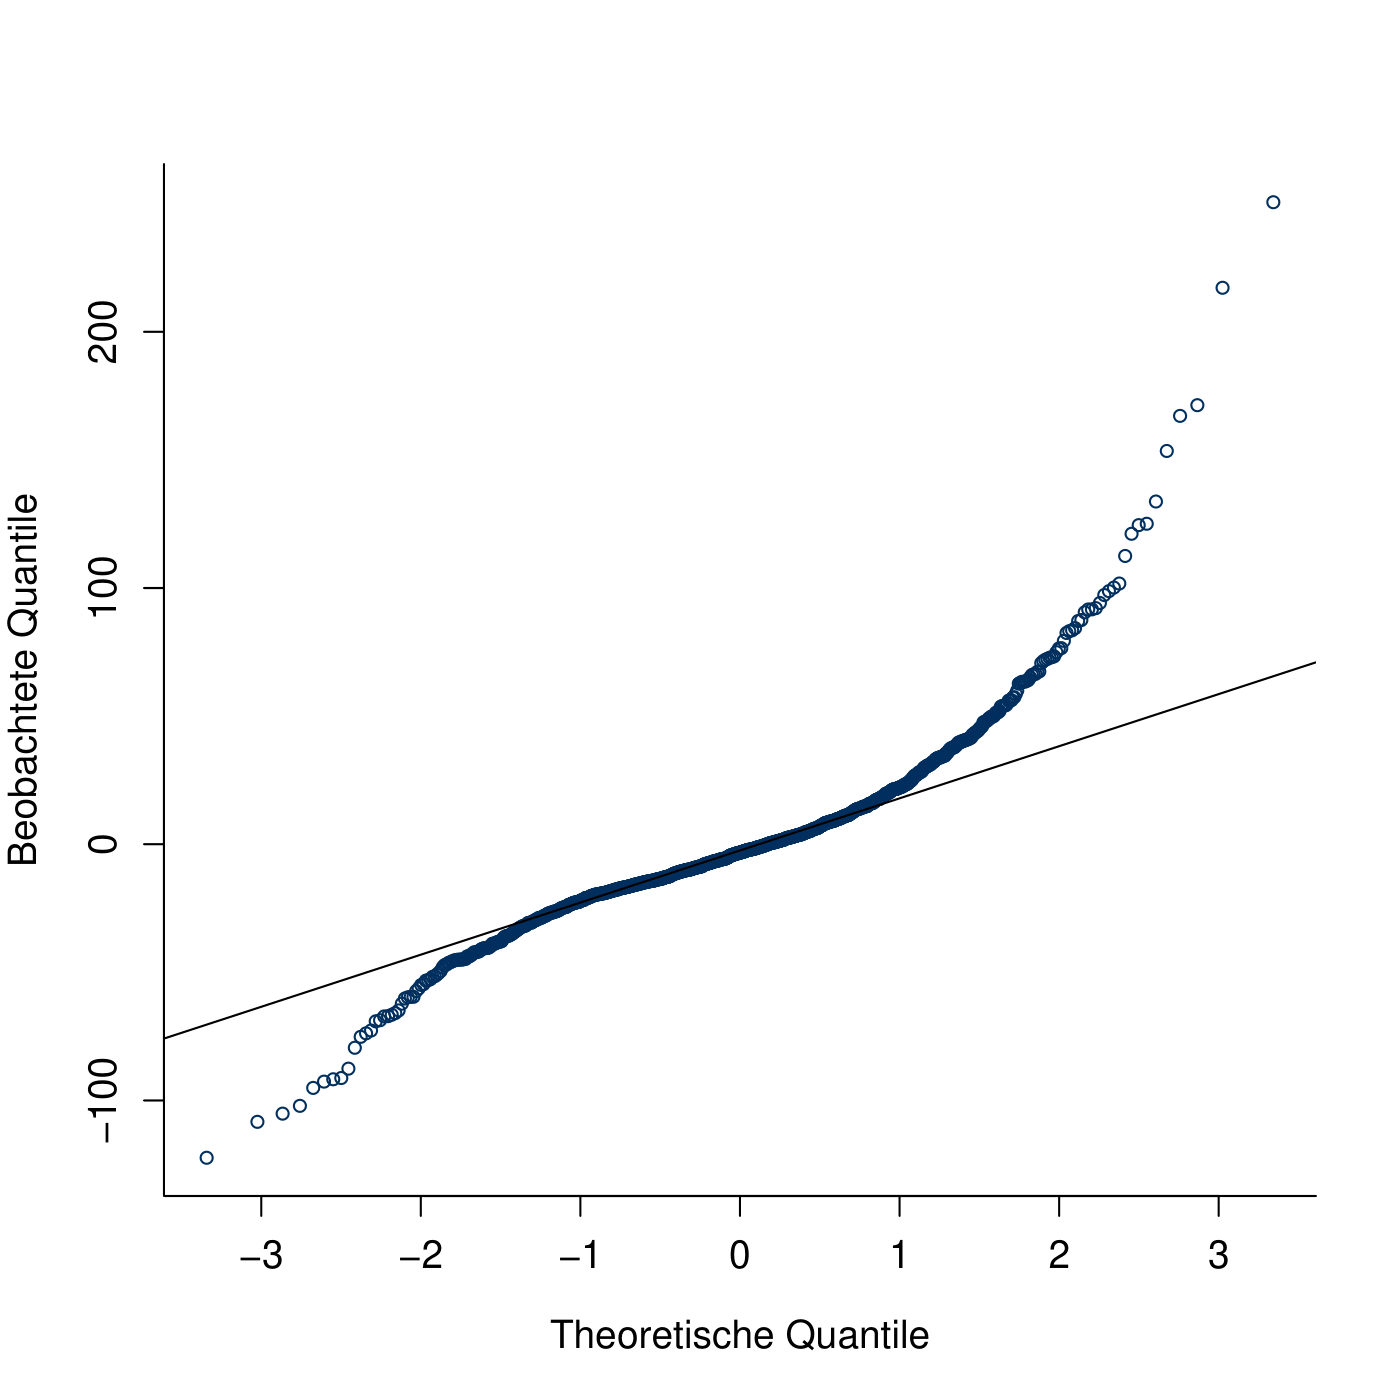
\includegraphics[scale=0.135]{qq_str_1.png}};
			\node[inner sep=0pt, below = 0.3cm of a3] (a5)
			{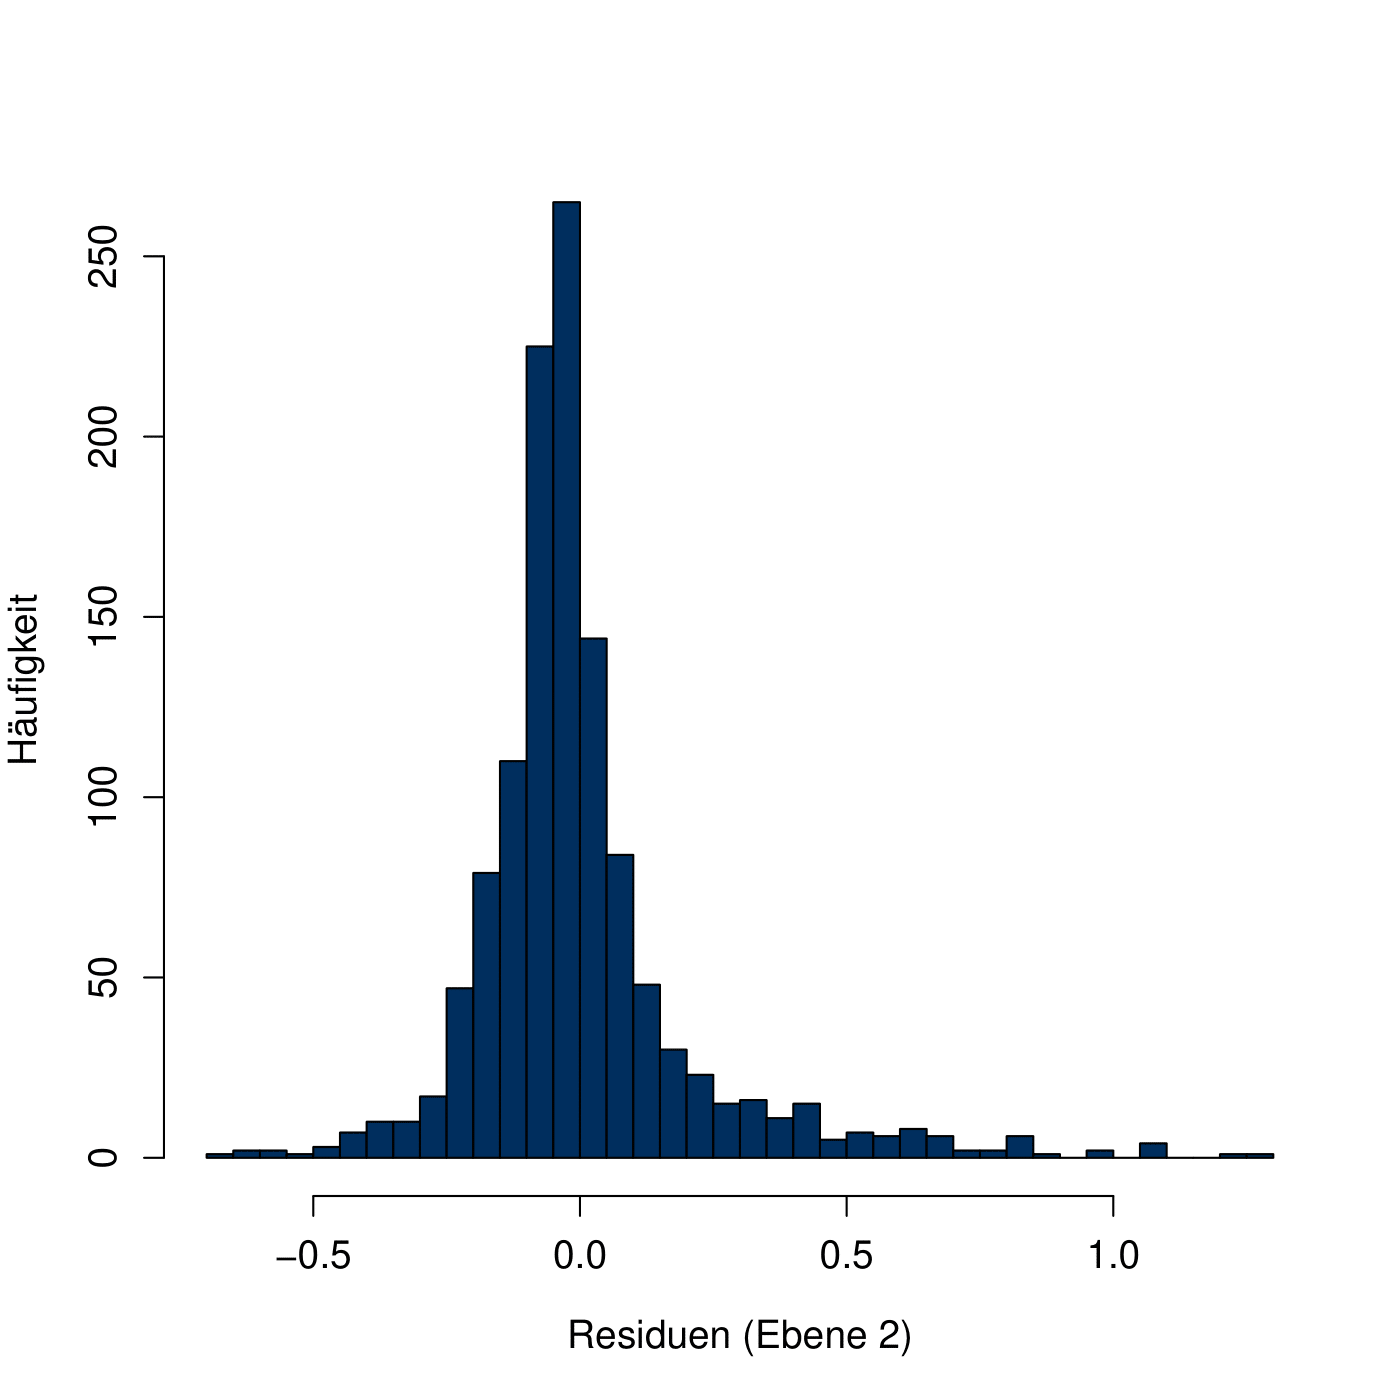
\includegraphics[scale=0.135]{his_scr_1.png}};
			\node[inner sep=0pt, below = 0.3cm of a4] (a6)
			{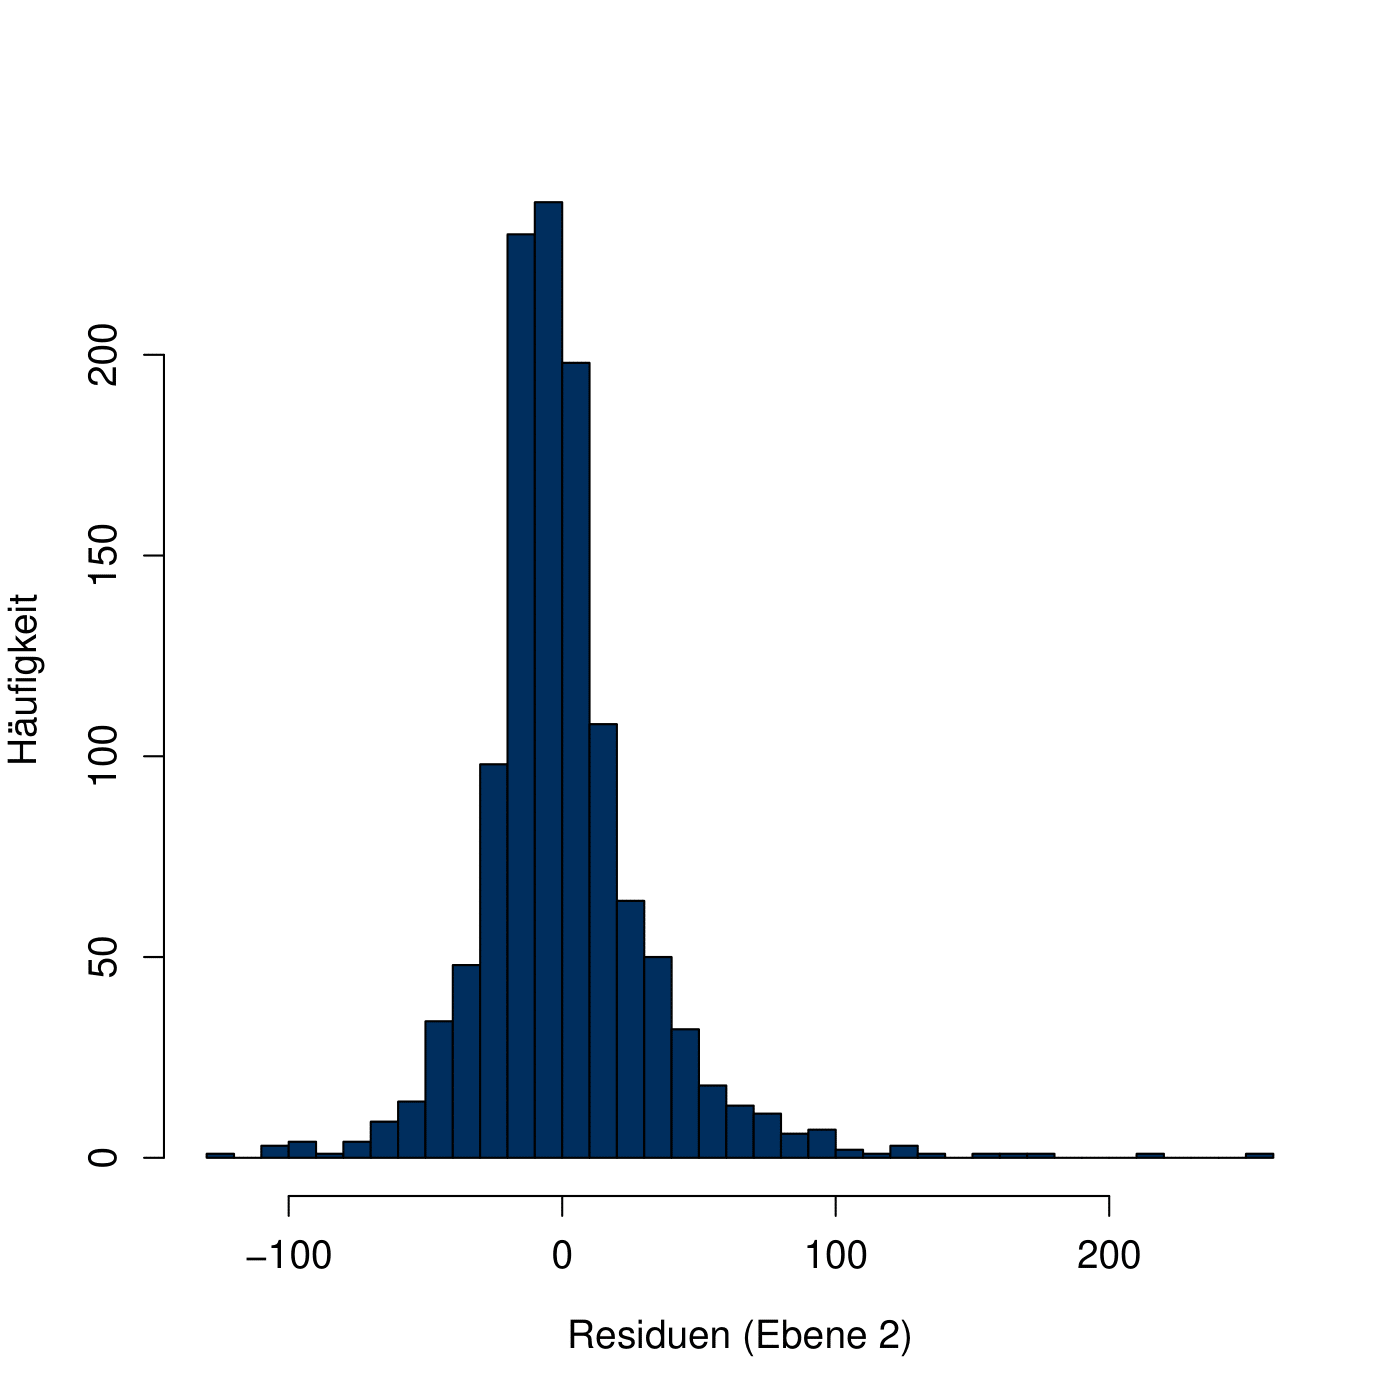
\includegraphics[scale=0.135]{his_str_1.png}};
			\node[above = 0.3cm of a1] (SCR) {\large{\textsf{\textbf{SCR}}}};
			\node[above = 0.3cm of a2] (STR) {\large{\textsf{\textbf{STR}}}};
			\node[above left = 0cm and -0.5cm of a1] (a) {\large{\textsf{\textbf{a}}}};
			\node[above left = 0cm and -0.5cm of a2] (b) {\large{\textsf{\textbf{b}}}};
			\node[above left = 0cm and -0.5cm of a3] (c) {\large{\textsf{\textbf{c}}}};
			\node[above left = 0cm and -0.5cm of a4] (d) {\large{\textsf{\textbf{d}}}};
			\node[above left = 0cm and -0.5cm of a5] (e) {\large{\textsf{\textbf{e}}}};
			\node[above left = 0cm and -0.5cm of a6] (f) {\large{\textsf{\textbf{f}}}};
		\end{tikzpicture}
\end{minipage}

		
%		\begin{enumerate}
%			\item ...
%			\item R-Code auf Stick
%			\item Matlab Codes auf Stick
%		\end{enumerate}
	
	%\noindent\textit{Hygieneverordnung Departement 09.05.2020 (auf Stick?)}
					
			\addchap{Selbstständigkeitserklärung}
				\noindent 
Hiermit erkläre ich,
		\begin{center}
			Neele Katharina Elbersgerd, geboren am xx.xx.xxxx 
		\end{center} 
\noindent 
an Eides statt, dass ich die vorliegende Arbeit 
		\begin{center}
			\textit{Vergleich der Verläufe von Schreck- und Hautleitwertreaktionen \\in der Akquisitionsphase einer Furchtkonditionierung}
		\end{center}
\noindent 
selbstständig und ohne Benutzung von anderen als den angegebenen Hilfsmitteln und Quellen angefertigt habe. Alle Inhalte, die ich aus anderen veröffentlichten oder unveröffentlichten Quellen dem Wortlaut oder dem Sinne nach entnommen habe, sind kenntlich gemacht und im Literaturverzeichnis aufgeführt. Diese Arbeit wurde nicht im Rahmen eines anderen Prüfungsverfahrens eingereicht.
\newline
\vspace*{1cm}

\noindent Ort, Datum\\
\rule[0.5em]{30em}{0.5pt} % This prints a line for the signature

\vspace*{0.5cm}
\noindent Unterschrift\\
\rule[0.5em]{30em}{0.5pt} % This prints a line to write the date


%--------ENDE DES DOKUMENTS
\end{document}